
\chapter{Results}
\label{chap:results}

\section{Methodology}
For the purpose of reproducible evaluation, a JSON-configurable CLI tool was used to generate all results presented in this thesis and the exact parametrization is distributed along the source code on my repository \parencite{stamm2025}.

\paragraph{Performance Measurement}
Cuda Events are used to evaluate performance.
Tone mapping and screen blitting are not included into the measurements, so only the pure rendering time is reported.
If not otherwise stated, all measurements are taken on an NVIDIA RTX 3060 Ti GPU and averaged over at least 10 seconds.

\paragraph{Error Metric}
Reference images are generated using Path Tracing (PT) or Stochastic Progressive Photon Mapping (SPPM) \parencite{hachisuka2009a} in caustic scenes where PT does not converge.
To compare the quality of different techniques, the Mean Squared Error (MSE) in linear RGB space is reported for numerical error and the HDR variant of the \FLIP metric \parencite{andersson2021} for humanly perceived error.
Furthermore, bias and variance are measured separately by computing the first and second moment over 1000 independent 1spp renders.
Between the bias and variance samples the configuration and cache are kept constant, but for the inference pass different samples are drawn from a Quasi-Random Low Discrepancy Sequence.

\paragraph{Scenes}
Tests are performed on a set of scenes that are also included in the source code repository \parencite{stamm2025}:
\begin{itemize}
\item The \emph{Diffuse} scene is an adaptation of the Cornell Box and highlights diffuse indirect illumination.
\item The \emph{Thinker} scene incorporates glossy and transmissive materials with complex specular highlights.
It contains decimated and remeshed version of the Thinker statue by Auguste Rodin scanned by \textcite{scantheworld2014} and the Stanford Bunny scanned by \textcite{stanforduniversitycomputergraphicslaboratory1994}.
\item The \emph{Chess} scene is a complex textured scene composed of public domain assets from \textcite{polyhaven}.
\item The \emph{Ajar} scene is mostly lit by long indirect light paths, which are difficult to find with eye tracing.
\item The \emph{Caustics} scene contains complex sharp caustic patterns that are challenging for traditional path tracing.
\end{itemize}

\section{Inference}

\paragraph{Path Termination Strategies}

\begin{figure}[ht]
    \centering
    \tiny
    \begin{tabularx}{\textwidth}{r*{7}{>{\centering\arraybackslash}X}}
        & Reference (PT) & PT & 1st Vert & 1st Diff & SAH & BTH $1/2$ & BTH $1/10$ \\
        &2879spp (1m)
 & 1spp (20.96ms)
 & 1spp (11.46ms)
 & 1spp (11.35ms)
 & 1spp (10.83ms)
 & 1spp (10.77ms)
 & 1spp (\textbf{10.40ms})
\\
\rotatebox{90}{\textsc{Thinker}}\hspace{-1.5em}
&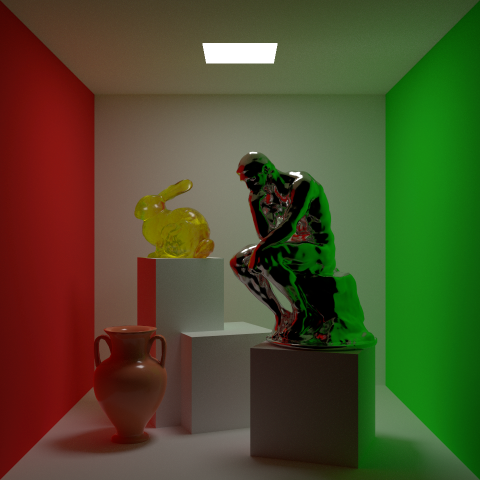
\includegraphics[width=\linewidth]{figures/py/tests/path_termination/ref_1min_thinker.png}
& 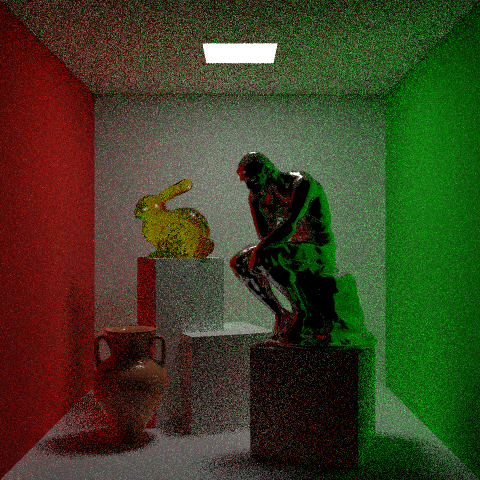
\includegraphics[width=\linewidth]{figures/py/tests/path_termination/ref_1spp_thinker.png}
& 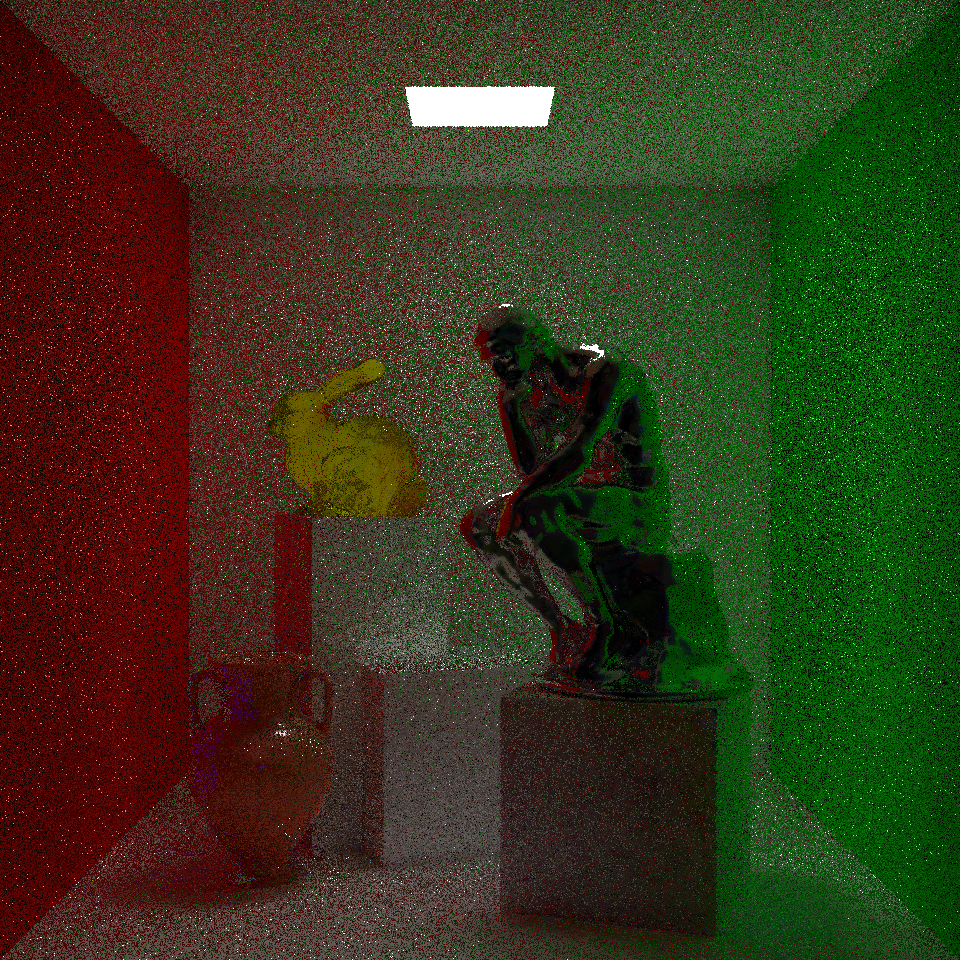
\includegraphics[width=\linewidth]{figures/py/tests/path_termination/sah_1spp_thinker.png}
& 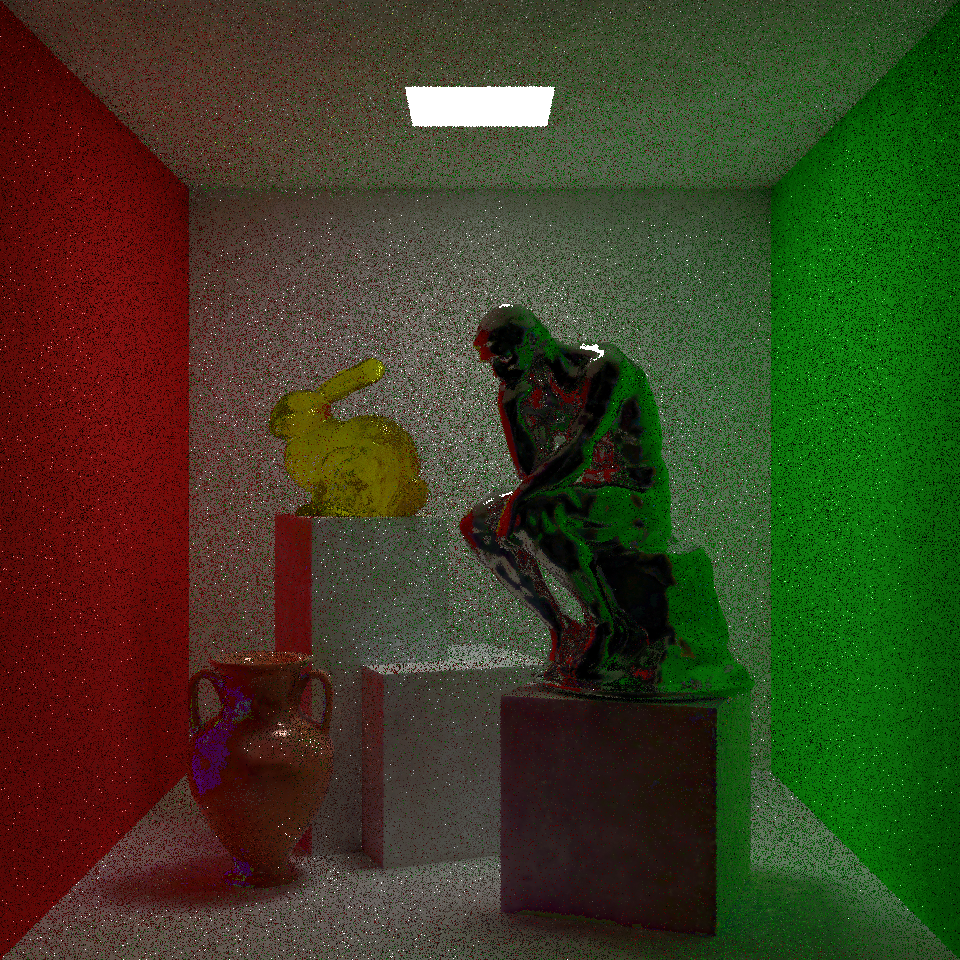
\includegraphics[width=\linewidth]{figures/py/tests/path_termination/bth_1spp_thinker.png}
& 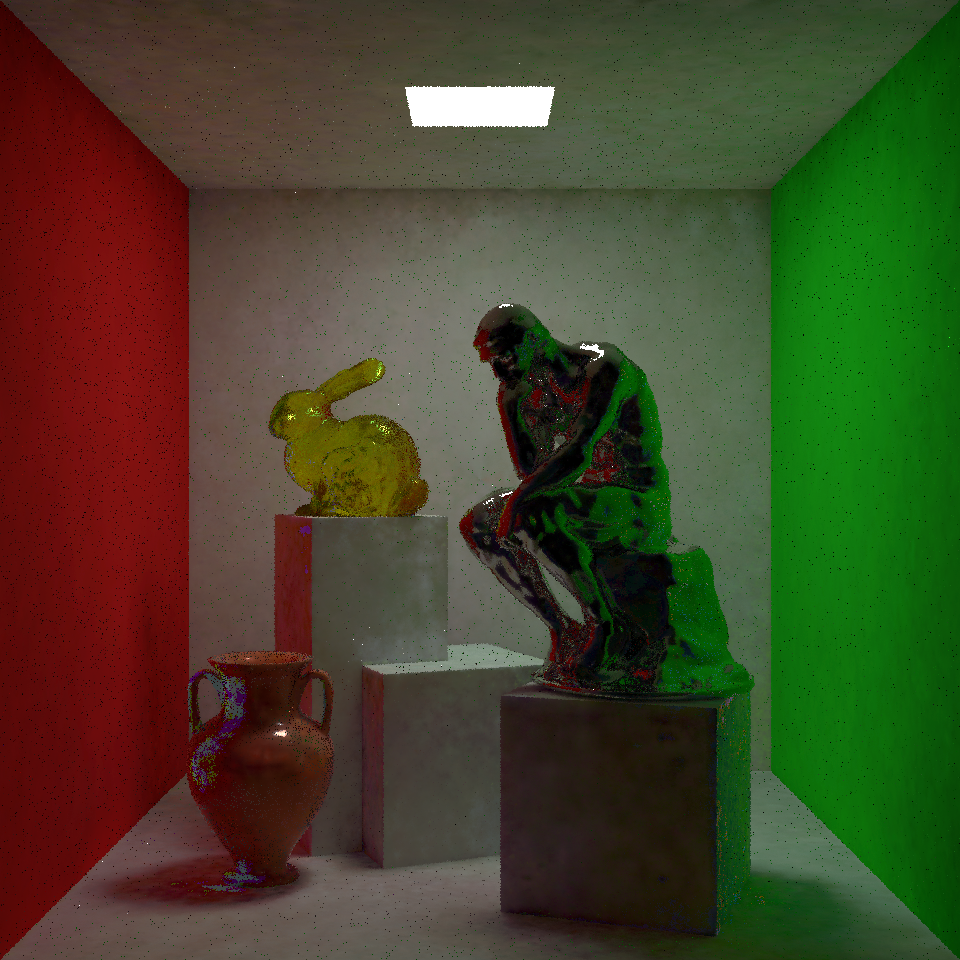
\includegraphics[width=\linewidth]{figures/py/tests/path_termination/bthk9_1spp_thinker.png}
& 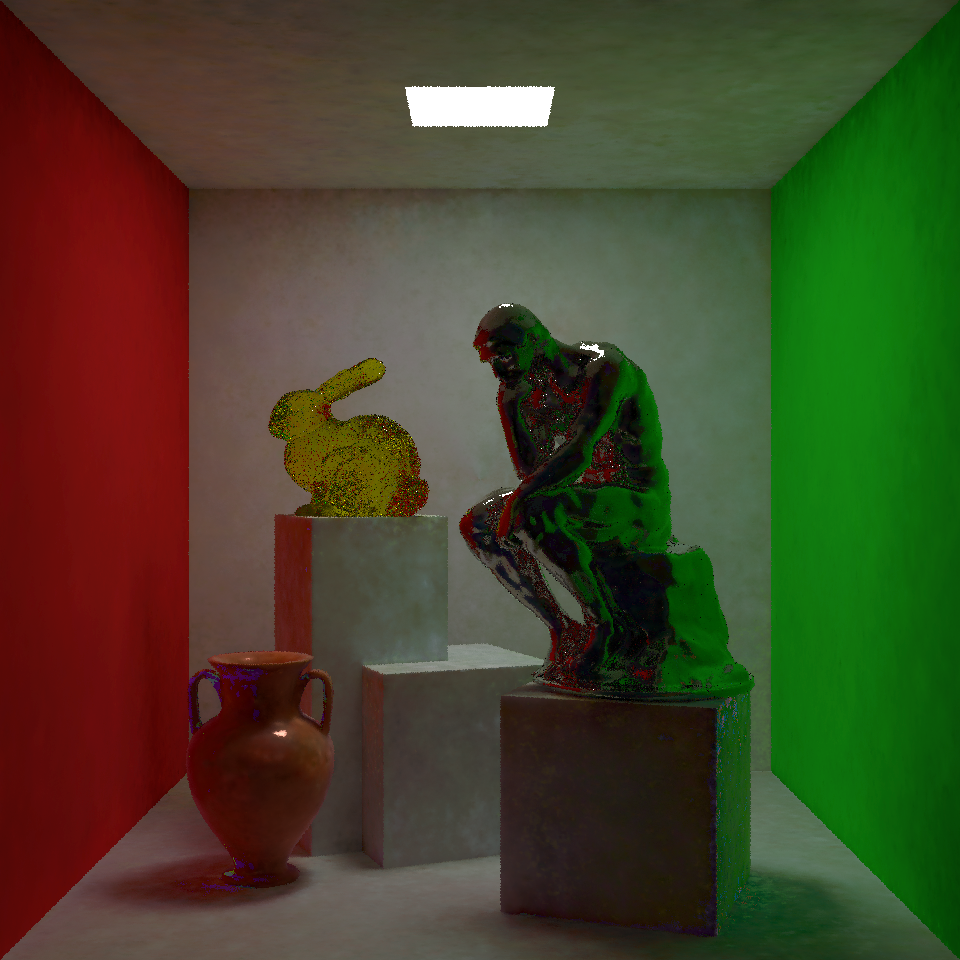
\includegraphics[width=\linewidth]{figures/py/tests/path_termination/1stdiff_1spp_thinker.png}
& 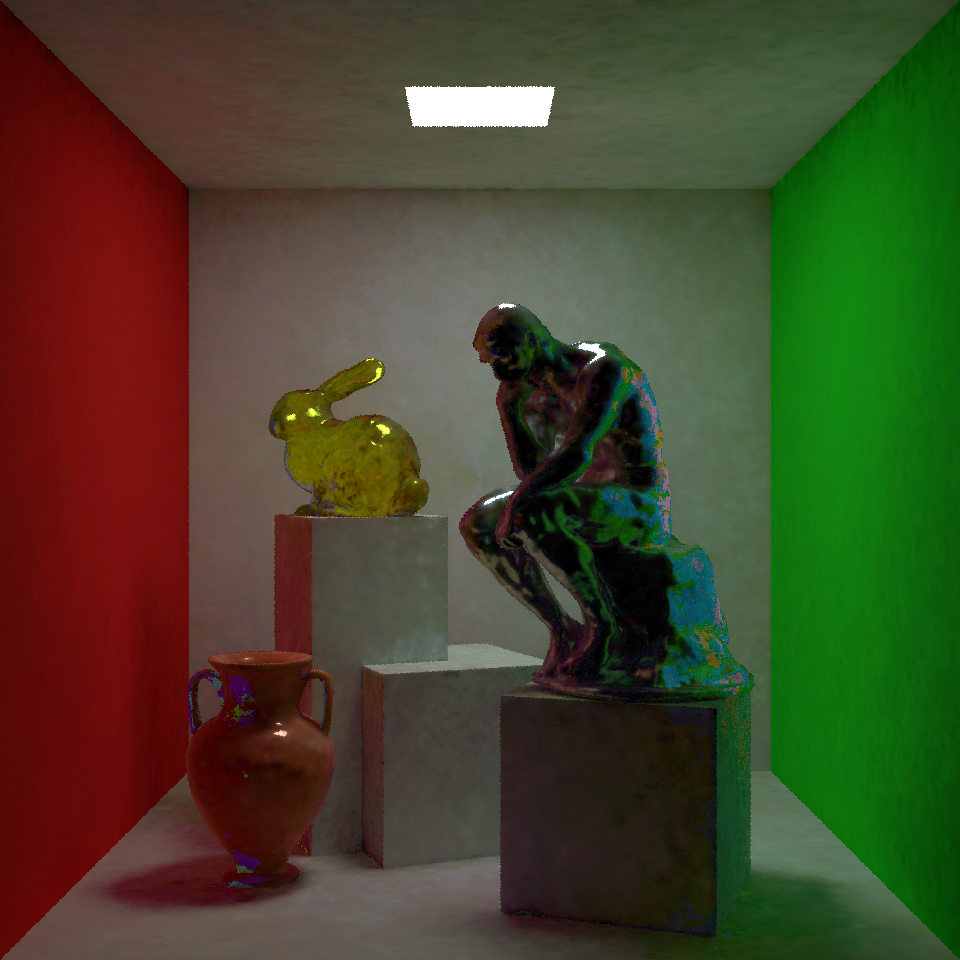
\includegraphics[width=\linewidth]{figures/py/tests/path_termination/1stvert_1spp_thinker.png}
\\
&& 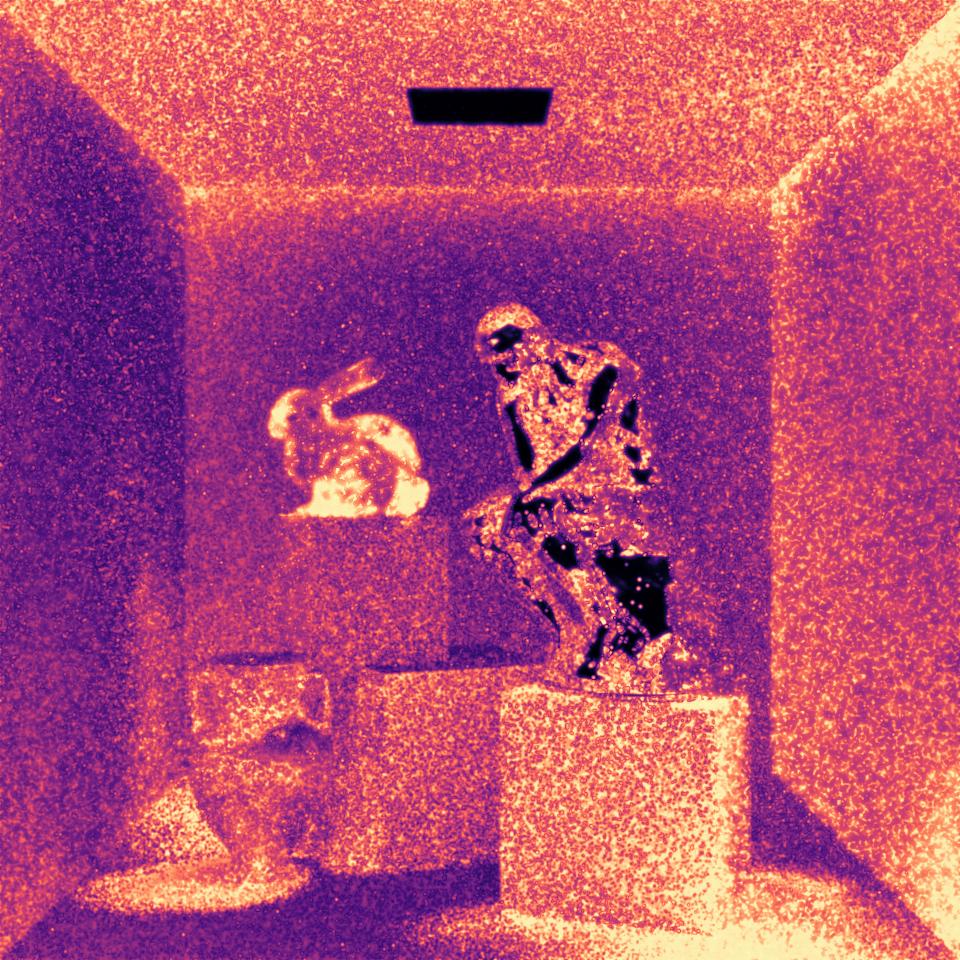
\includegraphics[width=\linewidth]{figures/py/tests/path_termination/ref_1spp_thinker_flip.png}
& 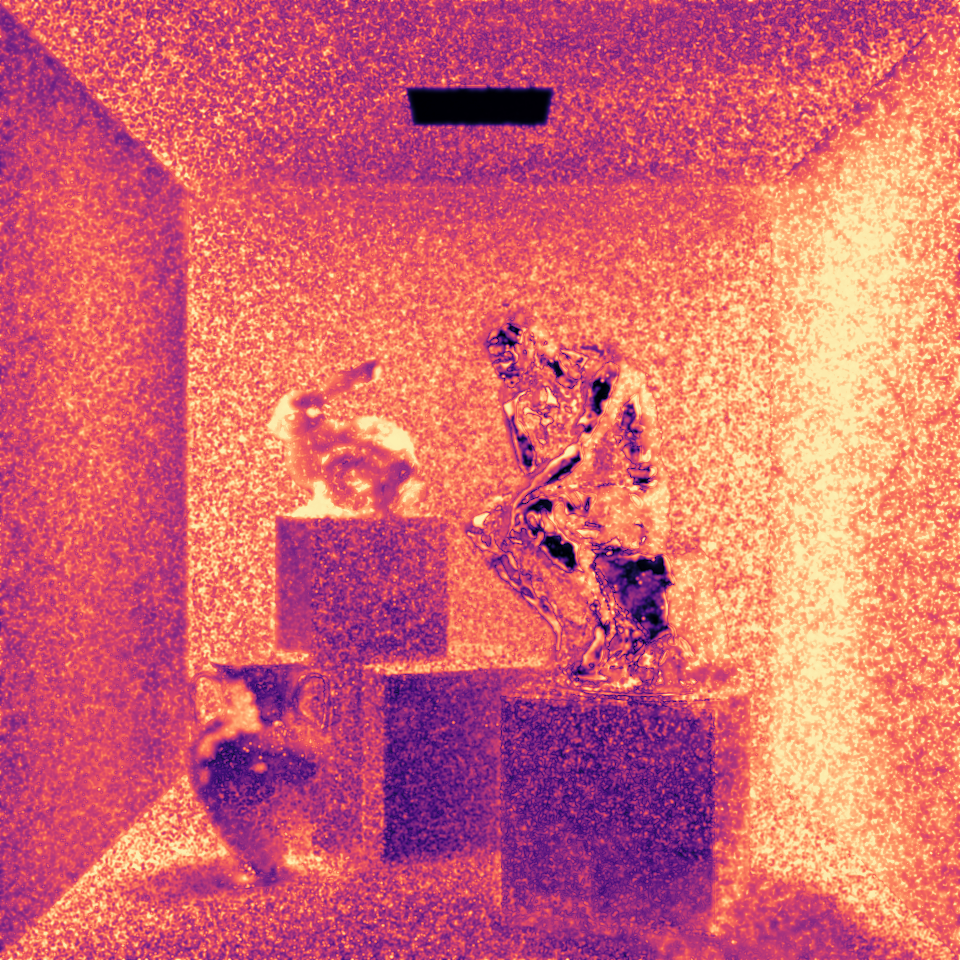
\includegraphics[width=\linewidth]{figures/py/tests/path_termination/sah_1spp_thinker_flip.png}
& 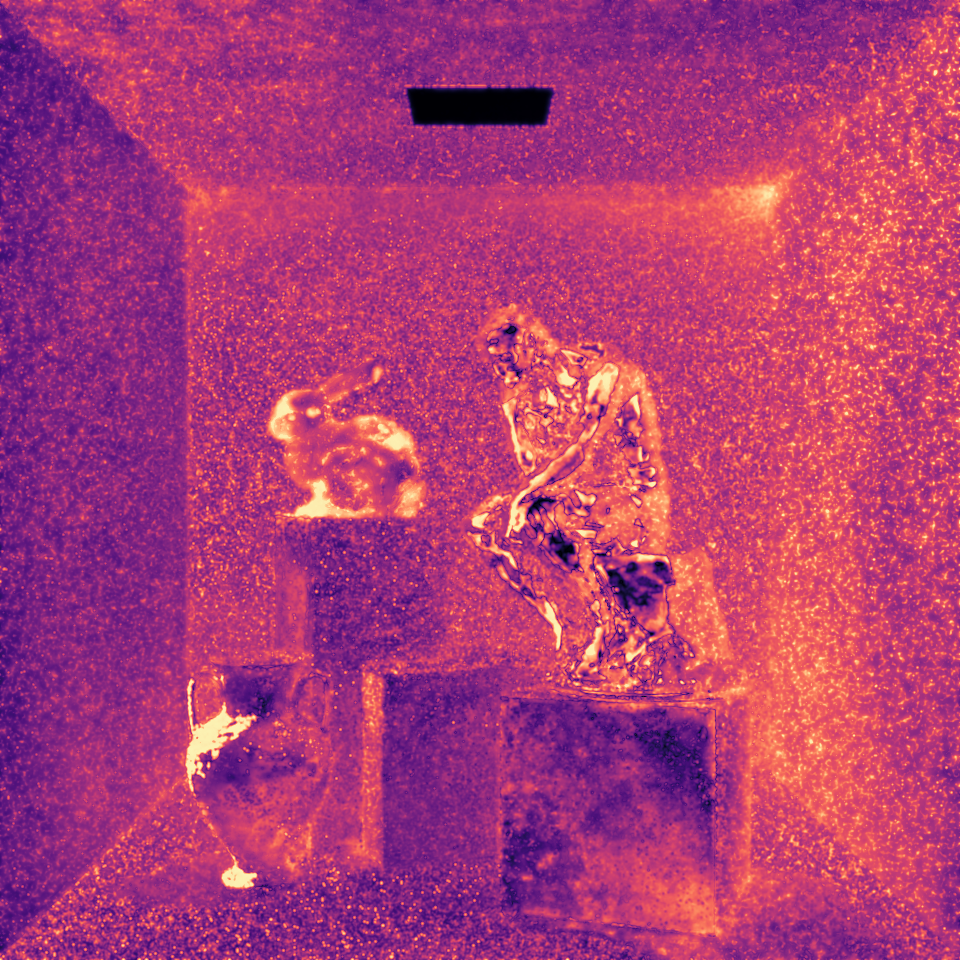
\includegraphics[width=\linewidth]{figures/py/tests/path_termination/bth_1spp_thinker_flip.png}
& 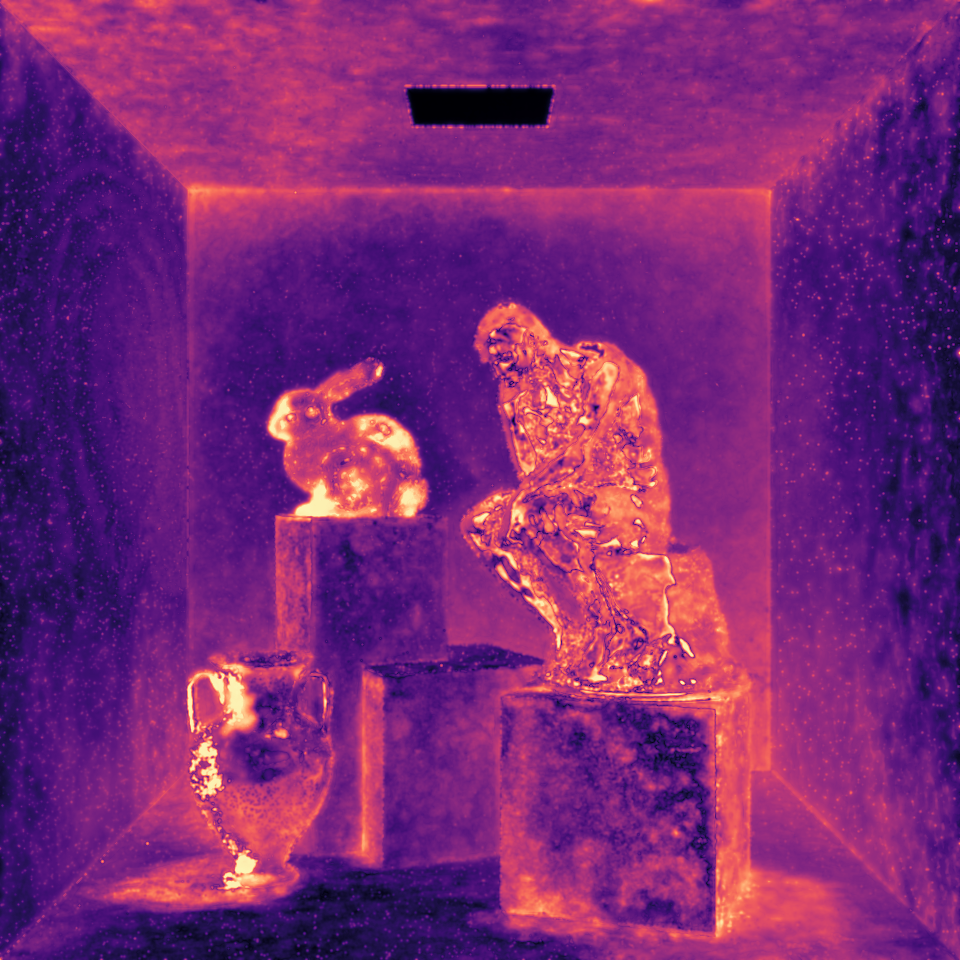
\includegraphics[width=\linewidth]{figures/py/tests/path_termination/bthk9_1spp_thinker_flip.png}
& 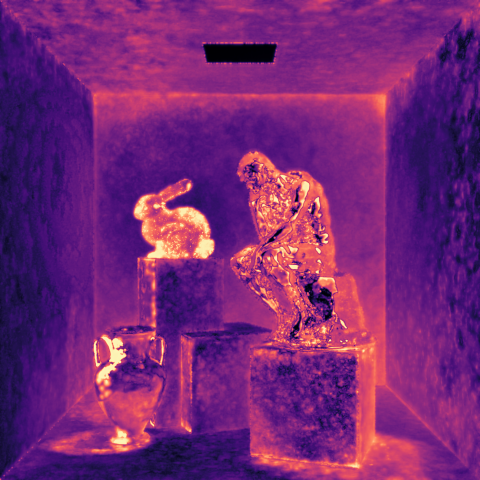
\includegraphics[width=\linewidth]{figures/py/tests/path_termination/1stdiff_1spp_thinker_flip.png}
& 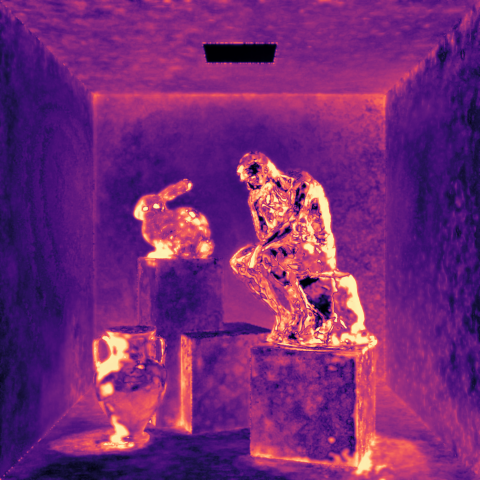
\includegraphics[width=\linewidth]{figures/py/tests/path_termination/1stvert_1spp_thinker_flip.png}
\\
&\FLIP/MSE: & \num{0.531}/\num{0.061}
 & \num{0.633}/\num{0.335}
 & \num{0.491}/\num{0.206}
 & \num{0.360}/\num{0.013}
 & \textbf{\num{0.351}}/\num{0.014}
 & \num{0.355}/\textbf{\num{0.011}}
\\
&$\mathrm{Bias}^2/\mathrm{Variance}$ & \textbf{\num{6.42e-09}}/\num{6.38e-02}
 & \num{5.29e-05}/\num{2.77e-01}
 & \num{1.23e-04}/\num{1.31e-01}
 & \num{1.46e-04}/\num{1.47e-02}
 & \num{1.43e-04}/\num{1.48e-02}
 & \num{1.40e-04}/\textbf{\num{8.81e-03}}
\\

    \end{tabularx}
    \caption{Comparison of the Path Termination strategies from \autoref{sec:path_termination}.}
    \label{fig:pathterm_comparison}
\end{figure}

\paragraph{Next Event Estimation}

\section{Training}

\begin{figure}[ht]
    \centering
    %% Creator: Matplotlib, PGF backend
%%
%% To include the figure in your LaTeX document, write
%%   \input{<filename>.pgf}
%%
%% Make sure the required packages are loaded in your preamble
%%   \usepackage{pgf}
%%
%% Also ensure that all the required font packages are loaded; for instance,
%% the lmodern package is sometimes necessary when using math font.
%%   \usepackage{lmodern}
%%
%% Figures using additional raster images can only be included by \input if
%% they are in the same directory as the main LaTeX file. For loading figures
%% from other directories you can use the `import` package
%%   \usepackage{import}
%%
%% and then include the figures with
%%   \import{<path to file>}{<filename>.pgf}
%%
%% Matplotlib used the following preamble
%%   \def\mathdefault#1{#1}
%%   \everymath=\expandafter{\the\everymath\displaystyle}
%%   \IfFileExists{scrextend.sty}{
%%     \usepackage[fontsize=6.000000pt]{scrextend}
%%   }{
%%     \renewcommand{\normalsize}{\fontsize{6.000000}{7.200000}\selectfont}
%%     \normalsize
%%   }
%%   
%%   \ifdefined\pdftexversion\else  % non-pdftex case.
%%     \usepackage{fontspec}
%%     \setmainfont{DejaVuSerif.ttf}[Path=\detokenize{/opt/homebrew/Cellar/python-matplotlib/3.10.5/libexec/lib/python3.13/site-packages/matplotlib/mpl-data/fonts/ttf/}]
%%     \setsansfont{DejaVuSans.ttf}[Path=\detokenize{/opt/homebrew/Cellar/python-matplotlib/3.10.5/libexec/lib/python3.13/site-packages/matplotlib/mpl-data/fonts/ttf/}]
%%     \setmonofont{DejaVuSansMono.ttf}[Path=\detokenize{/opt/homebrew/Cellar/python-matplotlib/3.10.5/libexec/lib/python3.13/site-packages/matplotlib/mpl-data/fonts/ttf/}]
%%   \fi
%%   \makeatletter\@ifpackageloaded{underscore}{}{\usepackage[strings]{underscore}}\makeatother
%%
\begingroup%
\makeatletter%
\begin{pgfpicture}%
\pgfpathrectangle{\pgfpointorigin}{\pgfqpoint{6.684351in}{1.284073in}}%
\pgfusepath{use as bounding box, clip}%
\begin{pgfscope}%
\pgfsetbuttcap%
\pgfsetmiterjoin%
\definecolor{currentfill}{rgb}{1.000000,1.000000,1.000000}%
\pgfsetfillcolor{currentfill}%
\pgfsetlinewidth{0.000000pt}%
\definecolor{currentstroke}{rgb}{1.000000,1.000000,1.000000}%
\pgfsetstrokecolor{currentstroke}%
\pgfsetdash{}{0pt}%
\pgfpathmoveto{\pgfqpoint{0.000000in}{0.000000in}}%
\pgfpathlineto{\pgfqpoint{6.684351in}{0.000000in}}%
\pgfpathlineto{\pgfqpoint{6.684351in}{1.284073in}}%
\pgfpathlineto{\pgfqpoint{0.000000in}{1.284073in}}%
\pgfpathlineto{\pgfqpoint{0.000000in}{0.000000in}}%
\pgfpathclose%
\pgfusepath{fill}%
\end{pgfscope}%
\begin{pgfscope}%
\pgfsetbuttcap%
\pgfsetmiterjoin%
\definecolor{currentfill}{rgb}{1.000000,1.000000,1.000000}%
\pgfsetfillcolor{currentfill}%
\pgfsetlinewidth{0.000000pt}%
\definecolor{currentstroke}{rgb}{0.000000,0.000000,0.000000}%
\pgfsetstrokecolor{currentstroke}%
\pgfsetstrokeopacity{0.000000}%
\pgfsetdash{}{0pt}%
\pgfpathmoveto{\pgfqpoint{0.384351in}{0.414073in}}%
\pgfpathlineto{\pgfqpoint{6.584351in}{0.414073in}}%
\pgfpathlineto{\pgfqpoint{6.584351in}{1.184073in}}%
\pgfpathlineto{\pgfqpoint{0.384351in}{1.184073in}}%
\pgfpathlineto{\pgfqpoint{0.384351in}{0.414073in}}%
\pgfpathclose%
\pgfusepath{fill}%
\end{pgfscope}%
\begin{pgfscope}%
\pgfsetbuttcap%
\pgfsetroundjoin%
\definecolor{currentfill}{rgb}{0.000000,0.000000,0.000000}%
\pgfsetfillcolor{currentfill}%
\pgfsetlinewidth{0.803000pt}%
\definecolor{currentstroke}{rgb}{0.000000,0.000000,0.000000}%
\pgfsetstrokecolor{currentstroke}%
\pgfsetdash{}{0pt}%
\pgfsys@defobject{currentmarker}{\pgfqpoint{0.000000in}{-0.048611in}}{\pgfqpoint{0.000000in}{0.000000in}}{%
\pgfpathmoveto{\pgfqpoint{0.000000in}{0.000000in}}%
\pgfpathlineto{\pgfqpoint{0.000000in}{-0.048611in}}%
\pgfusepath{stroke,fill}%
}%
\begin{pgfscope}%
\pgfsys@transformshift{0.384351in}{0.414073in}%
\pgfsys@useobject{currentmarker}{}%
\end{pgfscope}%
\end{pgfscope}%
\begin{pgfscope}%
\definecolor{textcolor}{rgb}{0.000000,0.000000,0.000000}%
\pgfsetstrokecolor{textcolor}%
\pgfsetfillcolor{textcolor}%
\pgftext[x=0.384351in,y=0.316851in,,top]{\color{textcolor}{\rmfamily\fontsize{6.000000}{7.200000}\selectfont\catcode`\^=\active\def^{\ifmmode\sp\else\^{}\fi}\catcode`\%=\active\def%{\%}$\mathdefault{0}$}}%
\end{pgfscope}%
\begin{pgfscope}%
\pgfsetbuttcap%
\pgfsetroundjoin%
\definecolor{currentfill}{rgb}{0.000000,0.000000,0.000000}%
\pgfsetfillcolor{currentfill}%
\pgfsetlinewidth{0.803000pt}%
\definecolor{currentstroke}{rgb}{0.000000,0.000000,0.000000}%
\pgfsetstrokecolor{currentstroke}%
\pgfsetdash{}{0pt}%
\pgfsys@defobject{currentmarker}{\pgfqpoint{0.000000in}{-0.048611in}}{\pgfqpoint{0.000000in}{0.000000in}}{%
\pgfpathmoveto{\pgfqpoint{0.000000in}{0.000000in}}%
\pgfpathlineto{\pgfqpoint{0.000000in}{-0.048611in}}%
\pgfusepath{stroke,fill}%
}%
\begin{pgfscope}%
\pgfsys@transformshift{1.724819in}{0.414073in}%
\pgfsys@useobject{currentmarker}{}%
\end{pgfscope}%
\end{pgfscope}%
\begin{pgfscope}%
\definecolor{textcolor}{rgb}{0.000000,0.000000,0.000000}%
\pgfsetstrokecolor{textcolor}%
\pgfsetfillcolor{textcolor}%
\pgftext[x=1.724819in,y=0.316851in,,top]{\color{textcolor}{\rmfamily\fontsize{6.000000}{7.200000}\selectfont\catcode`\^=\active\def^{\ifmmode\sp\else\^{}\fi}\catcode`\%=\active\def%{\%}$\mathdefault{200}$}}%
\end{pgfscope}%
\begin{pgfscope}%
\pgfsetbuttcap%
\pgfsetroundjoin%
\definecolor{currentfill}{rgb}{0.000000,0.000000,0.000000}%
\pgfsetfillcolor{currentfill}%
\pgfsetlinewidth{0.803000pt}%
\definecolor{currentstroke}{rgb}{0.000000,0.000000,0.000000}%
\pgfsetstrokecolor{currentstroke}%
\pgfsetdash{}{0pt}%
\pgfsys@defobject{currentmarker}{\pgfqpoint{0.000000in}{-0.048611in}}{\pgfqpoint{0.000000in}{0.000000in}}{%
\pgfpathmoveto{\pgfqpoint{0.000000in}{0.000000in}}%
\pgfpathlineto{\pgfqpoint{0.000000in}{-0.048611in}}%
\pgfusepath{stroke,fill}%
}%
\begin{pgfscope}%
\pgfsys@transformshift{3.065287in}{0.414073in}%
\pgfsys@useobject{currentmarker}{}%
\end{pgfscope}%
\end{pgfscope}%
\begin{pgfscope}%
\definecolor{textcolor}{rgb}{0.000000,0.000000,0.000000}%
\pgfsetstrokecolor{textcolor}%
\pgfsetfillcolor{textcolor}%
\pgftext[x=3.065287in,y=0.316851in,,top]{\color{textcolor}{\rmfamily\fontsize{6.000000}{7.200000}\selectfont\catcode`\^=\active\def^{\ifmmode\sp\else\^{}\fi}\catcode`\%=\active\def%{\%}$\mathdefault{400}$}}%
\end{pgfscope}%
\begin{pgfscope}%
\pgfsetbuttcap%
\pgfsetroundjoin%
\definecolor{currentfill}{rgb}{0.000000,0.000000,0.000000}%
\pgfsetfillcolor{currentfill}%
\pgfsetlinewidth{0.803000pt}%
\definecolor{currentstroke}{rgb}{0.000000,0.000000,0.000000}%
\pgfsetstrokecolor{currentstroke}%
\pgfsetdash{}{0pt}%
\pgfsys@defobject{currentmarker}{\pgfqpoint{0.000000in}{-0.048611in}}{\pgfqpoint{0.000000in}{0.000000in}}{%
\pgfpathmoveto{\pgfqpoint{0.000000in}{0.000000in}}%
\pgfpathlineto{\pgfqpoint{0.000000in}{-0.048611in}}%
\pgfusepath{stroke,fill}%
}%
\begin{pgfscope}%
\pgfsys@transformshift{4.405755in}{0.414073in}%
\pgfsys@useobject{currentmarker}{}%
\end{pgfscope}%
\end{pgfscope}%
\begin{pgfscope}%
\definecolor{textcolor}{rgb}{0.000000,0.000000,0.000000}%
\pgfsetstrokecolor{textcolor}%
\pgfsetfillcolor{textcolor}%
\pgftext[x=4.405755in,y=0.316851in,,top]{\color{textcolor}{\rmfamily\fontsize{6.000000}{7.200000}\selectfont\catcode`\^=\active\def^{\ifmmode\sp\else\^{}\fi}\catcode`\%=\active\def%{\%}$\mathdefault{600}$}}%
\end{pgfscope}%
\begin{pgfscope}%
\pgfsetbuttcap%
\pgfsetroundjoin%
\definecolor{currentfill}{rgb}{0.000000,0.000000,0.000000}%
\pgfsetfillcolor{currentfill}%
\pgfsetlinewidth{0.803000pt}%
\definecolor{currentstroke}{rgb}{0.000000,0.000000,0.000000}%
\pgfsetstrokecolor{currentstroke}%
\pgfsetdash{}{0pt}%
\pgfsys@defobject{currentmarker}{\pgfqpoint{0.000000in}{-0.048611in}}{\pgfqpoint{0.000000in}{0.000000in}}{%
\pgfpathmoveto{\pgfqpoint{0.000000in}{0.000000in}}%
\pgfpathlineto{\pgfqpoint{0.000000in}{-0.048611in}}%
\pgfusepath{stroke,fill}%
}%
\begin{pgfscope}%
\pgfsys@transformshift{5.746223in}{0.414073in}%
\pgfsys@useobject{currentmarker}{}%
\end{pgfscope}%
\end{pgfscope}%
\begin{pgfscope}%
\definecolor{textcolor}{rgb}{0.000000,0.000000,0.000000}%
\pgfsetstrokecolor{textcolor}%
\pgfsetfillcolor{textcolor}%
\pgftext[x=5.746223in,y=0.316851in,,top]{\color{textcolor}{\rmfamily\fontsize{6.000000}{7.200000}\selectfont\catcode`\^=\active\def^{\ifmmode\sp\else\^{}\fi}\catcode`\%=\active\def%{\%}$\mathdefault{800}$}}%
\end{pgfscope}%
\begin{pgfscope}%
\definecolor{textcolor}{rgb}{0.000000,0.000000,0.000000}%
\pgfsetstrokecolor{textcolor}%
\pgfsetfillcolor{textcolor}%
\pgftext[x=3.484351in,y=0.180648in,,top]{\color{textcolor}{\rmfamily\fontsize{6.000000}{7.200000}\selectfont\catcode`\^=\active\def^{\ifmmode\sp\else\^{}\fi}\catcode`\%=\active\def%{\%}Iterations}}%
\end{pgfscope}%
\begin{pgfscope}%
\pgfsetbuttcap%
\pgfsetroundjoin%
\definecolor{currentfill}{rgb}{0.000000,0.000000,0.000000}%
\pgfsetfillcolor{currentfill}%
\pgfsetlinewidth{0.803000pt}%
\definecolor{currentstroke}{rgb}{0.000000,0.000000,0.000000}%
\pgfsetstrokecolor{currentstroke}%
\pgfsetdash{}{0pt}%
\pgfsys@defobject{currentmarker}{\pgfqpoint{-0.048611in}{0.000000in}}{\pgfqpoint{-0.000000in}{0.000000in}}{%
\pgfpathmoveto{\pgfqpoint{-0.000000in}{0.000000in}}%
\pgfpathlineto{\pgfqpoint{-0.048611in}{0.000000in}}%
\pgfusepath{stroke,fill}%
}%
\begin{pgfscope}%
\pgfsys@transformshift{0.384351in}{0.414073in}%
\pgfsys@useobject{currentmarker}{}%
\end{pgfscope}%
\end{pgfscope}%
\begin{pgfscope}%
\definecolor{textcolor}{rgb}{0.000000,0.000000,0.000000}%
\pgfsetstrokecolor{textcolor}%
\pgfsetfillcolor{textcolor}%
\pgftext[x=0.236203in, y=0.382416in, left, base]{\color{textcolor}{\rmfamily\fontsize{6.000000}{7.200000}\selectfont\catcode`\^=\active\def^{\ifmmode\sp\else\^{}\fi}\catcode`\%=\active\def%{\%}$\mathdefault{0}$}}%
\end{pgfscope}%
\begin{pgfscope}%
\pgfsetbuttcap%
\pgfsetroundjoin%
\definecolor{currentfill}{rgb}{0.000000,0.000000,0.000000}%
\pgfsetfillcolor{currentfill}%
\pgfsetlinewidth{0.803000pt}%
\definecolor{currentstroke}{rgb}{0.000000,0.000000,0.000000}%
\pgfsetstrokecolor{currentstroke}%
\pgfsetdash{}{0pt}%
\pgfsys@defobject{currentmarker}{\pgfqpoint{-0.048611in}{0.000000in}}{\pgfqpoint{-0.000000in}{0.000000in}}{%
\pgfpathmoveto{\pgfqpoint{-0.000000in}{0.000000in}}%
\pgfpathlineto{\pgfqpoint{-0.048611in}{0.000000in}}%
\pgfusepath{stroke,fill}%
}%
\begin{pgfscope}%
\pgfsys@transformshift{0.384351in}{0.722073in}%
\pgfsys@useobject{currentmarker}{}%
\end{pgfscope}%
\end{pgfscope}%
\begin{pgfscope}%
\definecolor{textcolor}{rgb}{0.000000,0.000000,0.000000}%
\pgfsetstrokecolor{textcolor}%
\pgfsetfillcolor{textcolor}%
\pgftext[x=0.236203in, y=0.690416in, left, base]{\color{textcolor}{\rmfamily\fontsize{6.000000}{7.200000}\selectfont\catcode`\^=\active\def^{\ifmmode\sp\else\^{}\fi}\catcode`\%=\active\def%{\%}$\mathdefault{2}$}}%
\end{pgfscope}%
\begin{pgfscope}%
\pgfsetbuttcap%
\pgfsetroundjoin%
\definecolor{currentfill}{rgb}{0.000000,0.000000,0.000000}%
\pgfsetfillcolor{currentfill}%
\pgfsetlinewidth{0.803000pt}%
\definecolor{currentstroke}{rgb}{0.000000,0.000000,0.000000}%
\pgfsetstrokecolor{currentstroke}%
\pgfsetdash{}{0pt}%
\pgfsys@defobject{currentmarker}{\pgfqpoint{-0.048611in}{0.000000in}}{\pgfqpoint{-0.000000in}{0.000000in}}{%
\pgfpathmoveto{\pgfqpoint{-0.000000in}{0.000000in}}%
\pgfpathlineto{\pgfqpoint{-0.048611in}{0.000000in}}%
\pgfusepath{stroke,fill}%
}%
\begin{pgfscope}%
\pgfsys@transformshift{0.384351in}{1.030073in}%
\pgfsys@useobject{currentmarker}{}%
\end{pgfscope}%
\end{pgfscope}%
\begin{pgfscope}%
\definecolor{textcolor}{rgb}{0.000000,0.000000,0.000000}%
\pgfsetstrokecolor{textcolor}%
\pgfsetfillcolor{textcolor}%
\pgftext[x=0.236203in, y=0.998416in, left, base]{\color{textcolor}{\rmfamily\fontsize{6.000000}{7.200000}\selectfont\catcode`\^=\active\def^{\ifmmode\sp\else\^{}\fi}\catcode`\%=\active\def%{\%}$\mathdefault{4}$}}%
\end{pgfscope}%
\begin{pgfscope}%
\definecolor{textcolor}{rgb}{0.000000,0.000000,0.000000}%
\pgfsetstrokecolor{textcolor}%
\pgfsetfillcolor{textcolor}%
\pgftext[x=0.180648in,y=0.799073in,,bottom,rotate=90.000000]{\color{textcolor}{\rmfamily\fontsize{6.000000}{7.200000}\selectfont\catcode`\^=\active\def^{\ifmmode\sp\else\^{}\fi}\catcode`\%=\active\def%{\%}Relative L2 Loss}}%
\end{pgfscope}%
\begin{pgfscope}%
\pgfpathrectangle{\pgfqpoint{0.384351in}{0.414073in}}{\pgfqpoint{6.200000in}{0.770000in}}%
\pgfusepath{clip}%
\pgfsetrectcap%
\pgfsetroundjoin%
\pgfsetlinewidth{1.505625pt}%
\definecolor{currentstroke}{rgb}{0.121569,0.466667,0.705882}%
\pgfsetstrokecolor{currentstroke}%
\pgfsetdash{}{0pt}%
\pgfpathmoveto{\pgfqpoint{0.384351in}{0.858591in}}%
\pgfpathlineto{\pgfqpoint{0.391053in}{1.041250in}}%
\pgfpathlineto{\pgfqpoint{0.397755in}{0.525196in}}%
\pgfpathlineto{\pgfqpoint{0.404458in}{0.493575in}}%
\pgfpathlineto{\pgfqpoint{0.411160in}{0.489410in}}%
\pgfpathlineto{\pgfqpoint{0.417862in}{0.486660in}}%
\pgfpathlineto{\pgfqpoint{0.424565in}{0.488265in}}%
\pgfpathlineto{\pgfqpoint{0.431267in}{0.505424in}}%
\pgfpathlineto{\pgfqpoint{0.437969in}{0.533593in}}%
\pgfpathlineto{\pgfqpoint{0.444672in}{0.539595in}}%
\pgfpathlineto{\pgfqpoint{0.451374in}{0.526369in}}%
\pgfpathlineto{\pgfqpoint{0.458076in}{0.501888in}}%
\pgfpathlineto{\pgfqpoint{0.464779in}{0.484166in}}%
\pgfpathlineto{\pgfqpoint{0.471481in}{0.473969in}}%
\pgfpathlineto{\pgfqpoint{0.478183in}{0.468221in}}%
\pgfpathlineto{\pgfqpoint{0.484886in}{0.465341in}}%
\pgfpathlineto{\pgfqpoint{0.491588in}{0.464095in}}%
\pgfpathlineto{\pgfqpoint{0.498290in}{0.464978in}}%
\pgfpathlineto{\pgfqpoint{0.511695in}{0.473483in}}%
\pgfpathlineto{\pgfqpoint{0.518397in}{0.477816in}}%
\pgfpathlineto{\pgfqpoint{0.525100in}{0.479467in}}%
\pgfpathlineto{\pgfqpoint{0.531802in}{0.479169in}}%
\pgfpathlineto{\pgfqpoint{0.538504in}{0.476593in}}%
\pgfpathlineto{\pgfqpoint{0.545207in}{0.470927in}}%
\pgfpathlineto{\pgfqpoint{0.551909in}{0.473928in}}%
\pgfpathlineto{\pgfqpoint{0.558611in}{0.480181in}}%
\pgfpathlineto{\pgfqpoint{0.572016in}{0.473886in}}%
\pgfpathlineto{\pgfqpoint{0.578718in}{0.478284in}}%
\pgfpathlineto{\pgfqpoint{0.585421in}{0.476691in}}%
\pgfpathlineto{\pgfqpoint{0.592123in}{0.470697in}}%
\pgfpathlineto{\pgfqpoint{0.598825in}{0.468470in}}%
\pgfpathlineto{\pgfqpoint{0.612230in}{0.468626in}}%
\pgfpathlineto{\pgfqpoint{0.625635in}{0.466256in}}%
\pgfpathlineto{\pgfqpoint{0.632337in}{0.466167in}}%
\pgfpathlineto{\pgfqpoint{0.645742in}{0.462351in}}%
\pgfpathlineto{\pgfqpoint{0.652444in}{0.464198in}}%
\pgfpathlineto{\pgfqpoint{0.659147in}{0.464180in}}%
\pgfpathlineto{\pgfqpoint{0.672551in}{0.467851in}}%
\pgfpathlineto{\pgfqpoint{0.692658in}{0.463258in}}%
\pgfpathlineto{\pgfqpoint{0.699361in}{0.462425in}}%
\pgfpathlineto{\pgfqpoint{0.706063in}{0.459657in}}%
\pgfpathlineto{\pgfqpoint{0.712765in}{0.461603in}}%
\pgfpathlineto{\pgfqpoint{0.719468in}{0.462312in}}%
\pgfpathlineto{\pgfqpoint{0.726170in}{0.460721in}}%
\pgfpathlineto{\pgfqpoint{0.732872in}{0.460332in}}%
\pgfpathlineto{\pgfqpoint{0.739575in}{0.458736in}}%
\pgfpathlineto{\pgfqpoint{0.746277in}{0.458642in}}%
\pgfpathlineto{\pgfqpoint{0.752979in}{0.459736in}}%
\pgfpathlineto{\pgfqpoint{0.759682in}{0.462581in}}%
\pgfpathlineto{\pgfqpoint{0.766384in}{0.462707in}}%
\pgfpathlineto{\pgfqpoint{0.773086in}{0.460186in}}%
\pgfpathlineto{\pgfqpoint{0.786491in}{0.459064in}}%
\pgfpathlineto{\pgfqpoint{0.799896in}{0.458820in}}%
\pgfpathlineto{\pgfqpoint{0.806598in}{0.460489in}}%
\pgfpathlineto{\pgfqpoint{0.820003in}{0.458703in}}%
\pgfpathlineto{\pgfqpoint{0.826705in}{0.463528in}}%
\pgfpathlineto{\pgfqpoint{0.833407in}{0.463041in}}%
\pgfpathlineto{\pgfqpoint{0.840110in}{0.458570in}}%
\pgfpathlineto{\pgfqpoint{0.846812in}{0.458670in}}%
\pgfpathlineto{\pgfqpoint{0.860217in}{0.466084in}}%
\pgfpathlineto{\pgfqpoint{0.866919in}{0.462732in}}%
\pgfpathlineto{\pgfqpoint{0.873621in}{0.457615in}}%
\pgfpathlineto{\pgfqpoint{0.893728in}{0.459826in}}%
\pgfpathlineto{\pgfqpoint{0.900431in}{0.458059in}}%
\pgfpathlineto{\pgfqpoint{0.907133in}{0.458052in}}%
\pgfpathlineto{\pgfqpoint{0.913835in}{0.460039in}}%
\pgfpathlineto{\pgfqpoint{0.927240in}{0.457874in}}%
\pgfpathlineto{\pgfqpoint{0.933942in}{0.458948in}}%
\pgfpathlineto{\pgfqpoint{0.940645in}{0.457122in}}%
\pgfpathlineto{\pgfqpoint{0.947347in}{0.456720in}}%
\pgfpathlineto{\pgfqpoint{0.967454in}{0.459941in}}%
\pgfpathlineto{\pgfqpoint{0.974157in}{0.458829in}}%
\pgfpathlineto{\pgfqpoint{0.980859in}{0.459827in}}%
\pgfpathlineto{\pgfqpoint{0.987561in}{0.464278in}}%
\pgfpathlineto{\pgfqpoint{0.994264in}{0.462460in}}%
\pgfpathlineto{\pgfqpoint{1.000966in}{0.459158in}}%
\pgfpathlineto{\pgfqpoint{1.014371in}{0.461676in}}%
\pgfpathlineto{\pgfqpoint{1.021073in}{0.460581in}}%
\pgfpathlineto{\pgfqpoint{1.027775in}{0.462280in}}%
\pgfpathlineto{\pgfqpoint{1.034478in}{0.462022in}}%
\pgfpathlineto{\pgfqpoint{1.041180in}{0.457905in}}%
\pgfpathlineto{\pgfqpoint{1.067989in}{0.456956in}}%
\pgfpathlineto{\pgfqpoint{1.081394in}{0.457242in}}%
\pgfpathlineto{\pgfqpoint{1.088096in}{0.459460in}}%
\pgfpathlineto{\pgfqpoint{1.108203in}{0.457242in}}%
\pgfpathlineto{\pgfqpoint{1.114906in}{0.458740in}}%
\pgfpathlineto{\pgfqpoint{1.141715in}{0.457072in}}%
\pgfpathlineto{\pgfqpoint{1.148417in}{0.458470in}}%
\pgfpathlineto{\pgfqpoint{1.168524in}{0.456988in}}%
\pgfpathlineto{\pgfqpoint{1.181929in}{0.460408in}}%
\pgfpathlineto{\pgfqpoint{1.188631in}{0.457690in}}%
\pgfpathlineto{\pgfqpoint{1.195334in}{0.459433in}}%
\pgfpathlineto{\pgfqpoint{1.208738in}{0.460795in}}%
\pgfpathlineto{\pgfqpoint{1.215441in}{0.463660in}}%
\pgfpathlineto{\pgfqpoint{1.222143in}{0.458242in}}%
\pgfpathlineto{\pgfqpoint{1.228845in}{0.457483in}}%
\pgfpathlineto{\pgfqpoint{1.235548in}{0.460998in}}%
\pgfpathlineto{\pgfqpoint{1.242250in}{0.458831in}}%
\pgfpathlineto{\pgfqpoint{1.248952in}{0.460989in}}%
\pgfpathlineto{\pgfqpoint{1.255655in}{0.461065in}}%
\pgfpathlineto{\pgfqpoint{1.262357in}{0.456031in}}%
\pgfpathlineto{\pgfqpoint{1.275762in}{0.458618in}}%
\pgfpathlineto{\pgfqpoint{1.289167in}{0.456524in}}%
\pgfpathlineto{\pgfqpoint{1.302571in}{0.460004in}}%
\pgfpathlineto{\pgfqpoint{1.315976in}{0.455406in}}%
\pgfpathlineto{\pgfqpoint{1.329381in}{0.455938in}}%
\pgfpathlineto{\pgfqpoint{1.336083in}{0.456106in}}%
\pgfpathlineto{\pgfqpoint{1.342785in}{0.460419in}}%
\pgfpathlineto{\pgfqpoint{1.349488in}{0.459679in}}%
\pgfpathlineto{\pgfqpoint{1.356190in}{0.456462in}}%
\pgfpathlineto{\pgfqpoint{1.362892in}{0.456936in}}%
\pgfpathlineto{\pgfqpoint{1.382999in}{0.455729in}}%
\pgfpathlineto{\pgfqpoint{1.403106in}{0.454941in}}%
\pgfpathlineto{\pgfqpoint{1.416511in}{0.461404in}}%
\pgfpathlineto{\pgfqpoint{1.423213in}{0.458425in}}%
\pgfpathlineto{\pgfqpoint{1.429916in}{0.456678in}}%
\pgfpathlineto{\pgfqpoint{1.436618in}{0.458069in}}%
\pgfpathlineto{\pgfqpoint{1.443320in}{0.455602in}}%
\pgfpathlineto{\pgfqpoint{1.470130in}{0.457890in}}%
\pgfpathlineto{\pgfqpoint{1.476832in}{0.460847in}}%
\pgfpathlineto{\pgfqpoint{1.483534in}{0.459704in}}%
\pgfpathlineto{\pgfqpoint{1.490237in}{0.456427in}}%
\pgfpathlineto{\pgfqpoint{1.503641in}{0.455063in}}%
\pgfpathlineto{\pgfqpoint{1.510344in}{0.456604in}}%
\pgfpathlineto{\pgfqpoint{1.517046in}{0.466143in}}%
\pgfpathlineto{\pgfqpoint{1.523748in}{0.464699in}}%
\pgfpathlineto{\pgfqpoint{1.530451in}{0.456732in}}%
\pgfpathlineto{\pgfqpoint{1.550558in}{0.455998in}}%
\pgfpathlineto{\pgfqpoint{1.557260in}{0.457584in}}%
\pgfpathlineto{\pgfqpoint{1.570665in}{0.455465in}}%
\pgfpathlineto{\pgfqpoint{1.577367in}{0.456705in}}%
\pgfpathlineto{\pgfqpoint{1.584069in}{0.455763in}}%
\pgfpathlineto{\pgfqpoint{1.597474in}{0.457635in}}%
\pgfpathlineto{\pgfqpoint{1.604177in}{0.456547in}}%
\pgfpathlineto{\pgfqpoint{1.610879in}{0.457987in}}%
\pgfpathlineto{\pgfqpoint{1.617581in}{0.462584in}}%
\pgfpathlineto{\pgfqpoint{1.624284in}{0.465016in}}%
\pgfpathlineto{\pgfqpoint{1.637688in}{0.457885in}}%
\pgfpathlineto{\pgfqpoint{1.644391in}{0.456342in}}%
\pgfpathlineto{\pgfqpoint{1.651093in}{0.457718in}}%
\pgfpathlineto{\pgfqpoint{1.664498in}{0.454256in}}%
\pgfpathlineto{\pgfqpoint{1.671200in}{0.455812in}}%
\pgfpathlineto{\pgfqpoint{1.684605in}{0.453922in}}%
\pgfpathlineto{\pgfqpoint{1.691307in}{0.455866in}}%
\pgfpathlineto{\pgfqpoint{1.698009in}{0.462540in}}%
\pgfpathlineto{\pgfqpoint{1.724819in}{0.456168in}}%
\pgfpathlineto{\pgfqpoint{1.731521in}{0.457281in}}%
\pgfpathlineto{\pgfqpoint{1.738223in}{0.455780in}}%
\pgfpathlineto{\pgfqpoint{1.744926in}{0.460570in}}%
\pgfpathlineto{\pgfqpoint{1.751628in}{0.460668in}}%
\pgfpathlineto{\pgfqpoint{1.758330in}{0.454883in}}%
\pgfpathlineto{\pgfqpoint{1.765033in}{0.456383in}}%
\pgfpathlineto{\pgfqpoint{1.771735in}{0.456430in}}%
\pgfpathlineto{\pgfqpoint{1.778437in}{0.455064in}}%
\pgfpathlineto{\pgfqpoint{1.811949in}{0.460065in}}%
\pgfpathlineto{\pgfqpoint{1.818651in}{0.457348in}}%
\pgfpathlineto{\pgfqpoint{1.825354in}{0.456501in}}%
\pgfpathlineto{\pgfqpoint{1.852163in}{0.456552in}}%
\pgfpathlineto{\pgfqpoint{1.858865in}{0.456653in}}%
\pgfpathlineto{\pgfqpoint{1.865568in}{0.454749in}}%
\pgfpathlineto{\pgfqpoint{1.892377in}{0.456676in}}%
\pgfpathlineto{\pgfqpoint{1.899079in}{0.455580in}}%
\pgfpathlineto{\pgfqpoint{1.919187in}{0.456555in}}%
\pgfpathlineto{\pgfqpoint{1.925889in}{0.459399in}}%
\pgfpathlineto{\pgfqpoint{1.932591in}{0.458254in}}%
\pgfpathlineto{\pgfqpoint{1.939294in}{0.461312in}}%
\pgfpathlineto{\pgfqpoint{1.945996in}{0.461130in}}%
\pgfpathlineto{\pgfqpoint{1.952698in}{0.456430in}}%
\pgfpathlineto{\pgfqpoint{1.959401in}{0.460925in}}%
\pgfpathlineto{\pgfqpoint{1.966103in}{0.461559in}}%
\pgfpathlineto{\pgfqpoint{1.972805in}{0.456027in}}%
\pgfpathlineto{\pgfqpoint{1.979508in}{0.454462in}}%
\pgfpathlineto{\pgfqpoint{1.999615in}{0.454122in}}%
\pgfpathlineto{\pgfqpoint{2.013019in}{0.456274in}}%
\pgfpathlineto{\pgfqpoint{2.019722in}{0.459140in}}%
\pgfpathlineto{\pgfqpoint{2.026424in}{0.454362in}}%
\pgfpathlineto{\pgfqpoint{2.039829in}{0.455168in}}%
\pgfpathlineto{\pgfqpoint{2.046531in}{0.457436in}}%
\pgfpathlineto{\pgfqpoint{2.059936in}{0.454352in}}%
\pgfpathlineto{\pgfqpoint{2.066638in}{0.460537in}}%
\pgfpathlineto{\pgfqpoint{2.073340in}{0.460518in}}%
\pgfpathlineto{\pgfqpoint{2.080043in}{0.459166in}}%
\pgfpathlineto{\pgfqpoint{2.086745in}{0.456227in}}%
\pgfpathlineto{\pgfqpoint{2.093447in}{0.454679in}}%
\pgfpathlineto{\pgfqpoint{2.100150in}{0.455515in}}%
\pgfpathlineto{\pgfqpoint{2.106852in}{0.453524in}}%
\pgfpathlineto{\pgfqpoint{2.126959in}{0.458889in}}%
\pgfpathlineto{\pgfqpoint{2.133661in}{0.458085in}}%
\pgfpathlineto{\pgfqpoint{2.140364in}{0.455952in}}%
\pgfpathlineto{\pgfqpoint{2.160471in}{0.454447in}}%
\pgfpathlineto{\pgfqpoint{2.167173in}{0.453564in}}%
\pgfpathlineto{\pgfqpoint{2.173875in}{0.455004in}}%
\pgfpathlineto{\pgfqpoint{2.180578in}{0.454322in}}%
\pgfpathlineto{\pgfqpoint{2.193982in}{0.455744in}}%
\pgfpathlineto{\pgfqpoint{2.200685in}{0.454691in}}%
\pgfpathlineto{\pgfqpoint{2.207387in}{0.455825in}}%
\pgfpathlineto{\pgfqpoint{2.227494in}{0.453598in}}%
\pgfpathlineto{\pgfqpoint{2.261006in}{0.454301in}}%
\pgfpathlineto{\pgfqpoint{2.274411in}{0.456748in}}%
\pgfpathlineto{\pgfqpoint{2.301220in}{0.454445in}}%
\pgfpathlineto{\pgfqpoint{2.307922in}{0.455857in}}%
\pgfpathlineto{\pgfqpoint{2.328029in}{0.453503in}}%
\pgfpathlineto{\pgfqpoint{2.334732in}{0.458779in}}%
\pgfpathlineto{\pgfqpoint{2.341434in}{0.454110in}}%
\pgfpathlineto{\pgfqpoint{2.348136in}{0.458868in}}%
\pgfpathlineto{\pgfqpoint{2.354839in}{0.454385in}}%
\pgfpathlineto{\pgfqpoint{2.361541in}{0.455425in}}%
\pgfpathlineto{\pgfqpoint{2.368243in}{0.459421in}}%
\pgfpathlineto{\pgfqpoint{2.381648in}{0.456611in}}%
\pgfpathlineto{\pgfqpoint{2.388350in}{0.459606in}}%
\pgfpathlineto{\pgfqpoint{2.395053in}{0.454860in}}%
\pgfpathlineto{\pgfqpoint{2.401755in}{0.452188in}}%
\pgfpathlineto{\pgfqpoint{2.408457in}{0.454994in}}%
\pgfpathlineto{\pgfqpoint{2.415160in}{0.454386in}}%
\pgfpathlineto{\pgfqpoint{2.421862in}{0.465927in}}%
\pgfpathlineto{\pgfqpoint{2.428564in}{0.467729in}}%
\pgfpathlineto{\pgfqpoint{2.435267in}{0.454159in}}%
\pgfpathlineto{\pgfqpoint{2.448671in}{0.454256in}}%
\pgfpathlineto{\pgfqpoint{2.455374in}{0.455150in}}%
\pgfpathlineto{\pgfqpoint{2.462076in}{0.452771in}}%
\pgfpathlineto{\pgfqpoint{2.468778in}{0.453095in}}%
\pgfpathlineto{\pgfqpoint{2.475481in}{0.458113in}}%
\pgfpathlineto{\pgfqpoint{2.482183in}{0.458632in}}%
\pgfpathlineto{\pgfqpoint{2.495588in}{0.454032in}}%
\pgfpathlineto{\pgfqpoint{2.502290in}{0.453194in}}%
\pgfpathlineto{\pgfqpoint{2.522397in}{0.455613in}}%
\pgfpathlineto{\pgfqpoint{2.529099in}{0.454144in}}%
\pgfpathlineto{\pgfqpoint{2.535802in}{0.454454in}}%
\pgfpathlineto{\pgfqpoint{2.542504in}{0.457628in}}%
\pgfpathlineto{\pgfqpoint{2.555909in}{0.454440in}}%
\pgfpathlineto{\pgfqpoint{2.562611in}{0.460013in}}%
\pgfpathlineto{\pgfqpoint{2.569314in}{0.460030in}}%
\pgfpathlineto{\pgfqpoint{2.576016in}{0.454908in}}%
\pgfpathlineto{\pgfqpoint{2.589421in}{0.454145in}}%
\pgfpathlineto{\pgfqpoint{2.609528in}{0.454153in}}%
\pgfpathlineto{\pgfqpoint{2.616230in}{0.458009in}}%
\pgfpathlineto{\pgfqpoint{2.622932in}{0.458562in}}%
\pgfpathlineto{\pgfqpoint{2.629635in}{0.453502in}}%
\pgfpathlineto{\pgfqpoint{2.636337in}{0.453134in}}%
\pgfpathlineto{\pgfqpoint{2.643039in}{0.453986in}}%
\pgfpathlineto{\pgfqpoint{2.649742in}{0.459472in}}%
\pgfpathlineto{\pgfqpoint{2.656444in}{0.460805in}}%
\pgfpathlineto{\pgfqpoint{2.663146in}{0.455892in}}%
\pgfpathlineto{\pgfqpoint{2.669849in}{0.453046in}}%
\pgfpathlineto{\pgfqpoint{2.703360in}{0.453821in}}%
\pgfpathlineto{\pgfqpoint{2.710063in}{0.455560in}}%
\pgfpathlineto{\pgfqpoint{2.716765in}{0.455514in}}%
\pgfpathlineto{\pgfqpoint{2.723467in}{0.453494in}}%
\pgfpathlineto{\pgfqpoint{2.730170in}{0.453733in}}%
\pgfpathlineto{\pgfqpoint{2.736872in}{0.456898in}}%
\pgfpathlineto{\pgfqpoint{2.743574in}{0.456756in}}%
\pgfpathlineto{\pgfqpoint{2.750277in}{0.453919in}}%
\pgfpathlineto{\pgfqpoint{2.756979in}{0.457573in}}%
\pgfpathlineto{\pgfqpoint{2.763681in}{0.456584in}}%
\pgfpathlineto{\pgfqpoint{2.770384in}{0.453142in}}%
\pgfpathlineto{\pgfqpoint{2.797193in}{0.454092in}}%
\pgfpathlineto{\pgfqpoint{2.824002in}{0.456971in}}%
\pgfpathlineto{\pgfqpoint{2.830705in}{0.454225in}}%
\pgfpathlineto{\pgfqpoint{2.837407in}{0.455506in}}%
\pgfpathlineto{\pgfqpoint{2.844109in}{0.454275in}}%
\pgfpathlineto{\pgfqpoint{2.850812in}{0.454451in}}%
\pgfpathlineto{\pgfqpoint{2.857514in}{0.452437in}}%
\pgfpathlineto{\pgfqpoint{2.864217in}{0.453612in}}%
\pgfpathlineto{\pgfqpoint{2.870919in}{0.452895in}}%
\pgfpathlineto{\pgfqpoint{2.877621in}{0.454590in}}%
\pgfpathlineto{\pgfqpoint{2.884324in}{0.452447in}}%
\pgfpathlineto{\pgfqpoint{2.891026in}{0.456641in}}%
\pgfpathlineto{\pgfqpoint{2.897728in}{0.456399in}}%
\pgfpathlineto{\pgfqpoint{2.917835in}{0.452940in}}%
\pgfpathlineto{\pgfqpoint{2.924538in}{0.452119in}}%
\pgfpathlineto{\pgfqpoint{2.937942in}{0.454847in}}%
\pgfpathlineto{\pgfqpoint{2.944645in}{0.461346in}}%
\pgfpathlineto{\pgfqpoint{2.951347in}{0.459514in}}%
\pgfpathlineto{\pgfqpoint{2.958049in}{0.454438in}}%
\pgfpathlineto{\pgfqpoint{2.964752in}{0.453589in}}%
\pgfpathlineto{\pgfqpoint{2.971454in}{0.453913in}}%
\pgfpathlineto{\pgfqpoint{2.978156in}{0.452205in}}%
\pgfpathlineto{\pgfqpoint{2.984859in}{0.454398in}}%
\pgfpathlineto{\pgfqpoint{2.991561in}{0.452152in}}%
\pgfpathlineto{\pgfqpoint{2.998263in}{0.457095in}}%
\pgfpathlineto{\pgfqpoint{3.004966in}{0.452578in}}%
\pgfpathlineto{\pgfqpoint{3.011668in}{0.454669in}}%
\pgfpathlineto{\pgfqpoint{3.018370in}{0.464395in}}%
\pgfpathlineto{\pgfqpoint{3.025073in}{0.460913in}}%
\pgfpathlineto{\pgfqpoint{3.031775in}{0.455952in}}%
\pgfpathlineto{\pgfqpoint{3.045180in}{0.454421in}}%
\pgfpathlineto{\pgfqpoint{3.051882in}{0.455271in}}%
\pgfpathlineto{\pgfqpoint{3.058584in}{0.452880in}}%
\pgfpathlineto{\pgfqpoint{3.065287in}{0.453426in}}%
\pgfpathlineto{\pgfqpoint{3.071989in}{0.455651in}}%
\pgfpathlineto{\pgfqpoint{3.078691in}{0.451724in}}%
\pgfpathlineto{\pgfqpoint{3.092096in}{0.454298in}}%
\pgfpathlineto{\pgfqpoint{3.098798in}{0.452457in}}%
\pgfpathlineto{\pgfqpoint{3.105501in}{0.458879in}}%
\pgfpathlineto{\pgfqpoint{3.112203in}{0.461514in}}%
\pgfpathlineto{\pgfqpoint{3.118905in}{0.454176in}}%
\pgfpathlineto{\pgfqpoint{3.132310in}{0.454064in}}%
\pgfpathlineto{\pgfqpoint{3.139012in}{0.452776in}}%
\pgfpathlineto{\pgfqpoint{3.145715in}{0.452898in}}%
\pgfpathlineto{\pgfqpoint{3.152417in}{0.455455in}}%
\pgfpathlineto{\pgfqpoint{3.165822in}{0.452339in}}%
\pgfpathlineto{\pgfqpoint{3.179227in}{0.455583in}}%
\pgfpathlineto{\pgfqpoint{3.192631in}{0.453930in}}%
\pgfpathlineto{\pgfqpoint{3.199334in}{0.452570in}}%
\pgfpathlineto{\pgfqpoint{3.212738in}{0.453661in}}%
\pgfpathlineto{\pgfqpoint{3.219441in}{0.452379in}}%
\pgfpathlineto{\pgfqpoint{3.232845in}{0.455205in}}%
\pgfpathlineto{\pgfqpoint{3.239548in}{0.452605in}}%
\pgfpathlineto{\pgfqpoint{3.246250in}{0.451943in}}%
\pgfpathlineto{\pgfqpoint{3.266357in}{0.456766in}}%
\pgfpathlineto{\pgfqpoint{3.273059in}{0.453658in}}%
\pgfpathlineto{\pgfqpoint{3.279762in}{0.452794in}}%
\pgfpathlineto{\pgfqpoint{3.293166in}{0.452512in}}%
\pgfpathlineto{\pgfqpoint{3.299869in}{0.452400in}}%
\pgfpathlineto{\pgfqpoint{3.306571in}{0.453473in}}%
\pgfpathlineto{\pgfqpoint{3.313273in}{0.452519in}}%
\pgfpathlineto{\pgfqpoint{3.319976in}{0.452851in}}%
\pgfpathlineto{\pgfqpoint{3.326678in}{0.451651in}}%
\pgfpathlineto{\pgfqpoint{3.340083in}{0.454398in}}%
\pgfpathlineto{\pgfqpoint{3.346785in}{0.452730in}}%
\pgfpathlineto{\pgfqpoint{3.366892in}{0.456597in}}%
\pgfpathlineto{\pgfqpoint{3.380297in}{0.454420in}}%
\pgfpathlineto{\pgfqpoint{3.386999in}{0.454837in}}%
\pgfpathlineto{\pgfqpoint{3.407106in}{0.451639in}}%
\pgfpathlineto{\pgfqpoint{3.413808in}{0.455626in}}%
\pgfpathlineto{\pgfqpoint{3.420511in}{0.453513in}}%
\pgfpathlineto{\pgfqpoint{3.427213in}{0.453778in}}%
\pgfpathlineto{\pgfqpoint{3.433915in}{0.452824in}}%
\pgfpathlineto{\pgfqpoint{3.440618in}{0.453997in}}%
\pgfpathlineto{\pgfqpoint{3.447320in}{0.453702in}}%
\pgfpathlineto{\pgfqpoint{3.454022in}{0.451819in}}%
\pgfpathlineto{\pgfqpoint{3.460725in}{0.453797in}}%
\pgfpathlineto{\pgfqpoint{3.467427in}{0.452376in}}%
\pgfpathlineto{\pgfqpoint{3.474129in}{0.453554in}}%
\pgfpathlineto{\pgfqpoint{3.480832in}{0.451723in}}%
\pgfpathlineto{\pgfqpoint{3.487534in}{0.451869in}}%
\pgfpathlineto{\pgfqpoint{3.494237in}{0.453468in}}%
\pgfpathlineto{\pgfqpoint{3.500939in}{0.451581in}}%
\pgfpathlineto{\pgfqpoint{3.507641in}{0.456140in}}%
\pgfpathlineto{\pgfqpoint{3.514344in}{0.453730in}}%
\pgfpathlineto{\pgfqpoint{3.521046in}{0.453475in}}%
\pgfpathlineto{\pgfqpoint{3.527748in}{0.451788in}}%
\pgfpathlineto{\pgfqpoint{3.534451in}{0.451620in}}%
\pgfpathlineto{\pgfqpoint{3.541153in}{0.454513in}}%
\pgfpathlineto{\pgfqpoint{3.547855in}{0.451701in}}%
\pgfpathlineto{\pgfqpoint{3.554558in}{0.453575in}}%
\pgfpathlineto{\pgfqpoint{3.561260in}{0.452088in}}%
\pgfpathlineto{\pgfqpoint{3.567962in}{0.451924in}}%
\pgfpathlineto{\pgfqpoint{3.588069in}{0.455057in}}%
\pgfpathlineto{\pgfqpoint{3.594772in}{0.452394in}}%
\pgfpathlineto{\pgfqpoint{3.601474in}{0.452170in}}%
\pgfpathlineto{\pgfqpoint{3.608176in}{0.453447in}}%
\pgfpathlineto{\pgfqpoint{3.614879in}{0.452376in}}%
\pgfpathlineto{\pgfqpoint{3.621581in}{0.453677in}}%
\pgfpathlineto{\pgfqpoint{3.628283in}{0.452598in}}%
\pgfpathlineto{\pgfqpoint{3.634986in}{0.453813in}}%
\pgfpathlineto{\pgfqpoint{3.648390in}{0.451927in}}%
\pgfpathlineto{\pgfqpoint{3.668497in}{0.452947in}}%
\pgfpathlineto{\pgfqpoint{3.675200in}{0.451363in}}%
\pgfpathlineto{\pgfqpoint{3.681902in}{0.452958in}}%
\pgfpathlineto{\pgfqpoint{3.688604in}{0.451899in}}%
\pgfpathlineto{\pgfqpoint{3.695307in}{0.452029in}}%
\pgfpathlineto{\pgfqpoint{3.702009in}{0.450359in}}%
\pgfpathlineto{\pgfqpoint{3.708711in}{0.456779in}}%
\pgfpathlineto{\pgfqpoint{3.715414in}{0.453374in}}%
\pgfpathlineto{\pgfqpoint{3.722116in}{0.454746in}}%
\pgfpathlineto{\pgfqpoint{3.728818in}{0.451048in}}%
\pgfpathlineto{\pgfqpoint{3.735521in}{0.454828in}}%
\pgfpathlineto{\pgfqpoint{3.748925in}{0.450717in}}%
\pgfpathlineto{\pgfqpoint{3.755628in}{0.453859in}}%
\pgfpathlineto{\pgfqpoint{3.762330in}{0.452560in}}%
\pgfpathlineto{\pgfqpoint{3.769032in}{0.454692in}}%
\pgfpathlineto{\pgfqpoint{3.775735in}{0.454548in}}%
\pgfpathlineto{\pgfqpoint{3.782437in}{0.451918in}}%
\pgfpathlineto{\pgfqpoint{3.795842in}{0.455083in}}%
\pgfpathlineto{\pgfqpoint{3.815949in}{0.452800in}}%
\pgfpathlineto{\pgfqpoint{3.822651in}{0.452789in}}%
\pgfpathlineto{\pgfqpoint{3.829354in}{0.454381in}}%
\pgfpathlineto{\pgfqpoint{3.849461in}{0.452803in}}%
\pgfpathlineto{\pgfqpoint{3.856163in}{0.452422in}}%
\pgfpathlineto{\pgfqpoint{3.862865in}{0.453985in}}%
\pgfpathlineto{\pgfqpoint{3.869568in}{0.452852in}}%
\pgfpathlineto{\pgfqpoint{3.876270in}{0.452911in}}%
\pgfpathlineto{\pgfqpoint{3.882972in}{0.455230in}}%
\pgfpathlineto{\pgfqpoint{3.889675in}{0.454797in}}%
\pgfpathlineto{\pgfqpoint{3.896377in}{0.455508in}}%
\pgfpathlineto{\pgfqpoint{3.903079in}{0.453354in}}%
\pgfpathlineto{\pgfqpoint{3.923186in}{0.452635in}}%
\pgfpathlineto{\pgfqpoint{3.929889in}{0.458677in}}%
\pgfpathlineto{\pgfqpoint{3.936591in}{0.457950in}}%
\pgfpathlineto{\pgfqpoint{3.943293in}{0.454528in}}%
\pgfpathlineto{\pgfqpoint{3.949996in}{0.453317in}}%
\pgfpathlineto{\pgfqpoint{3.963400in}{0.454736in}}%
\pgfpathlineto{\pgfqpoint{3.970103in}{0.454116in}}%
\pgfpathlineto{\pgfqpoint{3.976805in}{0.452335in}}%
\pgfpathlineto{\pgfqpoint{3.983507in}{0.452064in}}%
\pgfpathlineto{\pgfqpoint{3.990210in}{0.452940in}}%
\pgfpathlineto{\pgfqpoint{3.996912in}{0.451323in}}%
\pgfpathlineto{\pgfqpoint{4.003614in}{0.452450in}}%
\pgfpathlineto{\pgfqpoint{4.010317in}{0.451334in}}%
\pgfpathlineto{\pgfqpoint{4.017019in}{0.455286in}}%
\pgfpathlineto{\pgfqpoint{4.023721in}{0.453617in}}%
\pgfpathlineto{\pgfqpoint{4.030424in}{0.455540in}}%
\pgfpathlineto{\pgfqpoint{4.037126in}{0.450716in}}%
\pgfpathlineto{\pgfqpoint{4.043828in}{0.451859in}}%
\pgfpathlineto{\pgfqpoint{4.050531in}{0.451387in}}%
\pgfpathlineto{\pgfqpoint{4.063935in}{0.454040in}}%
\pgfpathlineto{\pgfqpoint{4.070638in}{0.452674in}}%
\pgfpathlineto{\pgfqpoint{4.077340in}{0.453022in}}%
\pgfpathlineto{\pgfqpoint{4.084042in}{0.450918in}}%
\pgfpathlineto{\pgfqpoint{4.090745in}{0.452732in}}%
\pgfpathlineto{\pgfqpoint{4.097447in}{0.451565in}}%
\pgfpathlineto{\pgfqpoint{4.110852in}{0.452000in}}%
\pgfpathlineto{\pgfqpoint{4.117554in}{0.451360in}}%
\pgfpathlineto{\pgfqpoint{4.124257in}{0.452872in}}%
\pgfpathlineto{\pgfqpoint{4.130959in}{0.451996in}}%
\pgfpathlineto{\pgfqpoint{4.137661in}{0.452746in}}%
\pgfpathlineto{\pgfqpoint{4.144364in}{0.451550in}}%
\pgfpathlineto{\pgfqpoint{4.151066in}{0.453039in}}%
\pgfpathlineto{\pgfqpoint{4.157768in}{0.451023in}}%
\pgfpathlineto{\pgfqpoint{4.164471in}{0.453424in}}%
\pgfpathlineto{\pgfqpoint{4.171173in}{0.452146in}}%
\pgfpathlineto{\pgfqpoint{4.177875in}{0.454839in}}%
\pgfpathlineto{\pgfqpoint{4.184578in}{0.451247in}}%
\pgfpathlineto{\pgfqpoint{4.191280in}{0.452688in}}%
\pgfpathlineto{\pgfqpoint{4.197982in}{0.452301in}}%
\pgfpathlineto{\pgfqpoint{4.204685in}{0.454040in}}%
\pgfpathlineto{\pgfqpoint{4.218089in}{0.451945in}}%
\pgfpathlineto{\pgfqpoint{4.224792in}{0.452801in}}%
\pgfpathlineto{\pgfqpoint{4.231494in}{0.452392in}}%
\pgfpathlineto{\pgfqpoint{4.238196in}{0.454001in}}%
\pgfpathlineto{\pgfqpoint{4.244899in}{0.450674in}}%
\pgfpathlineto{\pgfqpoint{4.251601in}{0.452827in}}%
\pgfpathlineto{\pgfqpoint{4.258303in}{0.452694in}}%
\pgfpathlineto{\pgfqpoint{4.271708in}{0.454929in}}%
\pgfpathlineto{\pgfqpoint{4.278410in}{0.451570in}}%
\pgfpathlineto{\pgfqpoint{4.285113in}{0.453244in}}%
\pgfpathlineto{\pgfqpoint{4.291815in}{0.451710in}}%
\pgfpathlineto{\pgfqpoint{4.298517in}{0.453177in}}%
\pgfpathlineto{\pgfqpoint{4.305220in}{0.450140in}}%
\pgfpathlineto{\pgfqpoint{4.311922in}{0.455142in}}%
\pgfpathlineto{\pgfqpoint{4.318624in}{0.453609in}}%
\pgfpathlineto{\pgfqpoint{4.325327in}{0.454119in}}%
\pgfpathlineto{\pgfqpoint{4.338731in}{0.451968in}}%
\pgfpathlineto{\pgfqpoint{4.345434in}{0.453170in}}%
\pgfpathlineto{\pgfqpoint{4.352136in}{0.450853in}}%
\pgfpathlineto{\pgfqpoint{4.358838in}{0.453280in}}%
\pgfpathlineto{\pgfqpoint{4.365541in}{0.451773in}}%
\pgfpathlineto{\pgfqpoint{4.378945in}{0.452680in}}%
\pgfpathlineto{\pgfqpoint{4.385648in}{0.450363in}}%
\pgfpathlineto{\pgfqpoint{4.392350in}{0.453293in}}%
\pgfpathlineto{\pgfqpoint{4.399052in}{0.451654in}}%
\pgfpathlineto{\pgfqpoint{4.419159in}{0.452077in}}%
\pgfpathlineto{\pgfqpoint{4.425862in}{0.453516in}}%
\pgfpathlineto{\pgfqpoint{4.432564in}{0.451391in}}%
\pgfpathlineto{\pgfqpoint{4.459374in}{0.453884in}}%
\pgfpathlineto{\pgfqpoint{4.466076in}{0.451232in}}%
\pgfpathlineto{\pgfqpoint{4.472778in}{0.453032in}}%
\pgfpathlineto{\pgfqpoint{4.492885in}{0.452303in}}%
\pgfpathlineto{\pgfqpoint{4.506290in}{0.454595in}}%
\pgfpathlineto{\pgfqpoint{4.512992in}{0.451053in}}%
\pgfpathlineto{\pgfqpoint{4.519695in}{0.451137in}}%
\pgfpathlineto{\pgfqpoint{4.526397in}{0.453307in}}%
\pgfpathlineto{\pgfqpoint{4.533099in}{0.451273in}}%
\pgfpathlineto{\pgfqpoint{4.539802in}{0.451694in}}%
\pgfpathlineto{\pgfqpoint{4.546504in}{0.450800in}}%
\pgfpathlineto{\pgfqpoint{4.559909in}{0.451678in}}%
\pgfpathlineto{\pgfqpoint{4.593420in}{0.451010in}}%
\pgfpathlineto{\pgfqpoint{4.600123in}{0.452287in}}%
\pgfpathlineto{\pgfqpoint{4.613527in}{0.450607in}}%
\pgfpathlineto{\pgfqpoint{4.633634in}{0.453340in}}%
\pgfpathlineto{\pgfqpoint{4.640337in}{0.450705in}}%
\pgfpathlineto{\pgfqpoint{4.647039in}{0.452364in}}%
\pgfpathlineto{\pgfqpoint{4.653741in}{0.450791in}}%
\pgfpathlineto{\pgfqpoint{4.667146in}{0.452068in}}%
\pgfpathlineto{\pgfqpoint{4.673848in}{0.451077in}}%
\pgfpathlineto{\pgfqpoint{4.680551in}{0.452127in}}%
\pgfpathlineto{\pgfqpoint{4.687253in}{0.451204in}}%
\pgfpathlineto{\pgfqpoint{4.693955in}{0.451952in}}%
\pgfpathlineto{\pgfqpoint{4.700658in}{0.451388in}}%
\pgfpathlineto{\pgfqpoint{4.707360in}{0.452750in}}%
\pgfpathlineto{\pgfqpoint{4.714062in}{0.451383in}}%
\pgfpathlineto{\pgfqpoint{4.747574in}{0.450604in}}%
\pgfpathlineto{\pgfqpoint{4.754277in}{0.454466in}}%
\pgfpathlineto{\pgfqpoint{4.760979in}{0.451698in}}%
\pgfpathlineto{\pgfqpoint{4.767681in}{0.454369in}}%
\pgfpathlineto{\pgfqpoint{4.774384in}{0.450502in}}%
\pgfpathlineto{\pgfqpoint{4.781086in}{0.454155in}}%
\pgfpathlineto{\pgfqpoint{4.787788in}{0.451150in}}%
\pgfpathlineto{\pgfqpoint{4.801193in}{0.453587in}}%
\pgfpathlineto{\pgfqpoint{4.807895in}{0.449928in}}%
\pgfpathlineto{\pgfqpoint{4.814598in}{0.452281in}}%
\pgfpathlineto{\pgfqpoint{4.828002in}{0.451858in}}%
\pgfpathlineto{\pgfqpoint{4.834705in}{0.461988in}}%
\pgfpathlineto{\pgfqpoint{4.841407in}{0.458946in}}%
\pgfpathlineto{\pgfqpoint{4.848109in}{0.451386in}}%
\pgfpathlineto{\pgfqpoint{4.861514in}{0.450892in}}%
\pgfpathlineto{\pgfqpoint{4.868216in}{0.452355in}}%
\pgfpathlineto{\pgfqpoint{4.874919in}{0.450732in}}%
\pgfpathlineto{\pgfqpoint{4.881621in}{0.451013in}}%
\pgfpathlineto{\pgfqpoint{4.888323in}{0.453657in}}%
\pgfpathlineto{\pgfqpoint{4.895026in}{0.450758in}}%
\pgfpathlineto{\pgfqpoint{4.908430in}{0.453272in}}%
\pgfpathlineto{\pgfqpoint{4.915133in}{0.451084in}}%
\pgfpathlineto{\pgfqpoint{4.935240in}{0.452713in}}%
\pgfpathlineto{\pgfqpoint{4.955347in}{0.451165in}}%
\pgfpathlineto{\pgfqpoint{4.968751in}{0.450569in}}%
\pgfpathlineto{\pgfqpoint{4.988858in}{0.453806in}}%
\pgfpathlineto{\pgfqpoint{4.995561in}{0.451957in}}%
\pgfpathlineto{\pgfqpoint{5.008965in}{0.451849in}}%
\pgfpathlineto{\pgfqpoint{5.029072in}{0.452266in}}%
\pgfpathlineto{\pgfqpoint{5.042477in}{0.450958in}}%
\pgfpathlineto{\pgfqpoint{5.055882in}{0.451251in}}%
\pgfpathlineto{\pgfqpoint{5.062584in}{0.451707in}}%
\pgfpathlineto{\pgfqpoint{5.069287in}{0.450646in}}%
\pgfpathlineto{\pgfqpoint{5.075989in}{0.452200in}}%
\pgfpathlineto{\pgfqpoint{5.082691in}{0.450480in}}%
\pgfpathlineto{\pgfqpoint{5.089394in}{0.452434in}}%
\pgfpathlineto{\pgfqpoint{5.096096in}{0.450937in}}%
\pgfpathlineto{\pgfqpoint{5.102798in}{0.452445in}}%
\pgfpathlineto{\pgfqpoint{5.109501in}{0.450871in}}%
\pgfpathlineto{\pgfqpoint{5.116203in}{0.451603in}}%
\pgfpathlineto{\pgfqpoint{5.122905in}{0.449492in}}%
\pgfpathlineto{\pgfqpoint{5.129608in}{0.451362in}}%
\pgfpathlineto{\pgfqpoint{5.136310in}{0.450835in}}%
\pgfpathlineto{\pgfqpoint{5.143012in}{0.451533in}}%
\pgfpathlineto{\pgfqpoint{5.149715in}{0.449938in}}%
\pgfpathlineto{\pgfqpoint{5.156417in}{0.450874in}}%
\pgfpathlineto{\pgfqpoint{5.163119in}{0.450162in}}%
\pgfpathlineto{\pgfqpoint{5.169822in}{0.452411in}}%
\pgfpathlineto{\pgfqpoint{5.176524in}{0.451422in}}%
\pgfpathlineto{\pgfqpoint{5.183226in}{0.452415in}}%
\pgfpathlineto{\pgfqpoint{5.189929in}{0.451402in}}%
\pgfpathlineto{\pgfqpoint{5.196631in}{0.453429in}}%
\pgfpathlineto{\pgfqpoint{5.203333in}{0.449896in}}%
\pgfpathlineto{\pgfqpoint{5.210036in}{0.451679in}}%
\pgfpathlineto{\pgfqpoint{5.216738in}{0.449934in}}%
\pgfpathlineto{\pgfqpoint{5.223440in}{0.452631in}}%
\pgfpathlineto{\pgfqpoint{5.230143in}{0.450949in}}%
\pgfpathlineto{\pgfqpoint{5.243547in}{0.451166in}}%
\pgfpathlineto{\pgfqpoint{5.250250in}{0.450415in}}%
\pgfpathlineto{\pgfqpoint{5.256952in}{0.452981in}}%
\pgfpathlineto{\pgfqpoint{5.263654in}{0.450126in}}%
\pgfpathlineto{\pgfqpoint{5.270357in}{0.451938in}}%
\pgfpathlineto{\pgfqpoint{5.277059in}{0.449540in}}%
\pgfpathlineto{\pgfqpoint{5.283761in}{0.451991in}}%
\pgfpathlineto{\pgfqpoint{5.290464in}{0.450318in}}%
\pgfpathlineto{\pgfqpoint{5.297166in}{0.454738in}}%
\pgfpathlineto{\pgfqpoint{5.303868in}{0.455310in}}%
\pgfpathlineto{\pgfqpoint{5.310571in}{0.450944in}}%
\pgfpathlineto{\pgfqpoint{5.317273in}{0.451801in}}%
\pgfpathlineto{\pgfqpoint{5.323975in}{0.450422in}}%
\pgfpathlineto{\pgfqpoint{5.330678in}{0.452169in}}%
\pgfpathlineto{\pgfqpoint{5.337380in}{0.450856in}}%
\pgfpathlineto{\pgfqpoint{5.344082in}{0.451859in}}%
\pgfpathlineto{\pgfqpoint{5.357487in}{0.450884in}}%
\pgfpathlineto{\pgfqpoint{5.384297in}{0.451555in}}%
\pgfpathlineto{\pgfqpoint{5.404404in}{0.451911in}}%
\pgfpathlineto{\pgfqpoint{5.411106in}{0.450492in}}%
\pgfpathlineto{\pgfqpoint{5.417808in}{0.452728in}}%
\pgfpathlineto{\pgfqpoint{5.424511in}{0.452708in}}%
\pgfpathlineto{\pgfqpoint{5.431213in}{0.454202in}}%
\pgfpathlineto{\pgfqpoint{5.437915in}{0.450602in}}%
\pgfpathlineto{\pgfqpoint{5.444618in}{0.452917in}}%
\pgfpathlineto{\pgfqpoint{5.451320in}{0.451726in}}%
\pgfpathlineto{\pgfqpoint{5.458022in}{0.455334in}}%
\pgfpathlineto{\pgfqpoint{5.464725in}{0.450420in}}%
\pgfpathlineto{\pgfqpoint{5.478129in}{0.451776in}}%
\pgfpathlineto{\pgfqpoint{5.484832in}{0.451174in}}%
\pgfpathlineto{\pgfqpoint{5.491534in}{0.453648in}}%
\pgfpathlineto{\pgfqpoint{5.498236in}{0.449912in}}%
\pgfpathlineto{\pgfqpoint{5.518343in}{0.449633in}}%
\pgfpathlineto{\pgfqpoint{5.525046in}{0.452568in}}%
\pgfpathlineto{\pgfqpoint{5.531748in}{0.450086in}}%
\pgfpathlineto{\pgfqpoint{5.538450in}{0.451363in}}%
\pgfpathlineto{\pgfqpoint{5.551855in}{0.449183in}}%
\pgfpathlineto{\pgfqpoint{5.558557in}{0.451457in}}%
\pgfpathlineto{\pgfqpoint{5.565260in}{0.449755in}}%
\pgfpathlineto{\pgfqpoint{5.578664in}{0.453134in}}%
\pgfpathlineto{\pgfqpoint{5.585367in}{0.450007in}}%
\pgfpathlineto{\pgfqpoint{5.592069in}{0.452866in}}%
\pgfpathlineto{\pgfqpoint{5.598771in}{0.452380in}}%
\pgfpathlineto{\pgfqpoint{5.605474in}{0.450635in}}%
\pgfpathlineto{\pgfqpoint{5.612176in}{0.452231in}}%
\pgfpathlineto{\pgfqpoint{5.625581in}{0.451564in}}%
\pgfpathlineto{\pgfqpoint{5.638985in}{0.452151in}}%
\pgfpathlineto{\pgfqpoint{5.645688in}{0.450504in}}%
\pgfpathlineto{\pgfqpoint{5.665795in}{0.452703in}}%
\pgfpathlineto{\pgfqpoint{5.672497in}{0.449821in}}%
\pgfpathlineto{\pgfqpoint{5.685902in}{0.454309in}}%
\pgfpathlineto{\pgfqpoint{5.692604in}{0.451015in}}%
\pgfpathlineto{\pgfqpoint{5.699307in}{0.449753in}}%
\pgfpathlineto{\pgfqpoint{5.719414in}{0.451267in}}%
\pgfpathlineto{\pgfqpoint{5.726116in}{0.449855in}}%
\pgfpathlineto{\pgfqpoint{5.732818in}{0.450819in}}%
\pgfpathlineto{\pgfqpoint{5.746223in}{0.450605in}}%
\pgfpathlineto{\pgfqpoint{5.759628in}{0.451713in}}%
\pgfpathlineto{\pgfqpoint{5.766330in}{0.451423in}}%
\pgfpathlineto{\pgfqpoint{5.773032in}{0.452825in}}%
\pgfpathlineto{\pgfqpoint{5.779735in}{0.452973in}}%
\pgfpathlineto{\pgfqpoint{5.786437in}{0.449596in}}%
\pgfpathlineto{\pgfqpoint{5.806544in}{0.452188in}}%
\pgfpathlineto{\pgfqpoint{5.826651in}{0.450027in}}%
\pgfpathlineto{\pgfqpoint{5.833353in}{0.451099in}}%
\pgfpathlineto{\pgfqpoint{5.846758in}{0.450647in}}%
\pgfpathlineto{\pgfqpoint{5.853460in}{0.452340in}}%
\pgfpathlineto{\pgfqpoint{5.860163in}{0.451126in}}%
\pgfpathlineto{\pgfqpoint{5.880270in}{0.451239in}}%
\pgfpathlineto{\pgfqpoint{5.886972in}{0.450302in}}%
\pgfpathlineto{\pgfqpoint{5.913781in}{0.453285in}}%
\pgfpathlineto{\pgfqpoint{5.920484in}{0.449749in}}%
\pgfpathlineto{\pgfqpoint{5.927186in}{0.452815in}}%
\pgfpathlineto{\pgfqpoint{5.933888in}{0.451148in}}%
\pgfpathlineto{\pgfqpoint{5.940591in}{0.451440in}}%
\pgfpathlineto{\pgfqpoint{5.947293in}{0.449767in}}%
\pgfpathlineto{\pgfqpoint{5.960698in}{0.450032in}}%
\pgfpathlineto{\pgfqpoint{5.967400in}{0.448893in}}%
\pgfpathlineto{\pgfqpoint{5.974102in}{0.450911in}}%
\pgfpathlineto{\pgfqpoint{5.980805in}{0.450439in}}%
\pgfpathlineto{\pgfqpoint{5.987507in}{0.451264in}}%
\pgfpathlineto{\pgfqpoint{5.994209in}{0.450809in}}%
\pgfpathlineto{\pgfqpoint{6.000912in}{0.452587in}}%
\pgfpathlineto{\pgfqpoint{6.027721in}{0.449794in}}%
\pgfpathlineto{\pgfqpoint{6.034424in}{0.451268in}}%
\pgfpathlineto{\pgfqpoint{6.041126in}{0.450406in}}%
\pgfpathlineto{\pgfqpoint{6.047828in}{0.451934in}}%
\pgfpathlineto{\pgfqpoint{6.054531in}{0.449757in}}%
\pgfpathlineto{\pgfqpoint{6.061233in}{0.451580in}}%
\pgfpathlineto{\pgfqpoint{6.067935in}{0.450036in}}%
\pgfpathlineto{\pgfqpoint{6.074638in}{0.452012in}}%
\pgfpathlineto{\pgfqpoint{6.088042in}{0.452354in}}%
\pgfpathlineto{\pgfqpoint{6.101447in}{0.450733in}}%
\pgfpathlineto{\pgfqpoint{6.108149in}{0.451416in}}%
\pgfpathlineto{\pgfqpoint{6.114852in}{0.450142in}}%
\pgfpathlineto{\pgfqpoint{6.121554in}{0.453112in}}%
\pgfpathlineto{\pgfqpoint{6.128256in}{0.448613in}}%
\pgfpathlineto{\pgfqpoint{6.134959in}{0.452937in}}%
\pgfpathlineto{\pgfqpoint{6.141661in}{0.450536in}}%
\pgfpathlineto{\pgfqpoint{6.148363in}{0.450202in}}%
\pgfpathlineto{\pgfqpoint{6.155066in}{0.451025in}}%
\pgfpathlineto{\pgfqpoint{6.161768in}{0.450357in}}%
\pgfpathlineto{\pgfqpoint{6.168470in}{0.453170in}}%
\pgfpathlineto{\pgfqpoint{6.175173in}{0.451239in}}%
\pgfpathlineto{\pgfqpoint{6.181875in}{0.450583in}}%
\pgfpathlineto{\pgfqpoint{6.188577in}{0.452542in}}%
\pgfpathlineto{\pgfqpoint{6.195280in}{0.449913in}}%
\pgfpathlineto{\pgfqpoint{6.201982in}{0.449688in}}%
\pgfpathlineto{\pgfqpoint{6.208684in}{0.451451in}}%
\pgfpathlineto{\pgfqpoint{6.208684in}{0.451451in}}%
\pgfusepath{stroke}%
\end{pgfscope}%
\begin{pgfscope}%
\pgfpathrectangle{\pgfqpoint{0.384351in}{0.414073in}}{\pgfqpoint{6.200000in}{0.770000in}}%
\pgfusepath{clip}%
\pgfsetrectcap%
\pgfsetroundjoin%
\pgfsetlinewidth{1.505625pt}%
\definecolor{currentstroke}{rgb}{1.000000,0.498039,0.054902}%
\pgfsetstrokecolor{currentstroke}%
\pgfsetdash{}{0pt}%
\pgfpathmoveto{\pgfqpoint{0.384351in}{0.743729in}}%
\pgfpathlineto{\pgfqpoint{0.391053in}{1.119218in}}%
\pgfpathlineto{\pgfqpoint{0.397755in}{0.515783in}}%
\pgfpathlineto{\pgfqpoint{0.404458in}{0.467305in}}%
\pgfpathlineto{\pgfqpoint{0.411160in}{0.465700in}}%
\pgfpathlineto{\pgfqpoint{0.417862in}{0.469152in}}%
\pgfpathlineto{\pgfqpoint{0.431267in}{0.472128in}}%
\pgfpathlineto{\pgfqpoint{0.444672in}{0.474748in}}%
\pgfpathlineto{\pgfqpoint{0.451374in}{0.477568in}}%
\pgfpathlineto{\pgfqpoint{0.464779in}{0.476924in}}%
\pgfpathlineto{\pgfqpoint{0.471481in}{0.474789in}}%
\pgfpathlineto{\pgfqpoint{0.484886in}{0.466995in}}%
\pgfpathlineto{\pgfqpoint{0.491588in}{0.463698in}}%
\pgfpathlineto{\pgfqpoint{0.498290in}{0.461990in}}%
\pgfpathlineto{\pgfqpoint{0.511695in}{0.462829in}}%
\pgfpathlineto{\pgfqpoint{0.518397in}{0.465289in}}%
\pgfpathlineto{\pgfqpoint{0.531802in}{0.466321in}}%
\pgfpathlineto{\pgfqpoint{0.551909in}{0.465093in}}%
\pgfpathlineto{\pgfqpoint{0.558611in}{0.466605in}}%
\pgfpathlineto{\pgfqpoint{0.565314in}{0.464927in}}%
\pgfpathlineto{\pgfqpoint{0.572016in}{0.464687in}}%
\pgfpathlineto{\pgfqpoint{0.578718in}{0.466148in}}%
\pgfpathlineto{\pgfqpoint{0.598825in}{0.463278in}}%
\pgfpathlineto{\pgfqpoint{0.605528in}{0.466966in}}%
\pgfpathlineto{\pgfqpoint{0.612230in}{0.463911in}}%
\pgfpathlineto{\pgfqpoint{0.618932in}{0.467565in}}%
\pgfpathlineto{\pgfqpoint{0.625635in}{0.465224in}}%
\pgfpathlineto{\pgfqpoint{0.645742in}{0.465259in}}%
\pgfpathlineto{\pgfqpoint{0.652444in}{0.467511in}}%
\pgfpathlineto{\pgfqpoint{0.659147in}{0.466760in}}%
\pgfpathlineto{\pgfqpoint{0.665849in}{0.470565in}}%
\pgfpathlineto{\pgfqpoint{0.672551in}{0.467116in}}%
\pgfpathlineto{\pgfqpoint{0.679254in}{0.468501in}}%
\pgfpathlineto{\pgfqpoint{0.692658in}{0.466123in}}%
\pgfpathlineto{\pgfqpoint{0.699361in}{0.466410in}}%
\pgfpathlineto{\pgfqpoint{0.712765in}{0.465569in}}%
\pgfpathlineto{\pgfqpoint{0.719468in}{0.466438in}}%
\pgfpathlineto{\pgfqpoint{0.752979in}{0.465265in}}%
\pgfpathlineto{\pgfqpoint{0.759682in}{0.466555in}}%
\pgfpathlineto{\pgfqpoint{0.853514in}{0.465554in}}%
\pgfpathlineto{\pgfqpoint{0.860217in}{0.467604in}}%
\pgfpathlineto{\pgfqpoint{0.873621in}{0.466785in}}%
\pgfpathlineto{\pgfqpoint{0.887026in}{0.465860in}}%
\pgfpathlineto{\pgfqpoint{0.893728in}{0.466361in}}%
\pgfpathlineto{\pgfqpoint{0.900431in}{0.465119in}}%
\pgfpathlineto{\pgfqpoint{0.913835in}{0.465939in}}%
\pgfpathlineto{\pgfqpoint{0.927240in}{0.464674in}}%
\pgfpathlineto{\pgfqpoint{0.933942in}{0.465680in}}%
\pgfpathlineto{\pgfqpoint{0.947347in}{0.464566in}}%
\pgfpathlineto{\pgfqpoint{0.980859in}{0.466380in}}%
\pgfpathlineto{\pgfqpoint{0.987561in}{0.468627in}}%
\pgfpathlineto{\pgfqpoint{1.007668in}{0.466324in}}%
\pgfpathlineto{\pgfqpoint{1.021073in}{0.466791in}}%
\pgfpathlineto{\pgfqpoint{1.027775in}{0.468462in}}%
\pgfpathlineto{\pgfqpoint{1.034478in}{0.466839in}}%
\pgfpathlineto{\pgfqpoint{1.061287in}{0.465620in}}%
\pgfpathlineto{\pgfqpoint{1.067989in}{0.464787in}}%
\pgfpathlineto{\pgfqpoint{1.074692in}{0.466227in}}%
\pgfpathlineto{\pgfqpoint{1.081394in}{0.464664in}}%
\pgfpathlineto{\pgfqpoint{1.088096in}{0.467925in}}%
\pgfpathlineto{\pgfqpoint{1.094799in}{0.465833in}}%
\pgfpathlineto{\pgfqpoint{1.101501in}{0.466143in}}%
\pgfpathlineto{\pgfqpoint{1.108203in}{0.464205in}}%
\pgfpathlineto{\pgfqpoint{1.114906in}{0.467615in}}%
\pgfpathlineto{\pgfqpoint{1.121608in}{0.464787in}}%
\pgfpathlineto{\pgfqpoint{1.128310in}{0.467323in}}%
\pgfpathlineto{\pgfqpoint{1.135013in}{0.463787in}}%
\pgfpathlineto{\pgfqpoint{1.141715in}{0.466334in}}%
\pgfpathlineto{\pgfqpoint{1.148417in}{0.465414in}}%
\pgfpathlineto{\pgfqpoint{1.155120in}{0.466104in}}%
\pgfpathlineto{\pgfqpoint{1.161822in}{0.465096in}}%
\pgfpathlineto{\pgfqpoint{1.175227in}{0.467323in}}%
\pgfpathlineto{\pgfqpoint{1.181929in}{0.467210in}}%
\pgfpathlineto{\pgfqpoint{1.188631in}{0.465517in}}%
\pgfpathlineto{\pgfqpoint{1.215441in}{0.469356in}}%
\pgfpathlineto{\pgfqpoint{1.222143in}{0.466459in}}%
\pgfpathlineto{\pgfqpoint{1.228845in}{0.466161in}}%
\pgfpathlineto{\pgfqpoint{1.235548in}{0.467542in}}%
\pgfpathlineto{\pgfqpoint{1.242250in}{0.465916in}}%
\pgfpathlineto{\pgfqpoint{1.248952in}{0.467209in}}%
\pgfpathlineto{\pgfqpoint{1.255655in}{0.465371in}}%
\pgfpathlineto{\pgfqpoint{1.262357in}{0.468043in}}%
\pgfpathlineto{\pgfqpoint{1.269059in}{0.464093in}}%
\pgfpathlineto{\pgfqpoint{1.275762in}{0.468737in}}%
\pgfpathlineto{\pgfqpoint{1.282464in}{0.463281in}}%
\pgfpathlineto{\pgfqpoint{1.289167in}{0.468583in}}%
\pgfpathlineto{\pgfqpoint{1.295869in}{0.463902in}}%
\pgfpathlineto{\pgfqpoint{1.302571in}{0.467973in}}%
\pgfpathlineto{\pgfqpoint{1.309274in}{0.464040in}}%
\pgfpathlineto{\pgfqpoint{1.342785in}{0.467932in}}%
\pgfpathlineto{\pgfqpoint{1.349488in}{0.466293in}}%
\pgfpathlineto{\pgfqpoint{1.362892in}{0.465767in}}%
\pgfpathlineto{\pgfqpoint{1.376297in}{0.464900in}}%
\pgfpathlineto{\pgfqpoint{1.382999in}{0.465891in}}%
\pgfpathlineto{\pgfqpoint{1.389702in}{0.464135in}}%
\pgfpathlineto{\pgfqpoint{1.396404in}{0.465437in}}%
\pgfpathlineto{\pgfqpoint{1.409809in}{0.466430in}}%
\pgfpathlineto{\pgfqpoint{1.416511in}{0.467516in}}%
\pgfpathlineto{\pgfqpoint{1.429916in}{0.465798in}}%
\pgfpathlineto{\pgfqpoint{1.443320in}{0.465383in}}%
\pgfpathlineto{\pgfqpoint{1.450023in}{0.466595in}}%
\pgfpathlineto{\pgfqpoint{1.470130in}{0.466474in}}%
\pgfpathlineto{\pgfqpoint{1.476832in}{0.466755in}}%
\pgfpathlineto{\pgfqpoint{1.483534in}{0.468283in}}%
\pgfpathlineto{\pgfqpoint{1.490237in}{0.464905in}}%
\pgfpathlineto{\pgfqpoint{1.496939in}{0.466466in}}%
\pgfpathlineto{\pgfqpoint{1.503641in}{0.463779in}}%
\pgfpathlineto{\pgfqpoint{1.510344in}{0.467460in}}%
\pgfpathlineto{\pgfqpoint{1.517046in}{0.467488in}}%
\pgfpathlineto{\pgfqpoint{1.523748in}{0.471016in}}%
\pgfpathlineto{\pgfqpoint{1.530451in}{0.464405in}}%
\pgfpathlineto{\pgfqpoint{1.537153in}{0.467921in}}%
\pgfpathlineto{\pgfqpoint{1.543855in}{0.463174in}}%
\pgfpathlineto{\pgfqpoint{1.550558in}{0.467017in}}%
\pgfpathlineto{\pgfqpoint{1.557260in}{0.463764in}}%
\pgfpathlineto{\pgfqpoint{1.563962in}{0.466554in}}%
\pgfpathlineto{\pgfqpoint{1.570665in}{0.465167in}}%
\pgfpathlineto{\pgfqpoint{1.577367in}{0.467136in}}%
\pgfpathlineto{\pgfqpoint{1.584069in}{0.464108in}}%
\pgfpathlineto{\pgfqpoint{1.590772in}{0.466575in}}%
\pgfpathlineto{\pgfqpoint{1.597474in}{0.465102in}}%
\pgfpathlineto{\pgfqpoint{1.604177in}{0.467295in}}%
\pgfpathlineto{\pgfqpoint{1.610879in}{0.465936in}}%
\pgfpathlineto{\pgfqpoint{1.617581in}{0.468219in}}%
\pgfpathlineto{\pgfqpoint{1.624284in}{0.467572in}}%
\pgfpathlineto{\pgfqpoint{1.630986in}{0.468413in}}%
\pgfpathlineto{\pgfqpoint{1.637688in}{0.465507in}}%
\pgfpathlineto{\pgfqpoint{1.644391in}{0.466331in}}%
\pgfpathlineto{\pgfqpoint{1.664498in}{0.465357in}}%
\pgfpathlineto{\pgfqpoint{1.671200in}{0.466169in}}%
\pgfpathlineto{\pgfqpoint{1.677902in}{0.464529in}}%
\pgfpathlineto{\pgfqpoint{1.684605in}{0.465318in}}%
\pgfpathlineto{\pgfqpoint{1.691307in}{0.464525in}}%
\pgfpathlineto{\pgfqpoint{1.698009in}{0.469346in}}%
\pgfpathlineto{\pgfqpoint{1.704712in}{0.463996in}}%
\pgfpathlineto{\pgfqpoint{1.711414in}{0.469873in}}%
\pgfpathlineto{\pgfqpoint{1.718116in}{0.463825in}}%
\pgfpathlineto{\pgfqpoint{1.724819in}{0.469172in}}%
\pgfpathlineto{\pgfqpoint{1.731521in}{0.464294in}}%
\pgfpathlineto{\pgfqpoint{1.738223in}{0.467542in}}%
\pgfpathlineto{\pgfqpoint{1.744926in}{0.466436in}}%
\pgfpathlineto{\pgfqpoint{1.751628in}{0.467768in}}%
\pgfpathlineto{\pgfqpoint{1.758330in}{0.464557in}}%
\pgfpathlineto{\pgfqpoint{1.765033in}{0.466203in}}%
\pgfpathlineto{\pgfqpoint{1.785140in}{0.465200in}}%
\pgfpathlineto{\pgfqpoint{1.805247in}{0.466466in}}%
\pgfpathlineto{\pgfqpoint{1.825354in}{0.466445in}}%
\pgfpathlineto{\pgfqpoint{1.845461in}{0.465713in}}%
\pgfpathlineto{\pgfqpoint{1.858865in}{0.466331in}}%
\pgfpathlineto{\pgfqpoint{1.872270in}{0.465278in}}%
\pgfpathlineto{\pgfqpoint{1.892377in}{0.467301in}}%
\pgfpathlineto{\pgfqpoint{1.899079in}{0.464950in}}%
\pgfpathlineto{\pgfqpoint{1.905782in}{0.468007in}}%
\pgfpathlineto{\pgfqpoint{1.912484in}{0.462807in}}%
\pgfpathlineto{\pgfqpoint{1.919187in}{0.470112in}}%
\pgfpathlineto{\pgfqpoint{1.925889in}{0.463043in}}%
\pgfpathlineto{\pgfqpoint{1.932591in}{0.469939in}}%
\pgfpathlineto{\pgfqpoint{1.939294in}{0.466263in}}%
\pgfpathlineto{\pgfqpoint{1.945996in}{0.469181in}}%
\pgfpathlineto{\pgfqpoint{1.952698in}{0.465515in}}%
\pgfpathlineto{\pgfqpoint{1.959401in}{0.467537in}}%
\pgfpathlineto{\pgfqpoint{1.986210in}{0.465443in}}%
\pgfpathlineto{\pgfqpoint{1.999615in}{0.465883in}}%
\pgfpathlineto{\pgfqpoint{2.006317in}{0.464502in}}%
\pgfpathlineto{\pgfqpoint{2.019722in}{0.467008in}}%
\pgfpathlineto{\pgfqpoint{2.039829in}{0.465992in}}%
\pgfpathlineto{\pgfqpoint{2.046531in}{0.466464in}}%
\pgfpathlineto{\pgfqpoint{2.059936in}{0.465101in}}%
\pgfpathlineto{\pgfqpoint{2.073340in}{0.468181in}}%
\pgfpathlineto{\pgfqpoint{2.086745in}{0.465752in}}%
\pgfpathlineto{\pgfqpoint{2.093447in}{0.466284in}}%
\pgfpathlineto{\pgfqpoint{2.100150in}{0.464517in}}%
\pgfpathlineto{\pgfqpoint{2.106852in}{0.466573in}}%
\pgfpathlineto{\pgfqpoint{2.113554in}{0.464366in}}%
\pgfpathlineto{\pgfqpoint{2.120257in}{0.467133in}}%
\pgfpathlineto{\pgfqpoint{2.126959in}{0.464487in}}%
\pgfpathlineto{\pgfqpoint{2.133661in}{0.469151in}}%
\pgfpathlineto{\pgfqpoint{2.140364in}{0.463723in}}%
\pgfpathlineto{\pgfqpoint{2.147066in}{0.469429in}}%
\pgfpathlineto{\pgfqpoint{2.153768in}{0.461791in}}%
\pgfpathlineto{\pgfqpoint{2.160471in}{0.470165in}}%
\pgfpathlineto{\pgfqpoint{2.167173in}{0.460978in}}%
\pgfpathlineto{\pgfqpoint{2.173875in}{0.467530in}}%
\pgfpathlineto{\pgfqpoint{2.180578in}{0.463779in}}%
\pgfpathlineto{\pgfqpoint{2.187280in}{0.466741in}}%
\pgfpathlineto{\pgfqpoint{2.200685in}{0.464684in}}%
\pgfpathlineto{\pgfqpoint{2.207387in}{0.466637in}}%
\pgfpathlineto{\pgfqpoint{2.214089in}{0.465192in}}%
\pgfpathlineto{\pgfqpoint{2.240899in}{0.464563in}}%
\pgfpathlineto{\pgfqpoint{2.254304in}{0.465610in}}%
\pgfpathlineto{\pgfqpoint{2.261006in}{0.464612in}}%
\pgfpathlineto{\pgfqpoint{2.281113in}{0.466367in}}%
\pgfpathlineto{\pgfqpoint{2.301220in}{0.465697in}}%
\pgfpathlineto{\pgfqpoint{2.314625in}{0.466723in}}%
\pgfpathlineto{\pgfqpoint{2.321327in}{0.464706in}}%
\pgfpathlineto{\pgfqpoint{2.334732in}{0.465899in}}%
\pgfpathlineto{\pgfqpoint{2.354839in}{0.465493in}}%
\pgfpathlineto{\pgfqpoint{2.361541in}{0.465214in}}%
\pgfpathlineto{\pgfqpoint{2.368243in}{0.466462in}}%
\pgfpathlineto{\pgfqpoint{2.381648in}{0.466985in}}%
\pgfpathlineto{\pgfqpoint{2.388350in}{0.465520in}}%
\pgfpathlineto{\pgfqpoint{2.395053in}{0.466027in}}%
\pgfpathlineto{\pgfqpoint{2.401755in}{0.463994in}}%
\pgfpathlineto{\pgfqpoint{2.408457in}{0.466637in}}%
\pgfpathlineto{\pgfqpoint{2.415160in}{0.463006in}}%
\pgfpathlineto{\pgfqpoint{2.421862in}{0.474088in}}%
\pgfpathlineto{\pgfqpoint{2.428564in}{0.464736in}}%
\pgfpathlineto{\pgfqpoint{2.435267in}{0.470770in}}%
\pgfpathlineto{\pgfqpoint{2.441969in}{0.461849in}}%
\pgfpathlineto{\pgfqpoint{2.448671in}{0.468866in}}%
\pgfpathlineto{\pgfqpoint{2.455374in}{0.462896in}}%
\pgfpathlineto{\pgfqpoint{2.468778in}{0.466303in}}%
\pgfpathlineto{\pgfqpoint{2.475481in}{0.465992in}}%
\pgfpathlineto{\pgfqpoint{2.482183in}{0.467261in}}%
\pgfpathlineto{\pgfqpoint{2.488885in}{0.467194in}}%
\pgfpathlineto{\pgfqpoint{2.502290in}{0.465205in}}%
\pgfpathlineto{\pgfqpoint{2.542504in}{0.465737in}}%
\pgfpathlineto{\pgfqpoint{2.555909in}{0.466515in}}%
\pgfpathlineto{\pgfqpoint{2.562611in}{0.467648in}}%
\pgfpathlineto{\pgfqpoint{2.596123in}{0.464806in}}%
\pgfpathlineto{\pgfqpoint{2.602825in}{0.465477in}}%
\pgfpathlineto{\pgfqpoint{2.609528in}{0.464310in}}%
\pgfpathlineto{\pgfqpoint{2.616230in}{0.466886in}}%
\pgfpathlineto{\pgfqpoint{2.636337in}{0.465334in}}%
\pgfpathlineto{\pgfqpoint{2.643039in}{0.466454in}}%
\pgfpathlineto{\pgfqpoint{2.649742in}{0.465781in}}%
\pgfpathlineto{\pgfqpoint{2.656444in}{0.468586in}}%
\pgfpathlineto{\pgfqpoint{2.663146in}{0.464738in}}%
\pgfpathlineto{\pgfqpoint{2.669849in}{0.466231in}}%
\pgfpathlineto{\pgfqpoint{2.676551in}{0.463199in}}%
\pgfpathlineto{\pgfqpoint{2.683253in}{0.467106in}}%
\pgfpathlineto{\pgfqpoint{2.689956in}{0.464520in}}%
\pgfpathlineto{\pgfqpoint{2.696658in}{0.465588in}}%
\pgfpathlineto{\pgfqpoint{2.703360in}{0.463739in}}%
\pgfpathlineto{\pgfqpoint{2.710063in}{0.466388in}}%
\pgfpathlineto{\pgfqpoint{2.723467in}{0.464637in}}%
\pgfpathlineto{\pgfqpoint{2.743574in}{0.466276in}}%
\pgfpathlineto{\pgfqpoint{2.750277in}{0.464518in}}%
\pgfpathlineto{\pgfqpoint{2.756979in}{0.467196in}}%
\pgfpathlineto{\pgfqpoint{2.763681in}{0.462746in}}%
\pgfpathlineto{\pgfqpoint{2.770384in}{0.468781in}}%
\pgfpathlineto{\pgfqpoint{2.777086in}{0.461151in}}%
\pgfpathlineto{\pgfqpoint{2.783788in}{0.470516in}}%
\pgfpathlineto{\pgfqpoint{2.790491in}{0.461312in}}%
\pgfpathlineto{\pgfqpoint{2.797193in}{0.468773in}}%
\pgfpathlineto{\pgfqpoint{2.803895in}{0.462982in}}%
\pgfpathlineto{\pgfqpoint{2.810598in}{0.466995in}}%
\pgfpathlineto{\pgfqpoint{2.817300in}{0.465065in}}%
\pgfpathlineto{\pgfqpoint{2.824002in}{0.465626in}}%
\pgfpathlineto{\pgfqpoint{2.830705in}{0.465002in}}%
\pgfpathlineto{\pgfqpoint{2.837407in}{0.466331in}}%
\pgfpathlineto{\pgfqpoint{2.850812in}{0.466303in}}%
\pgfpathlineto{\pgfqpoint{2.857514in}{0.464088in}}%
\pgfpathlineto{\pgfqpoint{2.864217in}{0.465649in}}%
\pgfpathlineto{\pgfqpoint{2.877621in}{0.465198in}}%
\pgfpathlineto{\pgfqpoint{2.884324in}{0.464238in}}%
\pgfpathlineto{\pgfqpoint{2.891026in}{0.465724in}}%
\pgfpathlineto{\pgfqpoint{2.917835in}{0.465173in}}%
\pgfpathlineto{\pgfqpoint{2.924538in}{0.463928in}}%
\pgfpathlineto{\pgfqpoint{2.944645in}{0.467336in}}%
\pgfpathlineto{\pgfqpoint{2.951347in}{0.465010in}}%
\pgfpathlineto{\pgfqpoint{2.958049in}{0.465660in}}%
\pgfpathlineto{\pgfqpoint{2.964752in}{0.465127in}}%
\pgfpathlineto{\pgfqpoint{2.971454in}{0.466412in}}%
\pgfpathlineto{\pgfqpoint{2.978156in}{0.463224in}}%
\pgfpathlineto{\pgfqpoint{2.984859in}{0.466411in}}%
\pgfpathlineto{\pgfqpoint{2.991561in}{0.464182in}}%
\pgfpathlineto{\pgfqpoint{2.998263in}{0.465973in}}%
\pgfpathlineto{\pgfqpoint{3.004966in}{0.463828in}}%
\pgfpathlineto{\pgfqpoint{3.011668in}{0.465205in}}%
\pgfpathlineto{\pgfqpoint{3.018370in}{0.464896in}}%
\pgfpathlineto{\pgfqpoint{3.025073in}{0.468672in}}%
\pgfpathlineto{\pgfqpoint{3.031775in}{0.463495in}}%
\pgfpathlineto{\pgfqpoint{3.038477in}{0.468089in}}%
\pgfpathlineto{\pgfqpoint{3.045180in}{0.462533in}}%
\pgfpathlineto{\pgfqpoint{3.051882in}{0.468768in}}%
\pgfpathlineto{\pgfqpoint{3.058584in}{0.462358in}}%
\pgfpathlineto{\pgfqpoint{3.065287in}{0.468336in}}%
\pgfpathlineto{\pgfqpoint{3.071989in}{0.462888in}}%
\pgfpathlineto{\pgfqpoint{3.078691in}{0.466926in}}%
\pgfpathlineto{\pgfqpoint{3.085394in}{0.463153in}}%
\pgfpathlineto{\pgfqpoint{3.092096in}{0.465614in}}%
\pgfpathlineto{\pgfqpoint{3.098798in}{0.463988in}}%
\pgfpathlineto{\pgfqpoint{3.105501in}{0.467010in}}%
\pgfpathlineto{\pgfqpoint{3.118905in}{0.465659in}}%
\pgfpathlineto{\pgfqpoint{3.125608in}{0.464324in}}%
\pgfpathlineto{\pgfqpoint{3.132310in}{0.465225in}}%
\pgfpathlineto{\pgfqpoint{3.139012in}{0.464390in}}%
\pgfpathlineto{\pgfqpoint{3.159119in}{0.465397in}}%
\pgfpathlineto{\pgfqpoint{3.165822in}{0.463608in}}%
\pgfpathlineto{\pgfqpoint{3.172524in}{0.465800in}}%
\pgfpathlineto{\pgfqpoint{3.192631in}{0.465489in}}%
\pgfpathlineto{\pgfqpoint{3.199334in}{0.463654in}}%
\pgfpathlineto{\pgfqpoint{3.206036in}{0.465126in}}%
\pgfpathlineto{\pgfqpoint{3.212738in}{0.464726in}}%
\pgfpathlineto{\pgfqpoint{3.219441in}{0.465487in}}%
\pgfpathlineto{\pgfqpoint{3.226143in}{0.465005in}}%
\pgfpathlineto{\pgfqpoint{3.232845in}{0.466104in}}%
\pgfpathlineto{\pgfqpoint{3.239548in}{0.463907in}}%
\pgfpathlineto{\pgfqpoint{3.246250in}{0.465085in}}%
\pgfpathlineto{\pgfqpoint{3.252952in}{0.463903in}}%
\pgfpathlineto{\pgfqpoint{3.259655in}{0.466425in}}%
\pgfpathlineto{\pgfqpoint{3.266357in}{0.465140in}}%
\pgfpathlineto{\pgfqpoint{3.273059in}{0.467029in}}%
\pgfpathlineto{\pgfqpoint{3.279762in}{0.463657in}}%
\pgfpathlineto{\pgfqpoint{3.286464in}{0.466574in}}%
\pgfpathlineto{\pgfqpoint{3.293166in}{0.463172in}}%
\pgfpathlineto{\pgfqpoint{3.299869in}{0.466815in}}%
\pgfpathlineto{\pgfqpoint{3.306571in}{0.462478in}}%
\pgfpathlineto{\pgfqpoint{3.313273in}{0.467360in}}%
\pgfpathlineto{\pgfqpoint{3.319976in}{0.462205in}}%
\pgfpathlineto{\pgfqpoint{3.326678in}{0.466985in}}%
\pgfpathlineto{\pgfqpoint{3.333380in}{0.462534in}}%
\pgfpathlineto{\pgfqpoint{3.340083in}{0.466624in}}%
\pgfpathlineto{\pgfqpoint{3.346785in}{0.463471in}}%
\pgfpathlineto{\pgfqpoint{3.353487in}{0.467229in}}%
\pgfpathlineto{\pgfqpoint{3.360190in}{0.464300in}}%
\pgfpathlineto{\pgfqpoint{3.366892in}{0.467839in}}%
\pgfpathlineto{\pgfqpoint{3.373594in}{0.462994in}}%
\pgfpathlineto{\pgfqpoint{3.380297in}{0.468242in}}%
\pgfpathlineto{\pgfqpoint{3.386999in}{0.463831in}}%
\pgfpathlineto{\pgfqpoint{3.393701in}{0.467667in}}%
\pgfpathlineto{\pgfqpoint{3.400404in}{0.463058in}}%
\pgfpathlineto{\pgfqpoint{3.407106in}{0.466219in}}%
\pgfpathlineto{\pgfqpoint{3.413808in}{0.465125in}}%
\pgfpathlineto{\pgfqpoint{3.420511in}{0.465853in}}%
\pgfpathlineto{\pgfqpoint{3.427213in}{0.463888in}}%
\pgfpathlineto{\pgfqpoint{3.433915in}{0.465746in}}%
\pgfpathlineto{\pgfqpoint{3.440618in}{0.464345in}}%
\pgfpathlineto{\pgfqpoint{3.447320in}{0.465701in}}%
\pgfpathlineto{\pgfqpoint{3.454022in}{0.463035in}}%
\pgfpathlineto{\pgfqpoint{3.460725in}{0.464915in}}%
\pgfpathlineto{\pgfqpoint{3.467427in}{0.463733in}}%
\pgfpathlineto{\pgfqpoint{3.474129in}{0.464884in}}%
\pgfpathlineto{\pgfqpoint{3.487534in}{0.464385in}}%
\pgfpathlineto{\pgfqpoint{3.500939in}{0.463871in}}%
\pgfpathlineto{\pgfqpoint{3.507641in}{0.465979in}}%
\pgfpathlineto{\pgfqpoint{3.514344in}{0.464655in}}%
\pgfpathlineto{\pgfqpoint{3.521046in}{0.466168in}}%
\pgfpathlineto{\pgfqpoint{3.527748in}{0.463952in}}%
\pgfpathlineto{\pgfqpoint{3.534451in}{0.466419in}}%
\pgfpathlineto{\pgfqpoint{3.541153in}{0.463310in}}%
\pgfpathlineto{\pgfqpoint{3.547855in}{0.469323in}}%
\pgfpathlineto{\pgfqpoint{3.554558in}{0.460782in}}%
\pgfpathlineto{\pgfqpoint{3.561260in}{0.470152in}}%
\pgfpathlineto{\pgfqpoint{3.567962in}{0.461399in}}%
\pgfpathlineto{\pgfqpoint{3.574665in}{0.467692in}}%
\pgfpathlineto{\pgfqpoint{3.581367in}{0.463999in}}%
\pgfpathlineto{\pgfqpoint{3.588069in}{0.466705in}}%
\pgfpathlineto{\pgfqpoint{3.594772in}{0.464442in}}%
\pgfpathlineto{\pgfqpoint{3.608176in}{0.465414in}}%
\pgfpathlineto{\pgfqpoint{3.628283in}{0.465005in}}%
\pgfpathlineto{\pgfqpoint{3.634986in}{0.464573in}}%
\pgfpathlineto{\pgfqpoint{3.641688in}{0.465553in}}%
\pgfpathlineto{\pgfqpoint{3.655093in}{0.464951in}}%
\pgfpathlineto{\pgfqpoint{3.668497in}{0.465419in}}%
\pgfpathlineto{\pgfqpoint{3.675200in}{0.464789in}}%
\pgfpathlineto{\pgfqpoint{3.681902in}{0.465289in}}%
\pgfpathlineto{\pgfqpoint{3.695307in}{0.464424in}}%
\pgfpathlineto{\pgfqpoint{3.708711in}{0.464877in}}%
\pgfpathlineto{\pgfqpoint{3.735521in}{0.465803in}}%
\pgfpathlineto{\pgfqpoint{3.742223in}{0.463780in}}%
\pgfpathlineto{\pgfqpoint{3.748925in}{0.465007in}}%
\pgfpathlineto{\pgfqpoint{3.755628in}{0.464341in}}%
\pgfpathlineto{\pgfqpoint{3.762330in}{0.466724in}}%
\pgfpathlineto{\pgfqpoint{3.769032in}{0.465006in}}%
\pgfpathlineto{\pgfqpoint{3.775735in}{0.466696in}}%
\pgfpathlineto{\pgfqpoint{3.782437in}{0.464203in}}%
\pgfpathlineto{\pgfqpoint{3.789139in}{0.466584in}}%
\pgfpathlineto{\pgfqpoint{3.795842in}{0.463848in}}%
\pgfpathlineto{\pgfqpoint{3.802544in}{0.467519in}}%
\pgfpathlineto{\pgfqpoint{3.809247in}{0.461806in}}%
\pgfpathlineto{\pgfqpoint{3.815949in}{0.467639in}}%
\pgfpathlineto{\pgfqpoint{3.822651in}{0.462394in}}%
\pgfpathlineto{\pgfqpoint{3.829354in}{0.470222in}}%
\pgfpathlineto{\pgfqpoint{3.836056in}{0.461496in}}%
\pgfpathlineto{\pgfqpoint{3.842758in}{0.470108in}}%
\pgfpathlineto{\pgfqpoint{3.849461in}{0.462234in}}%
\pgfpathlineto{\pgfqpoint{3.856163in}{0.467691in}}%
\pgfpathlineto{\pgfqpoint{3.862865in}{0.462732in}}%
\pgfpathlineto{\pgfqpoint{3.869568in}{0.467084in}}%
\pgfpathlineto{\pgfqpoint{3.876270in}{0.464460in}}%
\pgfpathlineto{\pgfqpoint{3.882972in}{0.466080in}}%
\pgfpathlineto{\pgfqpoint{3.889675in}{0.465014in}}%
\pgfpathlineto{\pgfqpoint{3.896377in}{0.466296in}}%
\pgfpathlineto{\pgfqpoint{3.903079in}{0.465155in}}%
\pgfpathlineto{\pgfqpoint{3.909782in}{0.465434in}}%
\pgfpathlineto{\pgfqpoint{3.916484in}{0.463941in}}%
\pgfpathlineto{\pgfqpoint{3.923186in}{0.465681in}}%
\pgfpathlineto{\pgfqpoint{3.929889in}{0.464581in}}%
\pgfpathlineto{\pgfqpoint{3.936591in}{0.466177in}}%
\pgfpathlineto{\pgfqpoint{3.943293in}{0.465336in}}%
\pgfpathlineto{\pgfqpoint{3.949996in}{0.465890in}}%
\pgfpathlineto{\pgfqpoint{3.956698in}{0.464762in}}%
\pgfpathlineto{\pgfqpoint{3.963400in}{0.465946in}}%
\pgfpathlineto{\pgfqpoint{3.970103in}{0.465262in}}%
\pgfpathlineto{\pgfqpoint{3.976805in}{0.465947in}}%
\pgfpathlineto{\pgfqpoint{3.983507in}{0.463585in}}%
\pgfpathlineto{\pgfqpoint{3.990210in}{0.465386in}}%
\pgfpathlineto{\pgfqpoint{3.996912in}{0.462950in}}%
\pgfpathlineto{\pgfqpoint{4.003614in}{0.465506in}}%
\pgfpathlineto{\pgfqpoint{4.010317in}{0.464028in}}%
\pgfpathlineto{\pgfqpoint{4.017019in}{0.466432in}}%
\pgfpathlineto{\pgfqpoint{4.023721in}{0.464365in}}%
\pgfpathlineto{\pgfqpoint{4.030424in}{0.465868in}}%
\pgfpathlineto{\pgfqpoint{4.037126in}{0.463356in}}%
\pgfpathlineto{\pgfqpoint{4.043828in}{0.466329in}}%
\pgfpathlineto{\pgfqpoint{4.050531in}{0.463769in}}%
\pgfpathlineto{\pgfqpoint{4.057233in}{0.466885in}}%
\pgfpathlineto{\pgfqpoint{4.063935in}{0.462363in}}%
\pgfpathlineto{\pgfqpoint{4.070638in}{0.466268in}}%
\pgfpathlineto{\pgfqpoint{4.077340in}{0.463141in}}%
\pgfpathlineto{\pgfqpoint{4.084042in}{0.465441in}}%
\pgfpathlineto{\pgfqpoint{4.090745in}{0.464138in}}%
\pgfpathlineto{\pgfqpoint{4.097447in}{0.464964in}}%
\pgfpathlineto{\pgfqpoint{4.104149in}{0.464189in}}%
\pgfpathlineto{\pgfqpoint{4.110852in}{0.465650in}}%
\pgfpathlineto{\pgfqpoint{4.117554in}{0.464156in}}%
\pgfpathlineto{\pgfqpoint{4.124257in}{0.465349in}}%
\pgfpathlineto{\pgfqpoint{4.130959in}{0.464552in}}%
\pgfpathlineto{\pgfqpoint{4.137661in}{0.465831in}}%
\pgfpathlineto{\pgfqpoint{4.144364in}{0.463727in}}%
\pgfpathlineto{\pgfqpoint{4.151066in}{0.465051in}}%
\pgfpathlineto{\pgfqpoint{4.157768in}{0.463393in}}%
\pgfpathlineto{\pgfqpoint{4.164471in}{0.467064in}}%
\pgfpathlineto{\pgfqpoint{4.171173in}{0.462200in}}%
\pgfpathlineto{\pgfqpoint{4.177875in}{0.468768in}}%
\pgfpathlineto{\pgfqpoint{4.184578in}{0.461501in}}%
\pgfpathlineto{\pgfqpoint{4.191280in}{0.468519in}}%
\pgfpathlineto{\pgfqpoint{4.197982in}{0.462162in}}%
\pgfpathlineto{\pgfqpoint{4.204685in}{0.468534in}}%
\pgfpathlineto{\pgfqpoint{4.211387in}{0.461836in}}%
\pgfpathlineto{\pgfqpoint{4.218089in}{0.467333in}}%
\pgfpathlineto{\pgfqpoint{4.224792in}{0.463646in}}%
\pgfpathlineto{\pgfqpoint{4.231494in}{0.465730in}}%
\pgfpathlineto{\pgfqpoint{4.244899in}{0.464880in}}%
\pgfpathlineto{\pgfqpoint{4.265006in}{0.465935in}}%
\pgfpathlineto{\pgfqpoint{4.271708in}{0.465292in}}%
\pgfpathlineto{\pgfqpoint{4.278410in}{0.465831in}}%
\pgfpathlineto{\pgfqpoint{4.285113in}{0.464767in}}%
\pgfpathlineto{\pgfqpoint{4.291815in}{0.465653in}}%
\pgfpathlineto{\pgfqpoint{4.305220in}{0.464929in}}%
\pgfpathlineto{\pgfqpoint{4.318624in}{0.466227in}}%
\pgfpathlineto{\pgfqpoint{4.325327in}{0.464699in}}%
\pgfpathlineto{\pgfqpoint{4.332029in}{0.465398in}}%
\pgfpathlineto{\pgfqpoint{4.338731in}{0.464616in}}%
\pgfpathlineto{\pgfqpoint{4.345434in}{0.465243in}}%
\pgfpathlineto{\pgfqpoint{4.352136in}{0.464459in}}%
\pgfpathlineto{\pgfqpoint{4.358838in}{0.465060in}}%
\pgfpathlineto{\pgfqpoint{4.365541in}{0.463731in}}%
\pgfpathlineto{\pgfqpoint{4.372243in}{0.466449in}}%
\pgfpathlineto{\pgfqpoint{4.378945in}{0.464722in}}%
\pgfpathlineto{\pgfqpoint{4.385648in}{0.466065in}}%
\pgfpathlineto{\pgfqpoint{4.392350in}{0.463119in}}%
\pgfpathlineto{\pgfqpoint{4.399052in}{0.466600in}}%
\pgfpathlineto{\pgfqpoint{4.405755in}{0.463781in}}%
\pgfpathlineto{\pgfqpoint{4.412457in}{0.465717in}}%
\pgfpathlineto{\pgfqpoint{4.419159in}{0.462671in}}%
\pgfpathlineto{\pgfqpoint{4.425862in}{0.465703in}}%
\pgfpathlineto{\pgfqpoint{4.432564in}{0.462735in}}%
\pgfpathlineto{\pgfqpoint{4.439267in}{0.465035in}}%
\pgfpathlineto{\pgfqpoint{4.445969in}{0.463081in}}%
\pgfpathlineto{\pgfqpoint{4.452671in}{0.465943in}}%
\pgfpathlineto{\pgfqpoint{4.459374in}{0.462332in}}%
\pgfpathlineto{\pgfqpoint{4.466076in}{0.467392in}}%
\pgfpathlineto{\pgfqpoint{4.472778in}{0.462386in}}%
\pgfpathlineto{\pgfqpoint{4.479481in}{0.468304in}}%
\pgfpathlineto{\pgfqpoint{4.486183in}{0.461724in}}%
\pgfpathlineto{\pgfqpoint{4.492885in}{0.468619in}}%
\pgfpathlineto{\pgfqpoint{4.499588in}{0.462072in}}%
\pgfpathlineto{\pgfqpoint{4.506290in}{0.468298in}}%
\pgfpathlineto{\pgfqpoint{4.512992in}{0.462046in}}%
\pgfpathlineto{\pgfqpoint{4.519695in}{0.466405in}}%
\pgfpathlineto{\pgfqpoint{4.526397in}{0.464157in}}%
\pgfpathlineto{\pgfqpoint{4.533099in}{0.465030in}}%
\pgfpathlineto{\pgfqpoint{4.539802in}{0.464528in}}%
\pgfpathlineto{\pgfqpoint{4.546504in}{0.465244in}}%
\pgfpathlineto{\pgfqpoint{4.559909in}{0.464467in}}%
\pgfpathlineto{\pgfqpoint{4.566611in}{0.465913in}}%
\pgfpathlineto{\pgfqpoint{4.573313in}{0.464266in}}%
\pgfpathlineto{\pgfqpoint{4.593420in}{0.464215in}}%
\pgfpathlineto{\pgfqpoint{4.600123in}{0.466342in}}%
\pgfpathlineto{\pgfqpoint{4.606825in}{0.463855in}}%
\pgfpathlineto{\pgfqpoint{4.633634in}{0.465177in}}%
\pgfpathlineto{\pgfqpoint{4.640337in}{0.464160in}}%
\pgfpathlineto{\pgfqpoint{4.647039in}{0.465792in}}%
\pgfpathlineto{\pgfqpoint{4.653741in}{0.464514in}}%
\pgfpathlineto{\pgfqpoint{4.660444in}{0.465587in}}%
\pgfpathlineto{\pgfqpoint{4.667146in}{0.464056in}}%
\pgfpathlineto{\pgfqpoint{4.673848in}{0.465685in}}%
\pgfpathlineto{\pgfqpoint{4.680551in}{0.463760in}}%
\pgfpathlineto{\pgfqpoint{4.687253in}{0.466258in}}%
\pgfpathlineto{\pgfqpoint{4.693955in}{0.464048in}}%
\pgfpathlineto{\pgfqpoint{4.700658in}{0.467107in}}%
\pgfpathlineto{\pgfqpoint{4.707360in}{0.464205in}}%
\pgfpathlineto{\pgfqpoint{4.714062in}{0.466614in}}%
\pgfpathlineto{\pgfqpoint{4.720765in}{0.463623in}}%
\pgfpathlineto{\pgfqpoint{4.727467in}{0.466729in}}%
\pgfpathlineto{\pgfqpoint{4.734169in}{0.462749in}}%
\pgfpathlineto{\pgfqpoint{4.740872in}{0.468331in}}%
\pgfpathlineto{\pgfqpoint{4.747574in}{0.462307in}}%
\pgfpathlineto{\pgfqpoint{4.754277in}{0.469614in}}%
\pgfpathlineto{\pgfqpoint{4.760979in}{0.461520in}}%
\pgfpathlineto{\pgfqpoint{4.767681in}{0.469478in}}%
\pgfpathlineto{\pgfqpoint{4.774384in}{0.462194in}}%
\pgfpathlineto{\pgfqpoint{4.781086in}{0.466706in}}%
\pgfpathlineto{\pgfqpoint{4.787788in}{0.464068in}}%
\pgfpathlineto{\pgfqpoint{4.794491in}{0.465982in}}%
\pgfpathlineto{\pgfqpoint{4.801193in}{0.464172in}}%
\pgfpathlineto{\pgfqpoint{4.807895in}{0.465891in}}%
\pgfpathlineto{\pgfqpoint{4.814598in}{0.463207in}}%
\pgfpathlineto{\pgfqpoint{4.821300in}{0.466603in}}%
\pgfpathlineto{\pgfqpoint{4.828002in}{0.463433in}}%
\pgfpathlineto{\pgfqpoint{4.834705in}{0.467111in}}%
\pgfpathlineto{\pgfqpoint{4.854812in}{0.463766in}}%
\pgfpathlineto{\pgfqpoint{4.874919in}{0.465478in}}%
\pgfpathlineto{\pgfqpoint{4.881621in}{0.464307in}}%
\pgfpathlineto{\pgfqpoint{4.888323in}{0.465829in}}%
\pgfpathlineto{\pgfqpoint{4.895026in}{0.464410in}}%
\pgfpathlineto{\pgfqpoint{4.901728in}{0.465535in}}%
\pgfpathlineto{\pgfqpoint{4.908430in}{0.464564in}}%
\pgfpathlineto{\pgfqpoint{4.915133in}{0.465150in}}%
\pgfpathlineto{\pgfqpoint{4.921835in}{0.464477in}}%
\pgfpathlineto{\pgfqpoint{4.928537in}{0.466113in}}%
\pgfpathlineto{\pgfqpoint{4.948644in}{0.466250in}}%
\pgfpathlineto{\pgfqpoint{4.955347in}{0.463725in}}%
\pgfpathlineto{\pgfqpoint{4.962049in}{0.467081in}}%
\pgfpathlineto{\pgfqpoint{4.968751in}{0.462676in}}%
\pgfpathlineto{\pgfqpoint{4.975454in}{0.468267in}}%
\pgfpathlineto{\pgfqpoint{4.982156in}{0.463379in}}%
\pgfpathlineto{\pgfqpoint{4.988858in}{0.468278in}}%
\pgfpathlineto{\pgfqpoint{4.995561in}{0.462720in}}%
\pgfpathlineto{\pgfqpoint{5.002263in}{0.466789in}}%
\pgfpathlineto{\pgfqpoint{5.008965in}{0.463251in}}%
\pgfpathlineto{\pgfqpoint{5.015668in}{0.466222in}}%
\pgfpathlineto{\pgfqpoint{5.022370in}{0.464114in}}%
\pgfpathlineto{\pgfqpoint{5.029072in}{0.465911in}}%
\pgfpathlineto{\pgfqpoint{5.035775in}{0.463859in}}%
\pgfpathlineto{\pgfqpoint{5.042477in}{0.465553in}}%
\pgfpathlineto{\pgfqpoint{5.049179in}{0.463824in}}%
\pgfpathlineto{\pgfqpoint{5.069287in}{0.464982in}}%
\pgfpathlineto{\pgfqpoint{5.075989in}{0.464495in}}%
\pgfpathlineto{\pgfqpoint{5.082691in}{0.465940in}}%
\pgfpathlineto{\pgfqpoint{5.089394in}{0.464913in}}%
\pgfpathlineto{\pgfqpoint{5.096096in}{0.465340in}}%
\pgfpathlineto{\pgfqpoint{5.102798in}{0.464212in}}%
\pgfpathlineto{\pgfqpoint{5.116203in}{0.464122in}}%
\pgfpathlineto{\pgfqpoint{5.149715in}{0.464331in}}%
\pgfpathlineto{\pgfqpoint{5.156417in}{0.465071in}}%
\pgfpathlineto{\pgfqpoint{5.163119in}{0.464140in}}%
\pgfpathlineto{\pgfqpoint{5.169822in}{0.466229in}}%
\pgfpathlineto{\pgfqpoint{5.176524in}{0.463781in}}%
\pgfpathlineto{\pgfqpoint{5.183226in}{0.466402in}}%
\pgfpathlineto{\pgfqpoint{5.189929in}{0.463279in}}%
\pgfpathlineto{\pgfqpoint{5.196631in}{0.467369in}}%
\pgfpathlineto{\pgfqpoint{5.203333in}{0.461234in}}%
\pgfpathlineto{\pgfqpoint{5.210036in}{0.468933in}}%
\pgfpathlineto{\pgfqpoint{5.216738in}{0.459795in}}%
\pgfpathlineto{\pgfqpoint{5.223440in}{0.471441in}}%
\pgfpathlineto{\pgfqpoint{5.230143in}{0.460456in}}%
\pgfpathlineto{\pgfqpoint{5.236845in}{0.468856in}}%
\pgfpathlineto{\pgfqpoint{5.243547in}{0.462173in}}%
\pgfpathlineto{\pgfqpoint{5.250250in}{0.465984in}}%
\pgfpathlineto{\pgfqpoint{5.256952in}{0.464557in}}%
\pgfpathlineto{\pgfqpoint{5.277059in}{0.464900in}}%
\pgfpathlineto{\pgfqpoint{5.283761in}{0.464267in}}%
\pgfpathlineto{\pgfqpoint{5.303868in}{0.465608in}}%
\pgfpathlineto{\pgfqpoint{5.317273in}{0.463750in}}%
\pgfpathlineto{\pgfqpoint{5.330678in}{0.464509in}}%
\pgfpathlineto{\pgfqpoint{5.344082in}{0.465131in}}%
\pgfpathlineto{\pgfqpoint{5.350785in}{0.464554in}}%
\pgfpathlineto{\pgfqpoint{5.357487in}{0.465443in}}%
\pgfpathlineto{\pgfqpoint{5.364189in}{0.463884in}}%
\pgfpathlineto{\pgfqpoint{5.370892in}{0.465834in}}%
\pgfpathlineto{\pgfqpoint{5.390999in}{0.465301in}}%
\pgfpathlineto{\pgfqpoint{5.397701in}{0.466457in}}%
\pgfpathlineto{\pgfqpoint{5.404404in}{0.464797in}}%
\pgfpathlineto{\pgfqpoint{5.417808in}{0.465765in}}%
\pgfpathlineto{\pgfqpoint{5.437915in}{0.465048in}}%
\pgfpathlineto{\pgfqpoint{5.444618in}{0.464729in}}%
\pgfpathlineto{\pgfqpoint{5.451320in}{0.465604in}}%
\pgfpathlineto{\pgfqpoint{5.464725in}{0.465165in}}%
\pgfpathlineto{\pgfqpoint{5.484832in}{0.466056in}}%
\pgfpathlineto{\pgfqpoint{5.491534in}{0.464857in}}%
\pgfpathlineto{\pgfqpoint{5.498236in}{0.466214in}}%
\pgfpathlineto{\pgfqpoint{5.504939in}{0.463681in}}%
\pgfpathlineto{\pgfqpoint{5.511641in}{0.466497in}}%
\pgfpathlineto{\pgfqpoint{5.518343in}{0.462060in}}%
\pgfpathlineto{\pgfqpoint{5.525046in}{0.467166in}}%
\pgfpathlineto{\pgfqpoint{5.531748in}{0.461748in}}%
\pgfpathlineto{\pgfqpoint{5.538450in}{0.468179in}}%
\pgfpathlineto{\pgfqpoint{5.545153in}{0.461813in}}%
\pgfpathlineto{\pgfqpoint{5.551855in}{0.466965in}}%
\pgfpathlineto{\pgfqpoint{5.558557in}{0.462371in}}%
\pgfpathlineto{\pgfqpoint{5.565260in}{0.468080in}}%
\pgfpathlineto{\pgfqpoint{5.571962in}{0.462400in}}%
\pgfpathlineto{\pgfqpoint{5.578664in}{0.467155in}}%
\pgfpathlineto{\pgfqpoint{5.585367in}{0.463093in}}%
\pgfpathlineto{\pgfqpoint{5.592069in}{0.466241in}}%
\pgfpathlineto{\pgfqpoint{5.598771in}{0.463709in}}%
\pgfpathlineto{\pgfqpoint{5.605474in}{0.465774in}}%
\pgfpathlineto{\pgfqpoint{5.612176in}{0.464783in}}%
\pgfpathlineto{\pgfqpoint{5.618878in}{0.465792in}}%
\pgfpathlineto{\pgfqpoint{5.652390in}{0.464416in}}%
\pgfpathlineto{\pgfqpoint{5.659092in}{0.464310in}}%
\pgfpathlineto{\pgfqpoint{5.665795in}{0.465865in}}%
\pgfpathlineto{\pgfqpoint{5.672497in}{0.464871in}}%
\pgfpathlineto{\pgfqpoint{5.692604in}{0.464468in}}%
\pgfpathlineto{\pgfqpoint{5.719414in}{0.464071in}}%
\pgfpathlineto{\pgfqpoint{5.726116in}{0.465076in}}%
\pgfpathlineto{\pgfqpoint{5.732818in}{0.463578in}}%
\pgfpathlineto{\pgfqpoint{5.739521in}{0.465886in}}%
\pgfpathlineto{\pgfqpoint{5.746223in}{0.464516in}}%
\pgfpathlineto{\pgfqpoint{5.766330in}{0.465894in}}%
\pgfpathlineto{\pgfqpoint{5.779735in}{0.465728in}}%
\pgfpathlineto{\pgfqpoint{5.786437in}{0.463873in}}%
\pgfpathlineto{\pgfqpoint{5.806544in}{0.465965in}}%
\pgfpathlineto{\pgfqpoint{5.813246in}{0.464472in}}%
\pgfpathlineto{\pgfqpoint{5.819949in}{0.465999in}}%
\pgfpathlineto{\pgfqpoint{5.826651in}{0.463422in}}%
\pgfpathlineto{\pgfqpoint{5.833353in}{0.466719in}}%
\pgfpathlineto{\pgfqpoint{5.840056in}{0.461111in}}%
\pgfpathlineto{\pgfqpoint{5.846758in}{0.470376in}}%
\pgfpathlineto{\pgfqpoint{5.853460in}{0.459215in}}%
\pgfpathlineto{\pgfqpoint{5.860163in}{0.473130in}}%
\pgfpathlineto{\pgfqpoint{5.866865in}{0.460602in}}%
\pgfpathlineto{\pgfqpoint{5.873567in}{0.469878in}}%
\pgfpathlineto{\pgfqpoint{5.873567in}{0.469878in}}%
\pgfusepath{stroke}%
\end{pgfscope}%
\begin{pgfscope}%
\pgfpathrectangle{\pgfqpoint{0.384351in}{0.414073in}}{\pgfqpoint{6.200000in}{0.770000in}}%
\pgfusepath{clip}%
\pgfsetrectcap%
\pgfsetroundjoin%
\pgfsetlinewidth{1.505625pt}%
\definecolor{currentstroke}{rgb}{0.172549,0.627451,0.172549}%
\pgfsetstrokecolor{currentstroke}%
\pgfsetdash{}{0pt}%
\pgfpathmoveto{\pgfqpoint{0.384351in}{0.749587in}}%
\pgfpathlineto{\pgfqpoint{0.389524in}{1.194073in}}%
\pgfpathmoveto{\pgfqpoint{0.392333in}{1.194073in}}%
\pgfpathlineto{\pgfqpoint{0.397755in}{0.637703in}}%
\pgfpathlineto{\pgfqpoint{0.404458in}{0.605062in}}%
\pgfpathlineto{\pgfqpoint{0.411160in}{0.714167in}}%
\pgfpathlineto{\pgfqpoint{0.417862in}{0.896833in}}%
\pgfpathlineto{\pgfqpoint{0.424565in}{1.046454in}}%
\pgfpathlineto{\pgfqpoint{0.431267in}{1.143227in}}%
\pgfpathlineto{\pgfqpoint{0.437969in}{1.146049in}}%
\pgfpathlineto{\pgfqpoint{0.451374in}{0.809588in}}%
\pgfpathlineto{\pgfqpoint{0.458076in}{0.706622in}}%
\pgfpathlineto{\pgfqpoint{0.464779in}{0.675622in}}%
\pgfpathlineto{\pgfqpoint{0.471481in}{0.670429in}}%
\pgfpathlineto{\pgfqpoint{0.478183in}{0.695139in}}%
\pgfpathlineto{\pgfqpoint{0.484886in}{0.761742in}}%
\pgfpathlineto{\pgfqpoint{0.491588in}{0.855825in}}%
\pgfpathlineto{\pgfqpoint{0.498290in}{0.907128in}}%
\pgfpathlineto{\pgfqpoint{0.511695in}{0.803930in}}%
\pgfpathlineto{\pgfqpoint{0.518397in}{0.769053in}}%
\pgfpathlineto{\pgfqpoint{0.525100in}{0.741795in}}%
\pgfpathlineto{\pgfqpoint{0.538504in}{0.807948in}}%
\pgfpathlineto{\pgfqpoint{0.545207in}{0.806432in}}%
\pgfpathlineto{\pgfqpoint{0.551909in}{0.808022in}}%
\pgfpathlineto{\pgfqpoint{0.565314in}{0.791803in}}%
\pgfpathlineto{\pgfqpoint{0.572016in}{0.799212in}}%
\pgfpathlineto{\pgfqpoint{0.578718in}{0.803935in}}%
\pgfpathlineto{\pgfqpoint{0.585421in}{0.765379in}}%
\pgfpathlineto{\pgfqpoint{0.592123in}{0.719991in}}%
\pgfpathlineto{\pgfqpoint{0.598825in}{0.721116in}}%
\pgfpathlineto{\pgfqpoint{0.605528in}{0.736048in}}%
\pgfpathlineto{\pgfqpoint{0.612230in}{0.732793in}}%
\pgfpathlineto{\pgfqpoint{0.618932in}{0.731513in}}%
\pgfpathlineto{\pgfqpoint{0.625635in}{0.742660in}}%
\pgfpathlineto{\pgfqpoint{0.632337in}{0.728914in}}%
\pgfpathlineto{\pgfqpoint{0.639039in}{0.725577in}}%
\pgfpathlineto{\pgfqpoint{0.645742in}{0.741090in}}%
\pgfpathlineto{\pgfqpoint{0.659147in}{0.722696in}}%
\pgfpathlineto{\pgfqpoint{0.665849in}{0.708235in}}%
\pgfpathlineto{\pgfqpoint{0.672551in}{0.737398in}}%
\pgfpathlineto{\pgfqpoint{0.679254in}{0.747560in}}%
\pgfpathlineto{\pgfqpoint{0.685956in}{0.750083in}}%
\pgfpathlineto{\pgfqpoint{0.692658in}{0.734273in}}%
\pgfpathlineto{\pgfqpoint{0.699361in}{0.733836in}}%
\pgfpathlineto{\pgfqpoint{0.706063in}{0.750289in}}%
\pgfpathlineto{\pgfqpoint{0.712765in}{0.742847in}}%
\pgfpathlineto{\pgfqpoint{0.719468in}{0.717632in}}%
\pgfpathlineto{\pgfqpoint{0.726170in}{0.727234in}}%
\pgfpathlineto{\pgfqpoint{0.732872in}{0.725007in}}%
\pgfpathlineto{\pgfqpoint{0.739575in}{0.711110in}}%
\pgfpathlineto{\pgfqpoint{0.746277in}{0.707239in}}%
\pgfpathlineto{\pgfqpoint{0.752979in}{0.709673in}}%
\pgfpathlineto{\pgfqpoint{0.759682in}{0.717615in}}%
\pgfpathlineto{\pgfqpoint{0.766384in}{0.718297in}}%
\pgfpathlineto{\pgfqpoint{0.773086in}{0.712371in}}%
\pgfpathlineto{\pgfqpoint{0.786491in}{0.739147in}}%
\pgfpathlineto{\pgfqpoint{0.793193in}{0.704781in}}%
\pgfpathlineto{\pgfqpoint{0.799896in}{0.743176in}}%
\pgfpathlineto{\pgfqpoint{0.806598in}{0.740734in}}%
\pgfpathlineto{\pgfqpoint{0.813300in}{0.735829in}}%
\pgfpathlineto{\pgfqpoint{0.820003in}{0.756672in}}%
\pgfpathlineto{\pgfqpoint{0.826705in}{0.730811in}}%
\pgfpathlineto{\pgfqpoint{0.833407in}{0.749376in}}%
\pgfpathlineto{\pgfqpoint{0.840110in}{0.746154in}}%
\pgfpathlineto{\pgfqpoint{0.846812in}{0.717775in}}%
\pgfpathlineto{\pgfqpoint{0.853514in}{0.779230in}}%
\pgfpathlineto{\pgfqpoint{0.860217in}{0.751670in}}%
\pgfpathlineto{\pgfqpoint{0.866919in}{0.750242in}}%
\pgfpathlineto{\pgfqpoint{0.873621in}{0.750161in}}%
\pgfpathlineto{\pgfqpoint{0.880324in}{0.746108in}}%
\pgfpathlineto{\pgfqpoint{0.887026in}{0.782391in}}%
\pgfpathlineto{\pgfqpoint{0.893728in}{0.754897in}}%
\pgfpathlineto{\pgfqpoint{0.900431in}{0.748932in}}%
\pgfpathlineto{\pgfqpoint{0.907133in}{0.751195in}}%
\pgfpathlineto{\pgfqpoint{0.913835in}{0.749784in}}%
\pgfpathlineto{\pgfqpoint{0.920538in}{0.766316in}}%
\pgfpathlineto{\pgfqpoint{0.927240in}{0.766410in}}%
\pgfpathlineto{\pgfqpoint{0.933942in}{0.774841in}}%
\pgfpathlineto{\pgfqpoint{0.940645in}{0.776766in}}%
\pgfpathlineto{\pgfqpoint{0.947347in}{0.751713in}}%
\pgfpathlineto{\pgfqpoint{0.954049in}{0.764997in}}%
\pgfpathlineto{\pgfqpoint{0.960752in}{0.720988in}}%
\pgfpathlineto{\pgfqpoint{0.967454in}{0.728154in}}%
\pgfpathlineto{\pgfqpoint{0.974157in}{0.731586in}}%
\pgfpathlineto{\pgfqpoint{0.980859in}{0.741895in}}%
\pgfpathlineto{\pgfqpoint{0.987561in}{0.771190in}}%
\pgfpathlineto{\pgfqpoint{0.994264in}{0.743393in}}%
\pgfpathlineto{\pgfqpoint{1.000966in}{0.773210in}}%
\pgfpathlineto{\pgfqpoint{1.007668in}{0.763530in}}%
\pgfpathlineto{\pgfqpoint{1.014371in}{0.736616in}}%
\pgfpathlineto{\pgfqpoint{1.021073in}{0.754270in}}%
\pgfpathlineto{\pgfqpoint{1.027775in}{0.732504in}}%
\pgfpathlineto{\pgfqpoint{1.034478in}{0.751904in}}%
\pgfpathlineto{\pgfqpoint{1.041180in}{0.795495in}}%
\pgfpathlineto{\pgfqpoint{1.047882in}{0.767003in}}%
\pgfpathlineto{\pgfqpoint{1.054585in}{0.785212in}}%
\pgfpathlineto{\pgfqpoint{1.061287in}{0.760327in}}%
\pgfpathlineto{\pgfqpoint{1.067989in}{0.745224in}}%
\pgfpathlineto{\pgfqpoint{1.074692in}{0.774175in}}%
\pgfpathlineto{\pgfqpoint{1.081394in}{0.730252in}}%
\pgfpathlineto{\pgfqpoint{1.088096in}{0.724890in}}%
\pgfpathlineto{\pgfqpoint{1.094799in}{0.757562in}}%
\pgfpathlineto{\pgfqpoint{1.101501in}{0.768347in}}%
\pgfpathlineto{\pgfqpoint{1.108203in}{0.775781in}}%
\pgfpathlineto{\pgfqpoint{1.114906in}{0.766683in}}%
\pgfpathlineto{\pgfqpoint{1.121608in}{0.773491in}}%
\pgfpathlineto{\pgfqpoint{1.128310in}{0.794280in}}%
\pgfpathlineto{\pgfqpoint{1.141715in}{0.764665in}}%
\pgfpathlineto{\pgfqpoint{1.148417in}{0.775937in}}%
\pgfpathlineto{\pgfqpoint{1.155120in}{0.783513in}}%
\pgfpathlineto{\pgfqpoint{1.161822in}{0.783371in}}%
\pgfpathlineto{\pgfqpoint{1.168524in}{0.779866in}}%
\pgfpathlineto{\pgfqpoint{1.175227in}{0.770714in}}%
\pgfpathlineto{\pgfqpoint{1.181929in}{0.774143in}}%
\pgfpathlineto{\pgfqpoint{1.188631in}{0.747684in}}%
\pgfpathlineto{\pgfqpoint{1.195334in}{0.750964in}}%
\pgfpathlineto{\pgfqpoint{1.202036in}{0.742307in}}%
\pgfpathlineto{\pgfqpoint{1.222143in}{0.760405in}}%
\pgfpathlineto{\pgfqpoint{1.228845in}{0.773193in}}%
\pgfpathlineto{\pgfqpoint{1.235548in}{0.763409in}}%
\pgfpathlineto{\pgfqpoint{1.242250in}{0.773283in}}%
\pgfpathlineto{\pgfqpoint{1.248952in}{0.780511in}}%
\pgfpathlineto{\pgfqpoint{1.255655in}{0.785341in}}%
\pgfpathlineto{\pgfqpoint{1.262357in}{0.766616in}}%
\pgfpathlineto{\pgfqpoint{1.269059in}{0.778952in}}%
\pgfpathlineto{\pgfqpoint{1.275762in}{0.760414in}}%
\pgfpathlineto{\pgfqpoint{1.282464in}{0.773130in}}%
\pgfpathlineto{\pgfqpoint{1.289167in}{0.746090in}}%
\pgfpathlineto{\pgfqpoint{1.295869in}{0.765998in}}%
\pgfpathlineto{\pgfqpoint{1.302571in}{0.746517in}}%
\pgfpathlineto{\pgfqpoint{1.309274in}{0.758120in}}%
\pgfpathlineto{\pgfqpoint{1.315976in}{0.790162in}}%
\pgfpathlineto{\pgfqpoint{1.322678in}{0.784139in}}%
\pgfpathlineto{\pgfqpoint{1.329381in}{0.807003in}}%
\pgfpathlineto{\pgfqpoint{1.336083in}{0.793306in}}%
\pgfpathlineto{\pgfqpoint{1.342785in}{0.790353in}}%
\pgfpathlineto{\pgfqpoint{1.349488in}{0.769032in}}%
\pgfpathlineto{\pgfqpoint{1.356190in}{0.742605in}}%
\pgfpathlineto{\pgfqpoint{1.362892in}{0.743211in}}%
\pgfpathlineto{\pgfqpoint{1.369595in}{0.723327in}}%
\pgfpathlineto{\pgfqpoint{1.376297in}{0.751567in}}%
\pgfpathlineto{\pgfqpoint{1.382999in}{0.760289in}}%
\pgfpathlineto{\pgfqpoint{1.389702in}{0.781836in}}%
\pgfpathlineto{\pgfqpoint{1.396404in}{0.782444in}}%
\pgfpathlineto{\pgfqpoint{1.403106in}{0.777300in}}%
\pgfpathlineto{\pgfqpoint{1.409809in}{0.769764in}}%
\pgfpathlineto{\pgfqpoint{1.416511in}{0.771532in}}%
\pgfpathlineto{\pgfqpoint{1.423213in}{0.741800in}}%
\pgfpathlineto{\pgfqpoint{1.429916in}{0.759062in}}%
\pgfpathlineto{\pgfqpoint{1.436618in}{0.718349in}}%
\pgfpathlineto{\pgfqpoint{1.443320in}{0.780403in}}%
\pgfpathlineto{\pgfqpoint{1.450023in}{0.733191in}}%
\pgfpathlineto{\pgfqpoint{1.456725in}{0.733907in}}%
\pgfpathlineto{\pgfqpoint{1.463427in}{0.774826in}}%
\pgfpathlineto{\pgfqpoint{1.470130in}{0.748393in}}%
\pgfpathlineto{\pgfqpoint{1.476832in}{0.749506in}}%
\pgfpathlineto{\pgfqpoint{1.483534in}{0.787676in}}%
\pgfpathlineto{\pgfqpoint{1.490237in}{0.759395in}}%
\pgfpathlineto{\pgfqpoint{1.496939in}{0.738404in}}%
\pgfpathlineto{\pgfqpoint{1.503641in}{0.784835in}}%
\pgfpathlineto{\pgfqpoint{1.510344in}{0.783606in}}%
\pgfpathlineto{\pgfqpoint{1.517046in}{0.759756in}}%
\pgfpathlineto{\pgfqpoint{1.523748in}{0.775379in}}%
\pgfpathlineto{\pgfqpoint{1.530451in}{0.796594in}}%
\pgfpathlineto{\pgfqpoint{1.537153in}{0.793057in}}%
\pgfpathlineto{\pgfqpoint{1.543855in}{0.775423in}}%
\pgfpathlineto{\pgfqpoint{1.550558in}{0.774006in}}%
\pgfpathlineto{\pgfqpoint{1.557260in}{0.747364in}}%
\pgfpathlineto{\pgfqpoint{1.563962in}{0.760413in}}%
\pgfpathlineto{\pgfqpoint{1.570665in}{0.789719in}}%
\pgfpathlineto{\pgfqpoint{1.577367in}{0.752961in}}%
\pgfpathlineto{\pgfqpoint{1.584069in}{0.755483in}}%
\pgfpathlineto{\pgfqpoint{1.590772in}{0.761588in}}%
\pgfpathlineto{\pgfqpoint{1.597474in}{0.762240in}}%
\pgfpathlineto{\pgfqpoint{1.604177in}{0.741508in}}%
\pgfpathlineto{\pgfqpoint{1.610879in}{0.727131in}}%
\pgfpathlineto{\pgfqpoint{1.617581in}{0.767371in}}%
\pgfpathlineto{\pgfqpoint{1.624284in}{0.749637in}}%
\pgfpathlineto{\pgfqpoint{1.630986in}{0.776152in}}%
\pgfpathlineto{\pgfqpoint{1.637688in}{0.782173in}}%
\pgfpathlineto{\pgfqpoint{1.644391in}{0.759246in}}%
\pgfpathlineto{\pgfqpoint{1.651093in}{0.773604in}}%
\pgfpathlineto{\pgfqpoint{1.657795in}{0.765099in}}%
\pgfpathlineto{\pgfqpoint{1.664498in}{0.749143in}}%
\pgfpathlineto{\pgfqpoint{1.671200in}{0.760426in}}%
\pgfpathlineto{\pgfqpoint{1.677902in}{0.762680in}}%
\pgfpathlineto{\pgfqpoint{1.684605in}{0.753100in}}%
\pgfpathlineto{\pgfqpoint{1.698009in}{0.778144in}}%
\pgfpathlineto{\pgfqpoint{1.704712in}{0.760516in}}%
\pgfpathlineto{\pgfqpoint{1.711414in}{0.778898in}}%
\pgfpathlineto{\pgfqpoint{1.718116in}{0.789448in}}%
\pgfpathlineto{\pgfqpoint{1.724819in}{0.794025in}}%
\pgfpathlineto{\pgfqpoint{1.731521in}{0.793161in}}%
\pgfpathlineto{\pgfqpoint{1.738223in}{0.795378in}}%
\pgfpathlineto{\pgfqpoint{1.744926in}{0.799300in}}%
\pgfpathlineto{\pgfqpoint{1.751628in}{0.797278in}}%
\pgfpathlineto{\pgfqpoint{1.758330in}{0.822296in}}%
\pgfpathlineto{\pgfqpoint{1.765033in}{0.803001in}}%
\pgfpathlineto{\pgfqpoint{1.771735in}{0.807626in}}%
\pgfpathlineto{\pgfqpoint{1.778437in}{0.779314in}}%
\pgfpathlineto{\pgfqpoint{1.785140in}{0.781642in}}%
\pgfpathlineto{\pgfqpoint{1.791842in}{0.781085in}}%
\pgfpathlineto{\pgfqpoint{1.798544in}{0.754074in}}%
\pgfpathlineto{\pgfqpoint{1.811949in}{0.783222in}}%
\pgfpathlineto{\pgfqpoint{1.818651in}{0.784068in}}%
\pgfpathlineto{\pgfqpoint{1.825354in}{0.775107in}}%
\pgfpathlineto{\pgfqpoint{1.832056in}{0.785730in}}%
\pgfpathlineto{\pgfqpoint{1.838758in}{0.784340in}}%
\pgfpathlineto{\pgfqpoint{1.845461in}{0.790170in}}%
\pgfpathlineto{\pgfqpoint{1.852163in}{0.772531in}}%
\pgfpathlineto{\pgfqpoint{1.872270in}{0.794718in}}%
\pgfpathlineto{\pgfqpoint{1.878972in}{0.814460in}}%
\pgfpathlineto{\pgfqpoint{1.885675in}{0.822392in}}%
\pgfpathlineto{\pgfqpoint{1.892377in}{0.812338in}}%
\pgfpathlineto{\pgfqpoint{1.899079in}{0.825744in}}%
\pgfpathlineto{\pgfqpoint{1.905782in}{0.782399in}}%
\pgfpathlineto{\pgfqpoint{1.912484in}{0.840160in}}%
\pgfpathlineto{\pgfqpoint{1.919187in}{0.726404in}}%
\pgfpathlineto{\pgfqpoint{1.932591in}{0.847982in}}%
\pgfpathlineto{\pgfqpoint{1.939294in}{0.749234in}}%
\pgfpathlineto{\pgfqpoint{1.945996in}{0.777035in}}%
\pgfpathlineto{\pgfqpoint{1.952698in}{0.857983in}}%
\pgfpathlineto{\pgfqpoint{1.966103in}{0.783110in}}%
\pgfpathlineto{\pgfqpoint{1.972805in}{0.808180in}}%
\pgfpathlineto{\pgfqpoint{1.979508in}{0.851191in}}%
\pgfpathlineto{\pgfqpoint{1.986210in}{0.808009in}}%
\pgfpathlineto{\pgfqpoint{1.992912in}{0.798318in}}%
\pgfpathlineto{\pgfqpoint{1.999615in}{0.846240in}}%
\pgfpathlineto{\pgfqpoint{2.006317in}{0.793808in}}%
\pgfpathlineto{\pgfqpoint{2.013019in}{0.813823in}}%
\pgfpathlineto{\pgfqpoint{2.019722in}{0.815148in}}%
\pgfpathlineto{\pgfqpoint{2.026424in}{0.818071in}}%
\pgfpathlineto{\pgfqpoint{2.033126in}{0.813387in}}%
\pgfpathlineto{\pgfqpoint{2.039829in}{0.784237in}}%
\pgfpathlineto{\pgfqpoint{2.046531in}{0.816431in}}%
\pgfpathlineto{\pgfqpoint{2.053233in}{0.822285in}}%
\pgfpathlineto{\pgfqpoint{2.059936in}{0.803740in}}%
\pgfpathlineto{\pgfqpoint{2.073340in}{0.843993in}}%
\pgfpathlineto{\pgfqpoint{2.080043in}{0.851737in}}%
\pgfpathlineto{\pgfqpoint{2.086745in}{0.831951in}}%
\pgfpathlineto{\pgfqpoint{2.093447in}{0.821761in}}%
\pgfpathlineto{\pgfqpoint{2.100150in}{0.821809in}}%
\pgfpathlineto{\pgfqpoint{2.106852in}{0.827984in}}%
\pgfpathlineto{\pgfqpoint{2.113554in}{0.784705in}}%
\pgfpathlineto{\pgfqpoint{2.120257in}{0.793141in}}%
\pgfpathlineto{\pgfqpoint{2.126959in}{0.792853in}}%
\pgfpathlineto{\pgfqpoint{2.133661in}{0.769763in}}%
\pgfpathlineto{\pgfqpoint{2.140364in}{0.782135in}}%
\pgfpathlineto{\pgfqpoint{2.147066in}{0.773710in}}%
\pgfpathlineto{\pgfqpoint{2.153768in}{0.771756in}}%
\pgfpathlineto{\pgfqpoint{2.160471in}{0.795141in}}%
\pgfpathlineto{\pgfqpoint{2.167173in}{0.768426in}}%
\pgfpathlineto{\pgfqpoint{2.173875in}{0.777607in}}%
\pgfpathlineto{\pgfqpoint{2.180578in}{0.774059in}}%
\pgfpathlineto{\pgfqpoint{2.187280in}{0.748170in}}%
\pgfpathlineto{\pgfqpoint{2.193982in}{0.747071in}}%
\pgfpathlineto{\pgfqpoint{2.200685in}{0.753150in}}%
\pgfpathlineto{\pgfqpoint{2.207387in}{0.753595in}}%
\pgfpathlineto{\pgfqpoint{2.214089in}{0.785988in}}%
\pgfpathlineto{\pgfqpoint{2.220792in}{0.790465in}}%
\pgfpathlineto{\pgfqpoint{2.227494in}{0.805161in}}%
\pgfpathlineto{\pgfqpoint{2.234197in}{0.825055in}}%
\pgfpathlineto{\pgfqpoint{2.240899in}{0.811643in}}%
\pgfpathlineto{\pgfqpoint{2.247601in}{0.816148in}}%
\pgfpathlineto{\pgfqpoint{2.254304in}{0.804647in}}%
\pgfpathlineto{\pgfqpoint{2.261006in}{0.802237in}}%
\pgfpathlineto{\pgfqpoint{2.267708in}{0.798153in}}%
\pgfpathlineto{\pgfqpoint{2.274411in}{0.810325in}}%
\pgfpathlineto{\pgfqpoint{2.281113in}{0.789008in}}%
\pgfpathlineto{\pgfqpoint{2.287815in}{0.798141in}}%
\pgfpathlineto{\pgfqpoint{2.294518in}{0.788533in}}%
\pgfpathlineto{\pgfqpoint{2.301220in}{0.792835in}}%
\pgfpathlineto{\pgfqpoint{2.307922in}{0.773211in}}%
\pgfpathlineto{\pgfqpoint{2.314625in}{0.745648in}}%
\pgfpathlineto{\pgfqpoint{2.328029in}{0.789314in}}%
\pgfpathlineto{\pgfqpoint{2.334732in}{0.790348in}}%
\pgfpathlineto{\pgfqpoint{2.341434in}{0.784661in}}%
\pgfpathlineto{\pgfqpoint{2.354839in}{0.840447in}}%
\pgfpathlineto{\pgfqpoint{2.361541in}{0.878100in}}%
\pgfpathlineto{\pgfqpoint{2.368243in}{0.832549in}}%
\pgfpathlineto{\pgfqpoint{2.374946in}{0.842652in}}%
\pgfpathlineto{\pgfqpoint{2.381648in}{0.831067in}}%
\pgfpathlineto{\pgfqpoint{2.395053in}{0.793891in}}%
\pgfpathlineto{\pgfqpoint{2.401755in}{0.766963in}}%
\pgfpathlineto{\pgfqpoint{2.408457in}{0.813129in}}%
\pgfpathlineto{\pgfqpoint{2.415160in}{0.762663in}}%
\pgfpathlineto{\pgfqpoint{2.421862in}{0.823790in}}%
\pgfpathlineto{\pgfqpoint{2.428564in}{0.775015in}}%
\pgfpathlineto{\pgfqpoint{2.435267in}{0.807942in}}%
\pgfpathlineto{\pgfqpoint{2.441969in}{0.806055in}}%
\pgfpathlineto{\pgfqpoint{2.448671in}{0.791315in}}%
\pgfpathlineto{\pgfqpoint{2.455374in}{0.841233in}}%
\pgfpathlineto{\pgfqpoint{2.462076in}{0.801938in}}%
\pgfpathlineto{\pgfqpoint{2.468778in}{0.817507in}}%
\pgfpathlineto{\pgfqpoint{2.475481in}{0.836770in}}%
\pgfpathlineto{\pgfqpoint{2.482183in}{0.837265in}}%
\pgfpathlineto{\pgfqpoint{2.488885in}{0.855136in}}%
\pgfpathlineto{\pgfqpoint{2.495588in}{0.856802in}}%
\pgfpathlineto{\pgfqpoint{2.502290in}{0.838232in}}%
\pgfpathlineto{\pgfqpoint{2.508992in}{0.862015in}}%
\pgfpathlineto{\pgfqpoint{2.515695in}{0.845265in}}%
\pgfpathlineto{\pgfqpoint{2.522397in}{0.815500in}}%
\pgfpathlineto{\pgfqpoint{2.529099in}{0.813495in}}%
\pgfpathlineto{\pgfqpoint{2.535802in}{0.806803in}}%
\pgfpathlineto{\pgfqpoint{2.542504in}{0.824643in}}%
\pgfpathlineto{\pgfqpoint{2.549207in}{0.802683in}}%
\pgfpathlineto{\pgfqpoint{2.555909in}{0.817909in}}%
\pgfpathlineto{\pgfqpoint{2.562611in}{0.828720in}}%
\pgfpathlineto{\pgfqpoint{2.569314in}{0.826889in}}%
\pgfpathlineto{\pgfqpoint{2.576016in}{0.835847in}}%
\pgfpathlineto{\pgfqpoint{2.582718in}{0.829182in}}%
\pgfpathlineto{\pgfqpoint{2.589421in}{0.842283in}}%
\pgfpathlineto{\pgfqpoint{2.596123in}{0.821925in}}%
\pgfpathlineto{\pgfqpoint{2.602825in}{0.822476in}}%
\pgfpathlineto{\pgfqpoint{2.609528in}{0.815853in}}%
\pgfpathlineto{\pgfqpoint{2.616230in}{0.797847in}}%
\pgfpathlineto{\pgfqpoint{2.622932in}{0.790609in}}%
\pgfpathlineto{\pgfqpoint{2.629635in}{0.812103in}}%
\pgfpathlineto{\pgfqpoint{2.636337in}{0.790180in}}%
\pgfpathlineto{\pgfqpoint{2.643039in}{0.847255in}}%
\pgfpathlineto{\pgfqpoint{2.649742in}{0.749762in}}%
\pgfpathlineto{\pgfqpoint{2.656444in}{0.850425in}}%
\pgfpathlineto{\pgfqpoint{2.663146in}{0.771277in}}%
\pgfpathlineto{\pgfqpoint{2.669849in}{0.798939in}}%
\pgfpathlineto{\pgfqpoint{2.676551in}{0.843947in}}%
\pgfpathlineto{\pgfqpoint{2.683253in}{0.751268in}}%
\pgfpathlineto{\pgfqpoint{2.689956in}{0.797250in}}%
\pgfpathlineto{\pgfqpoint{2.696658in}{0.834867in}}%
\pgfpathlineto{\pgfqpoint{2.703360in}{0.748673in}}%
\pgfpathlineto{\pgfqpoint{2.710063in}{0.767854in}}%
\pgfpathlineto{\pgfqpoint{2.716765in}{0.817559in}}%
\pgfpathlineto{\pgfqpoint{2.723467in}{0.735139in}}%
\pgfpathlineto{\pgfqpoint{2.730170in}{0.750382in}}%
\pgfpathlineto{\pgfqpoint{2.736872in}{0.806711in}}%
\pgfpathlineto{\pgfqpoint{2.743574in}{0.773699in}}%
\pgfpathlineto{\pgfqpoint{2.750277in}{0.757374in}}%
\pgfpathlineto{\pgfqpoint{2.763681in}{0.844157in}}%
\pgfpathlineto{\pgfqpoint{2.777086in}{0.790694in}}%
\pgfpathlineto{\pgfqpoint{2.783788in}{0.831988in}}%
\pgfpathlineto{\pgfqpoint{2.790491in}{0.822107in}}%
\pgfpathlineto{\pgfqpoint{2.797193in}{0.766596in}}%
\pgfpathlineto{\pgfqpoint{2.803895in}{0.770588in}}%
\pgfpathlineto{\pgfqpoint{2.810598in}{0.789204in}}%
\pgfpathlineto{\pgfqpoint{2.817300in}{0.769895in}}%
\pgfpathlineto{\pgfqpoint{2.824002in}{0.747069in}}%
\pgfpathlineto{\pgfqpoint{2.830705in}{0.771098in}}%
\pgfpathlineto{\pgfqpoint{2.837407in}{0.783378in}}%
\pgfpathlineto{\pgfqpoint{2.844109in}{0.755218in}}%
\pgfpathlineto{\pgfqpoint{2.850812in}{0.765926in}}%
\pgfpathlineto{\pgfqpoint{2.857514in}{0.771502in}}%
\pgfpathlineto{\pgfqpoint{2.864217in}{0.778577in}}%
\pgfpathlineto{\pgfqpoint{2.870919in}{0.756886in}}%
\pgfpathlineto{\pgfqpoint{2.877621in}{0.777300in}}%
\pgfpathlineto{\pgfqpoint{2.884324in}{0.781588in}}%
\pgfpathlineto{\pgfqpoint{2.891026in}{0.780043in}}%
\pgfpathlineto{\pgfqpoint{2.897728in}{0.786639in}}%
\pgfpathlineto{\pgfqpoint{2.904431in}{0.811727in}}%
\pgfpathlineto{\pgfqpoint{2.911133in}{0.812242in}}%
\pgfpathlineto{\pgfqpoint{2.917835in}{0.808696in}}%
\pgfpathlineto{\pgfqpoint{2.924538in}{0.809267in}}%
\pgfpathlineto{\pgfqpoint{2.931240in}{0.785662in}}%
\pgfpathlineto{\pgfqpoint{2.937942in}{0.790938in}}%
\pgfpathlineto{\pgfqpoint{2.944645in}{0.799597in}}%
\pgfpathlineto{\pgfqpoint{2.951347in}{0.773977in}}%
\pgfpathlineto{\pgfqpoint{2.958049in}{0.788620in}}%
\pgfpathlineto{\pgfqpoint{2.964752in}{0.800580in}}%
\pgfpathlineto{\pgfqpoint{2.978156in}{0.812327in}}%
\pgfpathlineto{\pgfqpoint{2.984859in}{0.803163in}}%
\pgfpathlineto{\pgfqpoint{2.991561in}{0.814669in}}%
\pgfpathlineto{\pgfqpoint{2.998263in}{0.785326in}}%
\pgfpathlineto{\pgfqpoint{3.004966in}{0.771695in}}%
\pgfpathlineto{\pgfqpoint{3.011668in}{0.796877in}}%
\pgfpathlineto{\pgfqpoint{3.018370in}{0.786993in}}%
\pgfpathlineto{\pgfqpoint{3.025073in}{0.790261in}}%
\pgfpathlineto{\pgfqpoint{3.031775in}{0.789348in}}%
\pgfpathlineto{\pgfqpoint{3.038477in}{0.782496in}}%
\pgfpathlineto{\pgfqpoint{3.045180in}{0.799395in}}%
\pgfpathlineto{\pgfqpoint{3.058584in}{0.758797in}}%
\pgfpathlineto{\pgfqpoint{3.065287in}{0.787391in}}%
\pgfpathlineto{\pgfqpoint{3.071989in}{0.777060in}}%
\pgfpathlineto{\pgfqpoint{3.078691in}{0.797583in}}%
\pgfpathlineto{\pgfqpoint{3.085394in}{0.772100in}}%
\pgfpathlineto{\pgfqpoint{3.092096in}{0.782758in}}%
\pgfpathlineto{\pgfqpoint{3.098798in}{0.790429in}}%
\pgfpathlineto{\pgfqpoint{3.105501in}{0.766747in}}%
\pgfpathlineto{\pgfqpoint{3.112203in}{0.778290in}}%
\pgfpathlineto{\pgfqpoint{3.118905in}{0.746045in}}%
\pgfpathlineto{\pgfqpoint{3.125608in}{0.773008in}}%
\pgfpathlineto{\pgfqpoint{3.132310in}{0.752690in}}%
\pgfpathlineto{\pgfqpoint{3.139012in}{0.789597in}}%
\pgfpathlineto{\pgfqpoint{3.145715in}{0.746009in}}%
\pgfpathlineto{\pgfqpoint{3.152417in}{0.780101in}}%
\pgfpathlineto{\pgfqpoint{3.159119in}{0.761815in}}%
\pgfpathlineto{\pgfqpoint{3.165822in}{0.791554in}}%
\pgfpathlineto{\pgfqpoint{3.172524in}{0.745957in}}%
\pgfpathlineto{\pgfqpoint{3.179227in}{0.759693in}}%
\pgfpathlineto{\pgfqpoint{3.185929in}{0.757407in}}%
\pgfpathlineto{\pgfqpoint{3.199334in}{0.766619in}}%
\pgfpathlineto{\pgfqpoint{3.206036in}{0.747985in}}%
\pgfpathlineto{\pgfqpoint{3.212738in}{0.780540in}}%
\pgfpathlineto{\pgfqpoint{3.219441in}{0.726072in}}%
\pgfpathlineto{\pgfqpoint{3.226143in}{0.828916in}}%
\pgfpathlineto{\pgfqpoint{3.232845in}{0.727527in}}%
\pgfpathlineto{\pgfqpoint{3.239548in}{0.780085in}}%
\pgfpathlineto{\pgfqpoint{3.246250in}{0.773671in}}%
\pgfpathlineto{\pgfqpoint{3.252952in}{0.729759in}}%
\pgfpathlineto{\pgfqpoint{3.259655in}{0.806992in}}%
\pgfpathlineto{\pgfqpoint{3.266357in}{0.749369in}}%
\pgfpathlineto{\pgfqpoint{3.273059in}{0.748214in}}%
\pgfpathlineto{\pgfqpoint{3.279762in}{0.819644in}}%
\pgfpathlineto{\pgfqpoint{3.286464in}{0.783916in}}%
\pgfpathlineto{\pgfqpoint{3.293166in}{0.819078in}}%
\pgfpathlineto{\pgfqpoint{3.299869in}{0.823759in}}%
\pgfpathlineto{\pgfqpoint{3.306571in}{0.771355in}}%
\pgfpathlineto{\pgfqpoint{3.313273in}{0.806074in}}%
\pgfpathlineto{\pgfqpoint{3.326678in}{0.750876in}}%
\pgfpathlineto{\pgfqpoint{3.333380in}{0.765403in}}%
\pgfpathlineto{\pgfqpoint{3.346785in}{0.758733in}}%
\pgfpathlineto{\pgfqpoint{3.353487in}{0.772408in}}%
\pgfpathlineto{\pgfqpoint{3.360190in}{0.752849in}}%
\pgfpathlineto{\pgfqpoint{3.366892in}{0.749835in}}%
\pgfpathlineto{\pgfqpoint{3.373594in}{0.750096in}}%
\pgfpathlineto{\pgfqpoint{3.380297in}{0.768693in}}%
\pgfpathlineto{\pgfqpoint{3.386999in}{0.771618in}}%
\pgfpathlineto{\pgfqpoint{3.393701in}{0.785937in}}%
\pgfpathlineto{\pgfqpoint{3.400404in}{0.773322in}}%
\pgfpathlineto{\pgfqpoint{3.407106in}{0.788700in}}%
\pgfpathlineto{\pgfqpoint{3.413808in}{0.789856in}}%
\pgfpathlineto{\pgfqpoint{3.420511in}{0.764439in}}%
\pgfpathlineto{\pgfqpoint{3.427213in}{0.764265in}}%
\pgfpathlineto{\pgfqpoint{3.433915in}{0.751621in}}%
\pgfpathlineto{\pgfqpoint{3.440618in}{0.781040in}}%
\pgfpathlineto{\pgfqpoint{3.447320in}{0.763598in}}%
\pgfpathlineto{\pgfqpoint{3.454022in}{0.758958in}}%
\pgfpathlineto{\pgfqpoint{3.467427in}{0.756258in}}%
\pgfpathlineto{\pgfqpoint{3.474129in}{0.787462in}}%
\pgfpathlineto{\pgfqpoint{3.480832in}{0.774112in}}%
\pgfpathlineto{\pgfqpoint{3.487534in}{0.801755in}}%
\pgfpathlineto{\pgfqpoint{3.494237in}{0.791831in}}%
\pgfpathlineto{\pgfqpoint{3.500939in}{0.778533in}}%
\pgfpathlineto{\pgfqpoint{3.507641in}{0.783379in}}%
\pgfpathlineto{\pgfqpoint{3.514344in}{0.769470in}}%
\pgfpathlineto{\pgfqpoint{3.521046in}{0.801741in}}%
\pgfpathlineto{\pgfqpoint{3.527748in}{0.770053in}}%
\pgfpathlineto{\pgfqpoint{3.534451in}{0.786134in}}%
\pgfpathlineto{\pgfqpoint{3.541153in}{0.766354in}}%
\pgfpathlineto{\pgfqpoint{3.547855in}{0.778170in}}%
\pgfpathlineto{\pgfqpoint{3.554558in}{0.779652in}}%
\pgfpathlineto{\pgfqpoint{3.561260in}{0.744528in}}%
\pgfpathlineto{\pgfqpoint{3.567962in}{0.762437in}}%
\pgfpathlineto{\pgfqpoint{3.574665in}{0.725424in}}%
\pgfpathlineto{\pgfqpoint{3.581367in}{0.759411in}}%
\pgfpathlineto{\pgfqpoint{3.588069in}{0.753151in}}%
\pgfpathlineto{\pgfqpoint{3.594772in}{0.742700in}}%
\pgfpathlineto{\pgfqpoint{3.601474in}{0.774123in}}%
\pgfpathlineto{\pgfqpoint{3.608176in}{0.747550in}}%
\pgfpathlineto{\pgfqpoint{3.614879in}{0.767697in}}%
\pgfpathlineto{\pgfqpoint{3.621581in}{0.746346in}}%
\pgfpathlineto{\pgfqpoint{3.628283in}{0.732757in}}%
\pgfpathlineto{\pgfqpoint{3.634986in}{0.759604in}}%
\pgfpathlineto{\pgfqpoint{3.641688in}{0.713209in}}%
\pgfpathlineto{\pgfqpoint{3.648390in}{0.753783in}}%
\pgfpathlineto{\pgfqpoint{3.655093in}{0.746868in}}%
\pgfpathlineto{\pgfqpoint{3.661795in}{0.779722in}}%
\pgfpathlineto{\pgfqpoint{3.668497in}{0.775795in}}%
\pgfpathlineto{\pgfqpoint{3.675200in}{0.751377in}}%
\pgfpathlineto{\pgfqpoint{3.681902in}{0.791796in}}%
\pgfpathlineto{\pgfqpoint{3.688604in}{0.762266in}}%
\pgfpathlineto{\pgfqpoint{3.695307in}{0.755211in}}%
\pgfpathlineto{\pgfqpoint{3.702009in}{0.751676in}}%
\pgfpathlineto{\pgfqpoint{3.708711in}{0.743708in}}%
\pgfpathlineto{\pgfqpoint{3.715414in}{0.769574in}}%
\pgfpathlineto{\pgfqpoint{3.722116in}{0.746970in}}%
\pgfpathlineto{\pgfqpoint{3.728818in}{0.762787in}}%
\pgfpathlineto{\pgfqpoint{3.735521in}{0.764497in}}%
\pgfpathlineto{\pgfqpoint{3.742223in}{0.730478in}}%
\pgfpathlineto{\pgfqpoint{3.748925in}{0.739365in}}%
\pgfpathlineto{\pgfqpoint{3.755628in}{0.729440in}}%
\pgfpathlineto{\pgfqpoint{3.762330in}{0.724993in}}%
\pgfpathlineto{\pgfqpoint{3.769032in}{0.729476in}}%
\pgfpathlineto{\pgfqpoint{3.775735in}{0.735680in}}%
\pgfpathlineto{\pgfqpoint{3.782437in}{0.779637in}}%
\pgfpathlineto{\pgfqpoint{3.789139in}{0.756374in}}%
\pgfpathlineto{\pgfqpoint{3.795842in}{0.787464in}}%
\pgfpathlineto{\pgfqpoint{3.802544in}{0.795458in}}%
\pgfpathlineto{\pgfqpoint{3.809247in}{0.782381in}}%
\pgfpathlineto{\pgfqpoint{3.815949in}{0.798642in}}%
\pgfpathlineto{\pgfqpoint{3.822651in}{0.796259in}}%
\pgfpathlineto{\pgfqpoint{3.829354in}{0.820575in}}%
\pgfpathlineto{\pgfqpoint{3.836056in}{0.779100in}}%
\pgfpathlineto{\pgfqpoint{3.842758in}{0.761345in}}%
\pgfpathlineto{\pgfqpoint{3.849461in}{0.775473in}}%
\pgfpathlineto{\pgfqpoint{3.856163in}{0.752269in}}%
\pgfpathlineto{\pgfqpoint{3.862865in}{0.751700in}}%
\pgfpathlineto{\pgfqpoint{3.869568in}{0.735738in}}%
\pgfpathlineto{\pgfqpoint{3.876270in}{0.781514in}}%
\pgfpathlineto{\pgfqpoint{3.882972in}{0.758319in}}%
\pgfpathlineto{\pgfqpoint{3.889675in}{0.789000in}}%
\pgfpathlineto{\pgfqpoint{3.896377in}{0.743922in}}%
\pgfpathlineto{\pgfqpoint{3.903079in}{0.782025in}}%
\pgfpathlineto{\pgfqpoint{3.909782in}{0.743605in}}%
\pgfpathlineto{\pgfqpoint{3.916484in}{0.770933in}}%
\pgfpathlineto{\pgfqpoint{3.923186in}{0.761380in}}%
\pgfpathlineto{\pgfqpoint{3.929889in}{0.770703in}}%
\pgfpathlineto{\pgfqpoint{3.936591in}{0.767006in}}%
\pgfpathlineto{\pgfqpoint{3.943293in}{0.765933in}}%
\pgfpathlineto{\pgfqpoint{3.949996in}{0.791131in}}%
\pgfpathlineto{\pgfqpoint{3.956698in}{0.777982in}}%
\pgfpathlineto{\pgfqpoint{3.963400in}{0.814804in}}%
\pgfpathlineto{\pgfqpoint{3.970103in}{0.754588in}}%
\pgfpathlineto{\pgfqpoint{3.976805in}{0.841541in}}%
\pgfpathlineto{\pgfqpoint{3.983507in}{0.758183in}}%
\pgfpathlineto{\pgfqpoint{3.990210in}{0.836189in}}%
\pgfpathlineto{\pgfqpoint{3.996912in}{0.781369in}}%
\pgfpathlineto{\pgfqpoint{4.003614in}{0.784818in}}%
\pgfpathlineto{\pgfqpoint{4.010317in}{0.851357in}}%
\pgfpathlineto{\pgfqpoint{4.017019in}{0.769131in}}%
\pgfpathlineto{\pgfqpoint{4.023721in}{0.810076in}}%
\pgfpathlineto{\pgfqpoint{4.030424in}{0.793828in}}%
\pgfpathlineto{\pgfqpoint{4.037126in}{0.749289in}}%
\pgfpathlineto{\pgfqpoint{4.043828in}{0.801439in}}%
\pgfpathlineto{\pgfqpoint{4.050531in}{0.752720in}}%
\pgfpathlineto{\pgfqpoint{4.057233in}{0.752759in}}%
\pgfpathlineto{\pgfqpoint{4.063935in}{0.789160in}}%
\pgfpathlineto{\pgfqpoint{4.070638in}{0.756193in}}%
\pgfpathlineto{\pgfqpoint{4.077340in}{0.773186in}}%
\pgfpathlineto{\pgfqpoint{4.084042in}{0.783516in}}%
\pgfpathlineto{\pgfqpoint{4.090745in}{0.757892in}}%
\pgfpathlineto{\pgfqpoint{4.097447in}{0.784026in}}%
\pgfpathlineto{\pgfqpoint{4.110852in}{0.744672in}}%
\pgfpathlineto{\pgfqpoint{4.117554in}{0.783720in}}%
\pgfpathlineto{\pgfqpoint{4.130959in}{0.792637in}}%
\pgfpathlineto{\pgfqpoint{4.137661in}{0.802135in}}%
\pgfpathlineto{\pgfqpoint{4.144364in}{0.800992in}}%
\pgfpathlineto{\pgfqpoint{4.151066in}{0.824761in}}%
\pgfpathlineto{\pgfqpoint{4.157768in}{0.813645in}}%
\pgfpathlineto{\pgfqpoint{4.164471in}{0.808209in}}%
\pgfpathlineto{\pgfqpoint{4.171173in}{0.806425in}}%
\pgfpathlineto{\pgfqpoint{4.177875in}{0.797141in}}%
\pgfpathlineto{\pgfqpoint{4.184578in}{0.809729in}}%
\pgfpathlineto{\pgfqpoint{4.191280in}{0.755481in}}%
\pgfpathlineto{\pgfqpoint{4.197982in}{0.802509in}}%
\pgfpathlineto{\pgfqpoint{4.204685in}{0.722986in}}%
\pgfpathlineto{\pgfqpoint{4.211387in}{0.773326in}}%
\pgfpathlineto{\pgfqpoint{4.218089in}{0.715128in}}%
\pgfpathlineto{\pgfqpoint{4.224792in}{0.766692in}}%
\pgfpathlineto{\pgfqpoint{4.238196in}{0.718735in}}%
\pgfpathlineto{\pgfqpoint{4.244899in}{0.769205in}}%
\pgfpathlineto{\pgfqpoint{4.251601in}{0.720129in}}%
\pgfpathlineto{\pgfqpoint{4.258303in}{0.786897in}}%
\pgfpathlineto{\pgfqpoint{4.265006in}{0.783899in}}%
\pgfpathlineto{\pgfqpoint{4.271708in}{0.772932in}}%
\pgfpathlineto{\pgfqpoint{4.278410in}{0.838173in}}%
\pgfpathlineto{\pgfqpoint{4.285113in}{0.781967in}}%
\pgfpathlineto{\pgfqpoint{4.291815in}{0.827534in}}%
\pgfpathlineto{\pgfqpoint{4.305220in}{0.762417in}}%
\pgfpathlineto{\pgfqpoint{4.311922in}{0.838718in}}%
\pgfpathlineto{\pgfqpoint{4.318624in}{0.781048in}}%
\pgfpathlineto{\pgfqpoint{4.325327in}{0.815868in}}%
\pgfpathlineto{\pgfqpoint{4.332029in}{0.818026in}}%
\pgfpathlineto{\pgfqpoint{4.338731in}{0.791401in}}%
\pgfpathlineto{\pgfqpoint{4.345434in}{0.848304in}}%
\pgfpathlineto{\pgfqpoint{4.352136in}{0.784535in}}%
\pgfpathlineto{\pgfqpoint{4.358838in}{0.779195in}}%
\pgfpathlineto{\pgfqpoint{4.365541in}{0.789499in}}%
\pgfpathlineto{\pgfqpoint{4.372243in}{0.749665in}}%
\pgfpathlineto{\pgfqpoint{4.378945in}{0.781570in}}%
\pgfpathlineto{\pgfqpoint{4.385648in}{0.738784in}}%
\pgfpathlineto{\pgfqpoint{4.392350in}{0.771526in}}%
\pgfpathlineto{\pgfqpoint{4.399052in}{0.770551in}}%
\pgfpathlineto{\pgfqpoint{4.405755in}{0.760038in}}%
\pgfpathlineto{\pgfqpoint{4.412457in}{0.793942in}}%
\pgfpathlineto{\pgfqpoint{4.419159in}{0.761020in}}%
\pgfpathlineto{\pgfqpoint{4.425862in}{0.833344in}}%
\pgfpathlineto{\pgfqpoint{4.432564in}{0.765749in}}%
\pgfpathlineto{\pgfqpoint{4.439267in}{0.824769in}}%
\pgfpathlineto{\pgfqpoint{4.445969in}{0.754964in}}%
\pgfpathlineto{\pgfqpoint{4.452671in}{0.774895in}}%
\pgfpathlineto{\pgfqpoint{4.459374in}{0.767472in}}%
\pgfpathlineto{\pgfqpoint{4.466076in}{0.727513in}}%
\pgfpathlineto{\pgfqpoint{4.472778in}{0.769229in}}%
\pgfpathlineto{\pgfqpoint{4.479481in}{0.730853in}}%
\pgfpathlineto{\pgfqpoint{4.486183in}{0.782210in}}%
\pgfpathlineto{\pgfqpoint{4.492885in}{0.787026in}}%
\pgfpathlineto{\pgfqpoint{4.499588in}{0.769084in}}%
\pgfpathlineto{\pgfqpoint{4.506290in}{0.803429in}}%
\pgfpathlineto{\pgfqpoint{4.512992in}{0.773244in}}%
\pgfpathlineto{\pgfqpoint{4.519695in}{0.788204in}}%
\pgfpathlineto{\pgfqpoint{4.533099in}{0.767341in}}%
\pgfpathlineto{\pgfqpoint{4.539802in}{0.812466in}}%
\pgfpathlineto{\pgfqpoint{4.546504in}{0.769638in}}%
\pgfpathlineto{\pgfqpoint{4.553206in}{0.810405in}}%
\pgfpathlineto{\pgfqpoint{4.559909in}{0.759772in}}%
\pgfpathlineto{\pgfqpoint{4.566611in}{0.799513in}}%
\pgfpathlineto{\pgfqpoint{4.573313in}{0.763023in}}%
\pgfpathlineto{\pgfqpoint{4.580016in}{0.801348in}}%
\pgfpathlineto{\pgfqpoint{4.586718in}{0.756570in}}%
\pgfpathlineto{\pgfqpoint{4.593420in}{0.799282in}}%
\pgfpathlineto{\pgfqpoint{4.600123in}{0.762558in}}%
\pgfpathlineto{\pgfqpoint{4.606825in}{0.800547in}}%
\pgfpathlineto{\pgfqpoint{4.613527in}{0.779121in}}%
\pgfpathlineto{\pgfqpoint{4.620230in}{0.796041in}}%
\pgfpathlineto{\pgfqpoint{4.626932in}{0.787558in}}%
\pgfpathlineto{\pgfqpoint{4.640337in}{0.830524in}}%
\pgfpathlineto{\pgfqpoint{4.647039in}{0.808472in}}%
\pgfpathlineto{\pgfqpoint{4.653741in}{0.832666in}}%
\pgfpathlineto{\pgfqpoint{4.660444in}{0.807651in}}%
\pgfpathlineto{\pgfqpoint{4.667146in}{0.868502in}}%
\pgfpathlineto{\pgfqpoint{4.673848in}{0.749711in}}%
\pgfpathlineto{\pgfqpoint{4.680551in}{0.830120in}}%
\pgfpathlineto{\pgfqpoint{4.687253in}{0.691082in}}%
\pgfpathlineto{\pgfqpoint{4.700658in}{0.822031in}}%
\pgfpathlineto{\pgfqpoint{4.707360in}{0.670327in}}%
\pgfpathlineto{\pgfqpoint{4.714062in}{0.724561in}}%
\pgfpathlineto{\pgfqpoint{4.720765in}{0.850922in}}%
\pgfpathlineto{\pgfqpoint{4.727467in}{0.751425in}}%
\pgfpathlineto{\pgfqpoint{4.734169in}{0.725331in}}%
\pgfpathlineto{\pgfqpoint{4.747574in}{0.847206in}}%
\pgfpathlineto{\pgfqpoint{4.754277in}{0.769886in}}%
\pgfpathlineto{\pgfqpoint{4.760979in}{0.729918in}}%
\pgfpathlineto{\pgfqpoint{4.767681in}{0.769998in}}%
\pgfpathlineto{\pgfqpoint{4.774384in}{0.833256in}}%
\pgfpathlineto{\pgfqpoint{4.781086in}{0.832738in}}%
\pgfpathlineto{\pgfqpoint{4.787788in}{0.786727in}}%
\pgfpathlineto{\pgfqpoint{4.794491in}{0.781350in}}%
\pgfpathlineto{\pgfqpoint{4.807895in}{0.863572in}}%
\pgfpathlineto{\pgfqpoint{4.814598in}{0.808677in}}%
\pgfpathlineto{\pgfqpoint{4.821300in}{0.774092in}}%
\pgfpathlineto{\pgfqpoint{4.834705in}{0.813413in}}%
\pgfpathlineto{\pgfqpoint{4.841407in}{0.804178in}}%
\pgfpathlineto{\pgfqpoint{4.848109in}{0.766995in}}%
\pgfpathlineto{\pgfqpoint{4.854812in}{0.770375in}}%
\pgfpathlineto{\pgfqpoint{4.861514in}{0.799467in}}%
\pgfpathlineto{\pgfqpoint{4.868216in}{0.796857in}}%
\pgfpathlineto{\pgfqpoint{4.874919in}{0.799748in}}%
\pgfpathlineto{\pgfqpoint{4.881621in}{0.775048in}}%
\pgfpathlineto{\pgfqpoint{4.888323in}{0.781124in}}%
\pgfpathlineto{\pgfqpoint{4.895026in}{0.795623in}}%
\pgfpathlineto{\pgfqpoint{4.901728in}{0.795136in}}%
\pgfpathlineto{\pgfqpoint{4.915133in}{0.756501in}}%
\pgfpathlineto{\pgfqpoint{4.921835in}{0.781017in}}%
\pgfpathlineto{\pgfqpoint{4.928537in}{0.788420in}}%
\pgfpathlineto{\pgfqpoint{4.935240in}{0.769875in}}%
\pgfpathlineto{\pgfqpoint{4.941942in}{0.788293in}}%
\pgfpathlineto{\pgfqpoint{4.948644in}{0.796485in}}%
\pgfpathlineto{\pgfqpoint{4.955347in}{0.819733in}}%
\pgfpathlineto{\pgfqpoint{4.962049in}{0.832230in}}%
\pgfpathlineto{\pgfqpoint{4.968751in}{0.804697in}}%
\pgfpathlineto{\pgfqpoint{4.975454in}{0.816455in}}%
\pgfpathlineto{\pgfqpoint{4.982156in}{0.767411in}}%
\pgfpathlineto{\pgfqpoint{4.988858in}{0.778970in}}%
\pgfpathlineto{\pgfqpoint{4.995561in}{0.779951in}}%
\pgfpathlineto{\pgfqpoint{5.002263in}{0.759607in}}%
\pgfpathlineto{\pgfqpoint{5.008965in}{0.761181in}}%
\pgfpathlineto{\pgfqpoint{5.015668in}{0.792958in}}%
\pgfpathlineto{\pgfqpoint{5.022370in}{0.807056in}}%
\pgfpathlineto{\pgfqpoint{5.029072in}{0.804543in}}%
\pgfpathlineto{\pgfqpoint{5.035775in}{0.794439in}}%
\pgfpathlineto{\pgfqpoint{5.042477in}{0.826410in}}%
\pgfpathlineto{\pgfqpoint{5.049179in}{0.835421in}}%
\pgfpathlineto{\pgfqpoint{5.055882in}{0.815522in}}%
\pgfpathlineto{\pgfqpoint{5.062584in}{0.842009in}}%
\pgfpathlineto{\pgfqpoint{5.069287in}{0.839046in}}%
\pgfpathlineto{\pgfqpoint{5.075989in}{0.801499in}}%
\pgfpathlineto{\pgfqpoint{5.082691in}{0.795592in}}%
\pgfpathlineto{\pgfqpoint{5.089394in}{0.804432in}}%
\pgfpathlineto{\pgfqpoint{5.096096in}{0.778963in}}%
\pgfpathlineto{\pgfqpoint{5.102798in}{0.763420in}}%
\pgfpathlineto{\pgfqpoint{5.109501in}{0.800365in}}%
\pgfpathlineto{\pgfqpoint{5.116203in}{0.823016in}}%
\pgfpathlineto{\pgfqpoint{5.122905in}{0.820290in}}%
\pgfpathlineto{\pgfqpoint{5.129608in}{0.850944in}}%
\pgfpathlineto{\pgfqpoint{5.136310in}{0.864269in}}%
\pgfpathlineto{\pgfqpoint{5.143012in}{0.856722in}}%
\pgfpathlineto{\pgfqpoint{5.149715in}{0.839596in}}%
\pgfpathlineto{\pgfqpoint{5.156417in}{0.855776in}}%
\pgfpathlineto{\pgfqpoint{5.163119in}{0.828255in}}%
\pgfpathlineto{\pgfqpoint{5.169822in}{0.817893in}}%
\pgfpathlineto{\pgfqpoint{5.176524in}{0.812257in}}%
\pgfpathlineto{\pgfqpoint{5.183226in}{0.812094in}}%
\pgfpathlineto{\pgfqpoint{5.189929in}{0.792454in}}%
\pgfpathlineto{\pgfqpoint{5.196631in}{0.791385in}}%
\pgfpathlineto{\pgfqpoint{5.203333in}{0.810684in}}%
\pgfpathlineto{\pgfqpoint{5.210036in}{0.780646in}}%
\pgfpathlineto{\pgfqpoint{5.216738in}{0.818256in}}%
\pgfpathlineto{\pgfqpoint{5.223440in}{0.791772in}}%
\pgfpathlineto{\pgfqpoint{5.230143in}{0.776733in}}%
\pgfpathlineto{\pgfqpoint{5.236845in}{0.799718in}}%
\pgfpathlineto{\pgfqpoint{5.243547in}{0.769878in}}%
\pgfpathlineto{\pgfqpoint{5.250250in}{0.763249in}}%
\pgfpathlineto{\pgfqpoint{5.256952in}{0.783215in}}%
\pgfpathlineto{\pgfqpoint{5.263654in}{0.765244in}}%
\pgfpathlineto{\pgfqpoint{5.270357in}{0.798492in}}%
\pgfpathlineto{\pgfqpoint{5.277059in}{0.798466in}}%
\pgfpathlineto{\pgfqpoint{5.283761in}{0.802072in}}%
\pgfpathlineto{\pgfqpoint{5.290464in}{0.855872in}}%
\pgfpathlineto{\pgfqpoint{5.297166in}{0.829111in}}%
\pgfpathlineto{\pgfqpoint{5.303868in}{0.842801in}}%
\pgfpathlineto{\pgfqpoint{5.310571in}{0.838219in}}%
\pgfpathlineto{\pgfqpoint{5.317273in}{0.821156in}}%
\pgfpathlineto{\pgfqpoint{5.323975in}{0.835559in}}%
\pgfpathlineto{\pgfqpoint{5.330678in}{0.820487in}}%
\pgfpathlineto{\pgfqpoint{5.337380in}{0.795075in}}%
\pgfpathlineto{\pgfqpoint{5.344082in}{0.830391in}}%
\pgfpathlineto{\pgfqpoint{5.350785in}{0.818185in}}%
\pgfpathlineto{\pgfqpoint{5.357487in}{0.847690in}}%
\pgfpathlineto{\pgfqpoint{5.370892in}{0.820722in}}%
\pgfpathlineto{\pgfqpoint{5.377594in}{0.846693in}}%
\pgfpathlineto{\pgfqpoint{5.384297in}{0.829415in}}%
\pgfpathlineto{\pgfqpoint{5.390999in}{0.834595in}}%
\pgfpathlineto{\pgfqpoint{5.397701in}{0.820061in}}%
\pgfpathlineto{\pgfqpoint{5.404404in}{0.824457in}}%
\pgfpathlineto{\pgfqpoint{5.411106in}{0.817795in}}%
\pgfpathlineto{\pgfqpoint{5.417808in}{0.819969in}}%
\pgfpathlineto{\pgfqpoint{5.424511in}{0.779052in}}%
\pgfpathlineto{\pgfqpoint{5.431213in}{0.780833in}}%
\pgfpathlineto{\pgfqpoint{5.437915in}{0.746288in}}%
\pgfpathlineto{\pgfqpoint{5.444618in}{0.794040in}}%
\pgfpathlineto{\pgfqpoint{5.451320in}{0.736795in}}%
\pgfpathlineto{\pgfqpoint{5.458022in}{0.824847in}}%
\pgfpathlineto{\pgfqpoint{5.464725in}{0.787364in}}%
\pgfpathlineto{\pgfqpoint{5.471427in}{0.815821in}}%
\pgfpathlineto{\pgfqpoint{5.478129in}{0.834538in}}%
\pgfpathlineto{\pgfqpoint{5.484832in}{0.809490in}}%
\pgfpathlineto{\pgfqpoint{5.491534in}{0.843796in}}%
\pgfpathlineto{\pgfqpoint{5.498236in}{0.804200in}}%
\pgfpathlineto{\pgfqpoint{5.504939in}{0.781070in}}%
\pgfpathlineto{\pgfqpoint{5.511641in}{0.809997in}}%
\pgfpathlineto{\pgfqpoint{5.518343in}{0.797260in}}%
\pgfpathlineto{\pgfqpoint{5.525046in}{0.768666in}}%
\pgfpathlineto{\pgfqpoint{5.531748in}{0.790828in}}%
\pgfpathlineto{\pgfqpoint{5.538450in}{0.769781in}}%
\pgfpathlineto{\pgfqpoint{5.545153in}{0.778229in}}%
\pgfpathlineto{\pgfqpoint{5.551855in}{0.800533in}}%
\pgfpathlineto{\pgfqpoint{5.558557in}{0.771570in}}%
\pgfpathlineto{\pgfqpoint{5.565260in}{0.806547in}}%
\pgfpathlineto{\pgfqpoint{5.571962in}{0.787668in}}%
\pgfpathlineto{\pgfqpoint{5.578664in}{0.820401in}}%
\pgfpathlineto{\pgfqpoint{5.585367in}{0.816424in}}%
\pgfpathlineto{\pgfqpoint{5.592069in}{0.774323in}}%
\pgfpathlineto{\pgfqpoint{5.598771in}{0.807347in}}%
\pgfpathlineto{\pgfqpoint{5.605474in}{0.777518in}}%
\pgfpathlineto{\pgfqpoint{5.612176in}{0.820816in}}%
\pgfpathlineto{\pgfqpoint{5.618878in}{0.817611in}}%
\pgfpathlineto{\pgfqpoint{5.625581in}{0.810238in}}%
\pgfpathlineto{\pgfqpoint{5.632283in}{0.850293in}}%
\pgfpathlineto{\pgfqpoint{5.638985in}{0.812993in}}%
\pgfpathlineto{\pgfqpoint{5.645688in}{0.841135in}}%
\pgfpathlineto{\pgfqpoint{5.659092in}{0.792699in}}%
\pgfpathlineto{\pgfqpoint{5.665795in}{0.826441in}}%
\pgfpathlineto{\pgfqpoint{5.672497in}{0.791845in}}%
\pgfpathlineto{\pgfqpoint{5.679199in}{0.826099in}}%
\pgfpathlineto{\pgfqpoint{5.692604in}{0.819636in}}%
\pgfpathlineto{\pgfqpoint{5.699307in}{0.837690in}}%
\pgfpathlineto{\pgfqpoint{5.706009in}{0.796211in}}%
\pgfpathlineto{\pgfqpoint{5.712711in}{0.820380in}}%
\pgfpathlineto{\pgfqpoint{5.719414in}{0.798950in}}%
\pgfpathlineto{\pgfqpoint{5.726116in}{0.815071in}}%
\pgfpathlineto{\pgfqpoint{5.732818in}{0.802117in}}%
\pgfpathlineto{\pgfqpoint{5.739521in}{0.775173in}}%
\pgfpathlineto{\pgfqpoint{5.746223in}{0.786790in}}%
\pgfpathlineto{\pgfqpoint{5.752925in}{0.768755in}}%
\pgfpathlineto{\pgfqpoint{5.759628in}{0.772746in}}%
\pgfpathlineto{\pgfqpoint{5.766330in}{0.772281in}}%
\pgfpathlineto{\pgfqpoint{5.773032in}{0.757578in}}%
\pgfpathlineto{\pgfqpoint{5.779735in}{0.795554in}}%
\pgfpathlineto{\pgfqpoint{5.786437in}{0.784457in}}%
\pgfpathlineto{\pgfqpoint{5.793139in}{0.789873in}}%
\pgfpathlineto{\pgfqpoint{5.799842in}{0.812024in}}%
\pgfpathlineto{\pgfqpoint{5.806544in}{0.751901in}}%
\pgfpathlineto{\pgfqpoint{5.813246in}{0.870822in}}%
\pgfpathlineto{\pgfqpoint{5.819949in}{0.789960in}}%
\pgfpathlineto{\pgfqpoint{5.826651in}{0.827552in}}%
\pgfpathlineto{\pgfqpoint{5.833353in}{0.882454in}}%
\pgfpathlineto{\pgfqpoint{5.840056in}{0.761590in}}%
\pgfpathlineto{\pgfqpoint{5.846758in}{0.846997in}}%
\pgfpathlineto{\pgfqpoint{5.853460in}{0.833717in}}%
\pgfpathlineto{\pgfqpoint{5.860163in}{0.772601in}}%
\pgfpathlineto{\pgfqpoint{5.866865in}{0.770523in}}%
\pgfpathlineto{\pgfqpoint{5.873567in}{0.822836in}}%
\pgfpathlineto{\pgfqpoint{5.880270in}{0.783926in}}%
\pgfpathlineto{\pgfqpoint{5.886972in}{0.765581in}}%
\pgfpathlineto{\pgfqpoint{5.893674in}{0.833005in}}%
\pgfpathlineto{\pgfqpoint{5.900377in}{0.774856in}}%
\pgfpathlineto{\pgfqpoint{5.907079in}{0.765479in}}%
\pgfpathlineto{\pgfqpoint{5.913781in}{0.765873in}}%
\pgfpathlineto{\pgfqpoint{5.927186in}{0.779390in}}%
\pgfpathlineto{\pgfqpoint{5.933888in}{0.769524in}}%
\pgfpathlineto{\pgfqpoint{5.940591in}{0.801763in}}%
\pgfpathlineto{\pgfqpoint{5.947293in}{0.806451in}}%
\pgfpathlineto{\pgfqpoint{5.953995in}{0.800567in}}%
\pgfpathlineto{\pgfqpoint{5.960698in}{0.790822in}}%
\pgfpathlineto{\pgfqpoint{5.967400in}{0.787204in}}%
\pgfpathlineto{\pgfqpoint{5.974102in}{0.768721in}}%
\pgfpathlineto{\pgfqpoint{5.980805in}{0.761009in}}%
\pgfpathlineto{\pgfqpoint{5.987507in}{0.764929in}}%
\pgfpathlineto{\pgfqpoint{5.994209in}{0.758413in}}%
\pgfpathlineto{\pgfqpoint{6.000912in}{0.747984in}}%
\pgfpathlineto{\pgfqpoint{6.007614in}{0.774450in}}%
\pgfpathlineto{\pgfqpoint{6.014317in}{0.770732in}}%
\pgfpathlineto{\pgfqpoint{6.021019in}{0.777117in}}%
\pgfpathlineto{\pgfqpoint{6.027721in}{0.794325in}}%
\pgfpathlineto{\pgfqpoint{6.034424in}{0.806104in}}%
\pgfpathlineto{\pgfqpoint{6.041126in}{0.793228in}}%
\pgfpathlineto{\pgfqpoint{6.047828in}{0.803960in}}%
\pgfpathlineto{\pgfqpoint{6.054531in}{0.826068in}}%
\pgfpathlineto{\pgfqpoint{6.061233in}{0.807625in}}%
\pgfpathlineto{\pgfqpoint{6.067935in}{0.832148in}}%
\pgfpathlineto{\pgfqpoint{6.074638in}{0.826057in}}%
\pgfpathlineto{\pgfqpoint{6.081340in}{0.827170in}}%
\pgfpathlineto{\pgfqpoint{6.088042in}{0.805731in}}%
\pgfpathlineto{\pgfqpoint{6.094745in}{0.793403in}}%
\pgfpathlineto{\pgfqpoint{6.101447in}{0.815753in}}%
\pgfpathlineto{\pgfqpoint{6.108149in}{0.782472in}}%
\pgfpathlineto{\pgfqpoint{6.114852in}{0.837986in}}%
\pgfpathlineto{\pgfqpoint{6.121554in}{0.811237in}}%
\pgfpathlineto{\pgfqpoint{6.128256in}{0.810859in}}%
\pgfpathlineto{\pgfqpoint{6.134959in}{0.837722in}}%
\pgfpathlineto{\pgfqpoint{6.141661in}{0.815776in}}%
\pgfpathlineto{\pgfqpoint{6.148363in}{0.813232in}}%
\pgfpathlineto{\pgfqpoint{6.155066in}{0.786537in}}%
\pgfpathlineto{\pgfqpoint{6.161768in}{0.771712in}}%
\pgfpathlineto{\pgfqpoint{6.168470in}{0.776671in}}%
\pgfpathlineto{\pgfqpoint{6.175173in}{0.758231in}}%
\pgfpathlineto{\pgfqpoint{6.181875in}{0.785817in}}%
\pgfpathlineto{\pgfqpoint{6.188577in}{0.759213in}}%
\pgfpathlineto{\pgfqpoint{6.195280in}{0.766057in}}%
\pgfpathlineto{\pgfqpoint{6.201982in}{0.789267in}}%
\pgfpathlineto{\pgfqpoint{6.208684in}{0.778117in}}%
\pgfpathlineto{\pgfqpoint{6.215387in}{0.805443in}}%
\pgfpathlineto{\pgfqpoint{6.222089in}{0.780526in}}%
\pgfpathlineto{\pgfqpoint{6.235494in}{0.813080in}}%
\pgfpathlineto{\pgfqpoint{6.242196in}{0.794265in}}%
\pgfpathlineto{\pgfqpoint{6.248898in}{0.814204in}}%
\pgfpathlineto{\pgfqpoint{6.255601in}{0.776374in}}%
\pgfpathlineto{\pgfqpoint{6.269005in}{0.803713in}}%
\pgfpathlineto{\pgfqpoint{6.275708in}{0.775293in}}%
\pgfpathlineto{\pgfqpoint{6.282410in}{0.801462in}}%
\pgfpathlineto{\pgfqpoint{6.289112in}{0.764169in}}%
\pgfpathlineto{\pgfqpoint{6.289112in}{0.764169in}}%
\pgfusepath{stroke}%
\end{pgfscope}%
\begin{pgfscope}%
\pgfpathrectangle{\pgfqpoint{0.384351in}{0.414073in}}{\pgfqpoint{6.200000in}{0.770000in}}%
\pgfusepath{clip}%
\pgfsetrectcap%
\pgfsetroundjoin%
\pgfsetlinewidth{1.505625pt}%
\definecolor{currentstroke}{rgb}{0.839216,0.152941,0.156863}%
\pgfsetstrokecolor{currentstroke}%
\pgfsetdash{}{0pt}%
\pgfpathmoveto{\pgfqpoint{0.392369in}{1.194073in}}%
\pgfpathlineto{\pgfqpoint{0.397755in}{0.551450in}}%
\pgfpathlineto{\pgfqpoint{0.404458in}{0.510437in}}%
\pgfpathlineto{\pgfqpoint{0.411160in}{0.502904in}}%
\pgfpathlineto{\pgfqpoint{0.417862in}{0.506098in}}%
\pgfpathlineto{\pgfqpoint{0.424565in}{0.513609in}}%
\pgfpathlineto{\pgfqpoint{0.431267in}{0.536744in}}%
\pgfpathlineto{\pgfqpoint{0.437969in}{0.593081in}}%
\pgfpathlineto{\pgfqpoint{0.444672in}{0.799551in}}%
\pgfpathlineto{\pgfqpoint{0.451374in}{0.959624in}}%
\pgfpathlineto{\pgfqpoint{0.471481in}{0.628821in}}%
\pgfpathlineto{\pgfqpoint{0.478183in}{0.596457in}}%
\pgfpathlineto{\pgfqpoint{0.484886in}{0.584344in}}%
\pgfpathlineto{\pgfqpoint{0.491588in}{0.567794in}}%
\pgfpathlineto{\pgfqpoint{0.498290in}{0.574524in}}%
\pgfpathlineto{\pgfqpoint{0.504993in}{0.591798in}}%
\pgfpathlineto{\pgfqpoint{0.511695in}{0.612495in}}%
\pgfpathlineto{\pgfqpoint{0.518397in}{0.619827in}}%
\pgfpathlineto{\pgfqpoint{0.525100in}{0.656584in}}%
\pgfpathlineto{\pgfqpoint{0.531802in}{0.665190in}}%
\pgfpathlineto{\pgfqpoint{0.538504in}{0.681544in}}%
\pgfpathlineto{\pgfqpoint{0.545207in}{0.690384in}}%
\pgfpathlineto{\pgfqpoint{0.551909in}{0.674708in}}%
\pgfpathlineto{\pgfqpoint{0.558611in}{0.639629in}}%
\pgfpathlineto{\pgfqpoint{0.565314in}{0.622484in}}%
\pgfpathlineto{\pgfqpoint{0.572016in}{0.630091in}}%
\pgfpathlineto{\pgfqpoint{0.578718in}{0.616702in}}%
\pgfpathlineto{\pgfqpoint{0.585421in}{0.622185in}}%
\pgfpathlineto{\pgfqpoint{0.592123in}{0.631541in}}%
\pgfpathlineto{\pgfqpoint{0.598825in}{0.623736in}}%
\pgfpathlineto{\pgfqpoint{0.605528in}{0.641755in}}%
\pgfpathlineto{\pgfqpoint{0.612230in}{0.646900in}}%
\pgfpathlineto{\pgfqpoint{0.618932in}{0.636873in}}%
\pgfpathlineto{\pgfqpoint{0.625635in}{0.630590in}}%
\pgfpathlineto{\pgfqpoint{0.632337in}{0.641594in}}%
\pgfpathlineto{\pgfqpoint{0.639039in}{0.638068in}}%
\pgfpathlineto{\pgfqpoint{0.645742in}{0.636500in}}%
\pgfpathlineto{\pgfqpoint{0.652444in}{0.638728in}}%
\pgfpathlineto{\pgfqpoint{0.659147in}{0.621375in}}%
\pgfpathlineto{\pgfqpoint{0.665849in}{0.624435in}}%
\pgfpathlineto{\pgfqpoint{0.672551in}{0.625590in}}%
\pgfpathlineto{\pgfqpoint{0.679254in}{0.649761in}}%
\pgfpathlineto{\pgfqpoint{0.685956in}{0.635265in}}%
\pgfpathlineto{\pgfqpoint{0.699361in}{0.620691in}}%
\pgfpathlineto{\pgfqpoint{0.706063in}{0.621564in}}%
\pgfpathlineto{\pgfqpoint{0.712765in}{0.633665in}}%
\pgfpathlineto{\pgfqpoint{0.719468in}{0.619844in}}%
\pgfpathlineto{\pgfqpoint{0.726170in}{0.633661in}}%
\pgfpathlineto{\pgfqpoint{0.732872in}{0.631664in}}%
\pgfpathlineto{\pgfqpoint{0.739575in}{0.625498in}}%
\pgfpathlineto{\pgfqpoint{0.746277in}{0.613980in}}%
\pgfpathlineto{\pgfqpoint{0.752979in}{0.622580in}}%
\pgfpathlineto{\pgfqpoint{0.759682in}{0.623753in}}%
\pgfpathlineto{\pgfqpoint{0.766384in}{0.613810in}}%
\pgfpathlineto{\pgfqpoint{0.773086in}{0.629791in}}%
\pgfpathlineto{\pgfqpoint{0.779789in}{0.633944in}}%
\pgfpathlineto{\pgfqpoint{0.793193in}{0.631950in}}%
\pgfpathlineto{\pgfqpoint{0.799896in}{0.620563in}}%
\pgfpathlineto{\pgfqpoint{0.806598in}{0.633140in}}%
\pgfpathlineto{\pgfqpoint{0.820003in}{0.622804in}}%
\pgfpathlineto{\pgfqpoint{0.826705in}{0.623042in}}%
\pgfpathlineto{\pgfqpoint{0.833407in}{0.614078in}}%
\pgfpathlineto{\pgfqpoint{0.840110in}{0.616761in}}%
\pgfpathlineto{\pgfqpoint{0.846812in}{0.627100in}}%
\pgfpathlineto{\pgfqpoint{0.853514in}{0.624728in}}%
\pgfpathlineto{\pgfqpoint{0.860217in}{0.624870in}}%
\pgfpathlineto{\pgfqpoint{0.866919in}{0.623053in}}%
\pgfpathlineto{\pgfqpoint{0.873621in}{0.615863in}}%
\pgfpathlineto{\pgfqpoint{0.880324in}{0.599114in}}%
\pgfpathlineto{\pgfqpoint{0.887026in}{0.590753in}}%
\pgfpathlineto{\pgfqpoint{0.893728in}{0.609105in}}%
\pgfpathlineto{\pgfqpoint{0.900431in}{0.615351in}}%
\pgfpathlineto{\pgfqpoint{0.907133in}{0.600674in}}%
\pgfpathlineto{\pgfqpoint{0.913835in}{0.616200in}}%
\pgfpathlineto{\pgfqpoint{0.920538in}{0.610540in}}%
\pgfpathlineto{\pgfqpoint{0.927240in}{0.596972in}}%
\pgfpathlineto{\pgfqpoint{0.933942in}{0.617183in}}%
\pgfpathlineto{\pgfqpoint{0.940645in}{0.600944in}}%
\pgfpathlineto{\pgfqpoint{0.947347in}{0.594602in}}%
\pgfpathlineto{\pgfqpoint{0.954049in}{0.609673in}}%
\pgfpathlineto{\pgfqpoint{0.960752in}{0.595759in}}%
\pgfpathlineto{\pgfqpoint{0.967454in}{0.588482in}}%
\pgfpathlineto{\pgfqpoint{0.974157in}{0.596610in}}%
\pgfpathlineto{\pgfqpoint{0.980859in}{0.583254in}}%
\pgfpathlineto{\pgfqpoint{0.987561in}{0.584193in}}%
\pgfpathlineto{\pgfqpoint{0.994264in}{0.593003in}}%
\pgfpathlineto{\pgfqpoint{1.000966in}{0.585430in}}%
\pgfpathlineto{\pgfqpoint{1.007668in}{0.589987in}}%
\pgfpathlineto{\pgfqpoint{1.014371in}{0.587181in}}%
\pgfpathlineto{\pgfqpoint{1.021073in}{0.587209in}}%
\pgfpathlineto{\pgfqpoint{1.027775in}{0.590159in}}%
\pgfpathlineto{\pgfqpoint{1.034478in}{0.580931in}}%
\pgfpathlineto{\pgfqpoint{1.041180in}{0.584166in}}%
\pgfpathlineto{\pgfqpoint{1.047882in}{0.568709in}}%
\pgfpathlineto{\pgfqpoint{1.054585in}{0.591177in}}%
\pgfpathlineto{\pgfqpoint{1.061287in}{0.573271in}}%
\pgfpathlineto{\pgfqpoint{1.067989in}{0.578323in}}%
\pgfpathlineto{\pgfqpoint{1.074692in}{0.593011in}}%
\pgfpathlineto{\pgfqpoint{1.081394in}{0.578735in}}%
\pgfpathlineto{\pgfqpoint{1.088096in}{0.574710in}}%
\pgfpathlineto{\pgfqpoint{1.094799in}{0.592235in}}%
\pgfpathlineto{\pgfqpoint{1.101501in}{0.571728in}}%
\pgfpathlineto{\pgfqpoint{1.108203in}{0.570921in}}%
\pgfpathlineto{\pgfqpoint{1.114906in}{0.594148in}}%
\pgfpathlineto{\pgfqpoint{1.121608in}{0.580705in}}%
\pgfpathlineto{\pgfqpoint{1.128310in}{0.562703in}}%
\pgfpathlineto{\pgfqpoint{1.135013in}{0.574263in}}%
\pgfpathlineto{\pgfqpoint{1.141715in}{0.575050in}}%
\pgfpathlineto{\pgfqpoint{1.148417in}{0.564115in}}%
\pgfpathlineto{\pgfqpoint{1.155120in}{0.574874in}}%
\pgfpathlineto{\pgfqpoint{1.161822in}{0.593366in}}%
\pgfpathlineto{\pgfqpoint{1.168524in}{0.572297in}}%
\pgfpathlineto{\pgfqpoint{1.175227in}{0.568725in}}%
\pgfpathlineto{\pgfqpoint{1.181929in}{0.569181in}}%
\pgfpathlineto{\pgfqpoint{1.188631in}{0.564596in}}%
\pgfpathlineto{\pgfqpoint{1.195334in}{0.564805in}}%
\pgfpathlineto{\pgfqpoint{1.202036in}{0.573624in}}%
\pgfpathlineto{\pgfqpoint{1.215441in}{0.568547in}}%
\pgfpathlineto{\pgfqpoint{1.222143in}{0.561697in}}%
\pgfpathlineto{\pgfqpoint{1.228845in}{0.567862in}}%
\pgfpathlineto{\pgfqpoint{1.235548in}{0.576018in}}%
\pgfpathlineto{\pgfqpoint{1.242250in}{0.570627in}}%
\pgfpathlineto{\pgfqpoint{1.248952in}{0.562637in}}%
\pgfpathlineto{\pgfqpoint{1.255655in}{0.567110in}}%
\pgfpathlineto{\pgfqpoint{1.262357in}{0.559172in}}%
\pgfpathlineto{\pgfqpoint{1.269059in}{0.559354in}}%
\pgfpathlineto{\pgfqpoint{1.275762in}{0.563955in}}%
\pgfpathlineto{\pgfqpoint{1.282464in}{0.560528in}}%
\pgfpathlineto{\pgfqpoint{1.289167in}{0.563401in}}%
\pgfpathlineto{\pgfqpoint{1.295869in}{0.567938in}}%
\pgfpathlineto{\pgfqpoint{1.302571in}{0.557054in}}%
\pgfpathlineto{\pgfqpoint{1.309274in}{0.566367in}}%
\pgfpathlineto{\pgfqpoint{1.315976in}{0.570738in}}%
\pgfpathlineto{\pgfqpoint{1.322678in}{0.542230in}}%
\pgfpathlineto{\pgfqpoint{1.329381in}{0.559092in}}%
\pgfpathlineto{\pgfqpoint{1.336083in}{0.558744in}}%
\pgfpathlineto{\pgfqpoint{1.342785in}{0.548646in}}%
\pgfpathlineto{\pgfqpoint{1.349488in}{0.561251in}}%
\pgfpathlineto{\pgfqpoint{1.356190in}{0.566377in}}%
\pgfpathlineto{\pgfqpoint{1.362892in}{0.550241in}}%
\pgfpathlineto{\pgfqpoint{1.369595in}{0.557716in}}%
\pgfpathlineto{\pgfqpoint{1.376297in}{0.558676in}}%
\pgfpathlineto{\pgfqpoint{1.382999in}{0.551119in}}%
\pgfpathlineto{\pgfqpoint{1.389702in}{0.562350in}}%
\pgfpathlineto{\pgfqpoint{1.396404in}{0.563740in}}%
\pgfpathlineto{\pgfqpoint{1.403106in}{0.553663in}}%
\pgfpathlineto{\pgfqpoint{1.409809in}{0.557272in}}%
\pgfpathlineto{\pgfqpoint{1.416511in}{0.557202in}}%
\pgfpathlineto{\pgfqpoint{1.423213in}{0.548214in}}%
\pgfpathlineto{\pgfqpoint{1.429916in}{0.552432in}}%
\pgfpathlineto{\pgfqpoint{1.436618in}{0.551768in}}%
\pgfpathlineto{\pgfqpoint{1.443320in}{0.549647in}}%
\pgfpathlineto{\pgfqpoint{1.450023in}{0.562432in}}%
\pgfpathlineto{\pgfqpoint{1.456725in}{0.542271in}}%
\pgfpathlineto{\pgfqpoint{1.463427in}{0.552978in}}%
\pgfpathlineto{\pgfqpoint{1.476832in}{0.544658in}}%
\pgfpathlineto{\pgfqpoint{1.483534in}{0.557221in}}%
\pgfpathlineto{\pgfqpoint{1.490237in}{0.543829in}}%
\pgfpathlineto{\pgfqpoint{1.496939in}{0.552072in}}%
\pgfpathlineto{\pgfqpoint{1.503641in}{0.555552in}}%
\pgfpathlineto{\pgfqpoint{1.510344in}{0.549433in}}%
\pgfpathlineto{\pgfqpoint{1.517046in}{0.551452in}}%
\pgfpathlineto{\pgfqpoint{1.523748in}{0.542858in}}%
\pgfpathlineto{\pgfqpoint{1.530451in}{0.545017in}}%
\pgfpathlineto{\pgfqpoint{1.537153in}{0.543912in}}%
\pgfpathlineto{\pgfqpoint{1.543855in}{0.540145in}}%
\pgfpathlineto{\pgfqpoint{1.550558in}{0.547353in}}%
\pgfpathlineto{\pgfqpoint{1.557260in}{0.541875in}}%
\pgfpathlineto{\pgfqpoint{1.563962in}{0.554683in}}%
\pgfpathlineto{\pgfqpoint{1.570665in}{0.546469in}}%
\pgfpathlineto{\pgfqpoint{1.577367in}{0.542995in}}%
\pgfpathlineto{\pgfqpoint{1.584069in}{0.552051in}}%
\pgfpathlineto{\pgfqpoint{1.590772in}{0.542840in}}%
\pgfpathlineto{\pgfqpoint{1.604177in}{0.543507in}}%
\pgfpathlineto{\pgfqpoint{1.610879in}{0.536794in}}%
\pgfpathlineto{\pgfqpoint{1.617581in}{0.544829in}}%
\pgfpathlineto{\pgfqpoint{1.624284in}{0.545865in}}%
\pgfpathlineto{\pgfqpoint{1.630986in}{0.539911in}}%
\pgfpathlineto{\pgfqpoint{1.637688in}{0.541414in}}%
\pgfpathlineto{\pgfqpoint{1.644391in}{0.538883in}}%
\pgfpathlineto{\pgfqpoint{1.651093in}{0.543882in}}%
\pgfpathlineto{\pgfqpoint{1.657795in}{0.545143in}}%
\pgfpathlineto{\pgfqpoint{1.664498in}{0.539374in}}%
\pgfpathlineto{\pgfqpoint{1.677902in}{0.544178in}}%
\pgfpathlineto{\pgfqpoint{1.684605in}{0.545044in}}%
\pgfpathlineto{\pgfqpoint{1.691307in}{0.534453in}}%
\pgfpathlineto{\pgfqpoint{1.698009in}{0.538817in}}%
\pgfpathlineto{\pgfqpoint{1.704712in}{0.537648in}}%
\pgfpathlineto{\pgfqpoint{1.711414in}{0.540271in}}%
\pgfpathlineto{\pgfqpoint{1.718116in}{0.532387in}}%
\pgfpathlineto{\pgfqpoint{1.724819in}{0.537737in}}%
\pgfpathlineto{\pgfqpoint{1.731521in}{0.537846in}}%
\pgfpathlineto{\pgfqpoint{1.744926in}{0.545254in}}%
\pgfpathlineto{\pgfqpoint{1.751628in}{0.534989in}}%
\pgfpathlineto{\pgfqpoint{1.758330in}{0.543702in}}%
\pgfpathlineto{\pgfqpoint{1.765033in}{0.534978in}}%
\pgfpathlineto{\pgfqpoint{1.771735in}{0.544728in}}%
\pgfpathlineto{\pgfqpoint{1.778437in}{0.541947in}}%
\pgfpathlineto{\pgfqpoint{1.785140in}{0.536561in}}%
\pgfpathlineto{\pgfqpoint{1.791842in}{0.539224in}}%
\pgfpathlineto{\pgfqpoint{1.798544in}{0.534679in}}%
\pgfpathlineto{\pgfqpoint{1.805247in}{0.542609in}}%
\pgfpathlineto{\pgfqpoint{1.811949in}{0.532214in}}%
\pgfpathlineto{\pgfqpoint{1.818651in}{0.541661in}}%
\pgfpathlineto{\pgfqpoint{1.825354in}{0.540445in}}%
\pgfpathlineto{\pgfqpoint{1.832056in}{0.530480in}}%
\pgfpathlineto{\pgfqpoint{1.838758in}{0.542693in}}%
\pgfpathlineto{\pgfqpoint{1.845461in}{0.529166in}}%
\pgfpathlineto{\pgfqpoint{1.852163in}{0.540662in}}%
\pgfpathlineto{\pgfqpoint{1.865568in}{0.532402in}}%
\pgfpathlineto{\pgfqpoint{1.872270in}{0.539909in}}%
\pgfpathlineto{\pgfqpoint{1.878972in}{0.535849in}}%
\pgfpathlineto{\pgfqpoint{1.885675in}{0.537549in}}%
\pgfpathlineto{\pgfqpoint{1.892377in}{0.543323in}}%
\pgfpathlineto{\pgfqpoint{1.899079in}{0.539919in}}%
\pgfpathlineto{\pgfqpoint{1.905782in}{0.540458in}}%
\pgfpathlineto{\pgfqpoint{1.912484in}{0.537171in}}%
\pgfpathlineto{\pgfqpoint{1.919187in}{0.529721in}}%
\pgfpathlineto{\pgfqpoint{1.925889in}{0.535173in}}%
\pgfpathlineto{\pgfqpoint{1.932591in}{0.536530in}}%
\pgfpathlineto{\pgfqpoint{1.939294in}{0.529685in}}%
\pgfpathlineto{\pgfqpoint{1.945996in}{0.545119in}}%
\pgfpathlineto{\pgfqpoint{1.952698in}{0.532709in}}%
\pgfpathlineto{\pgfqpoint{1.959401in}{0.542209in}}%
\pgfpathlineto{\pgfqpoint{1.966103in}{0.540852in}}%
\pgfpathlineto{\pgfqpoint{1.972805in}{0.525504in}}%
\pgfpathlineto{\pgfqpoint{1.979508in}{0.537312in}}%
\pgfpathlineto{\pgfqpoint{1.986210in}{0.537517in}}%
\pgfpathlineto{\pgfqpoint{1.992912in}{0.533074in}}%
\pgfpathlineto{\pgfqpoint{1.999615in}{0.538753in}}%
\pgfpathlineto{\pgfqpoint{2.006317in}{0.536410in}}%
\pgfpathlineto{\pgfqpoint{2.013019in}{0.531527in}}%
\pgfpathlineto{\pgfqpoint{2.019722in}{0.536570in}}%
\pgfpathlineto{\pgfqpoint{2.026424in}{0.536485in}}%
\pgfpathlineto{\pgfqpoint{2.033126in}{0.530034in}}%
\pgfpathlineto{\pgfqpoint{2.039829in}{0.537619in}}%
\pgfpathlineto{\pgfqpoint{2.046531in}{0.538360in}}%
\pgfpathlineto{\pgfqpoint{2.053233in}{0.529167in}}%
\pgfpathlineto{\pgfqpoint{2.059936in}{0.537261in}}%
\pgfpathlineto{\pgfqpoint{2.073340in}{0.532316in}}%
\pgfpathlineto{\pgfqpoint{2.080043in}{0.537586in}}%
\pgfpathlineto{\pgfqpoint{2.086745in}{0.532245in}}%
\pgfpathlineto{\pgfqpoint{2.093447in}{0.531604in}}%
\pgfpathlineto{\pgfqpoint{2.100150in}{0.537488in}}%
\pgfpathlineto{\pgfqpoint{2.106852in}{0.532354in}}%
\pgfpathlineto{\pgfqpoint{2.113554in}{0.540170in}}%
\pgfpathlineto{\pgfqpoint{2.120257in}{0.539786in}}%
\pgfpathlineto{\pgfqpoint{2.126959in}{0.535337in}}%
\pgfpathlineto{\pgfqpoint{2.133661in}{0.536356in}}%
\pgfpathlineto{\pgfqpoint{2.140364in}{0.539959in}}%
\pgfpathlineto{\pgfqpoint{2.147066in}{0.530006in}}%
\pgfpathlineto{\pgfqpoint{2.153768in}{0.531575in}}%
\pgfpathlineto{\pgfqpoint{2.160471in}{0.539386in}}%
\pgfpathlineto{\pgfqpoint{2.167173in}{0.537889in}}%
\pgfpathlineto{\pgfqpoint{2.173875in}{0.539363in}}%
\pgfpathlineto{\pgfqpoint{2.180578in}{0.534179in}}%
\pgfpathlineto{\pgfqpoint{2.187280in}{0.524060in}}%
\pgfpathlineto{\pgfqpoint{2.200685in}{0.534412in}}%
\pgfpathlineto{\pgfqpoint{2.207387in}{0.528480in}}%
\pgfpathlineto{\pgfqpoint{2.214089in}{0.539412in}}%
\pgfpathlineto{\pgfqpoint{2.234197in}{0.531810in}}%
\pgfpathlineto{\pgfqpoint{2.247601in}{0.535549in}}%
\pgfpathlineto{\pgfqpoint{2.254304in}{0.527978in}}%
\pgfpathlineto{\pgfqpoint{2.267708in}{0.533815in}}%
\pgfpathlineto{\pgfqpoint{2.274411in}{0.529328in}}%
\pgfpathlineto{\pgfqpoint{2.294518in}{0.533964in}}%
\pgfpathlineto{\pgfqpoint{2.301220in}{0.528027in}}%
\pgfpathlineto{\pgfqpoint{2.307922in}{0.535223in}}%
\pgfpathlineto{\pgfqpoint{2.314625in}{0.529282in}}%
\pgfpathlineto{\pgfqpoint{2.321327in}{0.528681in}}%
\pgfpathlineto{\pgfqpoint{2.328029in}{0.537764in}}%
\pgfpathlineto{\pgfqpoint{2.334732in}{0.534256in}}%
\pgfpathlineto{\pgfqpoint{2.341434in}{0.529447in}}%
\pgfpathlineto{\pgfqpoint{2.348136in}{0.534771in}}%
\pgfpathlineto{\pgfqpoint{2.354839in}{0.528569in}}%
\pgfpathlineto{\pgfqpoint{2.361541in}{0.526949in}}%
\pgfpathlineto{\pgfqpoint{2.368243in}{0.535164in}}%
\pgfpathlineto{\pgfqpoint{2.374946in}{0.528345in}}%
\pgfpathlineto{\pgfqpoint{2.381648in}{0.531869in}}%
\pgfpathlineto{\pgfqpoint{2.388350in}{0.532587in}}%
\pgfpathlineto{\pgfqpoint{2.395053in}{0.528072in}}%
\pgfpathlineto{\pgfqpoint{2.401755in}{0.535173in}}%
\pgfpathlineto{\pgfqpoint{2.408457in}{0.535579in}}%
\pgfpathlineto{\pgfqpoint{2.415160in}{0.528079in}}%
\pgfpathlineto{\pgfqpoint{2.421862in}{0.529350in}}%
\pgfpathlineto{\pgfqpoint{2.428564in}{0.526801in}}%
\pgfpathlineto{\pgfqpoint{2.435267in}{0.532974in}}%
\pgfpathlineto{\pgfqpoint{2.441969in}{0.534746in}}%
\pgfpathlineto{\pgfqpoint{2.455374in}{0.532235in}}%
\pgfpathlineto{\pgfqpoint{2.462076in}{0.529156in}}%
\pgfpathlineto{\pgfqpoint{2.468778in}{0.536259in}}%
\pgfpathlineto{\pgfqpoint{2.475481in}{0.531604in}}%
\pgfpathlineto{\pgfqpoint{2.482183in}{0.531415in}}%
\pgfpathlineto{\pgfqpoint{2.488885in}{0.533302in}}%
\pgfpathlineto{\pgfqpoint{2.495588in}{0.530515in}}%
\pgfpathlineto{\pgfqpoint{2.502290in}{0.537295in}}%
\pgfpathlineto{\pgfqpoint{2.508992in}{0.527495in}}%
\pgfpathlineto{\pgfqpoint{2.515695in}{0.531246in}}%
\pgfpathlineto{\pgfqpoint{2.522397in}{0.527868in}}%
\pgfpathlineto{\pgfqpoint{2.529099in}{0.527656in}}%
\pgfpathlineto{\pgfqpoint{2.535802in}{0.532283in}}%
\pgfpathlineto{\pgfqpoint{2.542504in}{0.522428in}}%
\pgfpathlineto{\pgfqpoint{2.549207in}{0.534411in}}%
\pgfpathlineto{\pgfqpoint{2.555909in}{0.526338in}}%
\pgfpathlineto{\pgfqpoint{2.562611in}{0.530065in}}%
\pgfpathlineto{\pgfqpoint{2.569314in}{0.531012in}}%
\pgfpathlineto{\pgfqpoint{2.576016in}{0.529219in}}%
\pgfpathlineto{\pgfqpoint{2.582718in}{0.525385in}}%
\pgfpathlineto{\pgfqpoint{2.589421in}{0.529271in}}%
\pgfpathlineto{\pgfqpoint{2.596123in}{0.535954in}}%
\pgfpathlineto{\pgfqpoint{2.602825in}{0.526638in}}%
\pgfpathlineto{\pgfqpoint{2.609528in}{0.535808in}}%
\pgfpathlineto{\pgfqpoint{2.616230in}{0.525103in}}%
\pgfpathlineto{\pgfqpoint{2.622932in}{0.533867in}}%
\pgfpathlineto{\pgfqpoint{2.629635in}{0.535377in}}%
\pgfpathlineto{\pgfqpoint{2.636337in}{0.531929in}}%
\pgfpathlineto{\pgfqpoint{2.643039in}{0.539010in}}%
\pgfpathlineto{\pgfqpoint{2.649742in}{0.528952in}}%
\pgfpathlineto{\pgfqpoint{2.656444in}{0.527467in}}%
\pgfpathlineto{\pgfqpoint{2.663146in}{0.529208in}}%
\pgfpathlineto{\pgfqpoint{2.669849in}{0.528470in}}%
\pgfpathlineto{\pgfqpoint{2.676551in}{0.534889in}}%
\pgfpathlineto{\pgfqpoint{2.683253in}{0.528796in}}%
\pgfpathlineto{\pgfqpoint{2.689956in}{0.526906in}}%
\pgfpathlineto{\pgfqpoint{2.696658in}{0.531640in}}%
\pgfpathlineto{\pgfqpoint{2.703360in}{0.530796in}}%
\pgfpathlineto{\pgfqpoint{2.716765in}{0.535114in}}%
\pgfpathlineto{\pgfqpoint{2.723467in}{0.532101in}}%
\pgfpathlineto{\pgfqpoint{2.730170in}{0.535028in}}%
\pgfpathlineto{\pgfqpoint{2.743574in}{0.532342in}}%
\pgfpathlineto{\pgfqpoint{2.750277in}{0.541611in}}%
\pgfpathlineto{\pgfqpoint{2.756979in}{0.528892in}}%
\pgfpathlineto{\pgfqpoint{2.770384in}{0.533069in}}%
\pgfpathlineto{\pgfqpoint{2.777086in}{0.524849in}}%
\pgfpathlineto{\pgfqpoint{2.783788in}{0.529358in}}%
\pgfpathlineto{\pgfqpoint{2.790491in}{0.528655in}}%
\pgfpathlineto{\pgfqpoint{2.797193in}{0.531728in}}%
\pgfpathlineto{\pgfqpoint{2.803895in}{0.528260in}}%
\pgfpathlineto{\pgfqpoint{2.810598in}{0.528339in}}%
\pgfpathlineto{\pgfqpoint{2.817300in}{0.531114in}}%
\pgfpathlineto{\pgfqpoint{2.837407in}{0.527348in}}%
\pgfpathlineto{\pgfqpoint{2.850812in}{0.531630in}}%
\pgfpathlineto{\pgfqpoint{2.857514in}{0.529719in}}%
\pgfpathlineto{\pgfqpoint{2.864217in}{0.533454in}}%
\pgfpathlineto{\pgfqpoint{2.877621in}{0.530530in}}%
\pgfpathlineto{\pgfqpoint{2.891026in}{0.533120in}}%
\pgfpathlineto{\pgfqpoint{2.897728in}{0.530213in}}%
\pgfpathlineto{\pgfqpoint{2.904431in}{0.529855in}}%
\pgfpathlineto{\pgfqpoint{2.911133in}{0.531494in}}%
\pgfpathlineto{\pgfqpoint{2.917835in}{0.526399in}}%
\pgfpathlineto{\pgfqpoint{2.924538in}{0.528320in}}%
\pgfpathlineto{\pgfqpoint{2.931240in}{0.534967in}}%
\pgfpathlineto{\pgfqpoint{2.937942in}{0.527902in}}%
\pgfpathlineto{\pgfqpoint{2.944645in}{0.535500in}}%
\pgfpathlineto{\pgfqpoint{2.951347in}{0.529931in}}%
\pgfpathlineto{\pgfqpoint{2.958049in}{0.529315in}}%
\pgfpathlineto{\pgfqpoint{2.964752in}{0.533659in}}%
\pgfpathlineto{\pgfqpoint{2.971454in}{0.527975in}}%
\pgfpathlineto{\pgfqpoint{2.978156in}{0.531202in}}%
\pgfpathlineto{\pgfqpoint{2.984859in}{0.531092in}}%
\pgfpathlineto{\pgfqpoint{2.991561in}{0.523481in}}%
\pgfpathlineto{\pgfqpoint{2.998263in}{0.536976in}}%
\pgfpathlineto{\pgfqpoint{3.004966in}{0.526657in}}%
\pgfpathlineto{\pgfqpoint{3.011668in}{0.534224in}}%
\pgfpathlineto{\pgfqpoint{3.018370in}{0.528037in}}%
\pgfpathlineto{\pgfqpoint{3.025073in}{0.527310in}}%
\pgfpathlineto{\pgfqpoint{3.031775in}{0.532631in}}%
\pgfpathlineto{\pgfqpoint{3.038477in}{0.533449in}}%
\pgfpathlineto{\pgfqpoint{3.045180in}{0.525008in}}%
\pgfpathlineto{\pgfqpoint{3.051882in}{0.534241in}}%
\pgfpathlineto{\pgfqpoint{3.058584in}{0.525861in}}%
\pgfpathlineto{\pgfqpoint{3.065287in}{0.534280in}}%
\pgfpathlineto{\pgfqpoint{3.071989in}{0.531099in}}%
\pgfpathlineto{\pgfqpoint{3.078691in}{0.524934in}}%
\pgfpathlineto{\pgfqpoint{3.085394in}{0.529248in}}%
\pgfpathlineto{\pgfqpoint{3.092096in}{0.530290in}}%
\pgfpathlineto{\pgfqpoint{3.098798in}{0.534841in}}%
\pgfpathlineto{\pgfqpoint{3.105501in}{0.530102in}}%
\pgfpathlineto{\pgfqpoint{3.112203in}{0.533332in}}%
\pgfpathlineto{\pgfqpoint{3.118905in}{0.531501in}}%
\pgfpathlineto{\pgfqpoint{3.125608in}{0.525314in}}%
\pgfpathlineto{\pgfqpoint{3.132310in}{0.523624in}}%
\pgfpathlineto{\pgfqpoint{3.139012in}{0.529369in}}%
\pgfpathlineto{\pgfqpoint{3.145715in}{0.531459in}}%
\pgfpathlineto{\pgfqpoint{3.152417in}{0.529537in}}%
\pgfpathlineto{\pgfqpoint{3.165822in}{0.531372in}}%
\pgfpathlineto{\pgfqpoint{3.172524in}{0.530104in}}%
\pgfpathlineto{\pgfqpoint{3.179227in}{0.523645in}}%
\pgfpathlineto{\pgfqpoint{3.185929in}{0.530762in}}%
\pgfpathlineto{\pgfqpoint{3.199334in}{0.524465in}}%
\pgfpathlineto{\pgfqpoint{3.206036in}{0.534526in}}%
\pgfpathlineto{\pgfqpoint{3.219441in}{0.529564in}}%
\pgfpathlineto{\pgfqpoint{3.226143in}{0.528679in}}%
\pgfpathlineto{\pgfqpoint{3.232845in}{0.531284in}}%
\pgfpathlineto{\pgfqpoint{3.239548in}{0.527432in}}%
\pgfpathlineto{\pgfqpoint{3.246250in}{0.525837in}}%
\pgfpathlineto{\pgfqpoint{3.252952in}{0.531722in}}%
\pgfpathlineto{\pgfqpoint{3.259655in}{0.530881in}}%
\pgfpathlineto{\pgfqpoint{3.266357in}{0.527375in}}%
\pgfpathlineto{\pgfqpoint{3.273059in}{0.532902in}}%
\pgfpathlineto{\pgfqpoint{3.279762in}{0.526430in}}%
\pgfpathlineto{\pgfqpoint{3.286464in}{0.538863in}}%
\pgfpathlineto{\pgfqpoint{3.293166in}{0.525964in}}%
\pgfpathlineto{\pgfqpoint{3.299869in}{0.530864in}}%
\pgfpathlineto{\pgfqpoint{3.306571in}{0.533038in}}%
\pgfpathlineto{\pgfqpoint{3.313273in}{0.521552in}}%
\pgfpathlineto{\pgfqpoint{3.319976in}{0.537228in}}%
\pgfpathlineto{\pgfqpoint{3.326678in}{0.529323in}}%
\pgfpathlineto{\pgfqpoint{3.333380in}{0.532921in}}%
\pgfpathlineto{\pgfqpoint{3.340083in}{0.529912in}}%
\pgfpathlineto{\pgfqpoint{3.346785in}{0.529462in}}%
\pgfpathlineto{\pgfqpoint{3.353487in}{0.534600in}}%
\pgfpathlineto{\pgfqpoint{3.366892in}{0.529100in}}%
\pgfpathlineto{\pgfqpoint{3.373594in}{0.532952in}}%
\pgfpathlineto{\pgfqpoint{3.380297in}{0.528557in}}%
\pgfpathlineto{\pgfqpoint{3.393701in}{0.528432in}}%
\pgfpathlineto{\pgfqpoint{3.400404in}{0.522076in}}%
\pgfpathlineto{\pgfqpoint{3.407106in}{0.532244in}}%
\pgfpathlineto{\pgfqpoint{3.427213in}{0.525820in}}%
\pgfpathlineto{\pgfqpoint{3.433915in}{0.525870in}}%
\pgfpathlineto{\pgfqpoint{3.440618in}{0.538321in}}%
\pgfpathlineto{\pgfqpoint{3.447320in}{0.523779in}}%
\pgfpathlineto{\pgfqpoint{3.454022in}{0.534687in}}%
\pgfpathlineto{\pgfqpoint{3.460725in}{0.539537in}}%
\pgfpathlineto{\pgfqpoint{3.467427in}{0.525067in}}%
\pgfpathlineto{\pgfqpoint{3.474129in}{0.534125in}}%
\pgfpathlineto{\pgfqpoint{3.487534in}{0.523544in}}%
\pgfpathlineto{\pgfqpoint{3.494237in}{0.537370in}}%
\pgfpathlineto{\pgfqpoint{3.500939in}{0.522268in}}%
\pgfpathlineto{\pgfqpoint{3.507641in}{0.526764in}}%
\pgfpathlineto{\pgfqpoint{3.514344in}{0.541740in}}%
\pgfpathlineto{\pgfqpoint{3.521046in}{0.522579in}}%
\pgfpathlineto{\pgfqpoint{3.527748in}{0.527708in}}%
\pgfpathlineto{\pgfqpoint{3.534451in}{0.538103in}}%
\pgfpathlineto{\pgfqpoint{3.541153in}{0.516890in}}%
\pgfpathlineto{\pgfqpoint{3.547855in}{0.530417in}}%
\pgfpathlineto{\pgfqpoint{3.554558in}{0.540715in}}%
\pgfpathlineto{\pgfqpoint{3.561260in}{0.520121in}}%
\pgfpathlineto{\pgfqpoint{3.567962in}{0.523666in}}%
\pgfpathlineto{\pgfqpoint{3.574665in}{0.538953in}}%
\pgfpathlineto{\pgfqpoint{3.588069in}{0.525325in}}%
\pgfpathlineto{\pgfqpoint{3.594772in}{0.528795in}}%
\pgfpathlineto{\pgfqpoint{3.601474in}{0.529642in}}%
\pgfpathlineto{\pgfqpoint{3.608176in}{0.523984in}}%
\pgfpathlineto{\pgfqpoint{3.621581in}{0.533023in}}%
\pgfpathlineto{\pgfqpoint{3.628283in}{0.525106in}}%
\pgfpathlineto{\pgfqpoint{3.634986in}{0.529828in}}%
\pgfpathlineto{\pgfqpoint{3.641688in}{0.531276in}}%
\pgfpathlineto{\pgfqpoint{3.648390in}{0.528222in}}%
\pgfpathlineto{\pgfqpoint{3.655093in}{0.529865in}}%
\pgfpathlineto{\pgfqpoint{3.661795in}{0.533488in}}%
\pgfpathlineto{\pgfqpoint{3.668497in}{0.530285in}}%
\pgfpathlineto{\pgfqpoint{3.675200in}{0.533335in}}%
\pgfpathlineto{\pgfqpoint{3.681902in}{0.524617in}}%
\pgfpathlineto{\pgfqpoint{3.695307in}{0.528366in}}%
\pgfpathlineto{\pgfqpoint{3.702009in}{0.528760in}}%
\pgfpathlineto{\pgfqpoint{3.708711in}{0.530762in}}%
\pgfpathlineto{\pgfqpoint{3.715414in}{0.527333in}}%
\pgfpathlineto{\pgfqpoint{3.722116in}{0.526643in}}%
\pgfpathlineto{\pgfqpoint{3.728818in}{0.527476in}}%
\pgfpathlineto{\pgfqpoint{3.735521in}{0.525458in}}%
\pgfpathlineto{\pgfqpoint{3.748925in}{0.530573in}}%
\pgfpathlineto{\pgfqpoint{3.755628in}{0.523650in}}%
\pgfpathlineto{\pgfqpoint{3.762330in}{0.531475in}}%
\pgfpathlineto{\pgfqpoint{3.769032in}{0.528668in}}%
\pgfpathlineto{\pgfqpoint{3.775735in}{0.523458in}}%
\pgfpathlineto{\pgfqpoint{3.782437in}{0.530047in}}%
\pgfpathlineto{\pgfqpoint{3.789139in}{0.529977in}}%
\pgfpathlineto{\pgfqpoint{3.795842in}{0.524598in}}%
\pgfpathlineto{\pgfqpoint{3.809247in}{0.531924in}}%
\pgfpathlineto{\pgfqpoint{3.815949in}{0.527868in}}%
\pgfpathlineto{\pgfqpoint{3.836056in}{0.529101in}}%
\pgfpathlineto{\pgfqpoint{3.849461in}{0.526873in}}%
\pgfpathlineto{\pgfqpoint{3.856163in}{0.532734in}}%
\pgfpathlineto{\pgfqpoint{3.862865in}{0.531767in}}%
\pgfpathlineto{\pgfqpoint{3.869568in}{0.522251in}}%
\pgfpathlineto{\pgfqpoint{3.876270in}{0.540183in}}%
\pgfpathlineto{\pgfqpoint{3.882972in}{0.528383in}}%
\pgfpathlineto{\pgfqpoint{3.889675in}{0.523791in}}%
\pgfpathlineto{\pgfqpoint{3.896377in}{0.536288in}}%
\pgfpathlineto{\pgfqpoint{3.903079in}{0.524302in}}%
\pgfpathlineto{\pgfqpoint{3.916484in}{0.534419in}}%
\pgfpathlineto{\pgfqpoint{3.923186in}{0.523479in}}%
\pgfpathlineto{\pgfqpoint{3.929889in}{0.537626in}}%
\pgfpathlineto{\pgfqpoint{3.936591in}{0.533532in}}%
\pgfpathlineto{\pgfqpoint{3.943293in}{0.524736in}}%
\pgfpathlineto{\pgfqpoint{3.949996in}{0.529653in}}%
\pgfpathlineto{\pgfqpoint{3.956698in}{0.530901in}}%
\pgfpathlineto{\pgfqpoint{3.963400in}{0.524561in}}%
\pgfpathlineto{\pgfqpoint{3.970103in}{0.529526in}}%
\pgfpathlineto{\pgfqpoint{3.976805in}{0.529528in}}%
\pgfpathlineto{\pgfqpoint{3.983507in}{0.523964in}}%
\pgfpathlineto{\pgfqpoint{3.996912in}{0.533493in}}%
\pgfpathlineto{\pgfqpoint{4.003614in}{0.527993in}}%
\pgfpathlineto{\pgfqpoint{4.010317in}{0.527637in}}%
\pgfpathlineto{\pgfqpoint{4.017019in}{0.529222in}}%
\pgfpathlineto{\pgfqpoint{4.023721in}{0.525202in}}%
\pgfpathlineto{\pgfqpoint{4.030424in}{0.528039in}}%
\pgfpathlineto{\pgfqpoint{4.037126in}{0.526686in}}%
\pgfpathlineto{\pgfqpoint{4.043828in}{0.528321in}}%
\pgfpathlineto{\pgfqpoint{4.050531in}{0.527434in}}%
\pgfpathlineto{\pgfqpoint{4.057233in}{0.533652in}}%
\pgfpathlineto{\pgfqpoint{4.063935in}{0.528264in}}%
\pgfpathlineto{\pgfqpoint{4.070638in}{0.531052in}}%
\pgfpathlineto{\pgfqpoint{4.077340in}{0.526257in}}%
\pgfpathlineto{\pgfqpoint{4.084042in}{0.533077in}}%
\pgfpathlineto{\pgfqpoint{4.090745in}{0.526376in}}%
\pgfpathlineto{\pgfqpoint{4.097447in}{0.531940in}}%
\pgfpathlineto{\pgfqpoint{4.104149in}{0.529900in}}%
\pgfpathlineto{\pgfqpoint{4.110852in}{0.526067in}}%
\pgfpathlineto{\pgfqpoint{4.117554in}{0.530762in}}%
\pgfpathlineto{\pgfqpoint{4.124257in}{0.531921in}}%
\pgfpathlineto{\pgfqpoint{4.130959in}{0.522199in}}%
\pgfpathlineto{\pgfqpoint{4.137661in}{0.526773in}}%
\pgfpathlineto{\pgfqpoint{4.144364in}{0.529740in}}%
\pgfpathlineto{\pgfqpoint{4.151066in}{0.521970in}}%
\pgfpathlineto{\pgfqpoint{4.157768in}{0.529946in}}%
\pgfpathlineto{\pgfqpoint{4.164471in}{0.529416in}}%
\pgfpathlineto{\pgfqpoint{4.177875in}{0.536161in}}%
\pgfpathlineto{\pgfqpoint{4.184578in}{0.531379in}}%
\pgfpathlineto{\pgfqpoint{4.191280in}{0.524517in}}%
\pgfpathlineto{\pgfqpoint{4.197982in}{0.530659in}}%
\pgfpathlineto{\pgfqpoint{4.211387in}{0.525756in}}%
\pgfpathlineto{\pgfqpoint{4.218089in}{0.534870in}}%
\pgfpathlineto{\pgfqpoint{4.231494in}{0.525967in}}%
\pgfpathlineto{\pgfqpoint{4.238196in}{0.532627in}}%
\pgfpathlineto{\pgfqpoint{4.244899in}{0.533977in}}%
\pgfpathlineto{\pgfqpoint{4.251601in}{0.520907in}}%
\pgfpathlineto{\pgfqpoint{4.258303in}{0.528841in}}%
\pgfpathlineto{\pgfqpoint{4.265006in}{0.533375in}}%
\pgfpathlineto{\pgfqpoint{4.271708in}{0.521708in}}%
\pgfpathlineto{\pgfqpoint{4.285113in}{0.537500in}}%
\pgfpathlineto{\pgfqpoint{4.291815in}{0.527645in}}%
\pgfpathlineto{\pgfqpoint{4.298517in}{0.530351in}}%
\pgfpathlineto{\pgfqpoint{4.305220in}{0.526911in}}%
\pgfpathlineto{\pgfqpoint{4.318624in}{0.537331in}}%
\pgfpathlineto{\pgfqpoint{4.325327in}{0.524953in}}%
\pgfpathlineto{\pgfqpoint{4.332029in}{0.525911in}}%
\pgfpathlineto{\pgfqpoint{4.338731in}{0.528847in}}%
\pgfpathlineto{\pgfqpoint{4.352136in}{0.524913in}}%
\pgfpathlineto{\pgfqpoint{4.358838in}{0.527388in}}%
\pgfpathlineto{\pgfqpoint{4.372243in}{0.528008in}}%
\pgfpathlineto{\pgfqpoint{4.378945in}{0.525492in}}%
\pgfpathlineto{\pgfqpoint{4.385648in}{0.527203in}}%
\pgfpathlineto{\pgfqpoint{4.392350in}{0.531305in}}%
\pgfpathlineto{\pgfqpoint{4.399052in}{0.525021in}}%
\pgfpathlineto{\pgfqpoint{4.412457in}{0.530026in}}%
\pgfpathlineto{\pgfqpoint{4.425862in}{0.528328in}}%
\pgfpathlineto{\pgfqpoint{4.432564in}{0.531936in}}%
\pgfpathlineto{\pgfqpoint{4.439267in}{0.533137in}}%
\pgfpathlineto{\pgfqpoint{4.445969in}{0.528865in}}%
\pgfpathlineto{\pgfqpoint{4.459374in}{0.537501in}}%
\pgfpathlineto{\pgfqpoint{4.466076in}{0.528665in}}%
\pgfpathlineto{\pgfqpoint{4.472778in}{0.525432in}}%
\pgfpathlineto{\pgfqpoint{4.479481in}{0.528187in}}%
\pgfpathlineto{\pgfqpoint{4.486183in}{0.527120in}}%
\pgfpathlineto{\pgfqpoint{4.492885in}{0.531783in}}%
\pgfpathlineto{\pgfqpoint{4.499588in}{0.530135in}}%
\pgfpathlineto{\pgfqpoint{4.506290in}{0.524050in}}%
\pgfpathlineto{\pgfqpoint{4.512992in}{0.526532in}}%
\pgfpathlineto{\pgfqpoint{4.519695in}{0.537586in}}%
\pgfpathlineto{\pgfqpoint{4.526397in}{0.527887in}}%
\pgfpathlineto{\pgfqpoint{4.533099in}{0.527346in}}%
\pgfpathlineto{\pgfqpoint{4.539802in}{0.529584in}}%
\pgfpathlineto{\pgfqpoint{4.546504in}{0.520863in}}%
\pgfpathlineto{\pgfqpoint{4.553206in}{0.529340in}}%
\pgfpathlineto{\pgfqpoint{4.566611in}{0.520898in}}%
\pgfpathlineto{\pgfqpoint{4.573313in}{0.531403in}}%
\pgfpathlineto{\pgfqpoint{4.580016in}{0.526960in}}%
\pgfpathlineto{\pgfqpoint{4.586718in}{0.525703in}}%
\pgfpathlineto{\pgfqpoint{4.593420in}{0.530730in}}%
\pgfpathlineto{\pgfqpoint{4.600123in}{0.523651in}}%
\pgfpathlineto{\pgfqpoint{4.606825in}{0.529252in}}%
\pgfpathlineto{\pgfqpoint{4.613527in}{0.539287in}}%
\pgfpathlineto{\pgfqpoint{4.620230in}{0.521964in}}%
\pgfpathlineto{\pgfqpoint{4.626932in}{0.531521in}}%
\pgfpathlineto{\pgfqpoint{4.633634in}{0.534782in}}%
\pgfpathlineto{\pgfqpoint{4.640337in}{0.521336in}}%
\pgfpathlineto{\pgfqpoint{4.647039in}{0.531236in}}%
\pgfpathlineto{\pgfqpoint{4.653741in}{0.526096in}}%
\pgfpathlineto{\pgfqpoint{4.660444in}{0.524888in}}%
\pgfpathlineto{\pgfqpoint{4.667146in}{0.536058in}}%
\pgfpathlineto{\pgfqpoint{4.673848in}{0.518972in}}%
\pgfpathlineto{\pgfqpoint{4.680551in}{0.523252in}}%
\pgfpathlineto{\pgfqpoint{4.687253in}{0.537249in}}%
\pgfpathlineto{\pgfqpoint{4.693955in}{0.525991in}}%
\pgfpathlineto{\pgfqpoint{4.700658in}{0.526638in}}%
\pgfpathlineto{\pgfqpoint{4.707360in}{0.535379in}}%
\pgfpathlineto{\pgfqpoint{4.714062in}{0.522817in}}%
\pgfpathlineto{\pgfqpoint{4.720765in}{0.521987in}}%
\pgfpathlineto{\pgfqpoint{4.727467in}{0.535539in}}%
\pgfpathlineto{\pgfqpoint{4.734169in}{0.519619in}}%
\pgfpathlineto{\pgfqpoint{4.740872in}{0.527353in}}%
\pgfpathlineto{\pgfqpoint{4.747574in}{0.540611in}}%
\pgfpathlineto{\pgfqpoint{4.754277in}{0.530268in}}%
\pgfpathlineto{\pgfqpoint{4.760979in}{0.531381in}}%
\pgfpathlineto{\pgfqpoint{4.767681in}{0.534846in}}%
\pgfpathlineto{\pgfqpoint{4.774384in}{0.528488in}}%
\pgfpathlineto{\pgfqpoint{4.781086in}{0.527312in}}%
\pgfpathlineto{\pgfqpoint{4.787788in}{0.531019in}}%
\pgfpathlineto{\pgfqpoint{4.801193in}{0.533659in}}%
\pgfpathlineto{\pgfqpoint{4.807895in}{0.533230in}}%
\pgfpathlineto{\pgfqpoint{4.814598in}{0.529608in}}%
\pgfpathlineto{\pgfqpoint{4.821300in}{0.524265in}}%
\pgfpathlineto{\pgfqpoint{4.834705in}{0.525288in}}%
\pgfpathlineto{\pgfqpoint{4.848109in}{0.530409in}}%
\pgfpathlineto{\pgfqpoint{4.854812in}{0.522973in}}%
\pgfpathlineto{\pgfqpoint{4.861514in}{0.532273in}}%
\pgfpathlineto{\pgfqpoint{4.868216in}{0.527696in}}%
\pgfpathlineto{\pgfqpoint{4.874919in}{0.520815in}}%
\pgfpathlineto{\pgfqpoint{4.881621in}{0.532280in}}%
\pgfpathlineto{\pgfqpoint{4.888323in}{0.528522in}}%
\pgfpathlineto{\pgfqpoint{4.895026in}{0.522167in}}%
\pgfpathlineto{\pgfqpoint{4.901728in}{0.532937in}}%
\pgfpathlineto{\pgfqpoint{4.908430in}{0.526335in}}%
\pgfpathlineto{\pgfqpoint{4.915133in}{0.528355in}}%
\pgfpathlineto{\pgfqpoint{4.921835in}{0.532024in}}%
\pgfpathlineto{\pgfqpoint{4.928537in}{0.532330in}}%
\pgfpathlineto{\pgfqpoint{4.935240in}{0.528644in}}%
\pgfpathlineto{\pgfqpoint{4.941942in}{0.528686in}}%
\pgfpathlineto{\pgfqpoint{4.948644in}{0.523932in}}%
\pgfpathlineto{\pgfqpoint{4.955347in}{0.534250in}}%
\pgfpathlineto{\pgfqpoint{4.962049in}{0.528497in}}%
\pgfpathlineto{\pgfqpoint{4.968751in}{0.525822in}}%
\pgfpathlineto{\pgfqpoint{4.975454in}{0.532955in}}%
\pgfpathlineto{\pgfqpoint{4.982156in}{0.530732in}}%
\pgfpathlineto{\pgfqpoint{4.988858in}{0.526302in}}%
\pgfpathlineto{\pgfqpoint{4.995561in}{0.529062in}}%
\pgfpathlineto{\pgfqpoint{5.002263in}{0.534581in}}%
\pgfpathlineto{\pgfqpoint{5.008965in}{0.523490in}}%
\pgfpathlineto{\pgfqpoint{5.015668in}{0.526248in}}%
\pgfpathlineto{\pgfqpoint{5.022370in}{0.530948in}}%
\pgfpathlineto{\pgfqpoint{5.029072in}{0.522794in}}%
\pgfpathlineto{\pgfqpoint{5.035775in}{0.535437in}}%
\pgfpathlineto{\pgfqpoint{5.042477in}{0.531336in}}%
\pgfpathlineto{\pgfqpoint{5.049179in}{0.520793in}}%
\pgfpathlineto{\pgfqpoint{5.055882in}{0.529518in}}%
\pgfpathlineto{\pgfqpoint{5.062584in}{0.525142in}}%
\pgfpathlineto{\pgfqpoint{5.069287in}{0.522806in}}%
\pgfpathlineto{\pgfqpoint{5.075989in}{0.529399in}}%
\pgfpathlineto{\pgfqpoint{5.082691in}{0.527076in}}%
\pgfpathlineto{\pgfqpoint{5.089394in}{0.529550in}}%
\pgfpathlineto{\pgfqpoint{5.102798in}{0.528485in}}%
\pgfpathlineto{\pgfqpoint{5.109501in}{0.522928in}}%
\pgfpathlineto{\pgfqpoint{5.122905in}{0.529328in}}%
\pgfpathlineto{\pgfqpoint{5.129608in}{0.524971in}}%
\pgfpathlineto{\pgfqpoint{5.136310in}{0.537571in}}%
\pgfpathlineto{\pgfqpoint{5.143012in}{0.527353in}}%
\pgfpathlineto{\pgfqpoint{5.149715in}{0.529423in}}%
\pgfpathlineto{\pgfqpoint{5.156417in}{0.533213in}}%
\pgfpathlineto{\pgfqpoint{5.163119in}{0.525396in}}%
\pgfpathlineto{\pgfqpoint{5.169822in}{0.523939in}}%
\pgfpathlineto{\pgfqpoint{5.176524in}{0.529731in}}%
\pgfpathlineto{\pgfqpoint{5.183226in}{0.526028in}}%
\pgfpathlineto{\pgfqpoint{5.189929in}{0.533050in}}%
\pgfpathlineto{\pgfqpoint{5.196631in}{0.529401in}}%
\pgfpathlineto{\pgfqpoint{5.203333in}{0.522549in}}%
\pgfpathlineto{\pgfqpoint{5.210036in}{0.530728in}}%
\pgfpathlineto{\pgfqpoint{5.216738in}{0.528026in}}%
\pgfpathlineto{\pgfqpoint{5.223440in}{0.527438in}}%
\pgfpathlineto{\pgfqpoint{5.230143in}{0.530256in}}%
\pgfpathlineto{\pgfqpoint{5.236845in}{0.521056in}}%
\pgfpathlineto{\pgfqpoint{5.243547in}{0.528864in}}%
\pgfpathlineto{\pgfqpoint{5.250250in}{0.527046in}}%
\pgfpathlineto{\pgfqpoint{5.256952in}{0.528913in}}%
\pgfpathlineto{\pgfqpoint{5.277059in}{0.529422in}}%
\pgfpathlineto{\pgfqpoint{5.283761in}{0.523466in}}%
\pgfpathlineto{\pgfqpoint{5.290464in}{0.530034in}}%
\pgfpathlineto{\pgfqpoint{5.297166in}{0.530401in}}%
\pgfpathlineto{\pgfqpoint{5.303868in}{0.524741in}}%
\pgfpathlineto{\pgfqpoint{5.310571in}{0.535612in}}%
\pgfpathlineto{\pgfqpoint{5.317273in}{0.524414in}}%
\pgfpathlineto{\pgfqpoint{5.330678in}{0.531405in}}%
\pgfpathlineto{\pgfqpoint{5.337380in}{0.527429in}}%
\pgfpathlineto{\pgfqpoint{5.344082in}{0.532396in}}%
\pgfpathlineto{\pgfqpoint{5.364189in}{0.524557in}}%
\pgfpathlineto{\pgfqpoint{5.370892in}{0.526442in}}%
\pgfpathlineto{\pgfqpoint{5.377594in}{0.531360in}}%
\pgfpathlineto{\pgfqpoint{5.384297in}{0.520539in}}%
\pgfpathlineto{\pgfqpoint{5.390999in}{0.535833in}}%
\pgfpathlineto{\pgfqpoint{5.397701in}{0.534034in}}%
\pgfpathlineto{\pgfqpoint{5.404404in}{0.530936in}}%
\pgfpathlineto{\pgfqpoint{5.411106in}{0.530359in}}%
\pgfpathlineto{\pgfqpoint{5.417808in}{0.527390in}}%
\pgfpathlineto{\pgfqpoint{5.424511in}{0.531640in}}%
\pgfpathlineto{\pgfqpoint{5.451320in}{0.527070in}}%
\pgfpathlineto{\pgfqpoint{5.458022in}{0.529415in}}%
\pgfpathlineto{\pgfqpoint{5.464725in}{0.533649in}}%
\pgfpathlineto{\pgfqpoint{5.471427in}{0.524077in}}%
\pgfpathlineto{\pgfqpoint{5.478129in}{0.529371in}}%
\pgfpathlineto{\pgfqpoint{5.484832in}{0.525807in}}%
\pgfpathlineto{\pgfqpoint{5.491534in}{0.530037in}}%
\pgfpathlineto{\pgfqpoint{5.498236in}{0.521958in}}%
\pgfpathlineto{\pgfqpoint{5.504939in}{0.531689in}}%
\pgfpathlineto{\pgfqpoint{5.511641in}{0.529145in}}%
\pgfpathlineto{\pgfqpoint{5.518343in}{0.528119in}}%
\pgfpathlineto{\pgfqpoint{5.525046in}{0.534931in}}%
\pgfpathlineto{\pgfqpoint{5.531748in}{0.521426in}}%
\pgfpathlineto{\pgfqpoint{5.538450in}{0.532316in}}%
\pgfpathlineto{\pgfqpoint{5.545153in}{0.524415in}}%
\pgfpathlineto{\pgfqpoint{5.551855in}{0.528039in}}%
\pgfpathlineto{\pgfqpoint{5.565260in}{0.521219in}}%
\pgfpathlineto{\pgfqpoint{5.571962in}{0.538544in}}%
\pgfpathlineto{\pgfqpoint{5.578664in}{0.531019in}}%
\pgfpathlineto{\pgfqpoint{5.585367in}{0.525735in}}%
\pgfpathlineto{\pgfqpoint{5.592069in}{0.535637in}}%
\pgfpathlineto{\pgfqpoint{5.598771in}{0.520234in}}%
\pgfpathlineto{\pgfqpoint{5.605474in}{0.533759in}}%
\pgfpathlineto{\pgfqpoint{5.612176in}{0.522295in}}%
\pgfpathlineto{\pgfqpoint{5.618878in}{0.530905in}}%
\pgfpathlineto{\pgfqpoint{5.625581in}{0.536228in}}%
\pgfpathlineto{\pgfqpoint{5.625581in}{0.536228in}}%
\pgfusepath{stroke}%
\end{pgfscope}%
\begin{pgfscope}%
\pgfpathrectangle{\pgfqpoint{0.384351in}{0.414073in}}{\pgfqpoint{6.200000in}{0.770000in}}%
\pgfusepath{clip}%
\pgfsetrectcap%
\pgfsetroundjoin%
\pgfsetlinewidth{1.505625pt}%
\definecolor{currentstroke}{rgb}{0.580392,0.403922,0.741176}%
\pgfsetstrokecolor{currentstroke}%
\pgfsetdash{}{0pt}%
\pgfpathmoveto{\pgfqpoint{0.384351in}{0.585236in}}%
\pgfpathlineto{\pgfqpoint{0.390114in}{1.194073in}}%
\pgfpathmoveto{\pgfqpoint{0.391973in}{1.194073in}}%
\pgfpathlineto{\pgfqpoint{0.397755in}{0.571206in}}%
\pgfpathlineto{\pgfqpoint{0.404458in}{0.488615in}}%
\pgfpathlineto{\pgfqpoint{0.411160in}{0.604749in}}%
\pgfpathlineto{\pgfqpoint{0.417862in}{0.513336in}}%
\pgfpathlineto{\pgfqpoint{0.424565in}{0.481470in}}%
\pgfpathlineto{\pgfqpoint{0.431267in}{0.483492in}}%
\pgfpathlineto{\pgfqpoint{0.437969in}{0.462822in}}%
\pgfpathlineto{\pgfqpoint{0.444672in}{0.436505in}}%
\pgfpathlineto{\pgfqpoint{0.451374in}{0.438090in}}%
\pgfpathlineto{\pgfqpoint{0.458076in}{0.442842in}}%
\pgfpathlineto{\pgfqpoint{0.464779in}{0.439784in}}%
\pgfpathlineto{\pgfqpoint{0.478183in}{0.424771in}}%
\pgfpathlineto{\pgfqpoint{0.484886in}{0.423051in}}%
\pgfpathlineto{\pgfqpoint{0.491588in}{0.429547in}}%
\pgfpathlineto{\pgfqpoint{0.498290in}{0.433158in}}%
\pgfpathlineto{\pgfqpoint{0.511695in}{0.423069in}}%
\pgfpathlineto{\pgfqpoint{0.518397in}{0.421885in}}%
\pgfpathlineto{\pgfqpoint{0.525100in}{0.463286in}}%
\pgfpathlineto{\pgfqpoint{0.531802in}{0.430755in}}%
\pgfpathlineto{\pgfqpoint{0.538504in}{0.426816in}}%
\pgfpathlineto{\pgfqpoint{0.551909in}{0.422910in}}%
\pgfpathlineto{\pgfqpoint{0.565314in}{0.421459in}}%
\pgfpathlineto{\pgfqpoint{0.585421in}{0.421691in}}%
\pgfpathlineto{\pgfqpoint{0.592123in}{0.421580in}}%
\pgfpathlineto{\pgfqpoint{0.598825in}{0.423876in}}%
\pgfpathlineto{\pgfqpoint{0.618932in}{0.425042in}}%
\pgfpathlineto{\pgfqpoint{0.639039in}{0.425459in}}%
\pgfpathlineto{\pgfqpoint{0.645742in}{0.423910in}}%
\pgfpathlineto{\pgfqpoint{0.665849in}{0.424244in}}%
\pgfpathlineto{\pgfqpoint{0.679254in}{0.422202in}}%
\pgfpathlineto{\pgfqpoint{0.685956in}{0.436995in}}%
\pgfpathlineto{\pgfqpoint{0.692658in}{0.434578in}}%
\pgfpathlineto{\pgfqpoint{0.699361in}{0.430757in}}%
\pgfpathlineto{\pgfqpoint{0.706063in}{0.436496in}}%
\pgfpathlineto{\pgfqpoint{0.712765in}{0.434119in}}%
\pgfpathlineto{\pgfqpoint{0.719468in}{0.432962in}}%
\pgfpathlineto{\pgfqpoint{0.726170in}{0.425795in}}%
\pgfpathlineto{\pgfqpoint{0.732872in}{0.427857in}}%
\pgfpathlineto{\pgfqpoint{0.746277in}{0.424912in}}%
\pgfpathlineto{\pgfqpoint{0.752979in}{0.425553in}}%
\pgfpathlineto{\pgfqpoint{0.759682in}{0.424887in}}%
\pgfpathlineto{\pgfqpoint{0.766384in}{0.422417in}}%
\pgfpathlineto{\pgfqpoint{0.773086in}{0.423267in}}%
\pgfpathlineto{\pgfqpoint{0.779789in}{0.421443in}}%
\pgfpathlineto{\pgfqpoint{0.786491in}{0.421211in}}%
\pgfpathlineto{\pgfqpoint{0.793193in}{0.476608in}}%
\pgfpathlineto{\pgfqpoint{0.799896in}{0.508562in}}%
\pgfpathlineto{\pgfqpoint{0.806598in}{0.491963in}}%
\pgfpathlineto{\pgfqpoint{0.813300in}{0.497708in}}%
\pgfpathlineto{\pgfqpoint{0.820003in}{0.484053in}}%
\pgfpathlineto{\pgfqpoint{0.826705in}{0.450234in}}%
\pgfpathlineto{\pgfqpoint{0.833407in}{0.452874in}}%
\pgfpathlineto{\pgfqpoint{0.840110in}{0.433494in}}%
\pgfpathlineto{\pgfqpoint{0.846812in}{0.435755in}}%
\pgfpathlineto{\pgfqpoint{0.853514in}{0.427523in}}%
\pgfpathlineto{\pgfqpoint{0.860217in}{0.426053in}}%
\pgfpathlineto{\pgfqpoint{0.873621in}{0.427865in}}%
\pgfpathlineto{\pgfqpoint{0.880324in}{0.424872in}}%
\pgfpathlineto{\pgfqpoint{0.887026in}{0.420373in}}%
\pgfpathlineto{\pgfqpoint{0.893728in}{0.421182in}}%
\pgfpathlineto{\pgfqpoint{0.900431in}{0.420150in}}%
\pgfpathlineto{\pgfqpoint{0.907133in}{0.420736in}}%
\pgfpathlineto{\pgfqpoint{0.940645in}{0.417235in}}%
\pgfpathlineto{\pgfqpoint{1.000966in}{0.415923in}}%
\pgfpathlineto{\pgfqpoint{1.007668in}{0.417288in}}%
\pgfpathlineto{\pgfqpoint{1.027775in}{0.416864in}}%
\pgfpathlineto{\pgfqpoint{1.041180in}{0.416475in}}%
\pgfpathlineto{\pgfqpoint{1.088096in}{0.415889in}}%
\pgfpathlineto{\pgfqpoint{1.161822in}{0.415624in}}%
\pgfpathlineto{\pgfqpoint{1.168524in}{0.420724in}}%
\pgfpathlineto{\pgfqpoint{1.175227in}{0.416661in}}%
\pgfpathlineto{\pgfqpoint{1.195334in}{0.415823in}}%
\pgfpathlineto{\pgfqpoint{1.208738in}{0.415688in}}%
\pgfpathlineto{\pgfqpoint{1.222143in}{0.422148in}}%
\pgfpathlineto{\pgfqpoint{1.228845in}{0.421553in}}%
\pgfpathlineto{\pgfqpoint{1.235548in}{0.509941in}}%
\pgfpathlineto{\pgfqpoint{1.242250in}{0.738942in}}%
\pgfpathlineto{\pgfqpoint{1.248952in}{0.673383in}}%
\pgfpathlineto{\pgfqpoint{1.262357in}{0.577519in}}%
\pgfpathlineto{\pgfqpoint{1.269059in}{0.574369in}}%
\pgfpathlineto{\pgfqpoint{1.275762in}{0.497450in}}%
\pgfpathlineto{\pgfqpoint{1.282464in}{0.453226in}}%
\pgfpathlineto{\pgfqpoint{1.289167in}{0.459940in}}%
\pgfpathlineto{\pgfqpoint{1.295869in}{0.450938in}}%
\pgfpathlineto{\pgfqpoint{1.302571in}{0.433315in}}%
\pgfpathlineto{\pgfqpoint{1.315976in}{0.425420in}}%
\pgfpathlineto{\pgfqpoint{1.329381in}{0.423005in}}%
\pgfpathlineto{\pgfqpoint{1.362892in}{0.419303in}}%
\pgfpathlineto{\pgfqpoint{1.389702in}{0.417415in}}%
\pgfpathlineto{\pgfqpoint{1.396404in}{0.443101in}}%
\pgfpathlineto{\pgfqpoint{1.403106in}{0.457133in}}%
\pgfpathlineto{\pgfqpoint{1.409809in}{0.429449in}}%
\pgfpathlineto{\pgfqpoint{1.423213in}{0.423402in}}%
\pgfpathlineto{\pgfqpoint{1.450023in}{0.418273in}}%
\pgfpathlineto{\pgfqpoint{1.470130in}{0.416631in}}%
\pgfpathlineto{\pgfqpoint{1.537153in}{0.415757in}}%
\pgfpathlineto{\pgfqpoint{1.584069in}{0.415693in}}%
\pgfpathlineto{\pgfqpoint{1.617581in}{0.415599in}}%
\pgfpathlineto{\pgfqpoint{1.624284in}{0.415543in}}%
\pgfpathlineto{\pgfqpoint{1.630986in}{0.417489in}}%
\pgfpathlineto{\pgfqpoint{1.651093in}{0.416133in}}%
\pgfpathlineto{\pgfqpoint{1.657795in}{0.420929in}}%
\pgfpathlineto{\pgfqpoint{1.664498in}{0.420146in}}%
\pgfpathlineto{\pgfqpoint{1.671200in}{0.428739in}}%
\pgfpathlineto{\pgfqpoint{1.684605in}{0.421261in}}%
\pgfpathlineto{\pgfqpoint{1.711414in}{0.416439in}}%
\pgfpathlineto{\pgfqpoint{1.751628in}{0.415396in}}%
\pgfpathlineto{\pgfqpoint{1.785140in}{0.415133in}}%
\pgfpathlineto{\pgfqpoint{1.791842in}{0.487581in}}%
\pgfpathlineto{\pgfqpoint{1.798544in}{0.459458in}}%
\pgfpathlineto{\pgfqpoint{1.805247in}{0.441843in}}%
\pgfpathlineto{\pgfqpoint{1.811949in}{0.429200in}}%
\pgfpathlineto{\pgfqpoint{1.818651in}{0.423715in}}%
\pgfpathlineto{\pgfqpoint{1.825354in}{0.420117in}}%
\pgfpathlineto{\pgfqpoint{1.838758in}{0.417066in}}%
\pgfpathlineto{\pgfqpoint{1.845461in}{0.418063in}}%
\pgfpathlineto{\pgfqpoint{1.852163in}{0.420739in}}%
\pgfpathlineto{\pgfqpoint{1.858865in}{0.419758in}}%
\pgfpathlineto{\pgfqpoint{1.872270in}{0.419503in}}%
\pgfpathlineto{\pgfqpoint{1.878972in}{0.421859in}}%
\pgfpathlineto{\pgfqpoint{1.892377in}{0.419152in}}%
\pgfpathlineto{\pgfqpoint{1.912484in}{0.417467in}}%
\pgfpathlineto{\pgfqpoint{1.919187in}{0.461223in}}%
\pgfpathlineto{\pgfqpoint{1.925889in}{0.450928in}}%
\pgfpathlineto{\pgfqpoint{1.932591in}{0.444444in}}%
\pgfpathlineto{\pgfqpoint{1.939294in}{0.440016in}}%
\pgfpathlineto{\pgfqpoint{1.959401in}{0.433180in}}%
\pgfpathlineto{\pgfqpoint{1.972805in}{0.424632in}}%
\pgfpathlineto{\pgfqpoint{1.986210in}{0.419933in}}%
\pgfpathlineto{\pgfqpoint{1.999615in}{0.417831in}}%
\pgfpathlineto{\pgfqpoint{2.026424in}{0.416719in}}%
\pgfpathlineto{\pgfqpoint{2.066638in}{0.415507in}}%
\pgfpathlineto{\pgfqpoint{2.080043in}{0.415934in}}%
\pgfpathlineto{\pgfqpoint{2.086745in}{0.441492in}}%
\pgfpathlineto{\pgfqpoint{2.093447in}{0.421809in}}%
\pgfpathlineto{\pgfqpoint{2.100150in}{0.418127in}}%
\pgfpathlineto{\pgfqpoint{2.106852in}{0.416719in}}%
\pgfpathlineto{\pgfqpoint{2.126959in}{0.416001in}}%
\pgfpathlineto{\pgfqpoint{2.133661in}{0.426967in}}%
\pgfpathlineto{\pgfqpoint{2.147066in}{0.421406in}}%
\pgfpathlineto{\pgfqpoint{2.167173in}{0.417956in}}%
\pgfpathlineto{\pgfqpoint{2.193982in}{0.416223in}}%
\pgfpathlineto{\pgfqpoint{2.214089in}{0.415329in}}%
\pgfpathlineto{\pgfqpoint{2.220792in}{0.447577in}}%
\pgfpathlineto{\pgfqpoint{2.227494in}{0.436796in}}%
\pgfpathlineto{\pgfqpoint{2.234197in}{0.431361in}}%
\pgfpathlineto{\pgfqpoint{2.240899in}{0.427391in}}%
\pgfpathlineto{\pgfqpoint{2.254304in}{0.422856in}}%
\pgfpathlineto{\pgfqpoint{2.281113in}{0.418311in}}%
\pgfpathlineto{\pgfqpoint{2.328029in}{0.415675in}}%
\pgfpathlineto{\pgfqpoint{2.368243in}{0.415628in}}%
\pgfpathlineto{\pgfqpoint{2.374946in}{0.416755in}}%
\pgfpathlineto{\pgfqpoint{2.401755in}{0.415798in}}%
\pgfpathlineto{\pgfqpoint{2.408457in}{0.417435in}}%
\pgfpathlineto{\pgfqpoint{2.435267in}{0.416295in}}%
\pgfpathlineto{\pgfqpoint{2.448671in}{0.415920in}}%
\pgfpathlineto{\pgfqpoint{2.455374in}{0.416948in}}%
\pgfpathlineto{\pgfqpoint{2.462076in}{0.416478in}}%
\pgfpathlineto{\pgfqpoint{2.468778in}{0.452836in}}%
\pgfpathlineto{\pgfqpoint{2.475481in}{0.437181in}}%
\pgfpathlineto{\pgfqpoint{2.482183in}{0.428541in}}%
\pgfpathlineto{\pgfqpoint{2.495588in}{0.421768in}}%
\pgfpathlineto{\pgfqpoint{2.508992in}{0.418326in}}%
\pgfpathlineto{\pgfqpoint{2.515695in}{0.418529in}}%
\pgfpathlineto{\pgfqpoint{2.522397in}{0.424055in}}%
\pgfpathlineto{\pgfqpoint{2.529099in}{0.419078in}}%
\pgfpathlineto{\pgfqpoint{2.582718in}{0.415679in}}%
\pgfpathlineto{\pgfqpoint{2.596123in}{0.415594in}}%
\pgfpathlineto{\pgfqpoint{2.609528in}{0.415769in}}%
\pgfpathlineto{\pgfqpoint{2.683253in}{0.415257in}}%
\pgfpathlineto{\pgfqpoint{2.696658in}{0.415264in}}%
\pgfpathlineto{\pgfqpoint{2.723467in}{0.415081in}}%
\pgfpathlineto{\pgfqpoint{2.730170in}{0.414965in}}%
\pgfpathlineto{\pgfqpoint{2.736872in}{0.426438in}}%
\pgfpathlineto{\pgfqpoint{2.743574in}{0.423555in}}%
\pgfpathlineto{\pgfqpoint{2.750277in}{0.428466in}}%
\pgfpathlineto{\pgfqpoint{2.756979in}{0.423163in}}%
\pgfpathlineto{\pgfqpoint{2.763681in}{0.420091in}}%
\pgfpathlineto{\pgfqpoint{2.783788in}{0.416747in}}%
\pgfpathlineto{\pgfqpoint{2.803895in}{0.415659in}}%
\pgfpathlineto{\pgfqpoint{2.810598in}{0.418983in}}%
\pgfpathlineto{\pgfqpoint{2.877621in}{0.415481in}}%
\pgfpathlineto{\pgfqpoint{2.891026in}{0.415367in}}%
\pgfpathlineto{\pgfqpoint{2.904431in}{0.415092in}}%
\pgfpathlineto{\pgfqpoint{2.904476in}{1.194073in}}%
\pgfpathmoveto{\pgfqpoint{2.958759in}{1.194073in}}%
\pgfpathlineto{\pgfqpoint{2.964752in}{0.976249in}}%
\pgfpathlineto{\pgfqpoint{2.971454in}{0.797552in}}%
\pgfpathlineto{\pgfqpoint{2.978156in}{0.689570in}}%
\pgfpathlineto{\pgfqpoint{2.984859in}{0.615195in}}%
\pgfpathlineto{\pgfqpoint{2.991561in}{0.557801in}}%
\pgfpathlineto{\pgfqpoint{2.998263in}{0.520395in}}%
\pgfpathlineto{\pgfqpoint{3.004966in}{0.499724in}}%
\pgfpathlineto{\pgfqpoint{3.018370in}{0.470874in}}%
\pgfpathlineto{\pgfqpoint{3.025073in}{0.460417in}}%
\pgfpathlineto{\pgfqpoint{3.038477in}{0.447239in}}%
\pgfpathlineto{\pgfqpoint{3.051882in}{0.437074in}}%
\pgfpathlineto{\pgfqpoint{3.058584in}{0.435258in}}%
\pgfpathlineto{\pgfqpoint{3.071989in}{0.429928in}}%
\pgfpathlineto{\pgfqpoint{3.085394in}{0.426422in}}%
\pgfpathlineto{\pgfqpoint{3.092096in}{0.429450in}}%
\pgfpathlineto{\pgfqpoint{3.098798in}{0.427315in}}%
\pgfpathlineto{\pgfqpoint{3.105501in}{0.426982in}}%
\pgfpathlineto{\pgfqpoint{3.118905in}{0.423316in}}%
\pgfpathlineto{\pgfqpoint{3.139012in}{0.420056in}}%
\pgfpathlineto{\pgfqpoint{3.179227in}{0.417373in}}%
\pgfpathlineto{\pgfqpoint{3.206036in}{0.416966in}}%
\pgfpathlineto{\pgfqpoint{3.232845in}{0.416354in}}%
\pgfpathlineto{\pgfqpoint{3.313273in}{0.415592in}}%
\pgfpathlineto{\pgfqpoint{3.319976in}{0.574190in}}%
\pgfpathlineto{\pgfqpoint{3.326678in}{0.542003in}}%
\pgfpathlineto{\pgfqpoint{3.333380in}{0.527812in}}%
\pgfpathlineto{\pgfqpoint{3.340083in}{0.516581in}}%
\pgfpathlineto{\pgfqpoint{3.346785in}{0.493384in}}%
\pgfpathlineto{\pgfqpoint{3.353487in}{0.479198in}}%
\pgfpathlineto{\pgfqpoint{3.360190in}{0.471325in}}%
\pgfpathlineto{\pgfqpoint{3.373594in}{0.451175in}}%
\pgfpathlineto{\pgfqpoint{3.380297in}{0.445352in}}%
\pgfpathlineto{\pgfqpoint{3.386999in}{0.441449in}}%
\pgfpathlineto{\pgfqpoint{3.393701in}{0.435235in}}%
\pgfpathlineto{\pgfqpoint{3.407106in}{0.428915in}}%
\pgfpathlineto{\pgfqpoint{3.420511in}{0.424690in}}%
\pgfpathlineto{\pgfqpoint{3.440618in}{0.421377in}}%
\pgfpathlineto{\pgfqpoint{3.467427in}{0.418962in}}%
\pgfpathlineto{\pgfqpoint{3.567962in}{0.415061in}}%
\pgfpathlineto{\pgfqpoint{3.581367in}{0.415374in}}%
\pgfpathlineto{\pgfqpoint{3.634986in}{0.414866in}}%
\pgfpathlineto{\pgfqpoint{3.641688in}{0.420806in}}%
\pgfpathlineto{\pgfqpoint{3.648390in}{0.417933in}}%
\pgfpathlineto{\pgfqpoint{3.722116in}{0.414884in}}%
\pgfpathlineto{\pgfqpoint{3.762330in}{0.415300in}}%
\pgfpathlineto{\pgfqpoint{3.782437in}{0.415674in}}%
\pgfpathlineto{\pgfqpoint{3.795842in}{0.416373in}}%
\pgfpathlineto{\pgfqpoint{3.849461in}{0.415227in}}%
\pgfpathlineto{\pgfqpoint{3.856163in}{0.420105in}}%
\pgfpathlineto{\pgfqpoint{3.862865in}{0.422719in}}%
\pgfpathlineto{\pgfqpoint{3.869568in}{0.419551in}}%
\pgfpathlineto{\pgfqpoint{3.882972in}{0.417871in}}%
\pgfpathlineto{\pgfqpoint{3.909782in}{0.415751in}}%
\pgfpathlineto{\pgfqpoint{3.929889in}{0.415224in}}%
\pgfpathlineto{\pgfqpoint{3.936591in}{0.417954in}}%
\pgfpathlineto{\pgfqpoint{3.956698in}{0.415862in}}%
\pgfpathlineto{\pgfqpoint{3.963400in}{0.420471in}}%
\pgfpathlineto{\pgfqpoint{3.970103in}{0.420657in}}%
\pgfpathlineto{\pgfqpoint{3.976805in}{0.419136in}}%
\pgfpathlineto{\pgfqpoint{4.003614in}{0.417094in}}%
\pgfpathlineto{\pgfqpoint{4.023721in}{0.415995in}}%
\pgfpathlineto{\pgfqpoint{4.057233in}{0.415281in}}%
\pgfpathlineto{\pgfqpoint{4.063935in}{0.421387in}}%
\pgfpathlineto{\pgfqpoint{4.070638in}{0.418298in}}%
\pgfpathlineto{\pgfqpoint{4.084042in}{0.416318in}}%
\pgfpathlineto{\pgfqpoint{4.110852in}{0.415086in}}%
\pgfpathlineto{\pgfqpoint{4.144364in}{0.415259in}}%
\pgfpathlineto{\pgfqpoint{4.151066in}{0.418317in}}%
\pgfpathlineto{\pgfqpoint{4.157768in}{0.415851in}}%
\pgfpathlineto{\pgfqpoint{4.191280in}{0.414696in}}%
\pgfpathlineto{\pgfqpoint{4.197982in}{0.436872in}}%
\pgfpathlineto{\pgfqpoint{4.204685in}{0.420239in}}%
\pgfpathlineto{\pgfqpoint{4.211387in}{0.417097in}}%
\pgfpathlineto{\pgfqpoint{4.224792in}{0.415461in}}%
\pgfpathlineto{\pgfqpoint{4.251601in}{0.414955in}}%
\pgfpathlineto{\pgfqpoint{4.278410in}{0.415679in}}%
\pgfpathlineto{\pgfqpoint{4.311922in}{0.414961in}}%
\pgfpathlineto{\pgfqpoint{4.325327in}{0.416387in}}%
\pgfpathlineto{\pgfqpoint{4.345434in}{0.415413in}}%
\pgfpathlineto{\pgfqpoint{4.392350in}{0.414658in}}%
\pgfpathlineto{\pgfqpoint{4.412457in}{0.414848in}}%
\pgfpathlineto{\pgfqpoint{4.419159in}{0.416081in}}%
\pgfpathlineto{\pgfqpoint{4.445969in}{0.415368in}}%
\pgfpathlineto{\pgfqpoint{4.452671in}{0.420616in}}%
\pgfpathlineto{\pgfqpoint{4.459374in}{0.418309in}}%
\pgfpathlineto{\pgfqpoint{4.466076in}{0.568562in}}%
\pgfpathlineto{\pgfqpoint{4.472778in}{0.506348in}}%
\pgfpathlineto{\pgfqpoint{4.486183in}{0.454494in}}%
\pgfpathlineto{\pgfqpoint{4.492885in}{0.440595in}}%
\pgfpathlineto{\pgfqpoint{4.506290in}{0.427050in}}%
\pgfpathlineto{\pgfqpoint{4.519695in}{0.421176in}}%
\pgfpathlineto{\pgfqpoint{4.533099in}{0.418447in}}%
\pgfpathlineto{\pgfqpoint{4.539802in}{0.422710in}}%
\pgfpathlineto{\pgfqpoint{4.546504in}{0.419243in}}%
\pgfpathlineto{\pgfqpoint{4.559909in}{0.416934in}}%
\pgfpathlineto{\pgfqpoint{4.580016in}{0.415689in}}%
\pgfpathlineto{\pgfqpoint{4.586718in}{0.415776in}}%
\pgfpathlineto{\pgfqpoint{4.586718in}{0.415776in}}%
\pgfusepath{stroke}%
\end{pgfscope}%
\begin{pgfscope}%
\pgfsetrectcap%
\pgfsetmiterjoin%
\pgfsetlinewidth{0.803000pt}%
\definecolor{currentstroke}{rgb}{0.000000,0.000000,0.000000}%
\pgfsetstrokecolor{currentstroke}%
\pgfsetdash{}{0pt}%
\pgfpathmoveto{\pgfqpoint{0.384351in}{0.414073in}}%
\pgfpathlineto{\pgfqpoint{0.384351in}{1.184073in}}%
\pgfusepath{stroke}%
\end{pgfscope}%
\begin{pgfscope}%
\pgfsetrectcap%
\pgfsetmiterjoin%
\pgfsetlinewidth{0.803000pt}%
\definecolor{currentstroke}{rgb}{0.000000,0.000000,0.000000}%
\pgfsetstrokecolor{currentstroke}%
\pgfsetdash{}{0pt}%
\pgfpathmoveto{\pgfqpoint{6.584351in}{0.414073in}}%
\pgfpathlineto{\pgfqpoint{6.584351in}{1.184073in}}%
\pgfusepath{stroke}%
\end{pgfscope}%
\begin{pgfscope}%
\pgfsetrectcap%
\pgfsetmiterjoin%
\pgfsetlinewidth{0.803000pt}%
\definecolor{currentstroke}{rgb}{0.000000,0.000000,0.000000}%
\pgfsetstrokecolor{currentstroke}%
\pgfsetdash{}{0pt}%
\pgfpathmoveto{\pgfqpoint{0.384351in}{0.414073in}}%
\pgfpathlineto{\pgfqpoint{6.584351in}{0.414073in}}%
\pgfusepath{stroke}%
\end{pgfscope}%
\begin{pgfscope}%
\pgfsetrectcap%
\pgfsetmiterjoin%
\pgfsetlinewidth{0.803000pt}%
\definecolor{currentstroke}{rgb}{0.000000,0.000000,0.000000}%
\pgfsetstrokecolor{currentstroke}%
\pgfsetdash{}{0pt}%
\pgfpathmoveto{\pgfqpoint{0.384351in}{1.184073in}}%
\pgfpathlineto{\pgfqpoint{6.584351in}{1.184073in}}%
\pgfusepath{stroke}%
\end{pgfscope}%
\begin{pgfscope}%
\pgfsetbuttcap%
\pgfsetmiterjoin%
\definecolor{currentfill}{rgb}{1.000000,1.000000,1.000000}%
\pgfsetfillcolor{currentfill}%
\pgfsetfillopacity{0.800000}%
\pgfsetlinewidth{1.003750pt}%
\definecolor{currentstroke}{rgb}{0.800000,0.800000,0.800000}%
\pgfsetstrokecolor{currentstroke}%
\pgfsetstrokeopacity{0.800000}%
\pgfsetdash{}{0pt}%
\pgfpathmoveto{\pgfqpoint{5.696199in}{0.505835in}}%
\pgfpathlineto{\pgfqpoint{6.526017in}{0.505835in}}%
\pgfpathquadraticcurveto{\pgfqpoint{6.542684in}{0.505835in}}{\pgfqpoint{6.542684in}{0.522502in}}%
\pgfpathlineto{\pgfqpoint{6.542684in}{1.125740in}}%
\pgfpathquadraticcurveto{\pgfqpoint{6.542684in}{1.142406in}}{\pgfqpoint{6.526017in}{1.142406in}}%
\pgfpathlineto{\pgfqpoint{5.696199in}{1.142406in}}%
\pgfpathquadraticcurveto{\pgfqpoint{5.679533in}{1.142406in}}{\pgfqpoint{5.679533in}{1.125740in}}%
\pgfpathlineto{\pgfqpoint{5.679533in}{0.522502in}}%
\pgfpathquadraticcurveto{\pgfqpoint{5.679533in}{0.505835in}}{\pgfqpoint{5.696199in}{0.505835in}}%
\pgfpathlineto{\pgfqpoint{5.696199in}{0.505835in}}%
\pgfpathclose%
\pgfusepath{stroke,fill}%
\end{pgfscope}%
\begin{pgfscope}%
\pgfsetrectcap%
\pgfsetroundjoin%
\pgfsetlinewidth{1.505625pt}%
\definecolor{currentstroke}{rgb}{0.121569,0.466667,0.705882}%
\pgfsetstrokecolor{currentstroke}%
\pgfsetdash{}{0pt}%
\pgfpathmoveto{\pgfqpoint{5.712866in}{1.074926in}}%
\pgfpathlineto{\pgfqpoint{5.796199in}{1.074926in}}%
\pgfpathlineto{\pgfqpoint{5.879533in}{1.074926in}}%
\pgfusepath{stroke}%
\end{pgfscope}%
\begin{pgfscope}%
\definecolor{textcolor}{rgb}{0.000000,0.000000,0.000000}%
\pgfsetstrokecolor{textcolor}%
\pgfsetfillcolor{textcolor}%
\pgftext[x=5.946199in,y=1.045759in,left,base]{\color{textcolor}{\rmfamily\fontsize{6.000000}{7.200000}\selectfont\catcode`\^=\active\def^{\ifmmode\sp\else\^{}\fi}\catcode`\%=\active\def%{\%}NRC+PT}}%
\end{pgfscope}%
\begin{pgfscope}%
\pgfsetrectcap%
\pgfsetroundjoin%
\pgfsetlinewidth{1.505625pt}%
\definecolor{currentstroke}{rgb}{1.000000,0.498039,0.054902}%
\pgfsetstrokecolor{currentstroke}%
\pgfsetdash{}{0pt}%
\pgfpathmoveto{\pgfqpoint{5.712866in}{0.952612in}}%
\pgfpathlineto{\pgfqpoint{5.796199in}{0.952612in}}%
\pgfpathlineto{\pgfqpoint{5.879533in}{0.952612in}}%
\pgfusepath{stroke}%
\end{pgfscope}%
\begin{pgfscope}%
\definecolor{textcolor}{rgb}{0.000000,0.000000,0.000000}%
\pgfsetstrokecolor{textcolor}%
\pgfsetfillcolor{textcolor}%
\pgftext[x=5.946199in,y=0.923445in,left,base]{\color{textcolor}{\rmfamily\fontsize{6.000000}{7.200000}\selectfont\catcode`\^=\active\def^{\ifmmode\sp\else\^{}\fi}\catcode`\%=\active\def%{\%}NRC+PT+SL}}%
\end{pgfscope}%
\begin{pgfscope}%
\pgfsetrectcap%
\pgfsetroundjoin%
\pgfsetlinewidth{1.505625pt}%
\definecolor{currentstroke}{rgb}{0.172549,0.627451,0.172549}%
\pgfsetstrokecolor{currentstroke}%
\pgfsetdash{}{0pt}%
\pgfpathmoveto{\pgfqpoint{5.712866in}{0.830297in}}%
\pgfpathlineto{\pgfqpoint{5.796199in}{0.830297in}}%
\pgfpathlineto{\pgfqpoint{5.879533in}{0.830297in}}%
\pgfusepath{stroke}%
\end{pgfscope}%
\begin{pgfscope}%
\definecolor{textcolor}{rgb}{0.000000,0.000000,0.000000}%
\pgfsetstrokecolor{textcolor}%
\pgfsetfillcolor{textcolor}%
\pgftext[x=5.946199in,y=0.801131in,left,base]{\color{textcolor}{\rmfamily\fontsize{6.000000}{7.200000}\selectfont\catcode`\^=\active\def^{\ifmmode\sp\else\^{}\fi}\catcode`\%=\active\def%{\%}NRC+BT}}%
\end{pgfscope}%
\begin{pgfscope}%
\pgfsetrectcap%
\pgfsetroundjoin%
\pgfsetlinewidth{1.505625pt}%
\definecolor{currentstroke}{rgb}{0.839216,0.152941,0.156863}%
\pgfsetstrokecolor{currentstroke}%
\pgfsetdash{}{0pt}%
\pgfpathmoveto{\pgfqpoint{5.712866in}{0.707983in}}%
\pgfpathlineto{\pgfqpoint{5.796199in}{0.707983in}}%
\pgfpathlineto{\pgfqpoint{5.879533in}{0.707983in}}%
\pgfusepath{stroke}%
\end{pgfscope}%
\begin{pgfscope}%
\definecolor{textcolor}{rgb}{0.000000,0.000000,0.000000}%
\pgfsetstrokecolor{textcolor}%
\pgfsetfillcolor{textcolor}%
\pgftext[x=5.946199in,y=0.678816in,left,base]{\color{textcolor}{\rmfamily\fontsize{6.000000}{7.200000}\selectfont\catcode`\^=\active\def^{\ifmmode\sp\else\^{}\fi}\catcode`\%=\active\def%{\%}NRC+LT}}%
\end{pgfscope}%
\begin{pgfscope}%
\pgfsetrectcap%
\pgfsetroundjoin%
\pgfsetlinewidth{1.505625pt}%
\definecolor{currentstroke}{rgb}{0.580392,0.403922,0.741176}%
\pgfsetstrokecolor{currentstroke}%
\pgfsetdash{}{0pt}%
\pgfpathmoveto{\pgfqpoint{5.712866in}{0.585669in}}%
\pgfpathlineto{\pgfqpoint{5.796199in}{0.585669in}}%
\pgfpathlineto{\pgfqpoint{5.879533in}{0.585669in}}%
\pgfusepath{stroke}%
\end{pgfscope}%
\begin{pgfscope}%
\definecolor{textcolor}{rgb}{0.000000,0.000000,0.000000}%
\pgfsetstrokecolor{textcolor}%
\pgfsetfillcolor{textcolor}%
\pgftext[x=5.946199in,y=0.556502in,left,base]{\color{textcolor}{\rmfamily\fontsize{6.000000}{7.200000}\selectfont\catcode`\^=\active\def^{\ifmmode\sp\else\^{}\fi}\catcode`\%=\active\def%{\%}NRC+SPPC}}%
\end{pgfscope}%
\end{pgfpicture}%
\makeatother%
\endgroup%

    \caption{Comparison of training convergence.}
    \label{fig:convergence}
\end{figure}

\subsection{Radiance Estimators}

\begin{figure}[ht]
    \centering
    \tiny
    \begin{tabularx}{\textwidth}{r*{9}{>{\centering\arraybackslash}X}}
        &Reference (PT) & PT & NRC+PT & NRC+PT+SL & NRC+BT & NRC+LT & NRC+LT+Bal & NRC+SPPC & PM \\
        \input{figures/py/tests/quality_comparison/Diffuse}\\
        &8608spp (3m)
 & 1spp (\textbf{4.94ms})
 & 1spp (10.75ms)
\\
\rotatebox{90}{\textsc{Thinker}}\hspace{-1.5em}
&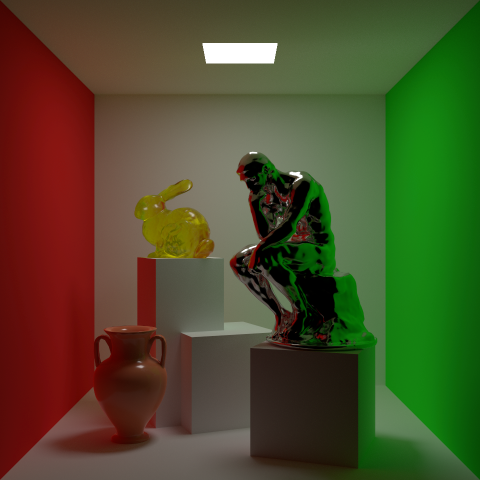
\includegraphics[width=\linewidth]{figures/py/tests/encodings/../quality_comparison/refpt_3min_thinker.png}
& 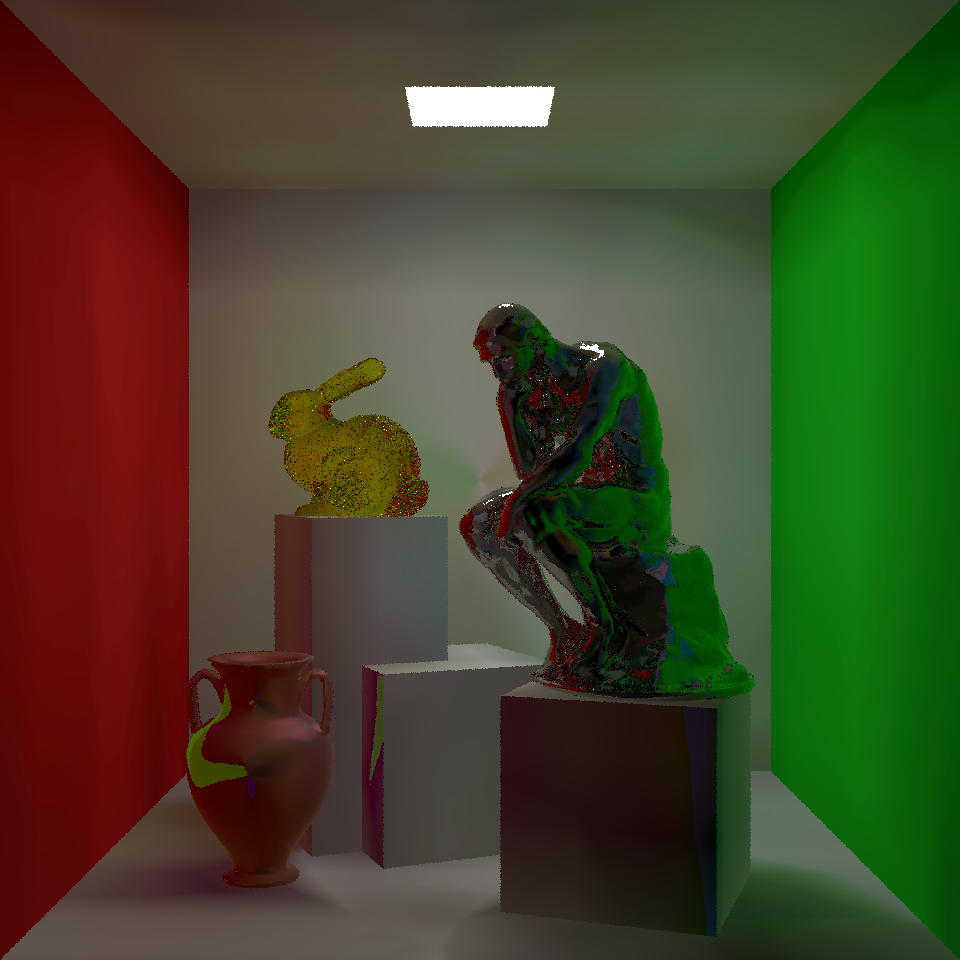
\includegraphics[width=\linewidth]{figures/py/tests/encodings/nrc+ptTWE_1spp.png}
& 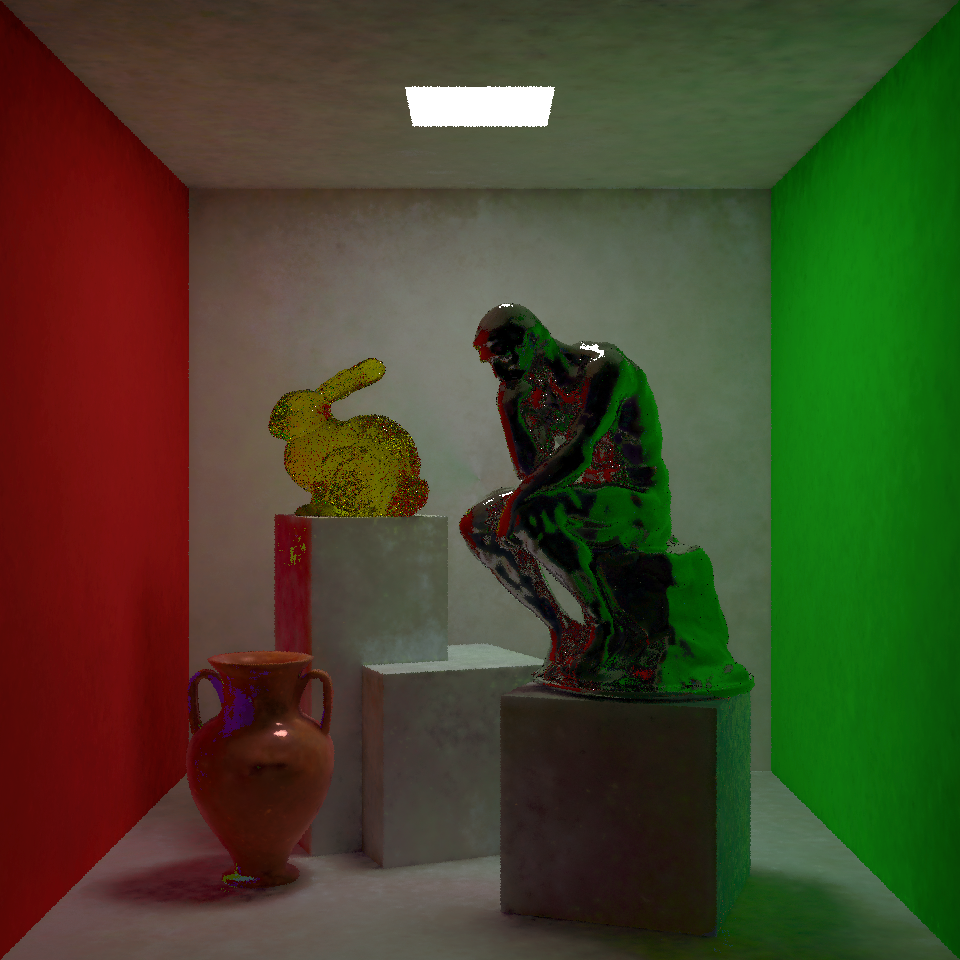
\includegraphics[width=\linewidth]{figures/py/tests/encodings/nrc+ptMHE_1spp.png}
\\
&& 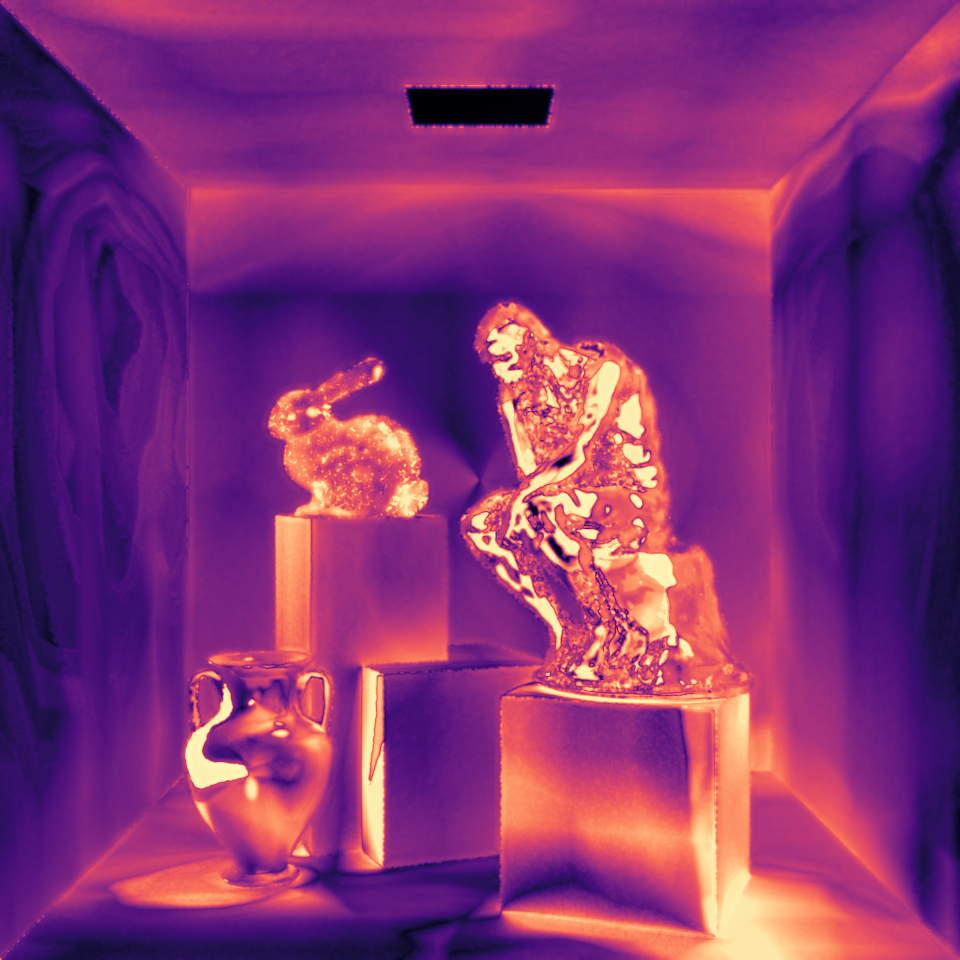
\includegraphics[width=\linewidth]{figures/py/tests/encodings/nrc+ptTWE_1spp_flip.png}
& 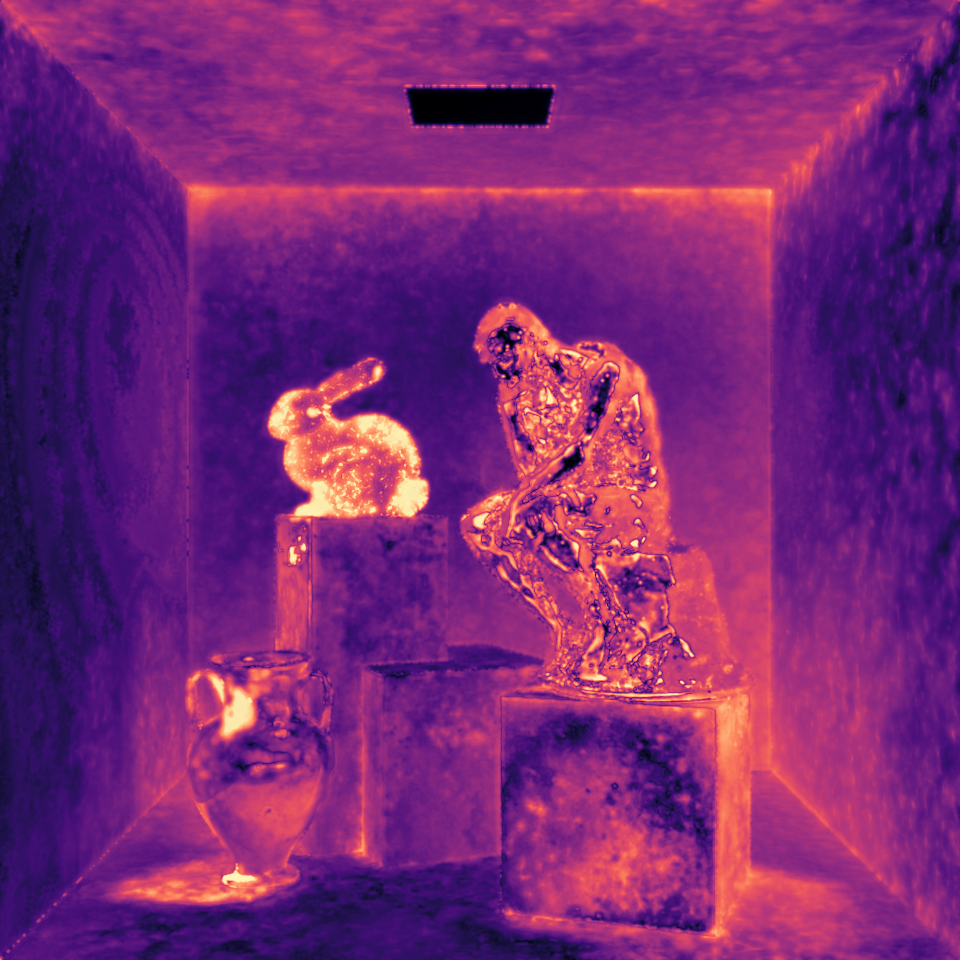
\includegraphics[width=\linewidth]{figures/py/tests/encodings/nrc+ptMHE_1spp_flip.png}
\\
&\FLIP/MSE: & \num{0.398}/\num{0.014}
 & \textbf{\num{0.359}}/\textbf{\num{0.014}}
\\
&$\mathrm{Bias}^2/\mathrm{Variance}$ & \num{1.70e-04}/\textbf{\num{1.48e-02}}
 & \textbf{\num{1.60e-04}}/\num{1.48e-02}
\\
\\
        \input{figures/py/tests/quality_comparison/Chess}\\
        \input{figures/py/tests/quality_comparison/Ajar}\\
        &2749spp (2m)
 & 1spp (116.80ms)
 & 1spp (\textbf{93.93ms})
 & 1spp (103.69ms)
\\
\rotatebox{90}{\textsc{Caustics}}\hspace{-1.5em}
&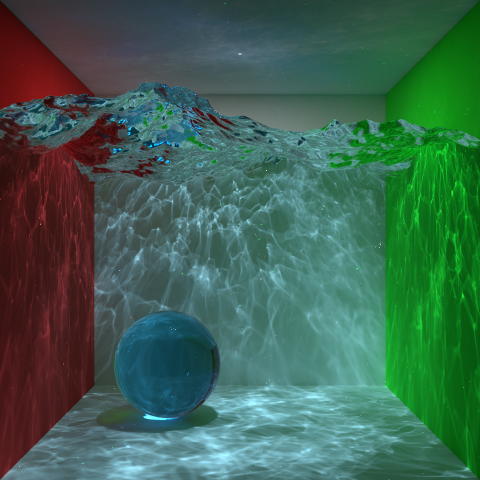
\includegraphics[width=\linewidth]{figures/py/tests/photon_optimization/ref_2min.png}
& 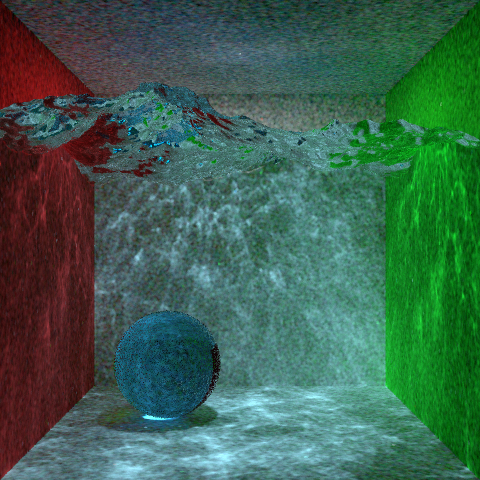
\includegraphics[width=\linewidth]{figures/py/tests/photon_optimization/SER_1spp.png}
& 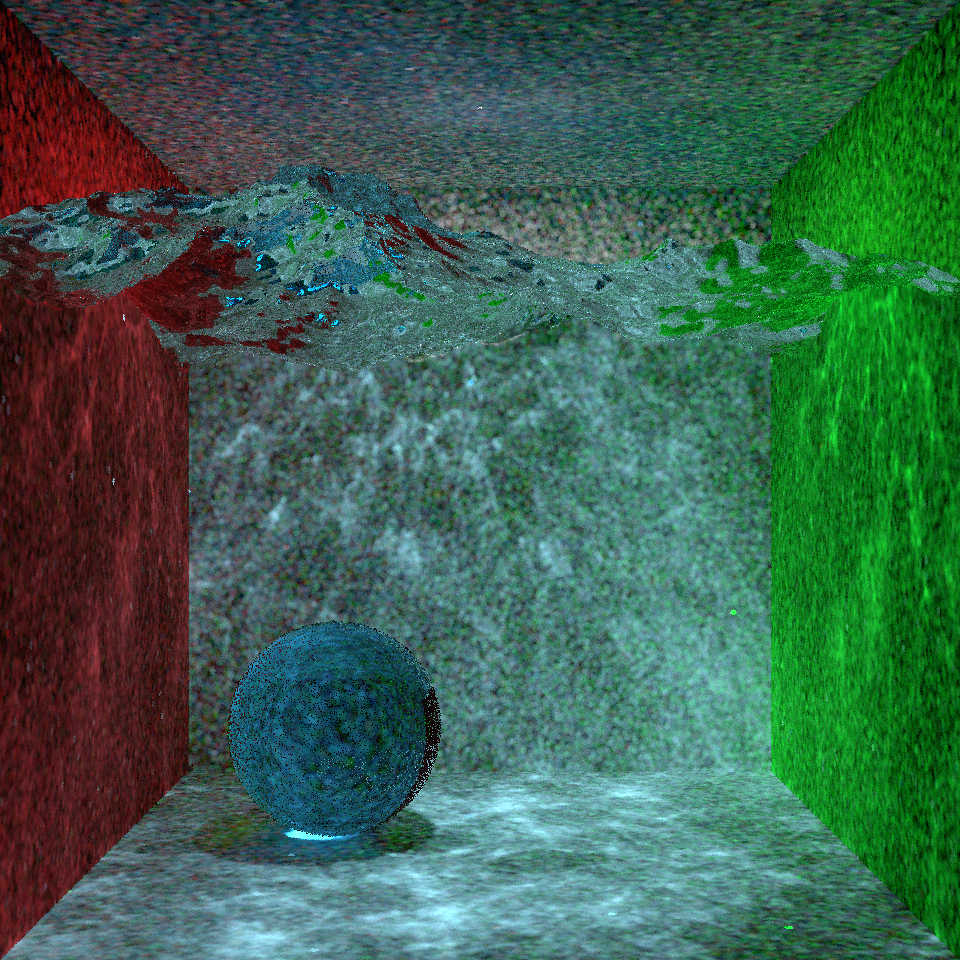
\includegraphics[width=\linewidth]{figures/py/tests/photon_optimization/SER+Reject70_1spp.png}
& 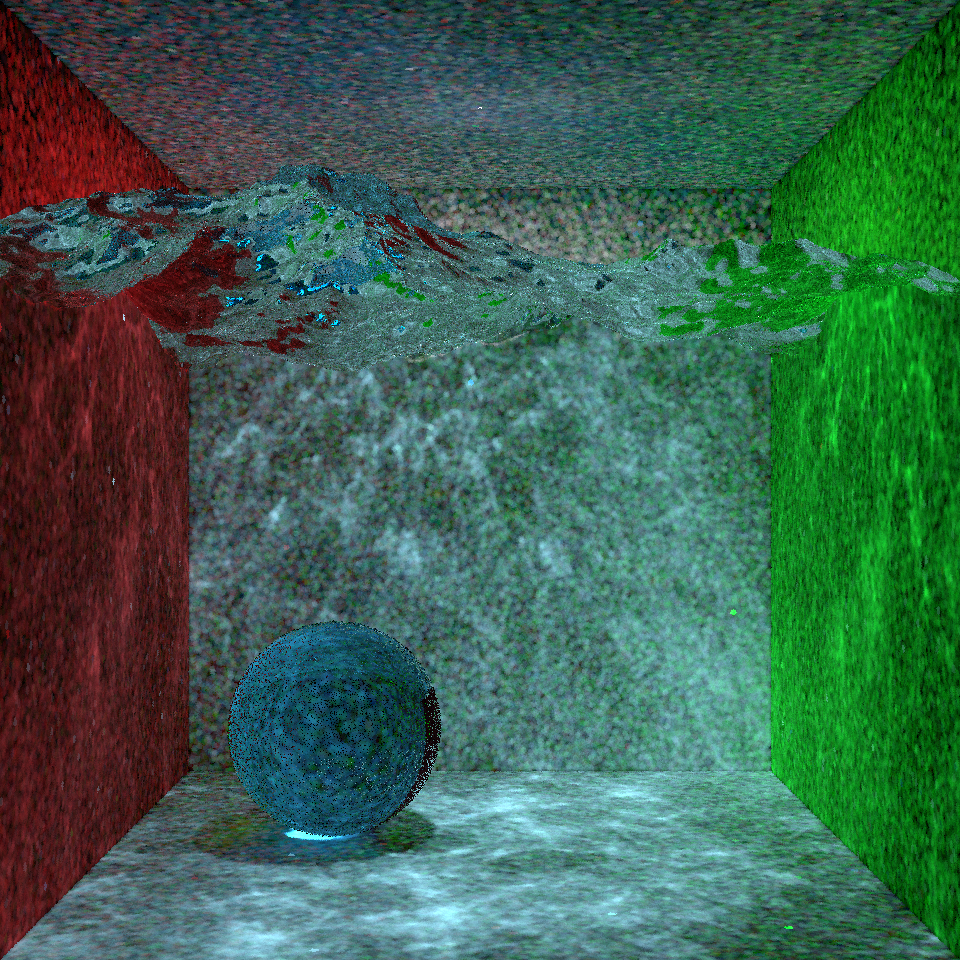
\includegraphics[width=\linewidth]{figures/py/tests/photon_optimization/SER+Reject70+RejectN_1spp.png}
\\
&& 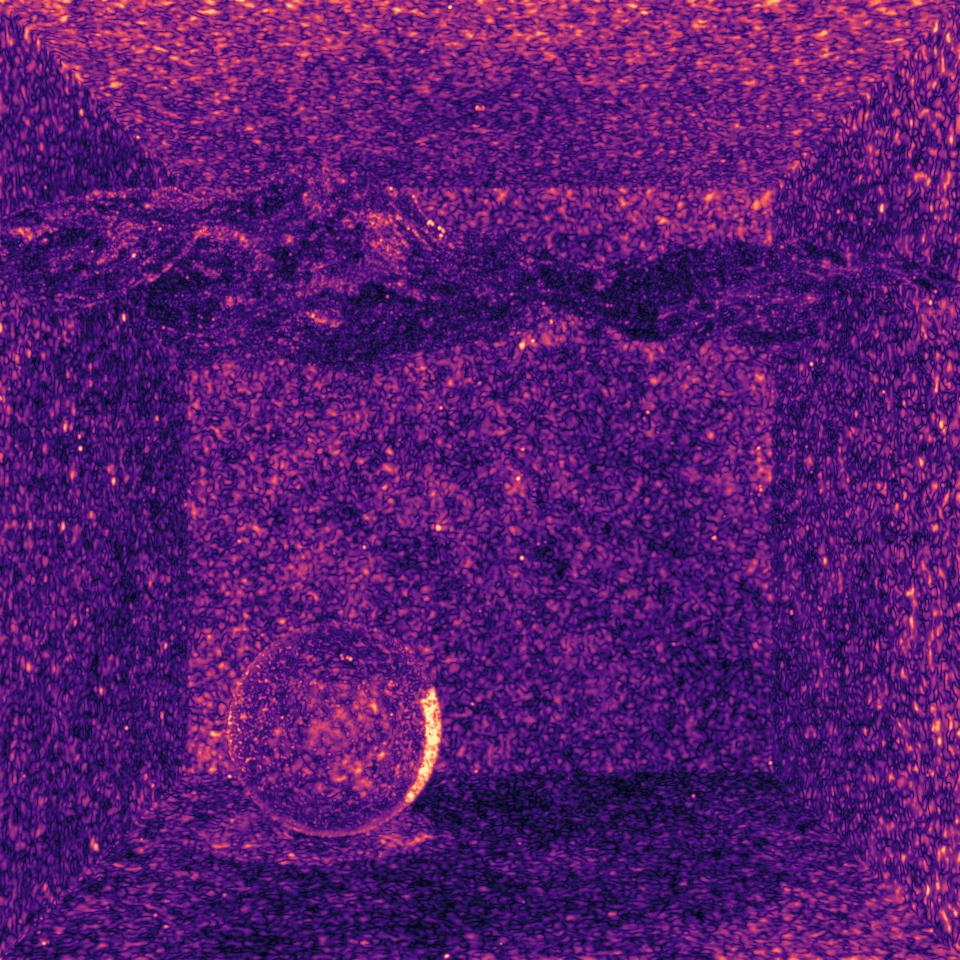
\includegraphics[width=\linewidth]{figures/py/tests/photon_optimization/SER_1spp_flip.png}
& 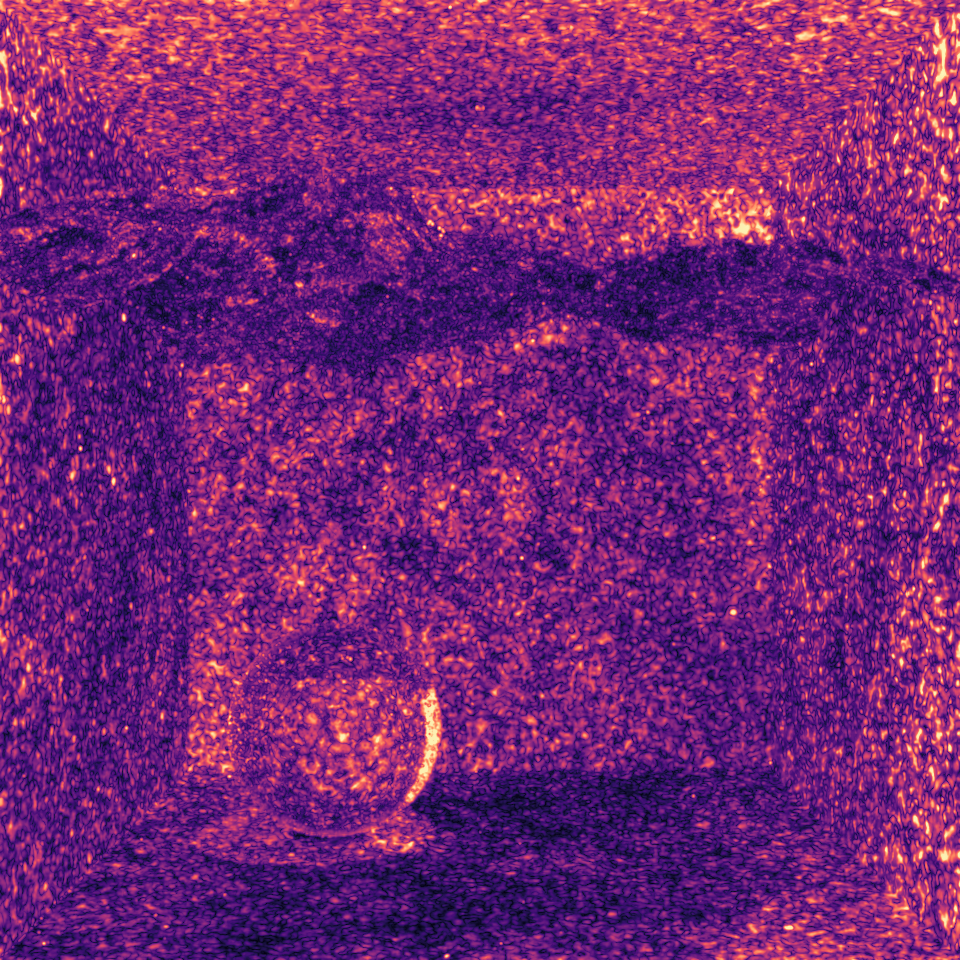
\includegraphics[width=\linewidth]{figures/py/tests/photon_optimization/SER+Reject70_1spp_flip.png}
& 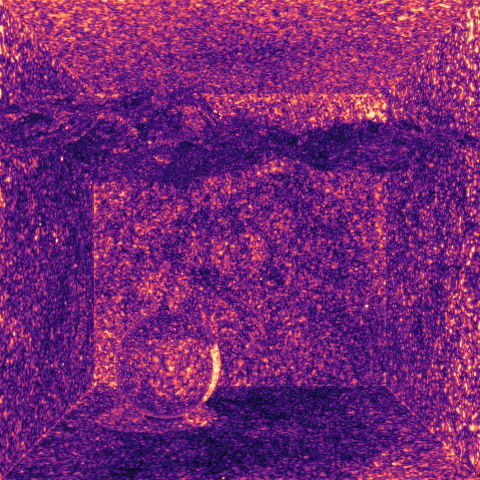
\includegraphics[width=\linewidth]{figures/py/tests/photon_optimization/SER+Reject70+RejectN_1spp_flip.png}
\\
&\FLIP/MSE: & \textbf{\num{0.272}}/\textbf{\num{973.693}}
 & \num{0.347}/\num{973.694}
 & \num{0.349}/\num{973.694}
\\
&$\mathrm{Bias}^2/\mathrm{Variance}$ & \textbf{\num{2.11e-07}}/\textbf{\num{4.24e+02}}
 & \num{2.32e-06}/\num{5.24e+02}
 & \num{1.57e-06}/\num{5.07e+02}
\\

    \end{tabularx}
    \caption{Comparison of the different radiance estimators from \autoref{chap:bidirectional_caching}. To isolate training quality, inference is terminated after the first diffuse vertex and is not combined with NEE.}
    \label{fig:quality_comparison}
\end{figure}

\section{Performance and Optimization}
\begin{figure}[ht]
    \centering
    \begin{subfigure}{0.5\textwidth}
        \centering
        \tiny
        \begin{tabularx}{\linewidth}{r*{4}{>{\centering\arraybackslash}X}}
            &Reference (SPPM) & SER & SER, 70\% & SER, 70\%, 30° \\
            &2749spp (2m)
 & 1spp (116.80ms)
 & 1spp (\textbf{93.93ms})
 & 1spp (103.69ms)
\\
\rotatebox{90}{\textsc{Caustics}}\hspace{-1.5em}
&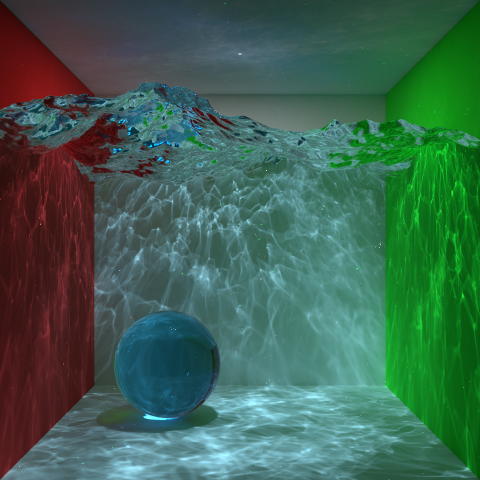
\includegraphics[width=\linewidth]{figures/py/tests/photon_optimization/ref_2min.png}
& 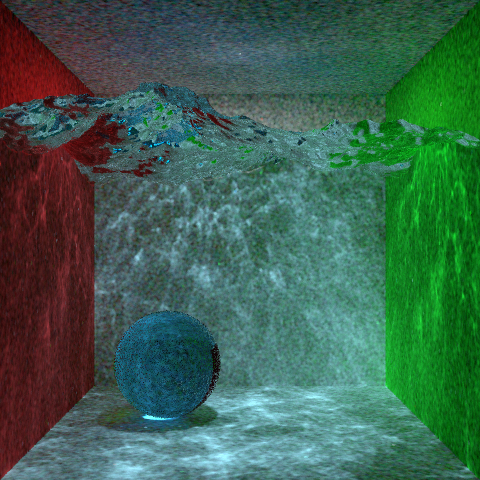
\includegraphics[width=\linewidth]{figures/py/tests/photon_optimization/SER_1spp.png}
& 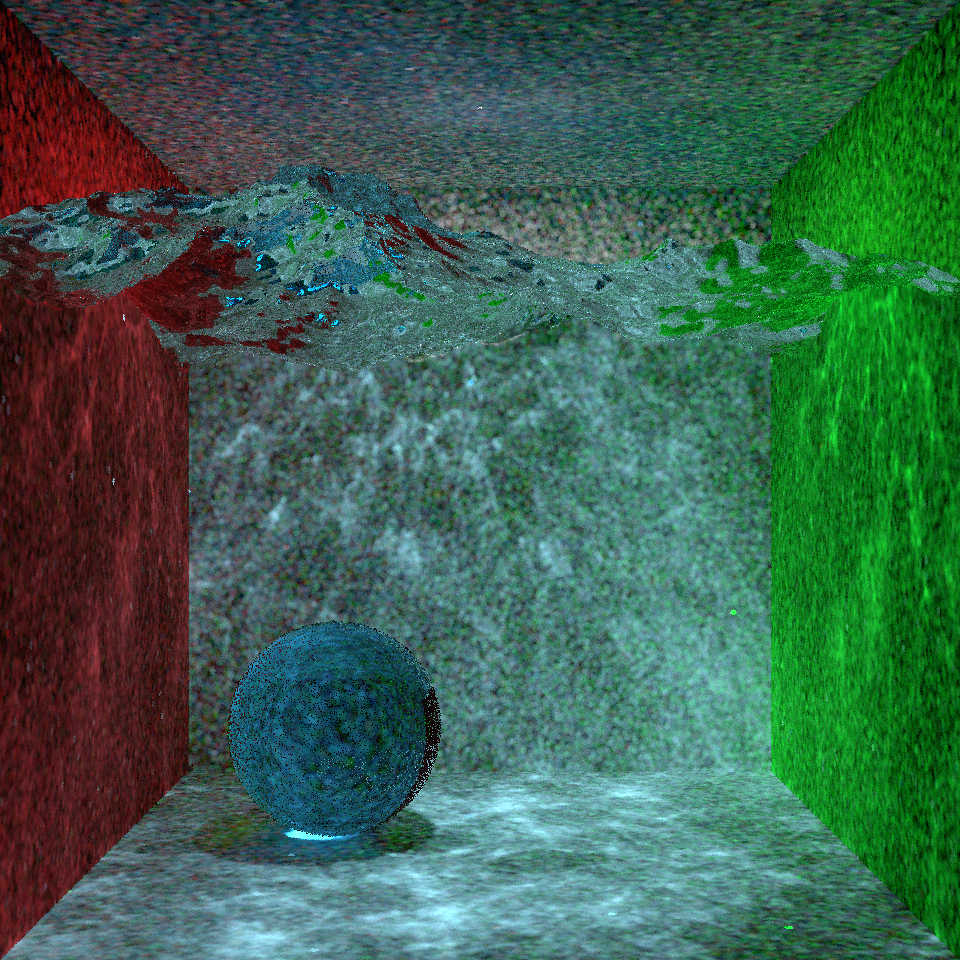
\includegraphics[width=\linewidth]{figures/py/tests/photon_optimization/SER+Reject70_1spp.png}
& 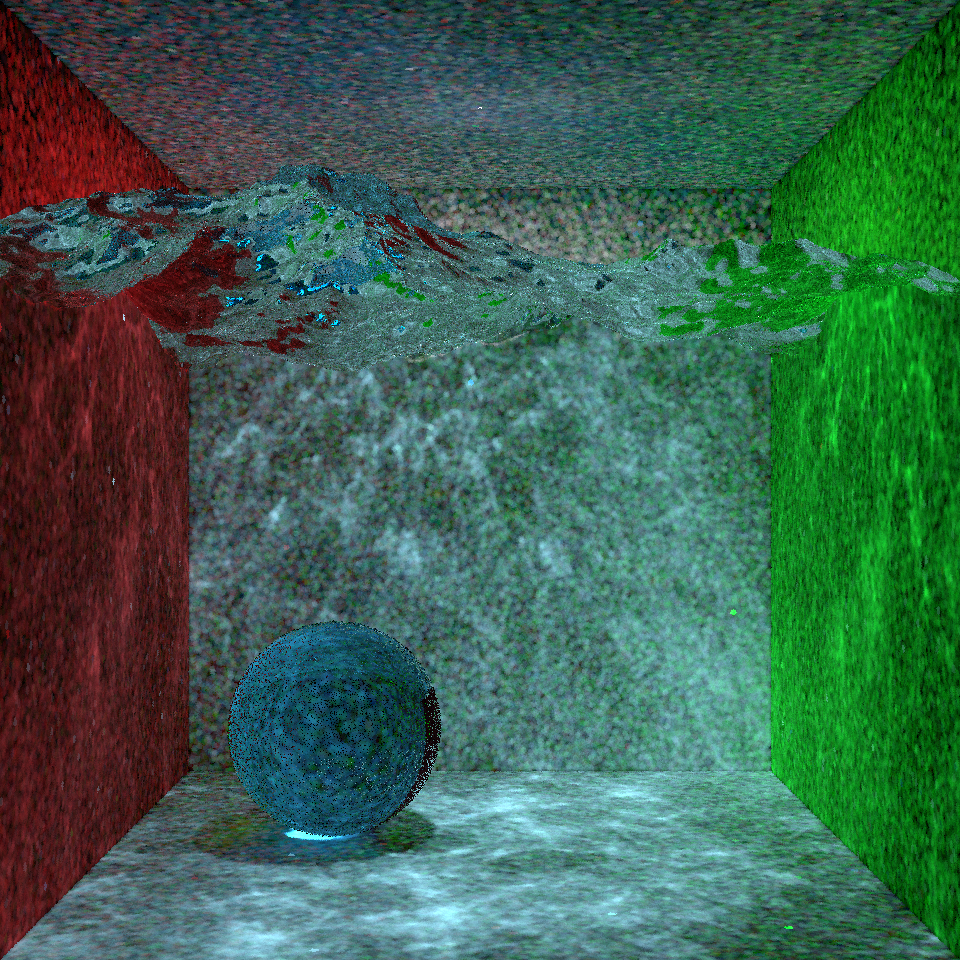
\includegraphics[width=\linewidth]{figures/py/tests/photon_optimization/SER+Reject70+RejectN_1spp.png}
\\
&& 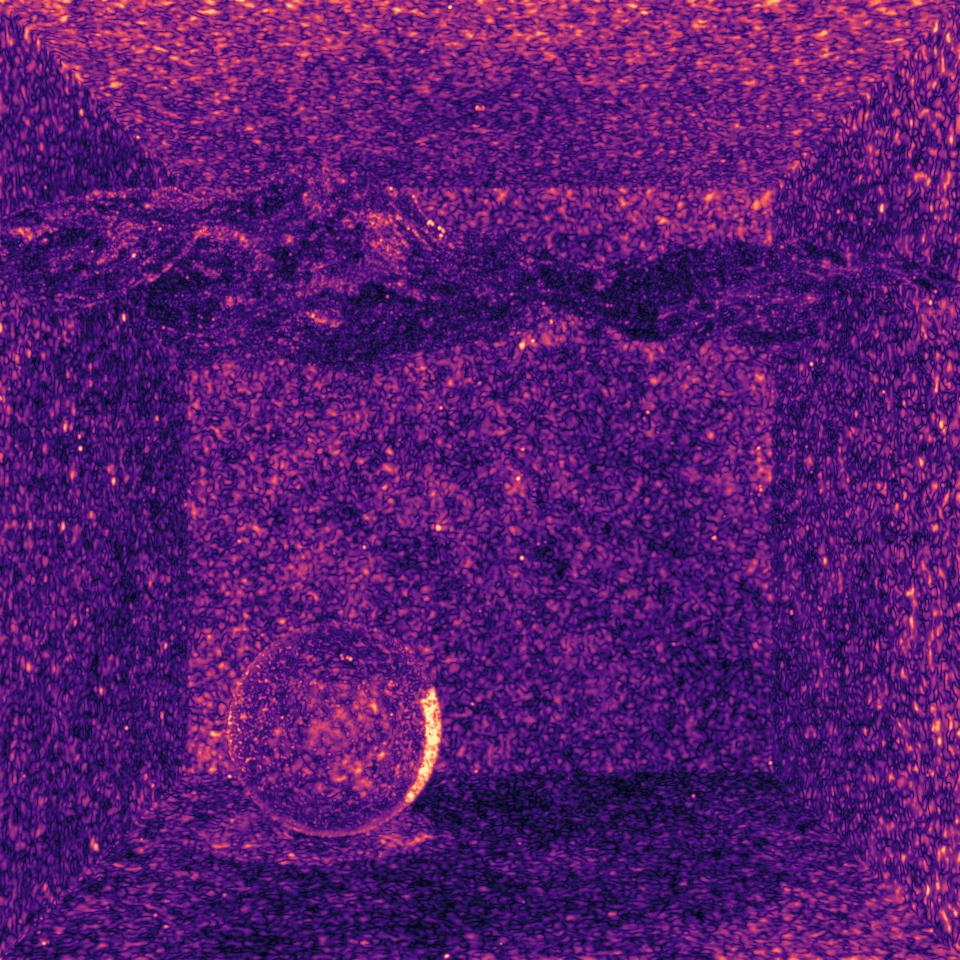
\includegraphics[width=\linewidth]{figures/py/tests/photon_optimization/SER_1spp_flip.png}
& 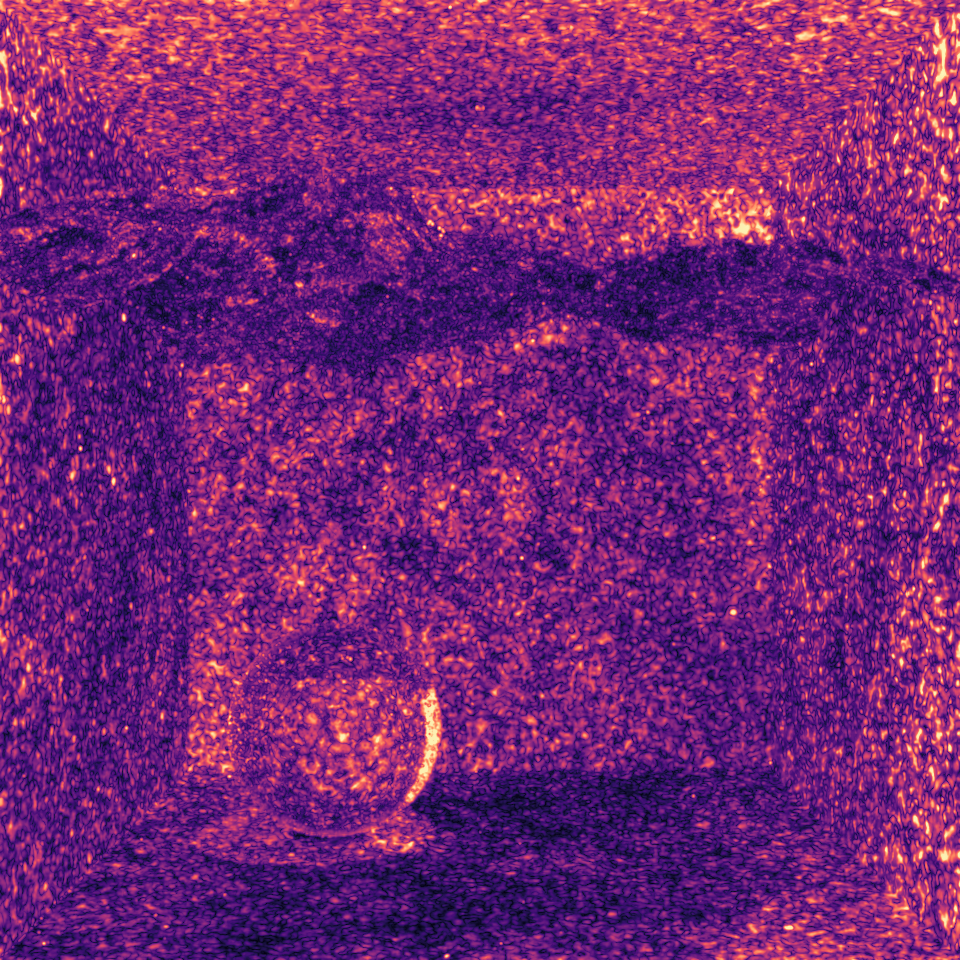
\includegraphics[width=\linewidth]{figures/py/tests/photon_optimization/SER+Reject70_1spp_flip.png}
& 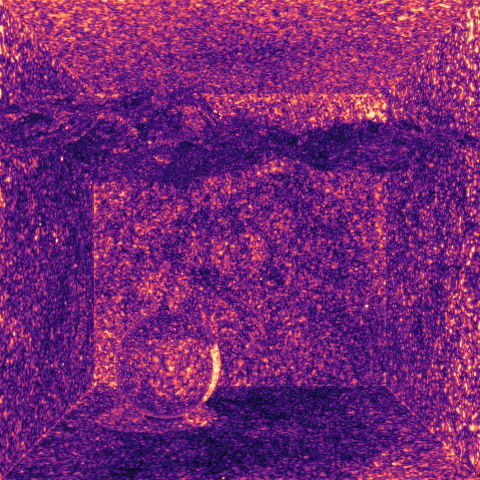
\includegraphics[width=\linewidth]{figures/py/tests/photon_optimization/SER+Reject70+RejectN_1spp_flip.png}
\\
&\FLIP/MSE: & \textbf{\num{0.272}}/\textbf{\num{973.693}}
 & \num{0.347}/\num{973.694}
 & \num{0.349}/\num{973.694}
\\
&$\mathrm{Bias}^2/\mathrm{Variance}$ & \textbf{\num{2.11e-07}}/\textbf{\num{4.24e+02}}
 & \num{2.32e-06}/\num{5.24e+02}
 & \num{1.57e-06}/\num{5.07e+02}
\\

        \end{tabularx}
    \end{subfigure}%
    \begin{subfigure}{0.5\textwidth}
        \centering
        \small
        \begin{tabular}{lll}
            \textbf{Technique} & \textbf{Frametime} & \textbf{Change} \\
            \midrule
            \textbf{Baseline} & \textbf{159.50ms} & \\
            IS only & 178.19ms & $+11.7\%$\\
            SER & 158.54ms & $-0.6\%$\\
            SER, 70\% & 124.46ms & $-22\%$\\
            SER, 70\%, 30$^{\circ}$ & 123.58ms & $-22.5\%$
        \end{tabular}
    \end{subfigure}
    \caption{Optimizations to Photon Mapping. \emph{IS only} directly accumulates in the Intersection Shader (IS) and skips the Any Hit Shader (AH). \emph{SER} uses Shader Execution Reordering between the Intersection and Any Hit shader to improve coherence. \emph{SER, 70\%} additionally rejects 70\% of the non-caustic photons in the Any Hit shader \parencite{kern2023}. \emph{SER, 70\%, 30$^{\circ}$} rejects photon hits whose surface normals deviate more than 30° from the surface normals at the query point \parencite{kern2023}. The most notable performance improvement comes from rejecting non-caustic photons, however, this notably increases error in non-caustic areas. Rejecting photons based on normal deviation has a small positive performance impact and decreases bias.}
\end{figure}

\begin{figure}
    \centering
    %% Creator: Matplotlib, PGF backend
%%
%% To include the figure in your LaTeX document, write
%%   \input{<filename>.pgf}
%%
%% Make sure the required packages are loaded in your preamble
%%   \usepackage{pgf}
%%
%% Also ensure that all the required font packages are loaded; for instance,
%% the lmodern package is sometimes necessary when using math font.
%%   \usepackage{lmodern}
%%
%% Figures using additional raster images can only be included by \input if
%% they are in the same directory as the main LaTeX file. For loading figures
%% from other directories you can use the `import` package
%%   \usepackage{import}
%%
%% and then include the figures with
%%   \import{<path to file>}{<filename>.pgf}
%%
%% Matplotlib used the following preamble
%%   \def\mathdefault#1{#1}
%%   \everymath=\expandafter{\the\everymath\displaystyle}
%%   \IfFileExists{scrextend.sty}{
%%     \usepackage[fontsize=10.000000pt]{scrextend}
%%   }{
%%     \renewcommand{\normalsize}{\fontsize{10.000000}{12.000000}\selectfont}
%%     \normalsize
%%   }
%%   
%%   \ifdefined\pdftexversion\else  % non-pdftex case.
%%     \usepackage{fontspec}
%%     \setmainfont{DejaVuSerif.ttf}[Path=\detokenize{/opt/homebrew/Cellar/python-matplotlib/3.10.5/libexec/lib/python3.13/site-packages/matplotlib/mpl-data/fonts/ttf/}]
%%     \setsansfont{DejaVuSans.ttf}[Path=\detokenize{/opt/homebrew/Cellar/python-matplotlib/3.10.5/libexec/lib/python3.13/site-packages/matplotlib/mpl-data/fonts/ttf/}]
%%     \setmonofont{DejaVuSansMono.ttf}[Path=\detokenize{/opt/homebrew/Cellar/python-matplotlib/3.10.5/libexec/lib/python3.13/site-packages/matplotlib/mpl-data/fonts/ttf/}]
%%   \fi
%%   \makeatletter\@ifpackageloaded{underscore}{}{\usepackage[strings]{underscore}}\makeatother
%%
\begingroup%
\makeatletter%
\begin{pgfpicture}%
\pgfpathrectangle{\pgfpointorigin}{\pgfqpoint{6.118122in}{3.116660in}}%
\pgfusepath{use as bounding box, clip}%
\begin{pgfscope}%
\pgfsetbuttcap%
\pgfsetmiterjoin%
\definecolor{currentfill}{rgb}{1.000000,1.000000,1.000000}%
\pgfsetfillcolor{currentfill}%
\pgfsetlinewidth{0.000000pt}%
\definecolor{currentstroke}{rgb}{1.000000,1.000000,1.000000}%
\pgfsetstrokecolor{currentstroke}%
\pgfsetdash{}{0pt}%
\pgfpathmoveto{\pgfqpoint{0.000000in}{0.000000in}}%
\pgfpathlineto{\pgfqpoint{6.118122in}{0.000000in}}%
\pgfpathlineto{\pgfqpoint{6.118122in}{3.116660in}}%
\pgfpathlineto{\pgfqpoint{0.000000in}{3.116660in}}%
\pgfpathlineto{\pgfqpoint{0.000000in}{0.000000in}}%
\pgfpathclose%
\pgfusepath{fill}%
\end{pgfscope}%
\begin{pgfscope}%
\pgfsetbuttcap%
\pgfsetmiterjoin%
\definecolor{currentfill}{rgb}{1.000000,1.000000,1.000000}%
\pgfsetfillcolor{currentfill}%
\pgfsetlinewidth{0.000000pt}%
\definecolor{currentstroke}{rgb}{0.000000,0.000000,0.000000}%
\pgfsetstrokecolor{currentstroke}%
\pgfsetstrokeopacity{0.000000}%
\pgfsetdash{}{0pt}%
\pgfpathmoveto{\pgfqpoint{2.060179in}{0.290505in}}%
\pgfpathlineto{\pgfqpoint{6.018122in}{0.290505in}}%
\pgfpathlineto{\pgfqpoint{6.018122in}{3.016660in}}%
\pgfpathlineto{\pgfqpoint{2.060179in}{3.016660in}}%
\pgfpathlineto{\pgfqpoint{2.060179in}{0.290505in}}%
\pgfpathclose%
\pgfusepath{fill}%
\end{pgfscope}%
\begin{pgfscope}%
\pgfpathrectangle{\pgfqpoint{2.060179in}{0.290505in}}{\pgfqpoint{3.957943in}{2.726155in}}%
\pgfusepath{clip}%
\pgfsetbuttcap%
\pgfsetmiterjoin%
\definecolor{currentfill}{rgb}{0.710588,0.710588,0.710588}%
\pgfsetfillcolor{currentfill}%
\pgfsetlinewidth{0.000000pt}%
\definecolor{currentstroke}{rgb}{0.000000,0.000000,0.000000}%
\pgfsetstrokecolor{currentstroke}%
\pgfsetstrokeopacity{0.000000}%
\pgfsetdash{}{0pt}%
\pgfpathmoveto{\pgfqpoint{2.240085in}{0.290505in}}%
\pgfpathlineto{\pgfqpoint{2.516864in}{0.290505in}}%
\pgfpathlineto{\pgfqpoint{2.516864in}{1.531982in}}%
\pgfpathlineto{\pgfqpoint{2.240085in}{1.531982in}}%
\pgfpathlineto{\pgfqpoint{2.240085in}{0.290505in}}%
\pgfpathclose%
\pgfusepath{fill}%
\end{pgfscope}%
\begin{pgfscope}%
\pgfpathrectangle{\pgfqpoint{2.060179in}{0.290505in}}{\pgfqpoint{3.957943in}{2.726155in}}%
\pgfusepath{clip}%
\pgfsetbuttcap%
\pgfsetmiterjoin%
\definecolor{currentfill}{rgb}{0.854902,0.439216,0.839216}%
\pgfsetfillcolor{currentfill}%
\pgfsetlinewidth{0.000000pt}%
\definecolor{currentstroke}{rgb}{0.000000,0.000000,0.000000}%
\pgfsetstrokecolor{currentstroke}%
\pgfsetstrokeopacity{0.000000}%
\pgfsetdash{}{0pt}%
\pgfpathmoveto{\pgfqpoint{2.240085in}{1.531982in}}%
\pgfpathlineto{\pgfqpoint{2.516864in}{1.531982in}}%
\pgfpathlineto{\pgfqpoint{2.516864in}{1.532932in}}%
\pgfpathlineto{\pgfqpoint{2.240085in}{1.532932in}}%
\pgfpathlineto{\pgfqpoint{2.240085in}{1.531982in}}%
\pgfpathclose%
\pgfusepath{fill}%
\end{pgfscope}%
\begin{pgfscope}%
\pgfpathrectangle{\pgfqpoint{2.060179in}{0.290505in}}{\pgfqpoint{3.957943in}{2.726155in}}%
\pgfusepath{clip}%
\pgfsetbuttcap%
\pgfsetmiterjoin%
\definecolor{currentfill}{rgb}{0.814118,0.883922,0.949804}%
\pgfsetfillcolor{currentfill}%
\pgfsetlinewidth{0.000000pt}%
\definecolor{currentstroke}{rgb}{0.000000,0.000000,0.000000}%
\pgfsetstrokecolor{currentstroke}%
\pgfsetstrokeopacity{0.000000}%
\pgfsetdash{}{0pt}%
\pgfpathmoveto{\pgfqpoint{2.793644in}{0.290505in}}%
\pgfpathlineto{\pgfqpoint{3.070423in}{0.290505in}}%
\pgfpathlineto{\pgfqpoint{3.070423in}{0.338908in}}%
\pgfpathlineto{\pgfqpoint{2.793644in}{0.338908in}}%
\pgfpathlineto{\pgfqpoint{2.793644in}{0.290505in}}%
\pgfpathclose%
\pgfusepath{fill}%
\end{pgfscope}%
\begin{pgfscope}%
\pgfpathrectangle{\pgfqpoint{2.060179in}{0.290505in}}{\pgfqpoint{3.957943in}{2.726155in}}%
\pgfusepath{clip}%
\pgfsetbuttcap%
\pgfsetmiterjoin%
\definecolor{currentfill}{rgb}{0.887059,0.887059,0.887059}%
\pgfsetfillcolor{currentfill}%
\pgfsetlinewidth{0.000000pt}%
\definecolor{currentstroke}{rgb}{0.000000,0.000000,0.000000}%
\pgfsetstrokecolor{currentstroke}%
\pgfsetstrokeopacity{0.000000}%
\pgfsetdash{}{0pt}%
\pgfpathmoveto{\pgfqpoint{2.793644in}{0.338908in}}%
\pgfpathlineto{\pgfqpoint{3.070423in}{0.338908in}}%
\pgfpathlineto{\pgfqpoint{3.070423in}{0.620419in}}%
\pgfpathlineto{\pgfqpoint{2.793644in}{0.620419in}}%
\pgfpathlineto{\pgfqpoint{2.793644in}{0.338908in}}%
\pgfpathclose%
\pgfusepath{fill}%
\end{pgfscope}%
\begin{pgfscope}%
\pgfpathrectangle{\pgfqpoint{2.060179in}{0.290505in}}{\pgfqpoint{3.957943in}{2.726155in}}%
\pgfusepath{clip}%
\pgfsetbuttcap%
\pgfsetmiterjoin%
\definecolor{currentfill}{rgb}{0.710588,0.710588,0.710588}%
\pgfsetfillcolor{currentfill}%
\pgfsetlinewidth{0.000000pt}%
\definecolor{currentstroke}{rgb}{0.000000,0.000000,0.000000}%
\pgfsetstrokecolor{currentstroke}%
\pgfsetstrokeopacity{0.000000}%
\pgfsetdash{}{0pt}%
\pgfpathmoveto{\pgfqpoint{2.793644in}{0.620419in}}%
\pgfpathlineto{\pgfqpoint{3.070423in}{0.620419in}}%
\pgfpathlineto{\pgfqpoint{3.070423in}{0.709444in}}%
\pgfpathlineto{\pgfqpoint{2.793644in}{0.709444in}}%
\pgfpathlineto{\pgfqpoint{2.793644in}{0.620419in}}%
\pgfpathclose%
\pgfusepath{fill}%
\end{pgfscope}%
\begin{pgfscope}%
\pgfpathrectangle{\pgfqpoint{2.060179in}{0.290505in}}{\pgfqpoint{3.957943in}{2.726155in}}%
\pgfusepath{clip}%
\pgfsetbuttcap%
\pgfsetmiterjoin%
\definecolor{currentfill}{rgb}{0.478431,0.478431,0.478431}%
\pgfsetfillcolor{currentfill}%
\pgfsetlinewidth{0.000000pt}%
\definecolor{currentstroke}{rgb}{0.000000,0.000000,0.000000}%
\pgfsetstrokecolor{currentstroke}%
\pgfsetstrokeopacity{0.000000}%
\pgfsetdash{}{0pt}%
\pgfpathmoveto{\pgfqpoint{2.793644in}{0.709444in}}%
\pgfpathlineto{\pgfqpoint{3.070423in}{0.709444in}}%
\pgfpathlineto{\pgfqpoint{3.070423in}{0.903746in}}%
\pgfpathlineto{\pgfqpoint{2.793644in}{0.903746in}}%
\pgfpathlineto{\pgfqpoint{2.793644in}{0.709444in}}%
\pgfpathclose%
\pgfusepath{fill}%
\end{pgfscope}%
\begin{pgfscope}%
\pgfpathrectangle{\pgfqpoint{2.060179in}{0.290505in}}{\pgfqpoint{3.957943in}{2.726155in}}%
\pgfusepath{clip}%
\pgfsetbuttcap%
\pgfsetmiterjoin%
\definecolor{currentfill}{rgb}{1.000000,0.752941,0.796078}%
\pgfsetfillcolor{currentfill}%
\pgfsetlinewidth{0.000000pt}%
\definecolor{currentstroke}{rgb}{0.000000,0.000000,0.000000}%
\pgfsetstrokecolor{currentstroke}%
\pgfsetstrokeopacity{0.000000}%
\pgfsetdash{}{0pt}%
\pgfpathmoveto{\pgfqpoint{2.793644in}{0.903746in}}%
\pgfpathlineto{\pgfqpoint{3.070423in}{0.903746in}}%
\pgfpathlineto{\pgfqpoint{3.070423in}{0.917474in}}%
\pgfpathlineto{\pgfqpoint{2.793644in}{0.917474in}}%
\pgfpathlineto{\pgfqpoint{2.793644in}{0.903746in}}%
\pgfpathclose%
\pgfusepath{fill}%
\end{pgfscope}%
\begin{pgfscope}%
\pgfpathrectangle{\pgfqpoint{2.060179in}{0.290505in}}{\pgfqpoint{3.957943in}{2.726155in}}%
\pgfusepath{clip}%
\pgfsetbuttcap%
\pgfsetmiterjoin%
\definecolor{currentfill}{rgb}{0.854902,0.439216,0.839216}%
\pgfsetfillcolor{currentfill}%
\pgfsetlinewidth{0.000000pt}%
\definecolor{currentstroke}{rgb}{0.000000,0.000000,0.000000}%
\pgfsetstrokecolor{currentstroke}%
\pgfsetstrokeopacity{0.000000}%
\pgfsetdash{}{0pt}%
\pgfpathmoveto{\pgfqpoint{2.793644in}{0.917474in}}%
\pgfpathlineto{\pgfqpoint{3.070423in}{0.917474in}}%
\pgfpathlineto{\pgfqpoint{3.070423in}{0.919898in}}%
\pgfpathlineto{\pgfqpoint{2.793644in}{0.919898in}}%
\pgfpathlineto{\pgfqpoint{2.793644in}{0.917474in}}%
\pgfpathclose%
\pgfusepath{fill}%
\end{pgfscope}%
\begin{pgfscope}%
\pgfpathrectangle{\pgfqpoint{2.060179in}{0.290505in}}{\pgfqpoint{3.957943in}{2.726155in}}%
\pgfusepath{clip}%
\pgfsetbuttcap%
\pgfsetmiterjoin%
\definecolor{currentfill}{rgb}{0.814118,0.883922,0.949804}%
\pgfsetfillcolor{currentfill}%
\pgfsetlinewidth{0.000000pt}%
\definecolor{currentstroke}{rgb}{0.000000,0.000000,0.000000}%
\pgfsetstrokecolor{currentstroke}%
\pgfsetstrokeopacity{0.000000}%
\pgfsetdash{}{0pt}%
\pgfpathmoveto{\pgfqpoint{3.347202in}{0.290505in}}%
\pgfpathlineto{\pgfqpoint{3.623981in}{0.290505in}}%
\pgfpathlineto{\pgfqpoint{3.623981in}{0.355218in}}%
\pgfpathlineto{\pgfqpoint{3.347202in}{0.355218in}}%
\pgfpathlineto{\pgfqpoint{3.347202in}{0.290505in}}%
\pgfpathclose%
\pgfusepath{fill}%
\end{pgfscope}%
\begin{pgfscope}%
\pgfpathrectangle{\pgfqpoint{2.060179in}{0.290505in}}{\pgfqpoint{3.957943in}{2.726155in}}%
\pgfusepath{clip}%
\pgfsetbuttcap%
\pgfsetmiterjoin%
\definecolor{currentfill}{rgb}{0.827451,0.932549,0.803137}%
\pgfsetfillcolor{currentfill}%
\pgfsetlinewidth{0.000000pt}%
\definecolor{currentstroke}{rgb}{0.000000,0.000000,0.000000}%
\pgfsetstrokecolor{currentstroke}%
\pgfsetstrokeopacity{0.000000}%
\pgfsetdash{}{0pt}%
\pgfpathmoveto{\pgfqpoint{3.347202in}{0.355218in}}%
\pgfpathlineto{\pgfqpoint{3.623981in}{0.355218in}}%
\pgfpathlineto{\pgfqpoint{3.623981in}{0.385085in}}%
\pgfpathlineto{\pgfqpoint{3.347202in}{0.385085in}}%
\pgfpathlineto{\pgfqpoint{3.347202in}{0.355218in}}%
\pgfpathclose%
\pgfusepath{fill}%
\end{pgfscope}%
\begin{pgfscope}%
\pgfpathrectangle{\pgfqpoint{2.060179in}{0.290505in}}{\pgfqpoint{3.957943in}{2.726155in}}%
\pgfusepath{clip}%
\pgfsetbuttcap%
\pgfsetmiterjoin%
\definecolor{currentfill}{rgb}{0.451765,0.767090,0.461207}%
\pgfsetfillcolor{currentfill}%
\pgfsetlinewidth{0.000000pt}%
\definecolor{currentstroke}{rgb}{0.000000,0.000000,0.000000}%
\pgfsetstrokecolor{currentstroke}%
\pgfsetstrokeopacity{0.000000}%
\pgfsetdash{}{0pt}%
\pgfpathmoveto{\pgfqpoint{3.347202in}{0.385085in}}%
\pgfpathlineto{\pgfqpoint{3.623981in}{0.385085in}}%
\pgfpathlineto{\pgfqpoint{3.623981in}{0.393893in}}%
\pgfpathlineto{\pgfqpoint{3.347202in}{0.393893in}}%
\pgfpathlineto{\pgfqpoint{3.347202in}{0.385085in}}%
\pgfpathclose%
\pgfusepath{fill}%
\end{pgfscope}%
\begin{pgfscope}%
\pgfpathrectangle{\pgfqpoint{2.060179in}{0.290505in}}{\pgfqpoint{3.957943in}{2.726155in}}%
\pgfusepath{clip}%
\pgfsetbuttcap%
\pgfsetmiterjoin%
\definecolor{currentfill}{rgb}{0.887059,0.887059,0.887059}%
\pgfsetfillcolor{currentfill}%
\pgfsetlinewidth{0.000000pt}%
\definecolor{currentstroke}{rgb}{0.000000,0.000000,0.000000}%
\pgfsetstrokecolor{currentstroke}%
\pgfsetstrokeopacity{0.000000}%
\pgfsetdash{}{0pt}%
\pgfpathmoveto{\pgfqpoint{3.347202in}{0.393893in}}%
\pgfpathlineto{\pgfqpoint{3.623981in}{0.393893in}}%
\pgfpathlineto{\pgfqpoint{3.623981in}{0.706840in}}%
\pgfpathlineto{\pgfqpoint{3.347202in}{0.706840in}}%
\pgfpathlineto{\pgfqpoint{3.347202in}{0.393893in}}%
\pgfpathclose%
\pgfusepath{fill}%
\end{pgfscope}%
\begin{pgfscope}%
\pgfpathrectangle{\pgfqpoint{2.060179in}{0.290505in}}{\pgfqpoint{3.957943in}{2.726155in}}%
\pgfusepath{clip}%
\pgfsetbuttcap%
\pgfsetmiterjoin%
\definecolor{currentfill}{rgb}{0.710588,0.710588,0.710588}%
\pgfsetfillcolor{currentfill}%
\pgfsetlinewidth{0.000000pt}%
\definecolor{currentstroke}{rgb}{0.000000,0.000000,0.000000}%
\pgfsetstrokecolor{currentstroke}%
\pgfsetstrokeopacity{0.000000}%
\pgfsetdash{}{0pt}%
\pgfpathmoveto{\pgfqpoint{3.347202in}{0.706840in}}%
\pgfpathlineto{\pgfqpoint{3.623981in}{0.706840in}}%
\pgfpathlineto{\pgfqpoint{3.623981in}{0.824404in}}%
\pgfpathlineto{\pgfqpoint{3.347202in}{0.824404in}}%
\pgfpathlineto{\pgfqpoint{3.347202in}{0.706840in}}%
\pgfpathclose%
\pgfusepath{fill}%
\end{pgfscope}%
\begin{pgfscope}%
\pgfpathrectangle{\pgfqpoint{2.060179in}{0.290505in}}{\pgfqpoint{3.957943in}{2.726155in}}%
\pgfusepath{clip}%
\pgfsetbuttcap%
\pgfsetmiterjoin%
\definecolor{currentfill}{rgb}{0.478431,0.478431,0.478431}%
\pgfsetfillcolor{currentfill}%
\pgfsetlinewidth{0.000000pt}%
\definecolor{currentstroke}{rgb}{0.000000,0.000000,0.000000}%
\pgfsetstrokecolor{currentstroke}%
\pgfsetstrokeopacity{0.000000}%
\pgfsetdash{}{0pt}%
\pgfpathmoveto{\pgfqpoint{3.347202in}{0.824404in}}%
\pgfpathlineto{\pgfqpoint{3.623981in}{0.824404in}}%
\pgfpathlineto{\pgfqpoint{3.623981in}{1.039657in}}%
\pgfpathlineto{\pgfqpoint{3.347202in}{1.039657in}}%
\pgfpathlineto{\pgfqpoint{3.347202in}{0.824404in}}%
\pgfpathclose%
\pgfusepath{fill}%
\end{pgfscope}%
\begin{pgfscope}%
\pgfpathrectangle{\pgfqpoint{2.060179in}{0.290505in}}{\pgfqpoint{3.957943in}{2.726155in}}%
\pgfusepath{clip}%
\pgfsetbuttcap%
\pgfsetmiterjoin%
\definecolor{currentfill}{rgb}{1.000000,0.752941,0.796078}%
\pgfsetfillcolor{currentfill}%
\pgfsetlinewidth{0.000000pt}%
\definecolor{currentstroke}{rgb}{0.000000,0.000000,0.000000}%
\pgfsetstrokecolor{currentstroke}%
\pgfsetstrokeopacity{0.000000}%
\pgfsetdash{}{0pt}%
\pgfpathmoveto{\pgfqpoint{3.347202in}{1.039657in}}%
\pgfpathlineto{\pgfqpoint{3.623981in}{1.039657in}}%
\pgfpathlineto{\pgfqpoint{3.623981in}{1.053399in}}%
\pgfpathlineto{\pgfqpoint{3.347202in}{1.053399in}}%
\pgfpathlineto{\pgfqpoint{3.347202in}{1.039657in}}%
\pgfpathclose%
\pgfusepath{fill}%
\end{pgfscope}%
\begin{pgfscope}%
\pgfpathrectangle{\pgfqpoint{2.060179in}{0.290505in}}{\pgfqpoint{3.957943in}{2.726155in}}%
\pgfusepath{clip}%
\pgfsetbuttcap%
\pgfsetmiterjoin%
\definecolor{currentfill}{rgb}{0.854902,0.439216,0.839216}%
\pgfsetfillcolor{currentfill}%
\pgfsetlinewidth{0.000000pt}%
\definecolor{currentstroke}{rgb}{0.000000,0.000000,0.000000}%
\pgfsetstrokecolor{currentstroke}%
\pgfsetstrokeopacity{0.000000}%
\pgfsetdash{}{0pt}%
\pgfpathmoveto{\pgfqpoint{3.347202in}{1.053399in}}%
\pgfpathlineto{\pgfqpoint{3.623981in}{1.053399in}}%
\pgfpathlineto{\pgfqpoint{3.623981in}{1.067114in}}%
\pgfpathlineto{\pgfqpoint{3.347202in}{1.067114in}}%
\pgfpathlineto{\pgfqpoint{3.347202in}{1.053399in}}%
\pgfpathclose%
\pgfusepath{fill}%
\end{pgfscope}%
\begin{pgfscope}%
\pgfpathrectangle{\pgfqpoint{2.060179in}{0.290505in}}{\pgfqpoint{3.957943in}{2.726155in}}%
\pgfusepath{clip}%
\pgfsetbuttcap%
\pgfsetmiterjoin%
\definecolor{currentfill}{rgb}{0.579608,0.770196,0.873725}%
\pgfsetfillcolor{currentfill}%
\pgfsetlinewidth{0.000000pt}%
\definecolor{currentstroke}{rgb}{0.000000,0.000000,0.000000}%
\pgfsetstrokecolor{currentstroke}%
\pgfsetstrokeopacity{0.000000}%
\pgfsetdash{}{0pt}%
\pgfpathmoveto{\pgfqpoint{3.900761in}{0.290505in}}%
\pgfpathlineto{\pgfqpoint{4.177540in}{0.290505in}}%
\pgfpathlineto{\pgfqpoint{4.177540in}{0.337256in}}%
\pgfpathlineto{\pgfqpoint{3.900761in}{0.337256in}}%
\pgfpathlineto{\pgfqpoint{3.900761in}{0.290505in}}%
\pgfpathclose%
\pgfusepath{fill}%
\end{pgfscope}%
\begin{pgfscope}%
\pgfpathrectangle{\pgfqpoint{2.060179in}{0.290505in}}{\pgfqpoint{3.957943in}{2.726155in}}%
\pgfusepath{clip}%
\pgfsetbuttcap%
\pgfsetmiterjoin%
\definecolor{currentfill}{rgb}{0.887059,0.887059,0.887059}%
\pgfsetfillcolor{currentfill}%
\pgfsetlinewidth{0.000000pt}%
\definecolor{currentstroke}{rgb}{0.000000,0.000000,0.000000}%
\pgfsetstrokecolor{currentstroke}%
\pgfsetstrokeopacity{0.000000}%
\pgfsetdash{}{0pt}%
\pgfpathmoveto{\pgfqpoint{3.900761in}{0.337256in}}%
\pgfpathlineto{\pgfqpoint{4.177540in}{0.337256in}}%
\pgfpathlineto{\pgfqpoint{4.177540in}{0.613994in}}%
\pgfpathlineto{\pgfqpoint{3.900761in}{0.613994in}}%
\pgfpathlineto{\pgfqpoint{3.900761in}{0.337256in}}%
\pgfpathclose%
\pgfusepath{fill}%
\end{pgfscope}%
\begin{pgfscope}%
\pgfpathrectangle{\pgfqpoint{2.060179in}{0.290505in}}{\pgfqpoint{3.957943in}{2.726155in}}%
\pgfusepath{clip}%
\pgfsetbuttcap%
\pgfsetmiterjoin%
\definecolor{currentfill}{rgb}{0.710588,0.710588,0.710588}%
\pgfsetfillcolor{currentfill}%
\pgfsetlinewidth{0.000000pt}%
\definecolor{currentstroke}{rgb}{0.000000,0.000000,0.000000}%
\pgfsetstrokecolor{currentstroke}%
\pgfsetstrokeopacity{0.000000}%
\pgfsetdash{}{0pt}%
\pgfpathmoveto{\pgfqpoint{3.900761in}{0.613994in}}%
\pgfpathlineto{\pgfqpoint{4.177540in}{0.613994in}}%
\pgfpathlineto{\pgfqpoint{4.177540in}{0.702965in}}%
\pgfpathlineto{\pgfqpoint{3.900761in}{0.702965in}}%
\pgfpathlineto{\pgfqpoint{3.900761in}{0.613994in}}%
\pgfpathclose%
\pgfusepath{fill}%
\end{pgfscope}%
\begin{pgfscope}%
\pgfpathrectangle{\pgfqpoint{2.060179in}{0.290505in}}{\pgfqpoint{3.957943in}{2.726155in}}%
\pgfusepath{clip}%
\pgfsetbuttcap%
\pgfsetmiterjoin%
\definecolor{currentfill}{rgb}{0.478431,0.478431,0.478431}%
\pgfsetfillcolor{currentfill}%
\pgfsetlinewidth{0.000000pt}%
\definecolor{currentstroke}{rgb}{0.000000,0.000000,0.000000}%
\pgfsetstrokecolor{currentstroke}%
\pgfsetstrokeopacity{0.000000}%
\pgfsetdash{}{0pt}%
\pgfpathmoveto{\pgfqpoint{3.900761in}{0.702965in}}%
\pgfpathlineto{\pgfqpoint{4.177540in}{0.702965in}}%
\pgfpathlineto{\pgfqpoint{4.177540in}{0.897140in}}%
\pgfpathlineto{\pgfqpoint{3.900761in}{0.897140in}}%
\pgfpathlineto{\pgfqpoint{3.900761in}{0.702965in}}%
\pgfpathclose%
\pgfusepath{fill}%
\end{pgfscope}%
\begin{pgfscope}%
\pgfpathrectangle{\pgfqpoint{2.060179in}{0.290505in}}{\pgfqpoint{3.957943in}{2.726155in}}%
\pgfusepath{clip}%
\pgfsetbuttcap%
\pgfsetmiterjoin%
\definecolor{currentfill}{rgb}{1.000000,0.752941,0.796078}%
\pgfsetfillcolor{currentfill}%
\pgfsetlinewidth{0.000000pt}%
\definecolor{currentstroke}{rgb}{0.000000,0.000000,0.000000}%
\pgfsetstrokecolor{currentstroke}%
\pgfsetstrokeopacity{0.000000}%
\pgfsetdash{}{0pt}%
\pgfpathmoveto{\pgfqpoint{3.900761in}{0.897140in}}%
\pgfpathlineto{\pgfqpoint{4.177540in}{0.897140in}}%
\pgfpathlineto{\pgfqpoint{4.177540in}{0.910873in}}%
\pgfpathlineto{\pgfqpoint{3.900761in}{0.910873in}}%
\pgfpathlineto{\pgfqpoint{3.900761in}{0.897140in}}%
\pgfpathclose%
\pgfusepath{fill}%
\end{pgfscope}%
\begin{pgfscope}%
\pgfpathrectangle{\pgfqpoint{2.060179in}{0.290505in}}{\pgfqpoint{3.957943in}{2.726155in}}%
\pgfusepath{clip}%
\pgfsetbuttcap%
\pgfsetmiterjoin%
\definecolor{currentfill}{rgb}{0.854902,0.439216,0.839216}%
\pgfsetfillcolor{currentfill}%
\pgfsetlinewidth{0.000000pt}%
\definecolor{currentstroke}{rgb}{0.000000,0.000000,0.000000}%
\pgfsetstrokecolor{currentstroke}%
\pgfsetstrokeopacity{0.000000}%
\pgfsetdash{}{0pt}%
\pgfpathmoveto{\pgfqpoint{3.900761in}{0.910873in}}%
\pgfpathlineto{\pgfqpoint{4.177540in}{0.910873in}}%
\pgfpathlineto{\pgfqpoint{4.177540in}{0.913381in}}%
\pgfpathlineto{\pgfqpoint{3.900761in}{0.913381in}}%
\pgfpathlineto{\pgfqpoint{3.900761in}{0.910873in}}%
\pgfpathclose%
\pgfusepath{fill}%
\end{pgfscope}%
\begin{pgfscope}%
\pgfpathrectangle{\pgfqpoint{2.060179in}{0.290505in}}{\pgfqpoint{3.957943in}{2.726155in}}%
\pgfusepath{clip}%
\pgfsetbuttcap%
\pgfsetmiterjoin%
\definecolor{currentfill}{rgb}{0.579608,0.770196,0.873725}%
\pgfsetfillcolor{currentfill}%
\pgfsetlinewidth{0.000000pt}%
\definecolor{currentstroke}{rgb}{0.000000,0.000000,0.000000}%
\pgfsetstrokecolor{currentstroke}%
\pgfsetstrokeopacity{0.000000}%
\pgfsetdash{}{0pt}%
\pgfpathmoveto{\pgfqpoint{4.454319in}{0.290505in}}%
\pgfpathlineto{\pgfqpoint{4.731098in}{0.290505in}}%
\pgfpathlineto{\pgfqpoint{4.731098in}{0.487897in}}%
\pgfpathlineto{\pgfqpoint{4.454319in}{0.487897in}}%
\pgfpathlineto{\pgfqpoint{4.454319in}{0.290505in}}%
\pgfpathclose%
\pgfusepath{fill}%
\end{pgfscope}%
\begin{pgfscope}%
\pgfpathrectangle{\pgfqpoint{2.060179in}{0.290505in}}{\pgfqpoint{3.957943in}{2.726155in}}%
\pgfusepath{clip}%
\pgfsetbuttcap%
\pgfsetmiterjoin%
\definecolor{currentfill}{rgb}{0.887059,0.887059,0.887059}%
\pgfsetfillcolor{currentfill}%
\pgfsetlinewidth{0.000000pt}%
\definecolor{currentstroke}{rgb}{0.000000,0.000000,0.000000}%
\pgfsetstrokecolor{currentstroke}%
\pgfsetstrokeopacity{0.000000}%
\pgfsetdash{}{0pt}%
\pgfpathmoveto{\pgfqpoint{4.454319in}{0.487897in}}%
\pgfpathlineto{\pgfqpoint{4.731098in}{0.487897in}}%
\pgfpathlineto{\pgfqpoint{4.731098in}{0.768069in}}%
\pgfpathlineto{\pgfqpoint{4.454319in}{0.768069in}}%
\pgfpathlineto{\pgfqpoint{4.454319in}{0.487897in}}%
\pgfpathclose%
\pgfusepath{fill}%
\end{pgfscope}%
\begin{pgfscope}%
\pgfpathrectangle{\pgfqpoint{2.060179in}{0.290505in}}{\pgfqpoint{3.957943in}{2.726155in}}%
\pgfusepath{clip}%
\pgfsetbuttcap%
\pgfsetmiterjoin%
\definecolor{currentfill}{rgb}{0.710588,0.710588,0.710588}%
\pgfsetfillcolor{currentfill}%
\pgfsetlinewidth{0.000000pt}%
\definecolor{currentstroke}{rgb}{0.000000,0.000000,0.000000}%
\pgfsetstrokecolor{currentstroke}%
\pgfsetstrokeopacity{0.000000}%
\pgfsetdash{}{0pt}%
\pgfpathmoveto{\pgfqpoint{4.454319in}{0.768069in}}%
\pgfpathlineto{\pgfqpoint{4.731098in}{0.768069in}}%
\pgfpathlineto{\pgfqpoint{4.731098in}{0.857112in}}%
\pgfpathlineto{\pgfqpoint{4.454319in}{0.857112in}}%
\pgfpathlineto{\pgfqpoint{4.454319in}{0.768069in}}%
\pgfpathclose%
\pgfusepath{fill}%
\end{pgfscope}%
\begin{pgfscope}%
\pgfpathrectangle{\pgfqpoint{2.060179in}{0.290505in}}{\pgfqpoint{3.957943in}{2.726155in}}%
\pgfusepath{clip}%
\pgfsetbuttcap%
\pgfsetmiterjoin%
\definecolor{currentfill}{rgb}{0.478431,0.478431,0.478431}%
\pgfsetfillcolor{currentfill}%
\pgfsetlinewidth{0.000000pt}%
\definecolor{currentstroke}{rgb}{0.000000,0.000000,0.000000}%
\pgfsetstrokecolor{currentstroke}%
\pgfsetstrokeopacity{0.000000}%
\pgfsetdash{}{0pt}%
\pgfpathmoveto{\pgfqpoint{4.454319in}{0.857112in}}%
\pgfpathlineto{\pgfqpoint{4.731098in}{0.857112in}}%
\pgfpathlineto{\pgfqpoint{4.731098in}{1.051332in}}%
\pgfpathlineto{\pgfqpoint{4.454319in}{1.051332in}}%
\pgfpathlineto{\pgfqpoint{4.454319in}{0.857112in}}%
\pgfpathclose%
\pgfusepath{fill}%
\end{pgfscope}%
\begin{pgfscope}%
\pgfpathrectangle{\pgfqpoint{2.060179in}{0.290505in}}{\pgfqpoint{3.957943in}{2.726155in}}%
\pgfusepath{clip}%
\pgfsetbuttcap%
\pgfsetmiterjoin%
\definecolor{currentfill}{rgb}{1.000000,0.752941,0.796078}%
\pgfsetfillcolor{currentfill}%
\pgfsetlinewidth{0.000000pt}%
\definecolor{currentstroke}{rgb}{0.000000,0.000000,0.000000}%
\pgfsetstrokecolor{currentstroke}%
\pgfsetstrokeopacity{0.000000}%
\pgfsetdash{}{0pt}%
\pgfpathmoveto{\pgfqpoint{4.454319in}{1.051332in}}%
\pgfpathlineto{\pgfqpoint{4.731098in}{1.051332in}}%
\pgfpathlineto{\pgfqpoint{4.731098in}{1.065057in}}%
\pgfpathlineto{\pgfqpoint{4.454319in}{1.065057in}}%
\pgfpathlineto{\pgfqpoint{4.454319in}{1.051332in}}%
\pgfpathclose%
\pgfusepath{fill}%
\end{pgfscope}%
\begin{pgfscope}%
\pgfpathrectangle{\pgfqpoint{2.060179in}{0.290505in}}{\pgfqpoint{3.957943in}{2.726155in}}%
\pgfusepath{clip}%
\pgfsetbuttcap%
\pgfsetmiterjoin%
\definecolor{currentfill}{rgb}{0.854902,0.439216,0.839216}%
\pgfsetfillcolor{currentfill}%
\pgfsetlinewidth{0.000000pt}%
\definecolor{currentstroke}{rgb}{0.000000,0.000000,0.000000}%
\pgfsetstrokecolor{currentstroke}%
\pgfsetstrokeopacity{0.000000}%
\pgfsetdash{}{0pt}%
\pgfpathmoveto{\pgfqpoint{4.454319in}{1.065057in}}%
\pgfpathlineto{\pgfqpoint{4.731098in}{1.065057in}}%
\pgfpathlineto{\pgfqpoint{4.731098in}{1.067490in}}%
\pgfpathlineto{\pgfqpoint{4.454319in}{1.067490in}}%
\pgfpathlineto{\pgfqpoint{4.454319in}{1.065057in}}%
\pgfpathclose%
\pgfusepath{fill}%
\end{pgfscope}%
\begin{pgfscope}%
\pgfpathrectangle{\pgfqpoint{2.060179in}{0.290505in}}{\pgfqpoint{3.957943in}{2.726155in}}%
\pgfusepath{clip}%
\pgfsetbuttcap%
\pgfsetmiterjoin%
\definecolor{currentfill}{rgb}{0.993725,0.850196,0.704314}%
\pgfsetfillcolor{currentfill}%
\pgfsetlinewidth{0.000000pt}%
\definecolor{currentstroke}{rgb}{0.000000,0.000000,0.000000}%
\pgfsetstrokecolor{currentstroke}%
\pgfsetstrokeopacity{0.000000}%
\pgfsetdash{}{0pt}%
\pgfpathmoveto{\pgfqpoint{5.007877in}{0.290505in}}%
\pgfpathlineto{\pgfqpoint{5.284657in}{0.290505in}}%
\pgfpathlineto{\pgfqpoint{5.284657in}{0.297129in}}%
\pgfpathlineto{\pgfqpoint{5.007877in}{0.297129in}}%
\pgfpathlineto{\pgfqpoint{5.007877in}{0.290505in}}%
\pgfpathclose%
\pgfusepath{fill}%
\end{pgfscope}%
\begin{pgfscope}%
\pgfpathrectangle{\pgfqpoint{2.060179in}{0.290505in}}{\pgfqpoint{3.957943in}{2.726155in}}%
\pgfusepath{clip}%
\pgfsetbuttcap%
\pgfsetmiterjoin%
\definecolor{currentfill}{rgb}{0.992157,0.710065,0.464437}%
\pgfsetfillcolor{currentfill}%
\pgfsetlinewidth{0.000000pt}%
\definecolor{currentstroke}{rgb}{0.000000,0.000000,0.000000}%
\pgfsetstrokecolor{currentstroke}%
\pgfsetstrokeopacity{0.000000}%
\pgfsetdash{}{0pt}%
\pgfpathmoveto{\pgfqpoint{5.007877in}{0.297129in}}%
\pgfpathlineto{\pgfqpoint{5.284657in}{0.297129in}}%
\pgfpathlineto{\pgfqpoint{5.284657in}{0.339028in}}%
\pgfpathlineto{\pgfqpoint{5.007877in}{0.339028in}}%
\pgfpathlineto{\pgfqpoint{5.007877in}{0.297129in}}%
\pgfpathclose%
\pgfusepath{fill}%
\end{pgfscope}%
\begin{pgfscope}%
\pgfpathrectangle{\pgfqpoint{2.060179in}{0.290505in}}{\pgfqpoint{3.957943in}{2.726155in}}%
\pgfusepath{clip}%
\pgfsetbuttcap%
\pgfsetmiterjoin%
\definecolor{currentfill}{rgb}{0.991419,0.550727,0.232772}%
\pgfsetfillcolor{currentfill}%
\pgfsetlinewidth{0.000000pt}%
\definecolor{currentstroke}{rgb}{0.000000,0.000000,0.000000}%
\pgfsetstrokecolor{currentstroke}%
\pgfsetstrokeopacity{0.000000}%
\pgfsetdash{}{0pt}%
\pgfpathmoveto{\pgfqpoint{5.007877in}{0.339028in}}%
\pgfpathlineto{\pgfqpoint{5.284657in}{0.339028in}}%
\pgfpathlineto{\pgfqpoint{5.284657in}{0.601046in}}%
\pgfpathlineto{\pgfqpoint{5.007877in}{0.601046in}}%
\pgfpathlineto{\pgfqpoint{5.007877in}{0.339028in}}%
\pgfpathclose%
\pgfusepath{fill}%
\end{pgfscope}%
\begin{pgfscope}%
\pgfpathrectangle{\pgfqpoint{2.060179in}{0.290505in}}{\pgfqpoint{3.957943in}{2.726155in}}%
\pgfusepath{clip}%
\pgfsetbuttcap%
\pgfsetmiterjoin%
\definecolor{currentfill}{rgb}{0.925536,0.384867,0.059839}%
\pgfsetfillcolor{currentfill}%
\pgfsetlinewidth{0.000000pt}%
\definecolor{currentstroke}{rgb}{0.000000,0.000000,0.000000}%
\pgfsetstrokecolor{currentstroke}%
\pgfsetstrokeopacity{0.000000}%
\pgfsetdash{}{0pt}%
\pgfpathmoveto{\pgfqpoint{5.007877in}{0.601046in}}%
\pgfpathlineto{\pgfqpoint{5.284657in}{0.601046in}}%
\pgfpathlineto{\pgfqpoint{5.284657in}{0.609503in}}%
\pgfpathlineto{\pgfqpoint{5.007877in}{0.609503in}}%
\pgfpathlineto{\pgfqpoint{5.007877in}{0.601046in}}%
\pgfpathclose%
\pgfusepath{fill}%
\end{pgfscope}%
\begin{pgfscope}%
\pgfpathrectangle{\pgfqpoint{2.060179in}{0.290505in}}{\pgfqpoint{3.957943in}{2.726155in}}%
\pgfusepath{clip}%
\pgfsetbuttcap%
\pgfsetmiterjoin%
\definecolor{currentfill}{rgb}{0.887059,0.887059,0.887059}%
\pgfsetfillcolor{currentfill}%
\pgfsetlinewidth{0.000000pt}%
\definecolor{currentstroke}{rgb}{0.000000,0.000000,0.000000}%
\pgfsetstrokecolor{currentstroke}%
\pgfsetstrokeopacity{0.000000}%
\pgfsetdash{}{0pt}%
\pgfpathmoveto{\pgfqpoint{5.007877in}{0.609503in}}%
\pgfpathlineto{\pgfqpoint{5.284657in}{0.609503in}}%
\pgfpathlineto{\pgfqpoint{5.284657in}{0.908102in}}%
\pgfpathlineto{\pgfqpoint{5.007877in}{0.908102in}}%
\pgfpathlineto{\pgfqpoint{5.007877in}{0.609503in}}%
\pgfpathclose%
\pgfusepath{fill}%
\end{pgfscope}%
\begin{pgfscope}%
\pgfpathrectangle{\pgfqpoint{2.060179in}{0.290505in}}{\pgfqpoint{3.957943in}{2.726155in}}%
\pgfusepath{clip}%
\pgfsetbuttcap%
\pgfsetmiterjoin%
\definecolor{currentfill}{rgb}{0.710588,0.710588,0.710588}%
\pgfsetfillcolor{currentfill}%
\pgfsetlinewidth{0.000000pt}%
\definecolor{currentstroke}{rgb}{0.000000,0.000000,0.000000}%
\pgfsetstrokecolor{currentstroke}%
\pgfsetstrokeopacity{0.000000}%
\pgfsetdash{}{0pt}%
\pgfpathmoveto{\pgfqpoint{5.007877in}{0.908102in}}%
\pgfpathlineto{\pgfqpoint{5.284657in}{0.908102in}}%
\pgfpathlineto{\pgfqpoint{5.284657in}{0.997261in}}%
\pgfpathlineto{\pgfqpoint{5.007877in}{0.997261in}}%
\pgfpathlineto{\pgfqpoint{5.007877in}{0.908102in}}%
\pgfpathclose%
\pgfusepath{fill}%
\end{pgfscope}%
\begin{pgfscope}%
\pgfpathrectangle{\pgfqpoint{2.060179in}{0.290505in}}{\pgfqpoint{3.957943in}{2.726155in}}%
\pgfusepath{clip}%
\pgfsetbuttcap%
\pgfsetmiterjoin%
\definecolor{currentfill}{rgb}{0.478431,0.478431,0.478431}%
\pgfsetfillcolor{currentfill}%
\pgfsetlinewidth{0.000000pt}%
\definecolor{currentstroke}{rgb}{0.000000,0.000000,0.000000}%
\pgfsetstrokecolor{currentstroke}%
\pgfsetstrokeopacity{0.000000}%
\pgfsetdash{}{0pt}%
\pgfpathmoveto{\pgfqpoint{5.007877in}{0.997261in}}%
\pgfpathlineto{\pgfqpoint{5.284657in}{0.997261in}}%
\pgfpathlineto{\pgfqpoint{5.284657in}{1.191919in}}%
\pgfpathlineto{\pgfqpoint{5.007877in}{1.191919in}}%
\pgfpathlineto{\pgfqpoint{5.007877in}{0.997261in}}%
\pgfpathclose%
\pgfusepath{fill}%
\end{pgfscope}%
\begin{pgfscope}%
\pgfpathrectangle{\pgfqpoint{2.060179in}{0.290505in}}{\pgfqpoint{3.957943in}{2.726155in}}%
\pgfusepath{clip}%
\pgfsetbuttcap%
\pgfsetmiterjoin%
\definecolor{currentfill}{rgb}{1.000000,0.752941,0.796078}%
\pgfsetfillcolor{currentfill}%
\pgfsetlinewidth{0.000000pt}%
\definecolor{currentstroke}{rgb}{0.000000,0.000000,0.000000}%
\pgfsetstrokecolor{currentstroke}%
\pgfsetstrokeopacity{0.000000}%
\pgfsetdash{}{0pt}%
\pgfpathmoveto{\pgfqpoint{5.007877in}{1.191919in}}%
\pgfpathlineto{\pgfqpoint{5.284657in}{1.191919in}}%
\pgfpathlineto{\pgfqpoint{5.284657in}{1.205650in}}%
\pgfpathlineto{\pgfqpoint{5.007877in}{1.205650in}}%
\pgfpathlineto{\pgfqpoint{5.007877in}{1.191919in}}%
\pgfpathclose%
\pgfusepath{fill}%
\end{pgfscope}%
\begin{pgfscope}%
\pgfpathrectangle{\pgfqpoint{2.060179in}{0.290505in}}{\pgfqpoint{3.957943in}{2.726155in}}%
\pgfusepath{clip}%
\pgfsetbuttcap%
\pgfsetmiterjoin%
\definecolor{currentfill}{rgb}{0.854902,0.439216,0.839216}%
\pgfsetfillcolor{currentfill}%
\pgfsetlinewidth{0.000000pt}%
\definecolor{currentstroke}{rgb}{0.000000,0.000000,0.000000}%
\pgfsetstrokecolor{currentstroke}%
\pgfsetstrokeopacity{0.000000}%
\pgfsetdash{}{0pt}%
\pgfpathmoveto{\pgfqpoint{5.007877in}{1.205650in}}%
\pgfpathlineto{\pgfqpoint{5.284657in}{1.205650in}}%
\pgfpathlineto{\pgfqpoint{5.284657in}{1.211475in}}%
\pgfpathlineto{\pgfqpoint{5.007877in}{1.211475in}}%
\pgfpathlineto{\pgfqpoint{5.007877in}{1.205650in}}%
\pgfpathclose%
\pgfusepath{fill}%
\end{pgfscope}%
\begin{pgfscope}%
\pgfpathrectangle{\pgfqpoint{2.060179in}{0.290505in}}{\pgfqpoint{3.957943in}{2.726155in}}%
\pgfusepath{clip}%
\pgfsetbuttcap%
\pgfsetmiterjoin%
\definecolor{currentfill}{rgb}{0.993725,0.850196,0.704314}%
\pgfsetfillcolor{currentfill}%
\pgfsetlinewidth{0.000000pt}%
\definecolor{currentstroke}{rgb}{0.000000,0.000000,0.000000}%
\pgfsetstrokecolor{currentstroke}%
\pgfsetstrokeopacity{0.000000}%
\pgfsetdash{}{0pt}%
\pgfpathmoveto{\pgfqpoint{5.561436in}{0.290505in}}%
\pgfpathlineto{\pgfqpoint{5.838215in}{0.290505in}}%
\pgfpathlineto{\pgfqpoint{5.838215in}{0.439441in}}%
\pgfpathlineto{\pgfqpoint{5.561436in}{0.439441in}}%
\pgfpathlineto{\pgfqpoint{5.561436in}{0.290505in}}%
\pgfpathclose%
\pgfusepath{fill}%
\end{pgfscope}%
\begin{pgfscope}%
\pgfpathrectangle{\pgfqpoint{2.060179in}{0.290505in}}{\pgfqpoint{3.957943in}{2.726155in}}%
\pgfusepath{clip}%
\pgfsetbuttcap%
\pgfsetmiterjoin%
\definecolor{currentfill}{rgb}{0.992157,0.710065,0.464437}%
\pgfsetfillcolor{currentfill}%
\pgfsetlinewidth{0.000000pt}%
\definecolor{currentstroke}{rgb}{0.000000,0.000000,0.000000}%
\pgfsetstrokecolor{currentstroke}%
\pgfsetstrokeopacity{0.000000}%
\pgfsetdash{}{0pt}%
\pgfpathmoveto{\pgfqpoint{5.561436in}{0.439441in}}%
\pgfpathlineto{\pgfqpoint{5.838215in}{0.439441in}}%
\pgfpathlineto{\pgfqpoint{5.838215in}{0.681824in}}%
\pgfpathlineto{\pgfqpoint{5.561436in}{0.681824in}}%
\pgfpathlineto{\pgfqpoint{5.561436in}{0.439441in}}%
\pgfpathclose%
\pgfusepath{fill}%
\end{pgfscope}%
\begin{pgfscope}%
\pgfpathrectangle{\pgfqpoint{2.060179in}{0.290505in}}{\pgfqpoint{3.957943in}{2.726155in}}%
\pgfusepath{clip}%
\pgfsetbuttcap%
\pgfsetmiterjoin%
\definecolor{currentfill}{rgb}{0.991419,0.550727,0.232772}%
\pgfsetfillcolor{currentfill}%
\pgfsetlinewidth{0.000000pt}%
\definecolor{currentstroke}{rgb}{0.000000,0.000000,0.000000}%
\pgfsetstrokecolor{currentstroke}%
\pgfsetstrokeopacity{0.000000}%
\pgfsetdash{}{0pt}%
\pgfpathmoveto{\pgfqpoint{5.561436in}{0.681824in}}%
\pgfpathlineto{\pgfqpoint{5.838215in}{0.681824in}}%
\pgfpathlineto{\pgfqpoint{5.838215in}{2.439834in}}%
\pgfpathlineto{\pgfqpoint{5.561436in}{2.439834in}}%
\pgfpathlineto{\pgfqpoint{5.561436in}{0.681824in}}%
\pgfpathclose%
\pgfusepath{fill}%
\end{pgfscope}%
\begin{pgfscope}%
\pgfpathrectangle{\pgfqpoint{2.060179in}{0.290505in}}{\pgfqpoint{3.957943in}{2.726155in}}%
\pgfusepath{clip}%
\pgfsetbuttcap%
\pgfsetmiterjoin%
\definecolor{currentfill}{rgb}{1.000000,0.752941,0.796078}%
\pgfsetfillcolor{currentfill}%
\pgfsetlinewidth{0.000000pt}%
\definecolor{currentstroke}{rgb}{0.000000,0.000000,0.000000}%
\pgfsetstrokecolor{currentstroke}%
\pgfsetstrokeopacity{0.000000}%
\pgfsetdash{}{0pt}%
\pgfpathmoveto{\pgfqpoint{5.561436in}{2.439834in}}%
\pgfpathlineto{\pgfqpoint{5.838215in}{2.439834in}}%
\pgfpathlineto{\pgfqpoint{5.838215in}{2.460186in}}%
\pgfpathlineto{\pgfqpoint{5.561436in}{2.460186in}}%
\pgfpathlineto{\pgfqpoint{5.561436in}{2.439834in}}%
\pgfpathclose%
\pgfusepath{fill}%
\end{pgfscope}%
\begin{pgfscope}%
\pgfpathrectangle{\pgfqpoint{2.060179in}{0.290505in}}{\pgfqpoint{3.957943in}{2.726155in}}%
\pgfusepath{clip}%
\pgfsetbuttcap%
\pgfsetmiterjoin%
\definecolor{currentfill}{rgb}{0.854902,0.439216,0.839216}%
\pgfsetfillcolor{currentfill}%
\pgfsetlinewidth{0.000000pt}%
\definecolor{currentstroke}{rgb}{0.000000,0.000000,0.000000}%
\pgfsetstrokecolor{currentstroke}%
\pgfsetstrokeopacity{0.000000}%
\pgfsetdash{}{0pt}%
\pgfpathmoveto{\pgfqpoint{5.561436in}{2.460186in}}%
\pgfpathlineto{\pgfqpoint{5.838215in}{2.460186in}}%
\pgfpathlineto{\pgfqpoint{5.838215in}{2.650812in}}%
\pgfpathlineto{\pgfqpoint{5.561436in}{2.650812in}}%
\pgfpathlineto{\pgfqpoint{5.561436in}{2.460186in}}%
\pgfpathclose%
\pgfusepath{fill}%
\end{pgfscope}%
\begin{pgfscope}%
\pgfsetbuttcap%
\pgfsetroundjoin%
\definecolor{currentfill}{rgb}{0.000000,0.000000,0.000000}%
\pgfsetfillcolor{currentfill}%
\pgfsetlinewidth{0.803000pt}%
\definecolor{currentstroke}{rgb}{0.000000,0.000000,0.000000}%
\pgfsetstrokecolor{currentstroke}%
\pgfsetdash{}{0pt}%
\pgfsys@defobject{currentmarker}{\pgfqpoint{0.000000in}{-0.048611in}}{\pgfqpoint{0.000000in}{0.000000in}}{%
\pgfpathmoveto{\pgfqpoint{0.000000in}{0.000000in}}%
\pgfpathlineto{\pgfqpoint{0.000000in}{-0.048611in}}%
\pgfusepath{stroke,fill}%
}%
\begin{pgfscope}%
\pgfsys@transformshift{2.378475in}{0.290505in}%
\pgfsys@useobject{currentmarker}{}%
\end{pgfscope}%
\end{pgfscope}%
\begin{pgfscope}%
\definecolor{textcolor}{rgb}{0.000000,0.000000,0.000000}%
\pgfsetstrokecolor{textcolor}%
\pgfsetfillcolor{textcolor}%
\pgftext[x=2.378475in,y=0.193282in,,top]{\color{textcolor}{\rmfamily\fontsize{6.940000}{8.328000}\selectfont\catcode`\^=\active\def^{\ifmmode\sp\else\^{}\fi}\catcode`\%=\active\def%{\%}PT}}%
\end{pgfscope}%
\begin{pgfscope}%
\pgfsetbuttcap%
\pgfsetroundjoin%
\definecolor{currentfill}{rgb}{0.000000,0.000000,0.000000}%
\pgfsetfillcolor{currentfill}%
\pgfsetlinewidth{0.803000pt}%
\definecolor{currentstroke}{rgb}{0.000000,0.000000,0.000000}%
\pgfsetstrokecolor{currentstroke}%
\pgfsetdash{}{0pt}%
\pgfsys@defobject{currentmarker}{\pgfqpoint{0.000000in}{-0.048611in}}{\pgfqpoint{0.000000in}{0.000000in}}{%
\pgfpathmoveto{\pgfqpoint{0.000000in}{0.000000in}}%
\pgfpathlineto{\pgfqpoint{0.000000in}{-0.048611in}}%
\pgfusepath{stroke,fill}%
}%
\begin{pgfscope}%
\pgfsys@transformshift{2.932033in}{0.290505in}%
\pgfsys@useobject{currentmarker}{}%
\end{pgfscope}%
\end{pgfscope}%
\begin{pgfscope}%
\definecolor{textcolor}{rgb}{0.000000,0.000000,0.000000}%
\pgfsetstrokecolor{textcolor}%
\pgfsetfillcolor{textcolor}%
\pgftext[x=2.932033in,y=0.193282in,,top]{\color{textcolor}{\rmfamily\fontsize{6.940000}{8.328000}\selectfont\catcode`\^=\active\def^{\ifmmode\sp\else\^{}\fi}\catcode`\%=\active\def%{\%}NRC+PT}}%
\end{pgfscope}%
\begin{pgfscope}%
\pgfsetbuttcap%
\pgfsetroundjoin%
\definecolor{currentfill}{rgb}{0.000000,0.000000,0.000000}%
\pgfsetfillcolor{currentfill}%
\pgfsetlinewidth{0.803000pt}%
\definecolor{currentstroke}{rgb}{0.000000,0.000000,0.000000}%
\pgfsetstrokecolor{currentstroke}%
\pgfsetdash{}{0pt}%
\pgfsys@defobject{currentmarker}{\pgfqpoint{0.000000in}{-0.048611in}}{\pgfqpoint{0.000000in}{0.000000in}}{%
\pgfpathmoveto{\pgfqpoint{0.000000in}{0.000000in}}%
\pgfpathlineto{\pgfqpoint{0.000000in}{-0.048611in}}%
\pgfusepath{stroke,fill}%
}%
\begin{pgfscope}%
\pgfsys@transformshift{3.485592in}{0.290505in}%
\pgfsys@useobject{currentmarker}{}%
\end{pgfscope}%
\end{pgfscope}%
\begin{pgfscope}%
\definecolor{textcolor}{rgb}{0.000000,0.000000,0.000000}%
\pgfsetstrokecolor{textcolor}%
\pgfsetfillcolor{textcolor}%
\pgftext[x=3.485592in,y=0.193282in,,top]{\color{textcolor}{\rmfamily\fontsize{6.940000}{8.328000}\selectfont\catcode`\^=\active\def^{\ifmmode\sp\else\^{}\fi}\catcode`\%=\active\def%{\%}NRC+PT+SL}}%
\end{pgfscope}%
\begin{pgfscope}%
\pgfsetbuttcap%
\pgfsetroundjoin%
\definecolor{currentfill}{rgb}{0.000000,0.000000,0.000000}%
\pgfsetfillcolor{currentfill}%
\pgfsetlinewidth{0.803000pt}%
\definecolor{currentstroke}{rgb}{0.000000,0.000000,0.000000}%
\pgfsetstrokecolor{currentstroke}%
\pgfsetdash{}{0pt}%
\pgfsys@defobject{currentmarker}{\pgfqpoint{0.000000in}{-0.048611in}}{\pgfqpoint{0.000000in}{0.000000in}}{%
\pgfpathmoveto{\pgfqpoint{0.000000in}{0.000000in}}%
\pgfpathlineto{\pgfqpoint{0.000000in}{-0.048611in}}%
\pgfusepath{stroke,fill}%
}%
\begin{pgfscope}%
\pgfsys@transformshift{4.039150in}{0.290505in}%
\pgfsys@useobject{currentmarker}{}%
\end{pgfscope}%
\end{pgfscope}%
\begin{pgfscope}%
\definecolor{textcolor}{rgb}{0.000000,0.000000,0.000000}%
\pgfsetstrokecolor{textcolor}%
\pgfsetfillcolor{textcolor}%
\pgftext[x=4.039150in,y=0.193282in,,top]{\color{textcolor}{\rmfamily\fontsize{6.940000}{8.328000}\selectfont\catcode`\^=\active\def^{\ifmmode\sp\else\^{}\fi}\catcode`\%=\active\def%{\%}NRC+BT}}%
\end{pgfscope}%
\begin{pgfscope}%
\pgfsetbuttcap%
\pgfsetroundjoin%
\definecolor{currentfill}{rgb}{0.000000,0.000000,0.000000}%
\pgfsetfillcolor{currentfill}%
\pgfsetlinewidth{0.803000pt}%
\definecolor{currentstroke}{rgb}{0.000000,0.000000,0.000000}%
\pgfsetstrokecolor{currentstroke}%
\pgfsetdash{}{0pt}%
\pgfsys@defobject{currentmarker}{\pgfqpoint{0.000000in}{-0.048611in}}{\pgfqpoint{0.000000in}{0.000000in}}{%
\pgfpathmoveto{\pgfqpoint{0.000000in}{0.000000in}}%
\pgfpathlineto{\pgfqpoint{0.000000in}{-0.048611in}}%
\pgfusepath{stroke,fill}%
}%
\begin{pgfscope}%
\pgfsys@transformshift{4.592709in}{0.290505in}%
\pgfsys@useobject{currentmarker}{}%
\end{pgfscope}%
\end{pgfscope}%
\begin{pgfscope}%
\definecolor{textcolor}{rgb}{0.000000,0.000000,0.000000}%
\pgfsetstrokecolor{textcolor}%
\pgfsetfillcolor{textcolor}%
\pgftext[x=4.592709in,y=0.193282in,,top]{\color{textcolor}{\rmfamily\fontsize{6.940000}{8.328000}\selectfont\catcode`\^=\active\def^{\ifmmode\sp\else\^{}\fi}\catcode`\%=\active\def%{\%}NRC+LT}}%
\end{pgfscope}%
\begin{pgfscope}%
\pgfsetbuttcap%
\pgfsetroundjoin%
\definecolor{currentfill}{rgb}{0.000000,0.000000,0.000000}%
\pgfsetfillcolor{currentfill}%
\pgfsetlinewidth{0.803000pt}%
\definecolor{currentstroke}{rgb}{0.000000,0.000000,0.000000}%
\pgfsetstrokecolor{currentstroke}%
\pgfsetdash{}{0pt}%
\pgfsys@defobject{currentmarker}{\pgfqpoint{0.000000in}{-0.048611in}}{\pgfqpoint{0.000000in}{0.000000in}}{%
\pgfpathmoveto{\pgfqpoint{0.000000in}{0.000000in}}%
\pgfpathlineto{\pgfqpoint{0.000000in}{-0.048611in}}%
\pgfusepath{stroke,fill}%
}%
\begin{pgfscope}%
\pgfsys@transformshift{5.146267in}{0.290505in}%
\pgfsys@useobject{currentmarker}{}%
\end{pgfscope}%
\end{pgfscope}%
\begin{pgfscope}%
\definecolor{textcolor}{rgb}{0.000000,0.000000,0.000000}%
\pgfsetstrokecolor{textcolor}%
\pgfsetfillcolor{textcolor}%
\pgftext[x=5.146267in,y=0.193282in,,top]{\color{textcolor}{\rmfamily\fontsize{6.940000}{8.328000}\selectfont\catcode`\^=\active\def^{\ifmmode\sp\else\^{}\fi}\catcode`\%=\active\def%{\%}NRC+SPPC}}%
\end{pgfscope}%
\begin{pgfscope}%
\pgfsetbuttcap%
\pgfsetroundjoin%
\definecolor{currentfill}{rgb}{0.000000,0.000000,0.000000}%
\pgfsetfillcolor{currentfill}%
\pgfsetlinewidth{0.803000pt}%
\definecolor{currentstroke}{rgb}{0.000000,0.000000,0.000000}%
\pgfsetstrokecolor{currentstroke}%
\pgfsetdash{}{0pt}%
\pgfsys@defobject{currentmarker}{\pgfqpoint{0.000000in}{-0.048611in}}{\pgfqpoint{0.000000in}{0.000000in}}{%
\pgfpathmoveto{\pgfqpoint{0.000000in}{0.000000in}}%
\pgfpathlineto{\pgfqpoint{0.000000in}{-0.048611in}}%
\pgfusepath{stroke,fill}%
}%
\begin{pgfscope}%
\pgfsys@transformshift{5.699826in}{0.290505in}%
\pgfsys@useobject{currentmarker}{}%
\end{pgfscope}%
\end{pgfscope}%
\begin{pgfscope}%
\definecolor{textcolor}{rgb}{0.000000,0.000000,0.000000}%
\pgfsetstrokecolor{textcolor}%
\pgfsetfillcolor{textcolor}%
\pgftext[x=5.699826in,y=0.193282in,,top]{\color{textcolor}{\rmfamily\fontsize{6.940000}{8.328000}\selectfont\catcode`\^=\active\def^{\ifmmode\sp\else\^{}\fi}\catcode`\%=\active\def%{\%}PM}}%
\end{pgfscope}%
\begin{pgfscope}%
\pgfsetbuttcap%
\pgfsetroundjoin%
\definecolor{currentfill}{rgb}{0.000000,0.000000,0.000000}%
\pgfsetfillcolor{currentfill}%
\pgfsetlinewidth{0.803000pt}%
\definecolor{currentstroke}{rgb}{0.000000,0.000000,0.000000}%
\pgfsetstrokecolor{currentstroke}%
\pgfsetdash{}{0pt}%
\pgfsys@defobject{currentmarker}{\pgfqpoint{-0.048611in}{0.000000in}}{\pgfqpoint{-0.000000in}{0.000000in}}{%
\pgfpathmoveto{\pgfqpoint{-0.000000in}{0.000000in}}%
\pgfpathlineto{\pgfqpoint{-0.048611in}{0.000000in}}%
\pgfusepath{stroke,fill}%
}%
\begin{pgfscope}%
\pgfsys@transformshift{2.060179in}{0.290505in}%
\pgfsys@useobject{currentmarker}{}%
\end{pgfscope}%
\end{pgfscope}%
\begin{pgfscope}%
\definecolor{textcolor}{rgb}{0.000000,0.000000,0.000000}%
\pgfsetstrokecolor{textcolor}%
\pgfsetfillcolor{textcolor}%
\pgftext[x=1.893512in, y=0.237743in, left, base]{\color{textcolor}{\rmfamily\fontsize{10.000000}{12.000000}\selectfont\catcode`\^=\active\def^{\ifmmode\sp\else\^{}\fi}\catcode`\%=\active\def%{\%}$\mathdefault{0}$}}%
\end{pgfscope}%
\begin{pgfscope}%
\pgfsetbuttcap%
\pgfsetroundjoin%
\definecolor{currentfill}{rgb}{0.000000,0.000000,0.000000}%
\pgfsetfillcolor{currentfill}%
\pgfsetlinewidth{0.803000pt}%
\definecolor{currentstroke}{rgb}{0.000000,0.000000,0.000000}%
\pgfsetstrokecolor{currentstroke}%
\pgfsetdash{}{0pt}%
\pgfsys@defobject{currentmarker}{\pgfqpoint{-0.048611in}{0.000000in}}{\pgfqpoint{-0.000000in}{0.000000in}}{%
\pgfpathmoveto{\pgfqpoint{-0.000000in}{0.000000in}}%
\pgfpathlineto{\pgfqpoint{-0.048611in}{0.000000in}}%
\pgfusepath{stroke,fill}%
}%
\begin{pgfscope}%
\pgfsys@transformshift{2.060179in}{0.870800in}%
\pgfsys@useobject{currentmarker}{}%
\end{pgfscope}%
\end{pgfscope}%
\begin{pgfscope}%
\definecolor{textcolor}{rgb}{0.000000,0.000000,0.000000}%
\pgfsetstrokecolor{textcolor}%
\pgfsetfillcolor{textcolor}%
\pgftext[x=1.824067in, y=0.818038in, left, base]{\color{textcolor}{\rmfamily\fontsize{10.000000}{12.000000}\selectfont\catcode`\^=\active\def^{\ifmmode\sp\else\^{}\fi}\catcode`\%=\active\def%{\%}$\mathdefault{10}$}}%
\end{pgfscope}%
\begin{pgfscope}%
\pgfsetbuttcap%
\pgfsetroundjoin%
\definecolor{currentfill}{rgb}{0.000000,0.000000,0.000000}%
\pgfsetfillcolor{currentfill}%
\pgfsetlinewidth{0.803000pt}%
\definecolor{currentstroke}{rgb}{0.000000,0.000000,0.000000}%
\pgfsetstrokecolor{currentstroke}%
\pgfsetdash{}{0pt}%
\pgfsys@defobject{currentmarker}{\pgfqpoint{-0.048611in}{0.000000in}}{\pgfqpoint{-0.000000in}{0.000000in}}{%
\pgfpathmoveto{\pgfqpoint{-0.000000in}{0.000000in}}%
\pgfpathlineto{\pgfqpoint{-0.048611in}{0.000000in}}%
\pgfusepath{stroke,fill}%
}%
\begin{pgfscope}%
\pgfsys@transformshift{2.060179in}{1.451095in}%
\pgfsys@useobject{currentmarker}{}%
\end{pgfscope}%
\end{pgfscope}%
\begin{pgfscope}%
\definecolor{textcolor}{rgb}{0.000000,0.000000,0.000000}%
\pgfsetstrokecolor{textcolor}%
\pgfsetfillcolor{textcolor}%
\pgftext[x=1.824067in, y=1.398333in, left, base]{\color{textcolor}{\rmfamily\fontsize{10.000000}{12.000000}\selectfont\catcode`\^=\active\def^{\ifmmode\sp\else\^{}\fi}\catcode`\%=\active\def%{\%}$\mathdefault{20}$}}%
\end{pgfscope}%
\begin{pgfscope}%
\pgfsetbuttcap%
\pgfsetroundjoin%
\definecolor{currentfill}{rgb}{0.000000,0.000000,0.000000}%
\pgfsetfillcolor{currentfill}%
\pgfsetlinewidth{0.803000pt}%
\definecolor{currentstroke}{rgb}{0.000000,0.000000,0.000000}%
\pgfsetstrokecolor{currentstroke}%
\pgfsetdash{}{0pt}%
\pgfsys@defobject{currentmarker}{\pgfqpoint{-0.048611in}{0.000000in}}{\pgfqpoint{-0.000000in}{0.000000in}}{%
\pgfpathmoveto{\pgfqpoint{-0.000000in}{0.000000in}}%
\pgfpathlineto{\pgfqpoint{-0.048611in}{0.000000in}}%
\pgfusepath{stroke,fill}%
}%
\begin{pgfscope}%
\pgfsys@transformshift{2.060179in}{2.031390in}%
\pgfsys@useobject{currentmarker}{}%
\end{pgfscope}%
\end{pgfscope}%
\begin{pgfscope}%
\definecolor{textcolor}{rgb}{0.000000,0.000000,0.000000}%
\pgfsetstrokecolor{textcolor}%
\pgfsetfillcolor{textcolor}%
\pgftext[x=1.824067in, y=1.978628in, left, base]{\color{textcolor}{\rmfamily\fontsize{10.000000}{12.000000}\selectfont\catcode`\^=\active\def^{\ifmmode\sp\else\^{}\fi}\catcode`\%=\active\def%{\%}$\mathdefault{30}$}}%
\end{pgfscope}%
\begin{pgfscope}%
\pgfsetbuttcap%
\pgfsetroundjoin%
\definecolor{currentfill}{rgb}{0.000000,0.000000,0.000000}%
\pgfsetfillcolor{currentfill}%
\pgfsetlinewidth{0.803000pt}%
\definecolor{currentstroke}{rgb}{0.000000,0.000000,0.000000}%
\pgfsetstrokecolor{currentstroke}%
\pgfsetdash{}{0pt}%
\pgfsys@defobject{currentmarker}{\pgfqpoint{-0.048611in}{0.000000in}}{\pgfqpoint{-0.000000in}{0.000000in}}{%
\pgfpathmoveto{\pgfqpoint{-0.000000in}{0.000000in}}%
\pgfpathlineto{\pgfqpoint{-0.048611in}{0.000000in}}%
\pgfusepath{stroke,fill}%
}%
\begin{pgfscope}%
\pgfsys@transformshift{2.060179in}{2.611685in}%
\pgfsys@useobject{currentmarker}{}%
\end{pgfscope}%
\end{pgfscope}%
\begin{pgfscope}%
\definecolor{textcolor}{rgb}{0.000000,0.000000,0.000000}%
\pgfsetstrokecolor{textcolor}%
\pgfsetfillcolor{textcolor}%
\pgftext[x=1.824067in, y=2.558923in, left, base]{\color{textcolor}{\rmfamily\fontsize{10.000000}{12.000000}\selectfont\catcode`\^=\active\def^{\ifmmode\sp\else\^{}\fi}\catcode`\%=\active\def%{\%}$\mathdefault{40}$}}%
\end{pgfscope}%
\begin{pgfscope}%
\definecolor{textcolor}{rgb}{0.000000,0.000000,0.000000}%
\pgfsetstrokecolor{textcolor}%
\pgfsetfillcolor{textcolor}%
\pgftext[x=1.768512in,y=1.653582in,,bottom,rotate=90.000000]{\color{textcolor}{\rmfamily\fontsize{10.000000}{12.000000}\selectfont\catcode`\^=\active\def^{\ifmmode\sp\else\^{}\fi}\catcode`\%=\active\def%{\%}Time (ms)}}%
\end{pgfscope}%
\begin{pgfscope}%
\pgfsetrectcap%
\pgfsetmiterjoin%
\pgfsetlinewidth{0.803000pt}%
\definecolor{currentstroke}{rgb}{0.000000,0.000000,0.000000}%
\pgfsetstrokecolor{currentstroke}%
\pgfsetdash{}{0pt}%
\pgfpathmoveto{\pgfqpoint{2.060179in}{0.290505in}}%
\pgfpathlineto{\pgfqpoint{2.060179in}{3.016660in}}%
\pgfusepath{stroke}%
\end{pgfscope}%
\begin{pgfscope}%
\pgfsetrectcap%
\pgfsetmiterjoin%
\pgfsetlinewidth{0.803000pt}%
\definecolor{currentstroke}{rgb}{0.000000,0.000000,0.000000}%
\pgfsetstrokecolor{currentstroke}%
\pgfsetdash{}{0pt}%
\pgfpathmoveto{\pgfqpoint{6.018122in}{0.290505in}}%
\pgfpathlineto{\pgfqpoint{6.018122in}{3.016660in}}%
\pgfusepath{stroke}%
\end{pgfscope}%
\begin{pgfscope}%
\pgfsetrectcap%
\pgfsetmiterjoin%
\pgfsetlinewidth{0.803000pt}%
\definecolor{currentstroke}{rgb}{0.000000,0.000000,0.000000}%
\pgfsetstrokecolor{currentstroke}%
\pgfsetdash{}{0pt}%
\pgfpathmoveto{\pgfqpoint{2.060179in}{0.290505in}}%
\pgfpathlineto{\pgfqpoint{6.018122in}{0.290505in}}%
\pgfusepath{stroke}%
\end{pgfscope}%
\begin{pgfscope}%
\pgfsetrectcap%
\pgfsetmiterjoin%
\pgfsetlinewidth{0.803000pt}%
\definecolor{currentstroke}{rgb}{0.000000,0.000000,0.000000}%
\pgfsetstrokecolor{currentstroke}%
\pgfsetdash{}{0pt}%
\pgfpathmoveto{\pgfqpoint{2.060179in}{3.016660in}}%
\pgfpathlineto{\pgfqpoint{6.018122in}{3.016660in}}%
\pgfusepath{stroke}%
\end{pgfscope}%
\begin{pgfscope}%
\definecolor{textcolor}{rgb}{0.000000,0.000000,0.000000}%
\pgfsetstrokecolor{textcolor}%
\pgfsetfillcolor{textcolor}%
\pgftext[x=2.378475in,y=0.911243in,,]{\color{textcolor}{\rmfamily\fontsize{5.790000}{6.948000}\selectfont\catcode`\^=\active\def^{\ifmmode\sp\else\^{}\fi}\catcode`\%=\active\def%{\%}21.39 ms}}%
\end{pgfscope}%
\begin{pgfscope}%
\definecolor{textcolor}{rgb}{0.000000,0.000000,0.000000}%
\pgfsetstrokecolor{textcolor}%
\pgfsetfillcolor{textcolor}%
\pgftext[x=2.378475in,y=1.560235in,,]{\color{textcolor}{\rmfamily\fontsize{5.790000}{6.948000}\selectfont\catcode`\^=\active\def^{\ifmmode\sp\else\^{}\fi}\catcode`\%=\active\def%{\%}0.02 ms}}%
\end{pgfscope}%
\begin{pgfscope}%
\definecolor{textcolor}{rgb}{0.000000,0.000000,0.000000}%
\pgfsetstrokecolor{textcolor}%
\pgfsetfillcolor{textcolor}%
\pgftext[x=2.378475in,y=1.648626in,,bottom]{\color{textcolor}{\rmfamily\fontsize{8.330000}{9.996000}\bfseries\selectfont\catcode`\^=\active\def^{\ifmmode\sp\else\^{}\fi}\catcode`\%=\active\def%{\%}21.41 ms}}%
\end{pgfscope}%
\begin{pgfscope}%
\definecolor{textcolor}{rgb}{0.000000,0.000000,0.000000}%
\pgfsetstrokecolor{textcolor}%
\pgfsetfillcolor{textcolor}%
\pgftext[x=2.932033in,y=0.314706in,,]{\color{textcolor}{\rmfamily\fontsize{5.790000}{6.948000}\selectfont\catcode`\^=\active\def^{\ifmmode\sp\else\^{}\fi}\catcode`\%=\active\def%{\%}0.83 ms}}%
\end{pgfscope}%
\begin{pgfscope}%
\definecolor{textcolor}{rgb}{0.000000,0.000000,0.000000}%
\pgfsetstrokecolor{textcolor}%
\pgfsetfillcolor{textcolor}%
\pgftext[x=2.932033in,y=0.479664in,,]{\color{textcolor}{\rmfamily\fontsize{5.790000}{6.948000}\selectfont\catcode`\^=\active\def^{\ifmmode\sp\else\^{}\fi}\catcode`\%=\active\def%{\%}4.85 ms}}%
\end{pgfscope}%
\begin{pgfscope}%
\definecolor{textcolor}{rgb}{0.000000,0.000000,0.000000}%
\pgfsetstrokecolor{textcolor}%
\pgfsetfillcolor{textcolor}%
\pgftext[x=2.932033in,y=0.664932in,,]{\color{textcolor}{\rmfamily\fontsize{5.790000}{6.948000}\selectfont\catcode`\^=\active\def^{\ifmmode\sp\else\^{}\fi}\catcode`\%=\active\def%{\%}1.53 ms}}%
\end{pgfscope}%
\begin{pgfscope}%
\definecolor{textcolor}{rgb}{0.000000,0.000000,0.000000}%
\pgfsetstrokecolor{textcolor}%
\pgfsetfillcolor{textcolor}%
\pgftext[x=2.932033in,y=0.806595in,,]{\color{textcolor}{\rmfamily\fontsize{5.790000}{6.948000}\selectfont\catcode`\^=\active\def^{\ifmmode\sp\else\^{}\fi}\catcode`\%=\active\def%{\%}3.35 ms}}%
\end{pgfscope}%
\begin{pgfscope}%
\definecolor{textcolor}{rgb}{0.000000,0.000000,0.000000}%
\pgfsetstrokecolor{textcolor}%
\pgfsetfillcolor{textcolor}%
\pgftext[x=2.932033in,y=0.910610in,,]{\color{textcolor}{\rmfamily\fontsize{5.790000}{6.948000}\selectfont\catcode`\^=\active\def^{\ifmmode\sp\else\^{}\fi}\catcode`\%=\active\def%{\%}0.24 ms}}%
\end{pgfscope}%
\begin{pgfscope}%
\definecolor{textcolor}{rgb}{0.000000,0.000000,0.000000}%
\pgfsetstrokecolor{textcolor}%
\pgfsetfillcolor{textcolor}%
\pgftext[x=2.932033in,y=0.946463in,,]{\color{textcolor}{\rmfamily\fontsize{5.790000}{6.948000}\selectfont\catcode`\^=\active\def^{\ifmmode\sp\else\^{}\fi}\catcode`\%=\active\def%{\%}0.04 ms}}%
\end{pgfscope}%
\begin{pgfscope}%
\definecolor{textcolor}{rgb}{0.000000,0.000000,0.000000}%
\pgfsetstrokecolor{textcolor}%
\pgfsetfillcolor{textcolor}%
\pgftext[x=2.932033in,y=1.035592in,,bottom]{\color{textcolor}{\rmfamily\fontsize{8.330000}{9.996000}\bfseries\selectfont\catcode`\^=\active\def^{\ifmmode\sp\else\^{}\fi}\catcode`\%=\active\def%{\%}10.85 ms}}%
\end{pgfscope}%
\begin{pgfscope}%
\definecolor{textcolor}{rgb}{0.000000,0.000000,0.000000}%
\pgfsetstrokecolor{textcolor}%
\pgfsetfillcolor{textcolor}%
\pgftext[x=3.485592in,y=0.322861in,,]{\color{textcolor}{\rmfamily\fontsize{5.790000}{6.948000}\selectfont\catcode`\^=\active\def^{\ifmmode\sp\else\^{}\fi}\catcode`\%=\active\def%{\%}1.12 ms}}%
\end{pgfscope}%
\begin{pgfscope}%
\definecolor{textcolor}{rgb}{0.000000,0.000000,0.000000}%
\pgfsetstrokecolor{textcolor}%
\pgfsetfillcolor{textcolor}%
\pgftext[x=3.485592in,y=0.370152in,,]{\color{textcolor}{\rmfamily\fontsize{5.790000}{6.948000}\selectfont\catcode`\^=\active\def^{\ifmmode\sp\else\^{}\fi}\catcode`\%=\active\def%{\%}0.51 ms}}%
\end{pgfscope}%
\begin{pgfscope}%
\definecolor{textcolor}{rgb}{0.000000,0.000000,0.000000}%
\pgfsetstrokecolor{textcolor}%
\pgfsetfillcolor{textcolor}%
\pgftext[x=3.485592in,y=0.389489in,,]{\color{textcolor}{\rmfamily\fontsize{5.790000}{6.948000}\selectfont\catcode`\^=\active\def^{\ifmmode\sp\else\^{}\fi}\catcode`\%=\active\def%{\%}0.15 ms}}%
\end{pgfscope}%
\begin{pgfscope}%
\definecolor{textcolor}{rgb}{0.000000,0.000000,0.000000}%
\pgfsetstrokecolor{textcolor}%
\pgfsetfillcolor{textcolor}%
\pgftext[x=3.485592in,y=0.550366in,,]{\color{textcolor}{\rmfamily\fontsize{5.790000}{6.948000}\selectfont\catcode`\^=\active\def^{\ifmmode\sp\else\^{}\fi}\catcode`\%=\active\def%{\%}5.39 ms}}%
\end{pgfscope}%
\begin{pgfscope}%
\definecolor{textcolor}{rgb}{0.000000,0.000000,0.000000}%
\pgfsetstrokecolor{textcolor}%
\pgfsetfillcolor{textcolor}%
\pgftext[x=3.485592in,y=0.765622in,,]{\color{textcolor}{\rmfamily\fontsize{5.790000}{6.948000}\selectfont\catcode`\^=\active\def^{\ifmmode\sp\else\^{}\fi}\catcode`\%=\active\def%{\%}2.03 ms}}%
\end{pgfscope}%
\begin{pgfscope}%
\definecolor{textcolor}{rgb}{0.000000,0.000000,0.000000}%
\pgfsetstrokecolor{textcolor}%
\pgfsetfillcolor{textcolor}%
\pgftext[x=3.485592in,y=0.932031in,,]{\color{textcolor}{\rmfamily\fontsize{5.790000}{6.948000}\selectfont\catcode`\^=\active\def^{\ifmmode\sp\else\^{}\fi}\catcode`\%=\active\def%{\%}3.71 ms}}%
\end{pgfscope}%
\begin{pgfscope}%
\definecolor{textcolor}{rgb}{0.000000,0.000000,0.000000}%
\pgfsetstrokecolor{textcolor}%
\pgfsetfillcolor{textcolor}%
\pgftext[x=3.485592in,y=1.046528in,,]{\color{textcolor}{\rmfamily\fontsize{5.790000}{6.948000}\selectfont\catcode`\^=\active\def^{\ifmmode\sp\else\^{}\fi}\catcode`\%=\active\def%{\%}0.24 ms}}%
\end{pgfscope}%
\begin{pgfscope}%
\definecolor{textcolor}{rgb}{0.000000,0.000000,0.000000}%
\pgfsetstrokecolor{textcolor}%
\pgfsetfillcolor{textcolor}%
\pgftext[x=3.485592in,y=1.060256in,,]{\color{textcolor}{\rmfamily\fontsize{5.790000}{6.948000}\selectfont\catcode`\^=\active\def^{\ifmmode\sp\else\^{}\fi}\catcode`\%=\active\def%{\%}0.24 ms}}%
\end{pgfscope}%
\begin{pgfscope}%
\definecolor{textcolor}{rgb}{0.000000,0.000000,0.000000}%
\pgfsetstrokecolor{textcolor}%
\pgfsetfillcolor{textcolor}%
\pgftext[x=3.485592in,y=1.182809in,,bottom]{\color{textcolor}{\rmfamily\fontsize{8.330000}{9.996000}\bfseries\selectfont\catcode`\^=\active\def^{\ifmmode\sp\else\^{}\fi}\catcode`\%=\active\def%{\%}13.38 ms}}%
\end{pgfscope}%
\begin{pgfscope}%
\definecolor{textcolor}{rgb}{0.000000,0.000000,0.000000}%
\pgfsetstrokecolor{textcolor}%
\pgfsetfillcolor{textcolor}%
\pgftext[x=4.039150in,y=0.313881in,,]{\color{textcolor}{\rmfamily\fontsize{5.790000}{6.948000}\selectfont\catcode`\^=\active\def^{\ifmmode\sp\else\^{}\fi}\catcode`\%=\active\def%{\%}0.81 ms}}%
\end{pgfscope}%
\begin{pgfscope}%
\definecolor{textcolor}{rgb}{0.000000,0.000000,0.000000}%
\pgfsetstrokecolor{textcolor}%
\pgfsetfillcolor{textcolor}%
\pgftext[x=4.039150in,y=0.475625in,,]{\color{textcolor}{\rmfamily\fontsize{5.790000}{6.948000}\selectfont\catcode`\^=\active\def^{\ifmmode\sp\else\^{}\fi}\catcode`\%=\active\def%{\%}4.77 ms}}%
\end{pgfscope}%
\begin{pgfscope}%
\definecolor{textcolor}{rgb}{0.000000,0.000000,0.000000}%
\pgfsetstrokecolor{textcolor}%
\pgfsetfillcolor{textcolor}%
\pgftext[x=4.039150in,y=0.658479in,,]{\color{textcolor}{\rmfamily\fontsize{5.790000}{6.948000}\selectfont\catcode`\^=\active\def^{\ifmmode\sp\else\^{}\fi}\catcode`\%=\active\def%{\%}1.53 ms}}%
\end{pgfscope}%
\begin{pgfscope}%
\definecolor{textcolor}{rgb}{0.000000,0.000000,0.000000}%
\pgfsetstrokecolor{textcolor}%
\pgfsetfillcolor{textcolor}%
\pgftext[x=4.039150in,y=0.800052in,,]{\color{textcolor}{\rmfamily\fontsize{5.790000}{6.948000}\selectfont\catcode`\^=\active\def^{\ifmmode\sp\else\^{}\fi}\catcode`\%=\active\def%{\%}3.35 ms}}%
\end{pgfscope}%
\begin{pgfscope}%
\definecolor{textcolor}{rgb}{0.000000,0.000000,0.000000}%
\pgfsetstrokecolor{textcolor}%
\pgfsetfillcolor{textcolor}%
\pgftext[x=4.039150in,y=0.904006in,,]{\color{textcolor}{\rmfamily\fontsize{5.790000}{6.948000}\selectfont\catcode`\^=\active\def^{\ifmmode\sp\else\^{}\fi}\catcode`\%=\active\def%{\%}0.24 ms}}%
\end{pgfscope}%
\begin{pgfscope}%
\definecolor{textcolor}{rgb}{0.000000,0.000000,0.000000}%
\pgfsetstrokecolor{textcolor}%
\pgfsetfillcolor{textcolor}%
\pgftext[x=4.039150in,y=0.939905in,,]{\color{textcolor}{\rmfamily\fontsize{5.790000}{6.948000}\selectfont\catcode`\^=\active\def^{\ifmmode\sp\else\^{}\fi}\catcode`\%=\active\def%{\%}0.04 ms}}%
\end{pgfscope}%
\begin{pgfscope}%
\definecolor{textcolor}{rgb}{0.000000,0.000000,0.000000}%
\pgfsetstrokecolor{textcolor}%
\pgfsetfillcolor{textcolor}%
\pgftext[x=4.039150in,y=1.029076in,,bottom]{\color{textcolor}{\rmfamily\fontsize{8.330000}{9.996000}\bfseries\selectfont\catcode`\^=\active\def^{\ifmmode\sp\else\^{}\fi}\catcode`\%=\active\def%{\%}10.73 ms}}%
\end{pgfscope}%
\begin{pgfscope}%
\definecolor{textcolor}{rgb}{0.000000,0.000000,0.000000}%
\pgfsetstrokecolor{textcolor}%
\pgfsetfillcolor{textcolor}%
\pgftext[x=4.592709in,y=0.389201in,,]{\color{textcolor}{\rmfamily\fontsize{5.790000}{6.948000}\selectfont\catcode`\^=\active\def^{\ifmmode\sp\else\^{}\fi}\catcode`\%=\active\def%{\%}3.40 ms}}%
\end{pgfscope}%
\begin{pgfscope}%
\definecolor{textcolor}{rgb}{0.000000,0.000000,0.000000}%
\pgfsetstrokecolor{textcolor}%
\pgfsetfillcolor{textcolor}%
\pgftext[x=4.592709in,y=0.627983in,,]{\color{textcolor}{\rmfamily\fontsize{5.790000}{6.948000}\selectfont\catcode`\^=\active\def^{\ifmmode\sp\else\^{}\fi}\catcode`\%=\active\def%{\%}4.83 ms}}%
\end{pgfscope}%
\begin{pgfscope}%
\definecolor{textcolor}{rgb}{0.000000,0.000000,0.000000}%
\pgfsetstrokecolor{textcolor}%
\pgfsetfillcolor{textcolor}%
\pgftext[x=4.592709in,y=0.812590in,,]{\color{textcolor}{\rmfamily\fontsize{5.790000}{6.948000}\selectfont\catcode`\^=\active\def^{\ifmmode\sp\else\^{}\fi}\catcode`\%=\active\def%{\%}1.53 ms}}%
\end{pgfscope}%
\begin{pgfscope}%
\definecolor{textcolor}{rgb}{0.000000,0.000000,0.000000}%
\pgfsetstrokecolor{textcolor}%
\pgfsetfillcolor{textcolor}%
\pgftext[x=4.592709in,y=0.954222in,,]{\color{textcolor}{\rmfamily\fontsize{5.790000}{6.948000}\selectfont\catcode`\^=\active\def^{\ifmmode\sp\else\^{}\fi}\catcode`\%=\active\def%{\%}3.35 ms}}%
\end{pgfscope}%
\begin{pgfscope}%
\definecolor{textcolor}{rgb}{0.000000,0.000000,0.000000}%
\pgfsetstrokecolor{textcolor}%
\pgfsetfillcolor{textcolor}%
\pgftext[x=4.592709in,y=1.058194in,,]{\color{textcolor}{\rmfamily\fontsize{5.790000}{6.948000}\selectfont\catcode`\^=\active\def^{\ifmmode\sp\else\^{}\fi}\catcode`\%=\active\def%{\%}0.24 ms}}%
\end{pgfscope}%
\begin{pgfscope}%
\definecolor{textcolor}{rgb}{0.000000,0.000000,0.000000}%
\pgfsetstrokecolor{textcolor}%
\pgfsetfillcolor{textcolor}%
\pgftext[x=4.592709in,y=1.094051in,,]{\color{textcolor}{\rmfamily\fontsize{5.790000}{6.948000}\selectfont\catcode`\^=\active\def^{\ifmmode\sp\else\^{}\fi}\catcode`\%=\active\def%{\%}0.04 ms}}%
\end{pgfscope}%
\begin{pgfscope}%
\definecolor{textcolor}{rgb}{0.000000,0.000000,0.000000}%
\pgfsetstrokecolor{textcolor}%
\pgfsetfillcolor{textcolor}%
\pgftext[x=4.592709in,y=1.183184in,,bottom]{\color{textcolor}{\rmfamily\fontsize{8.330000}{9.996000}\bfseries\selectfont\catcode`\^=\active\def^{\ifmmode\sp\else\^{}\fi}\catcode`\%=\active\def%{\%}13.39 ms}}%
\end{pgfscope}%
\begin{pgfscope}%
\definecolor{textcolor}{rgb}{0.000000,0.000000,0.000000}%
\pgfsetstrokecolor{textcolor}%
\pgfsetfillcolor{textcolor}%
\pgftext[x=5.146267in,y=0.321595in,,]{\color{textcolor}{\rmfamily\fontsize{5.790000}{6.948000}\selectfont\catcode`\^=\active\def^{\ifmmode\sp\else\^{}\fi}\catcode`\%=\active\def%{\%}0.11 ms}}%
\end{pgfscope}%
\begin{pgfscope}%
\definecolor{textcolor}{rgb}{0.000000,0.000000,0.000000}%
\pgfsetstrokecolor{textcolor}%
\pgfsetfillcolor{textcolor}%
\pgftext[x=5.146267in,y=0.318079in,,]{\color{textcolor}{\rmfamily\fontsize{5.790000}{6.948000}\selectfont\catcode`\^=\active\def^{\ifmmode\sp\else\^{}\fi}\catcode`\%=\active\def%{\%}0.72 ms}}%
\end{pgfscope}%
\begin{pgfscope}%
\definecolor{textcolor}{rgb}{0.000000,0.000000,0.000000}%
\pgfsetstrokecolor{textcolor}%
\pgfsetfillcolor{textcolor}%
\pgftext[x=5.146267in,y=0.470037in,,]{\color{textcolor}{\rmfamily\fontsize{5.790000}{6.948000}\selectfont\catcode`\^=\active\def^{\ifmmode\sp\else\^{}\fi}\catcode`\%=\active\def%{\%}4.52 ms}}%
\end{pgfscope}%
\begin{pgfscope}%
\definecolor{textcolor}{rgb}{0.000000,0.000000,0.000000}%
\pgfsetstrokecolor{textcolor}%
\pgfsetfillcolor{textcolor}%
\pgftext[x=5.146267in,y=0.633052in,,]{\color{textcolor}{\rmfamily\fontsize{5.790000}{6.948000}\selectfont\catcode`\^=\active\def^{\ifmmode\sp\else\^{}\fi}\catcode`\%=\active\def%{\%}0.15 ms}}%
\end{pgfscope}%
\begin{pgfscope}%
\definecolor{textcolor}{rgb}{0.000000,0.000000,0.000000}%
\pgfsetstrokecolor{textcolor}%
\pgfsetfillcolor{textcolor}%
\pgftext[x=5.146267in,y=0.758802in,,]{\color{textcolor}{\rmfamily\fontsize{5.790000}{6.948000}\selectfont\catcode`\^=\active\def^{\ifmmode\sp\else\^{}\fi}\catcode`\%=\active\def%{\%}5.15 ms}}%
\end{pgfscope}%
\begin{pgfscope}%
\definecolor{textcolor}{rgb}{0.000000,0.000000,0.000000}%
\pgfsetstrokecolor{textcolor}%
\pgfsetfillcolor{textcolor}%
\pgftext[x=5.146267in,y=0.952681in,,]{\color{textcolor}{\rmfamily\fontsize{5.790000}{6.948000}\selectfont\catcode`\^=\active\def^{\ifmmode\sp\else\^{}\fi}\catcode`\%=\active\def%{\%}1.54 ms}}%
\end{pgfscope}%
\begin{pgfscope}%
\definecolor{textcolor}{rgb}{0.000000,0.000000,0.000000}%
\pgfsetstrokecolor{textcolor}%
\pgfsetfillcolor{textcolor}%
\pgftext[x=5.146267in,y=1.094590in,,]{\color{textcolor}{\rmfamily\fontsize{5.790000}{6.948000}\selectfont\catcode`\^=\active\def^{\ifmmode\sp\else\^{}\fi}\catcode`\%=\active\def%{\%}3.35 ms}}%
\end{pgfscope}%
\begin{pgfscope}%
\definecolor{textcolor}{rgb}{0.000000,0.000000,0.000000}%
\pgfsetstrokecolor{textcolor}%
\pgfsetfillcolor{textcolor}%
\pgftext[x=5.146267in,y=1.198784in,,]{\color{textcolor}{\rmfamily\fontsize{5.790000}{6.948000}\selectfont\catcode`\^=\active\def^{\ifmmode\sp\else\^{}\fi}\catcode`\%=\active\def%{\%}0.24 ms}}%
\end{pgfscope}%
\begin{pgfscope}%
\definecolor{textcolor}{rgb}{0.000000,0.000000,0.000000}%
\pgfsetstrokecolor{textcolor}%
\pgfsetfillcolor{textcolor}%
\pgftext[x=5.146267in,y=1.236340in,,]{\color{textcolor}{\rmfamily\fontsize{5.790000}{6.948000}\selectfont\catcode`\^=\active\def^{\ifmmode\sp\else\^{}\fi}\catcode`\%=\active\def%{\%}0.10 ms}}%
\end{pgfscope}%
\begin{pgfscope}%
\definecolor{textcolor}{rgb}{0.000000,0.000000,0.000000}%
\pgfsetstrokecolor{textcolor}%
\pgfsetfillcolor{textcolor}%
\pgftext[x=5.146267in,y=1.327169in,,bottom]{\color{textcolor}{\rmfamily\fontsize{8.330000}{9.996000}\bfseries\selectfont\catcode`\^=\active\def^{\ifmmode\sp\else\^{}\fi}\catcode`\%=\active\def%{\%}15.87 ms}}%
\end{pgfscope}%
\begin{pgfscope}%
\definecolor{textcolor}{rgb}{0.000000,0.000000,0.000000}%
\pgfsetstrokecolor{textcolor}%
\pgfsetfillcolor{textcolor}%
\pgftext[x=5.699826in,y=0.364973in,,]{\color{textcolor}{\rmfamily\fontsize{5.790000}{6.948000}\selectfont\catcode`\^=\active\def^{\ifmmode\sp\else\^{}\fi}\catcode`\%=\active\def%{\%}2.57 ms}}%
\end{pgfscope}%
\begin{pgfscope}%
\definecolor{textcolor}{rgb}{0.000000,0.000000,0.000000}%
\pgfsetstrokecolor{textcolor}%
\pgfsetfillcolor{textcolor}%
\pgftext[x=5.699826in,y=0.560633in,,]{\color{textcolor}{\rmfamily\fontsize{5.790000}{6.948000}\selectfont\catcode`\^=\active\def^{\ifmmode\sp\else\^{}\fi}\catcode`\%=\active\def%{\%}4.18 ms}}%
\end{pgfscope}%
\begin{pgfscope}%
\definecolor{textcolor}{rgb}{0.000000,0.000000,0.000000}%
\pgfsetstrokecolor{textcolor}%
\pgfsetfillcolor{textcolor}%
\pgftext[x=5.699826in,y=1.560829in,,]{\color{textcolor}{\rmfamily\fontsize{5.790000}{6.948000}\selectfont\catcode`\^=\active\def^{\ifmmode\sp\else\^{}\fi}\catcode`\%=\active\def%{\%}30.30 ms}}%
\end{pgfscope}%
\begin{pgfscope}%
\definecolor{textcolor}{rgb}{0.000000,0.000000,0.000000}%
\pgfsetstrokecolor{textcolor}%
\pgfsetfillcolor{textcolor}%
\pgftext[x=5.699826in,y=2.450010in,,]{\color{textcolor}{\rmfamily\fontsize{5.790000}{6.948000}\selectfont\catcode`\^=\active\def^{\ifmmode\sp\else\^{}\fi}\catcode`\%=\active\def%{\%}0.35 ms}}%
\end{pgfscope}%
\begin{pgfscope}%
\definecolor{textcolor}{rgb}{0.000000,0.000000,0.000000}%
\pgfsetstrokecolor{textcolor}%
\pgfsetfillcolor{textcolor}%
\pgftext[x=5.699826in,y=2.555499in,,]{\color{textcolor}{\rmfamily\fontsize{5.790000}{6.948000}\selectfont\catcode`\^=\active\def^{\ifmmode\sp\else\^{}\fi}\catcode`\%=\active\def%{\%}3.28 ms}}%
\end{pgfscope}%
\begin{pgfscope}%
\definecolor{textcolor}{rgb}{0.000000,0.000000,0.000000}%
\pgfsetstrokecolor{textcolor}%
\pgfsetfillcolor{textcolor}%
\pgftext[x=5.699826in,y=2.766507in,,bottom]{\color{textcolor}{\rmfamily\fontsize{8.330000}{9.996000}\bfseries\selectfont\catcode`\^=\active\def^{\ifmmode\sp\else\^{}\fi}\catcode`\%=\active\def%{\%}40.67 ms}}%
\end{pgfscope}%
\begin{pgfscope}%
\pgfsetbuttcap%
\pgfsetmiterjoin%
\definecolor{currentfill}{rgb}{1.000000,1.000000,1.000000}%
\pgfsetfillcolor{currentfill}%
\pgfsetfillopacity{0.800000}%
\pgfsetlinewidth{1.003750pt}%
\definecolor{currentstroke}{rgb}{0.800000,0.800000,0.800000}%
\pgfsetstrokecolor{currentstroke}%
\pgfsetstrokeopacity{0.800000}%
\pgfsetdash{}{0pt}%
\pgfpathmoveto{\pgfqpoint{0.056292in}{0.775068in}}%
\pgfpathlineto{\pgfqpoint{1.473422in}{0.775068in}}%
\pgfpathquadraticcurveto{\pgfqpoint{1.489505in}{0.775068in}}{\pgfqpoint{1.489505in}{0.791151in}}%
\pgfpathlineto{\pgfqpoint{1.489505in}{2.325509in}}%
\pgfpathquadraticcurveto{\pgfqpoint{1.489505in}{2.341593in}}{\pgfqpoint{1.473422in}{2.341593in}}%
\pgfpathlineto{\pgfqpoint{0.056292in}{2.341593in}}%
\pgfpathquadraticcurveto{\pgfqpoint{0.040208in}{2.341593in}}{\pgfqpoint{0.040208in}{2.325509in}}%
\pgfpathlineto{\pgfqpoint{0.040208in}{0.791151in}}%
\pgfpathquadraticcurveto{\pgfqpoint{0.040208in}{0.775068in}}{\pgfqpoint{0.056292in}{0.775068in}}%
\pgfpathlineto{\pgfqpoint{0.056292in}{0.775068in}}%
\pgfpathclose%
\pgfusepath{stroke,fill}%
\end{pgfscope}%
\begin{pgfscope}%
\pgfsetbuttcap%
\pgfsetmiterjoin%
\definecolor{currentfill}{rgb}{0.993725,0.850196,0.704314}%
\pgfsetfillcolor{currentfill}%
\pgfsetlinewidth{0.000000pt}%
\definecolor{currentstroke}{rgb}{0.000000,0.000000,0.000000}%
\pgfsetstrokecolor{currentstroke}%
\pgfsetstrokeopacity{0.000000}%
\pgfsetdash{}{0pt}%
\pgfpathmoveto{\pgfqpoint{0.072375in}{2.248328in}}%
\pgfpathlineto{\pgfqpoint{0.233208in}{2.248328in}}%
\pgfpathlineto{\pgfqpoint{0.233208in}{2.304620in}}%
\pgfpathlineto{\pgfqpoint{0.072375in}{2.304620in}}%
\pgfpathlineto{\pgfqpoint{0.072375in}{2.248328in}}%
\pgfpathclose%
\pgfusepath{fill}%
\end{pgfscope}%
\begin{pgfscope}%
\definecolor{textcolor}{rgb}{0.000000,0.000000,0.000000}%
\pgfsetstrokecolor{textcolor}%
\pgfsetfillcolor{textcolor}%
\pgftext[x=0.297542in,y=2.248328in,left,base]{\color{textcolor}{\rmfamily\fontsize{5.790000}{6.948000}\selectfont\catcode`\^=\active\def^{\ifmmode\sp\else\^{}\fi}\catcode`\%=\active\def%{\%}photonQueryGeneration}}%
\end{pgfscope}%
\begin{pgfscope}%
\pgfsetbuttcap%
\pgfsetmiterjoin%
\definecolor{currentfill}{rgb}{0.992157,0.710065,0.464437}%
\pgfsetfillcolor{currentfill}%
\pgfsetlinewidth{0.000000pt}%
\definecolor{currentstroke}{rgb}{0.000000,0.000000,0.000000}%
\pgfsetstrokecolor{currentstroke}%
\pgfsetstrokeopacity{0.000000}%
\pgfsetdash{}{0pt}%
\pgfpathmoveto{\pgfqpoint{0.072375in}{2.129157in}}%
\pgfpathlineto{\pgfqpoint{0.233208in}{2.129157in}}%
\pgfpathlineto{\pgfqpoint{0.233208in}{2.185448in}}%
\pgfpathlineto{\pgfqpoint{0.072375in}{2.185448in}}%
\pgfpathlineto{\pgfqpoint{0.072375in}{2.129157in}}%
\pgfpathclose%
\pgfusepath{fill}%
\end{pgfscope}%
\begin{pgfscope}%
\definecolor{textcolor}{rgb}{0.000000,0.000000,0.000000}%
\pgfsetstrokecolor{textcolor}%
\pgfsetfillcolor{textcolor}%
\pgftext[x=0.297542in,y=2.129157in,left,base]{\color{textcolor}{\rmfamily\fontsize{5.790000}{6.948000}\selectfont\catcode`\^=\active\def^{\ifmmode\sp\else\^{}\fi}\catcode`\%=\active\def%{\%}photonQueryMapBuildTime}}%
\end{pgfscope}%
\begin{pgfscope}%
\pgfsetbuttcap%
\pgfsetmiterjoin%
\definecolor{currentfill}{rgb}{0.991419,0.550727,0.232772}%
\pgfsetfillcolor{currentfill}%
\pgfsetlinewidth{0.000000pt}%
\definecolor{currentstroke}{rgb}{0.000000,0.000000,0.000000}%
\pgfsetstrokecolor{currentstroke}%
\pgfsetstrokeopacity{0.000000}%
\pgfsetdash{}{0pt}%
\pgfpathmoveto{\pgfqpoint{0.072375in}{2.009985in}}%
\pgfpathlineto{\pgfqpoint{0.233208in}{2.009985in}}%
\pgfpathlineto{\pgfqpoint{0.233208in}{2.066277in}}%
\pgfpathlineto{\pgfqpoint{0.072375in}{2.066277in}}%
\pgfpathlineto{\pgfqpoint{0.072375in}{2.009985in}}%
\pgfpathclose%
\pgfusepath{fill}%
\end{pgfscope}%
\begin{pgfscope}%
\definecolor{textcolor}{rgb}{0.000000,0.000000,0.000000}%
\pgfsetstrokecolor{textcolor}%
\pgfsetfillcolor{textcolor}%
\pgftext[x=0.297542in,y=2.009985in,left,base]{\color{textcolor}{\rmfamily\fontsize{5.790000}{6.948000}\selectfont\catcode`\^=\active\def^{\ifmmode\sp\else\^{}\fi}\catcode`\%=\active\def%{\%}photonGeneration}}%
\end{pgfscope}%
\begin{pgfscope}%
\pgfsetbuttcap%
\pgfsetmiterjoin%
\definecolor{currentfill}{rgb}{0.925536,0.384867,0.059839}%
\pgfsetfillcolor{currentfill}%
\pgfsetlinewidth{0.000000pt}%
\definecolor{currentstroke}{rgb}{0.000000,0.000000,0.000000}%
\pgfsetstrokecolor{currentstroke}%
\pgfsetstrokeopacity{0.000000}%
\pgfsetdash{}{0pt}%
\pgfpathmoveto{\pgfqpoint{0.072375in}{1.891952in}}%
\pgfpathlineto{\pgfqpoint{0.233208in}{1.891952in}}%
\pgfpathlineto{\pgfqpoint{0.233208in}{1.948243in}}%
\pgfpathlineto{\pgfqpoint{0.072375in}{1.948243in}}%
\pgfpathlineto{\pgfqpoint{0.072375in}{1.891952in}}%
\pgfpathclose%
\pgfusepath{fill}%
\end{pgfscope}%
\begin{pgfscope}%
\definecolor{textcolor}{rgb}{0.000000,0.000000,0.000000}%
\pgfsetstrokecolor{textcolor}%
\pgfsetfillcolor{textcolor}%
\pgftext[x=0.297542in,y=1.891952in,left,base]{\color{textcolor}{\rmfamily\fontsize{5.790000}{6.948000}\selectfont\catcode`\^=\active\def^{\ifmmode\sp\else\^{}\fi}\catcode`\%=\active\def%{\%}photonPostprocessing}}%
\end{pgfscope}%
\begin{pgfscope}%
\pgfsetbuttcap%
\pgfsetmiterjoin%
\definecolor{currentfill}{rgb}{0.814118,0.883922,0.949804}%
\pgfsetfillcolor{currentfill}%
\pgfsetlinewidth{0.000000pt}%
\definecolor{currentstroke}{rgb}{0.000000,0.000000,0.000000}%
\pgfsetstrokecolor{currentstroke}%
\pgfsetstrokeopacity{0.000000}%
\pgfsetdash{}{0pt}%
\pgfpathmoveto{\pgfqpoint{0.072375in}{1.772780in}}%
\pgfpathlineto{\pgfqpoint{0.233208in}{1.772780in}}%
\pgfpathlineto{\pgfqpoint{0.233208in}{1.829072in}}%
\pgfpathlineto{\pgfqpoint{0.072375in}{1.829072in}}%
\pgfpathlineto{\pgfqpoint{0.072375in}{1.772780in}}%
\pgfpathclose%
\pgfusepath{fill}%
\end{pgfscope}%
\begin{pgfscope}%
\definecolor{textcolor}{rgb}{0.000000,0.000000,0.000000}%
\pgfsetstrokecolor{textcolor}%
\pgfsetfillcolor{textcolor}%
\pgftext[x=0.297542in,y=1.772780in,left,base]{\color{textcolor}{\rmfamily\fontsize{5.790000}{6.948000}\selectfont\catcode`\^=\active\def^{\ifmmode\sp\else\^{}\fi}\catcode`\%=\active\def%{\%}forwardSampleGeneration}}%
\end{pgfscope}%
\begin{pgfscope}%
\pgfsetbuttcap%
\pgfsetmiterjoin%
\definecolor{currentfill}{rgb}{0.579608,0.770196,0.873725}%
\pgfsetfillcolor{currentfill}%
\pgfsetlinewidth{0.000000pt}%
\definecolor{currentstroke}{rgb}{0.000000,0.000000,0.000000}%
\pgfsetstrokecolor{currentstroke}%
\pgfsetstrokeopacity{0.000000}%
\pgfsetdash{}{0pt}%
\pgfpathmoveto{\pgfqpoint{0.072375in}{1.654747in}}%
\pgfpathlineto{\pgfqpoint{0.233208in}{1.654747in}}%
\pgfpathlineto{\pgfqpoint{0.233208in}{1.711039in}}%
\pgfpathlineto{\pgfqpoint{0.072375in}{1.711039in}}%
\pgfpathlineto{\pgfqpoint{0.072375in}{1.654747in}}%
\pgfpathclose%
\pgfusepath{fill}%
\end{pgfscope}%
\begin{pgfscope}%
\definecolor{textcolor}{rgb}{0.000000,0.000000,0.000000}%
\pgfsetstrokecolor{textcolor}%
\pgfsetfillcolor{textcolor}%
\pgftext[x=0.297542in,y=1.654747in,left,base]{\color{textcolor}{\rmfamily\fontsize{5.790000}{6.948000}\selectfont\catcode`\^=\active\def^{\ifmmode\sp\else\^{}\fi}\catcode`\%=\active\def%{\%}backwardSampleGeneration}}%
\end{pgfscope}%
\begin{pgfscope}%
\pgfsetbuttcap%
\pgfsetmiterjoin%
\definecolor{currentfill}{rgb}{0.827451,0.932549,0.803137}%
\pgfsetfillcolor{currentfill}%
\pgfsetlinewidth{0.000000pt}%
\definecolor{currentstroke}{rgb}{0.000000,0.000000,0.000000}%
\pgfsetstrokecolor{currentstroke}%
\pgfsetstrokeopacity{0.000000}%
\pgfsetdash{}{0pt}%
\pgfpathmoveto{\pgfqpoint{0.072375in}{1.536714in}}%
\pgfpathlineto{\pgfqpoint{0.233208in}{1.536714in}}%
\pgfpathlineto{\pgfqpoint{0.233208in}{1.593006in}}%
\pgfpathlineto{\pgfqpoint{0.072375in}{1.593006in}}%
\pgfpathlineto{\pgfqpoint{0.072375in}{1.536714in}}%
\pgfpathclose%
\pgfusepath{fill}%
\end{pgfscope}%
\begin{pgfscope}%
\definecolor{textcolor}{rgb}{0.000000,0.000000,0.000000}%
\pgfsetstrokecolor{textcolor}%
\pgfsetfillcolor{textcolor}%
\pgftext[x=0.297542in,y=1.536714in,left,base]{\color{textcolor}{\rmfamily\fontsize{5.790000}{6.948000}\selectfont\catcode`\^=\active\def^{\ifmmode\sp\else\^{}\fi}\catcode`\%=\active\def%{\%}selfLearningInference}}%
\end{pgfscope}%
\begin{pgfscope}%
\pgfsetbuttcap%
\pgfsetmiterjoin%
\definecolor{currentfill}{rgb}{0.451765,0.767090,0.461207}%
\pgfsetfillcolor{currentfill}%
\pgfsetlinewidth{0.000000pt}%
\definecolor{currentstroke}{rgb}{0.000000,0.000000,0.000000}%
\pgfsetstrokecolor{currentstroke}%
\pgfsetstrokeopacity{0.000000}%
\pgfsetdash{}{0pt}%
\pgfpathmoveto{\pgfqpoint{0.072375in}{1.417542in}}%
\pgfpathlineto{\pgfqpoint{0.233208in}{1.417542in}}%
\pgfpathlineto{\pgfqpoint{0.233208in}{1.473834in}}%
\pgfpathlineto{\pgfqpoint{0.072375in}{1.473834in}}%
\pgfpathlineto{\pgfqpoint{0.072375in}{1.417542in}}%
\pgfpathclose%
\pgfusepath{fill}%
\end{pgfscope}%
\begin{pgfscope}%
\definecolor{textcolor}{rgb}{0.000000,0.000000,0.000000}%
\pgfsetstrokecolor{textcolor}%
\pgfsetfillcolor{textcolor}%
\pgftext[x=0.297542in,y=1.417542in,left,base]{\color{textcolor}{\rmfamily\fontsize{5.790000}{6.948000}\selectfont\catcode`\^=\active\def^{\ifmmode\sp\else\^{}\fi}\catcode`\%=\active\def%{\%}selfLearningPostprocessing}}%
\end{pgfscope}%
\begin{pgfscope}%
\pgfsetbuttcap%
\pgfsetmiterjoin%
\definecolor{currentfill}{rgb}{0.887059,0.887059,0.887059}%
\pgfsetfillcolor{currentfill}%
\pgfsetlinewidth{0.000000pt}%
\definecolor{currentstroke}{rgb}{0.000000,0.000000,0.000000}%
\pgfsetstrokecolor{currentstroke}%
\pgfsetstrokeopacity{0.000000}%
\pgfsetdash{}{0pt}%
\pgfpathmoveto{\pgfqpoint{0.072375in}{1.298371in}}%
\pgfpathlineto{\pgfqpoint{0.233208in}{1.298371in}}%
\pgfpathlineto{\pgfqpoint{0.233208in}{1.354662in}}%
\pgfpathlineto{\pgfqpoint{0.072375in}{1.354662in}}%
\pgfpathlineto{\pgfqpoint{0.072375in}{1.298371in}}%
\pgfpathclose%
\pgfusepath{fill}%
\end{pgfscope}%
\begin{pgfscope}%
\definecolor{textcolor}{rgb}{0.000000,0.000000,0.000000}%
\pgfsetstrokecolor{textcolor}%
\pgfsetfillcolor{textcolor}%
\pgftext[x=0.297542in,y=1.298371in,left,base]{\color{textcolor}{\rmfamily\fontsize{5.790000}{6.948000}\selectfont\catcode`\^=\active\def^{\ifmmode\sp\else\^{}\fi}\catcode`\%=\active\def%{\%}training}}%
\end{pgfscope}%
\begin{pgfscope}%
\pgfsetbuttcap%
\pgfsetmiterjoin%
\definecolor{currentfill}{rgb}{0.710588,0.710588,0.710588}%
\pgfsetfillcolor{currentfill}%
\pgfsetlinewidth{0.000000pt}%
\definecolor{currentstroke}{rgb}{0.000000,0.000000,0.000000}%
\pgfsetstrokecolor{currentstroke}%
\pgfsetstrokeopacity{0.000000}%
\pgfsetdash{}{0pt}%
\pgfpathmoveto{\pgfqpoint{0.072375in}{1.179199in}}%
\pgfpathlineto{\pgfqpoint{0.233208in}{1.179199in}}%
\pgfpathlineto{\pgfqpoint{0.233208in}{1.235491in}}%
\pgfpathlineto{\pgfqpoint{0.072375in}{1.235491in}}%
\pgfpathlineto{\pgfqpoint{0.072375in}{1.179199in}}%
\pgfpathclose%
\pgfusepath{fill}%
\end{pgfscope}%
\begin{pgfscope}%
\definecolor{textcolor}{rgb}{0.000000,0.000000,0.000000}%
\pgfsetstrokecolor{textcolor}%
\pgfsetfillcolor{textcolor}%
\pgftext[x=0.297542in,y=1.179199in,left,base]{\color{textcolor}{\rmfamily\fontsize{5.790000}{6.948000}\selectfont\catcode`\^=\active\def^{\ifmmode\sp\else\^{}\fi}\catcode`\%=\active\def%{\%}pathtracing}}%
\end{pgfscope}%
\begin{pgfscope}%
\pgfsetbuttcap%
\pgfsetmiterjoin%
\definecolor{currentfill}{rgb}{0.478431,0.478431,0.478431}%
\pgfsetfillcolor{currentfill}%
\pgfsetlinewidth{0.000000pt}%
\definecolor{currentstroke}{rgb}{0.000000,0.000000,0.000000}%
\pgfsetstrokecolor{currentstroke}%
\pgfsetstrokeopacity{0.000000}%
\pgfsetdash{}{0pt}%
\pgfpathmoveto{\pgfqpoint{0.072375in}{1.060027in}}%
\pgfpathlineto{\pgfqpoint{0.233208in}{1.060027in}}%
\pgfpathlineto{\pgfqpoint{0.233208in}{1.116319in}}%
\pgfpathlineto{\pgfqpoint{0.072375in}{1.116319in}}%
\pgfpathlineto{\pgfqpoint{0.072375in}{1.060027in}}%
\pgfpathclose%
\pgfusepath{fill}%
\end{pgfscope}%
\begin{pgfscope}%
\definecolor{textcolor}{rgb}{0.000000,0.000000,0.000000}%
\pgfsetstrokecolor{textcolor}%
\pgfsetfillcolor{textcolor}%
\pgftext[x=0.297542in,y=1.060027in,left,base]{\color{textcolor}{\rmfamily\fontsize{5.790000}{6.948000}\selectfont\catcode`\^=\active\def^{\ifmmode\sp\else\^{}\fi}\catcode`\%=\active\def%{\%}inference}}%
\end{pgfscope}%
\begin{pgfscope}%
\pgfsetbuttcap%
\pgfsetmiterjoin%
\definecolor{currentfill}{rgb}{1.000000,0.752941,0.796078}%
\pgfsetfillcolor{currentfill}%
\pgfsetlinewidth{0.000000pt}%
\definecolor{currentstroke}{rgb}{0.000000,0.000000,0.000000}%
\pgfsetstrokecolor{currentstroke}%
\pgfsetstrokeopacity{0.000000}%
\pgfsetdash{}{0pt}%
\pgfpathmoveto{\pgfqpoint{0.072375in}{0.941994in}}%
\pgfpathlineto{\pgfqpoint{0.233208in}{0.941994in}}%
\pgfpathlineto{\pgfqpoint{0.233208in}{0.998286in}}%
\pgfpathlineto{\pgfqpoint{0.072375in}{0.998286in}}%
\pgfpathlineto{\pgfqpoint{0.072375in}{0.941994in}}%
\pgfpathclose%
\pgfusepath{fill}%
\end{pgfscope}%
\begin{pgfscope}%
\definecolor{textcolor}{rgb}{0.000000,0.000000,0.000000}%
\pgfsetstrokecolor{textcolor}%
\pgfsetfillcolor{textcolor}%
\pgftext[x=0.297542in,y=0.941994in,left,base]{\color{textcolor}{\rmfamily\fontsize{5.790000}{6.948000}\selectfont\catcode`\^=\active\def^{\ifmmode\sp\else\^{}\fi}\catcode`\%=\active\def%{\%}visualization}}%
\end{pgfscope}%
\begin{pgfscope}%
\pgfsetbuttcap%
\pgfsetmiterjoin%
\definecolor{currentfill}{rgb}{0.854902,0.439216,0.839216}%
\pgfsetfillcolor{currentfill}%
\pgfsetlinewidth{0.000000pt}%
\definecolor{currentstroke}{rgb}{0.000000,0.000000,0.000000}%
\pgfsetstrokecolor{currentstroke}%
\pgfsetstrokeopacity{0.000000}%
\pgfsetdash{}{0pt}%
\pgfpathmoveto{\pgfqpoint{0.072375in}{0.823961in}}%
\pgfpathlineto{\pgfqpoint{0.233208in}{0.823961in}}%
\pgfpathlineto{\pgfqpoint{0.233208in}{0.880253in}}%
\pgfpathlineto{\pgfqpoint{0.072375in}{0.880253in}}%
\pgfpathlineto{\pgfqpoint{0.072375in}{0.823961in}}%
\pgfpathclose%
\pgfusepath{fill}%
\end{pgfscope}%
\begin{pgfscope}%
\definecolor{textcolor}{rgb}{0.000000,0.000000,0.000000}%
\pgfsetstrokecolor{textcolor}%
\pgfsetfillcolor{textcolor}%
\pgftext[x=0.297542in,y=0.823961in,left,base]{\color{textcolor}{\rmfamily\fontsize{5.790000}{6.948000}\selectfont\catcode`\^=\active\def^{\ifmmode\sp\else\^{}\fi}\catcode`\%=\active\def%{\%}other}}%
\end{pgfscope}%
\end{pgfpicture}%
\makeatother%
\endgroup%

    \caption{Performance breakdown of the different rendering techniques. Measured in HD-equivalent $960^2$px resolution on an NVIDIA RTX 3060 Ti and averaged over 10s.}
    \label{fig:breakdown}
\end{figure}

\begin{figure}
    \centering
    %% Creator: Matplotlib, PGF backend
%%
%% To include the figure in your LaTeX document, write
%%   \input{<filename>.pgf}
%%
%% Make sure the required packages are loaded in your preamble
%%   \usepackage{pgf}
%%
%% Also ensure that all the required font packages are loaded; for instance,
%% the lmodern package is sometimes necessary when using math font.
%%   \usepackage{lmodern}
%%
%% Figures using additional raster images can only be included by \input if
%% they are in the same directory as the main LaTeX file. For loading figures
%% from other directories you can use the `import` package
%%   \usepackage{import}
%%
%% and then include the figures with
%%   \import{<path to file>}{<filename>.pgf}
%%
%% Matplotlib used the following preamble
%%   \def\mathdefault#1{#1}
%%   \everymath=\expandafter{\the\everymath\displaystyle}
%%   \IfFileExists{scrextend.sty}{
%%     \usepackage[fontsize=10.000000pt]{scrextend}
%%   }{
%%     \renewcommand{\normalsize}{\fontsize{10.000000}{12.000000}\selectfont}
%%     \normalsize
%%   }
%%   
%%   \ifdefined\pdftexversion\else  % non-pdftex case.
%%     \usepackage{fontspec}
%%     \setmainfont{DejaVuSerif.ttf}[Path=\detokenize{/opt/homebrew/Cellar/python-matplotlib/3.10.5/libexec/lib/python3.13/site-packages/matplotlib/mpl-data/fonts/ttf/}]
%%     \setsansfont{DejaVuSans.ttf}[Path=\detokenize{/opt/homebrew/Cellar/python-matplotlib/3.10.5/libexec/lib/python3.13/site-packages/matplotlib/mpl-data/fonts/ttf/}]
%%     \setmonofont{DejaVuSansMono.ttf}[Path=\detokenize{/opt/homebrew/Cellar/python-matplotlib/3.10.5/libexec/lib/python3.13/site-packages/matplotlib/mpl-data/fonts/ttf/}]
%%   \fi
%%   \makeatletter\@ifpackageloaded{underscore}{}{\usepackage[strings]{underscore}}\makeatother
%%
\begingroup%
\makeatletter%
\begin{pgfpicture}%
\pgfpathrectangle{\pgfpointorigin}{\pgfqpoint{5.276080in}{3.490883in}}%
\pgfusepath{use as bounding box, clip}%
\begin{pgfscope}%
\pgfsetbuttcap%
\pgfsetmiterjoin%
\definecolor{currentfill}{rgb}{1.000000,1.000000,1.000000}%
\pgfsetfillcolor{currentfill}%
\pgfsetlinewidth{0.000000pt}%
\definecolor{currentstroke}{rgb}{1.000000,1.000000,1.000000}%
\pgfsetstrokecolor{currentstroke}%
\pgfsetdash{}{0pt}%
\pgfpathmoveto{\pgfqpoint{0.000000in}{0.000000in}}%
\pgfpathlineto{\pgfqpoint{5.276080in}{0.000000in}}%
\pgfpathlineto{\pgfqpoint{5.276080in}{3.490883in}}%
\pgfpathlineto{\pgfqpoint{0.000000in}{3.490883in}}%
\pgfpathlineto{\pgfqpoint{0.000000in}{0.000000in}}%
\pgfpathclose%
\pgfusepath{fill}%
\end{pgfscope}%
\begin{pgfscope}%
\pgfsetbuttcap%
\pgfsetmiterjoin%
\definecolor{currentfill}{rgb}{1.000000,1.000000,1.000000}%
\pgfsetfillcolor{currentfill}%
\pgfsetlinewidth{0.000000pt}%
\definecolor{currentstroke}{rgb}{0.000000,0.000000,0.000000}%
\pgfsetstrokecolor{currentstroke}%
\pgfsetstrokeopacity{0.000000}%
\pgfsetdash{}{0pt}%
\pgfpathmoveto{\pgfqpoint{0.526080in}{0.310883in}}%
\pgfpathlineto{\pgfqpoint{5.176080in}{0.310883in}}%
\pgfpathlineto{\pgfqpoint{5.176080in}{3.390883in}}%
\pgfpathlineto{\pgfqpoint{0.526080in}{3.390883in}}%
\pgfpathlineto{\pgfqpoint{0.526080in}{0.310883in}}%
\pgfpathclose%
\pgfusepath{fill}%
\end{pgfscope}%
\begin{pgfscope}%
\pgfpathrectangle{\pgfqpoint{0.526080in}{0.310883in}}{\pgfqpoint{4.650000in}{3.080000in}}%
\pgfusepath{clip}%
\pgfsetbuttcap%
\pgfsetmiterjoin%
\definecolor{currentfill}{rgb}{0.993725,0.850196,0.704314}%
\pgfsetfillcolor{currentfill}%
\pgfsetlinewidth{0.000000pt}%
\definecolor{currentstroke}{rgb}{0.000000,0.000000,0.000000}%
\pgfsetstrokecolor{currentstroke}%
\pgfsetstrokeopacity{0.000000}%
\pgfsetdash{}{0pt}%
\pgfpathmoveto{\pgfqpoint{0.737443in}{0.310883in}}%
\pgfpathlineto{\pgfqpoint{0.986107in}{0.310883in}}%
\pgfpathlineto{\pgfqpoint{0.986107in}{0.325638in}}%
\pgfpathlineto{\pgfqpoint{0.737443in}{0.325638in}}%
\pgfpathlineto{\pgfqpoint{0.737443in}{0.310883in}}%
\pgfpathclose%
\pgfusepath{fill}%
\end{pgfscope}%
\begin{pgfscope}%
\pgfpathrectangle{\pgfqpoint{0.526080in}{0.310883in}}{\pgfqpoint{4.650000in}{3.080000in}}%
\pgfusepath{clip}%
\pgfsetbuttcap%
\pgfsetmiterjoin%
\definecolor{currentfill}{rgb}{0.992157,0.710065,0.464437}%
\pgfsetfillcolor{currentfill}%
\pgfsetlinewidth{0.000000pt}%
\definecolor{currentstroke}{rgb}{0.000000,0.000000,0.000000}%
\pgfsetstrokecolor{currentstroke}%
\pgfsetstrokeopacity{0.000000}%
\pgfsetdash{}{0pt}%
\pgfpathmoveto{\pgfqpoint{0.737443in}{0.325638in}}%
\pgfpathlineto{\pgfqpoint{0.986107in}{0.325638in}}%
\pgfpathlineto{\pgfqpoint{0.986107in}{0.411774in}}%
\pgfpathlineto{\pgfqpoint{0.737443in}{0.411774in}}%
\pgfpathlineto{\pgfqpoint{0.737443in}{0.325638in}}%
\pgfpathclose%
\pgfusepath{fill}%
\end{pgfscope}%
\begin{pgfscope}%
\pgfpathrectangle{\pgfqpoint{0.526080in}{0.310883in}}{\pgfqpoint{4.650000in}{3.080000in}}%
\pgfusepath{clip}%
\pgfsetbuttcap%
\pgfsetmiterjoin%
\definecolor{currentfill}{rgb}{0.991419,0.550727,0.232772}%
\pgfsetfillcolor{currentfill}%
\pgfsetlinewidth{0.000000pt}%
\definecolor{currentstroke}{rgb}{0.000000,0.000000,0.000000}%
\pgfsetstrokecolor{currentstroke}%
\pgfsetstrokeopacity{0.000000}%
\pgfsetdash{}{0pt}%
\pgfpathmoveto{\pgfqpoint{0.737443in}{0.411774in}}%
\pgfpathlineto{\pgfqpoint{0.986107in}{0.411774in}}%
\pgfpathlineto{\pgfqpoint{0.986107in}{0.822985in}}%
\pgfpathlineto{\pgfqpoint{0.737443in}{0.822985in}}%
\pgfpathlineto{\pgfqpoint{0.737443in}{0.411774in}}%
\pgfpathclose%
\pgfusepath{fill}%
\end{pgfscope}%
\begin{pgfscope}%
\pgfpathrectangle{\pgfqpoint{0.526080in}{0.310883in}}{\pgfqpoint{4.650000in}{3.080000in}}%
\pgfusepath{clip}%
\pgfsetbuttcap%
\pgfsetmiterjoin%
\definecolor{currentfill}{rgb}{0.925536,0.384867,0.059839}%
\pgfsetfillcolor{currentfill}%
\pgfsetlinewidth{0.000000pt}%
\definecolor{currentstroke}{rgb}{0.000000,0.000000,0.000000}%
\pgfsetstrokecolor{currentstroke}%
\pgfsetstrokeopacity{0.000000}%
\pgfsetdash{}{0pt}%
\pgfpathmoveto{\pgfqpoint{0.737443in}{0.822985in}}%
\pgfpathlineto{\pgfqpoint{0.986107in}{0.822985in}}%
\pgfpathlineto{\pgfqpoint{0.986107in}{0.837052in}}%
\pgfpathlineto{\pgfqpoint{0.737443in}{0.837052in}}%
\pgfpathlineto{\pgfqpoint{0.737443in}{0.822985in}}%
\pgfpathclose%
\pgfusepath{fill}%
\end{pgfscope}%
\begin{pgfscope}%
\pgfpathrectangle{\pgfqpoint{0.526080in}{0.310883in}}{\pgfqpoint{4.650000in}{3.080000in}}%
\pgfusepath{clip}%
\pgfsetbuttcap%
\pgfsetmiterjoin%
\definecolor{currentfill}{rgb}{0.887059,0.887059,0.887059}%
\pgfsetfillcolor{currentfill}%
\pgfsetlinewidth{0.000000pt}%
\definecolor{currentstroke}{rgb}{0.000000,0.000000,0.000000}%
\pgfsetstrokecolor{currentstroke}%
\pgfsetstrokeopacity{0.000000}%
\pgfsetdash{}{0pt}%
\pgfpathmoveto{\pgfqpoint{0.737443in}{0.837052in}}%
\pgfpathlineto{\pgfqpoint{0.986107in}{0.837052in}}%
\pgfpathlineto{\pgfqpoint{0.986107in}{1.388583in}}%
\pgfpathlineto{\pgfqpoint{0.737443in}{1.388583in}}%
\pgfpathlineto{\pgfqpoint{0.737443in}{0.837052in}}%
\pgfpathclose%
\pgfusepath{fill}%
\end{pgfscope}%
\begin{pgfscope}%
\pgfpathrectangle{\pgfqpoint{0.526080in}{0.310883in}}{\pgfqpoint{4.650000in}{3.080000in}}%
\pgfusepath{clip}%
\pgfsetbuttcap%
\pgfsetmiterjoin%
\definecolor{currentfill}{rgb}{0.710588,0.710588,0.710588}%
\pgfsetfillcolor{currentfill}%
\pgfsetlinewidth{0.000000pt}%
\definecolor{currentstroke}{rgb}{0.000000,0.000000,0.000000}%
\pgfsetstrokecolor{currentstroke}%
\pgfsetstrokeopacity{0.000000}%
\pgfsetdash{}{0pt}%
\pgfpathmoveto{\pgfqpoint{0.737443in}{1.388583in}}%
\pgfpathlineto{\pgfqpoint{0.986107in}{1.388583in}}%
\pgfpathlineto{\pgfqpoint{0.986107in}{1.464690in}}%
\pgfpathlineto{\pgfqpoint{0.737443in}{1.464690in}}%
\pgfpathlineto{\pgfqpoint{0.737443in}{1.388583in}}%
\pgfpathclose%
\pgfusepath{fill}%
\end{pgfscope}%
\begin{pgfscope}%
\pgfpathrectangle{\pgfqpoint{0.526080in}{0.310883in}}{\pgfqpoint{4.650000in}{3.080000in}}%
\pgfusepath{clip}%
\pgfsetbuttcap%
\pgfsetmiterjoin%
\definecolor{currentfill}{rgb}{0.478431,0.478431,0.478431}%
\pgfsetfillcolor{currentfill}%
\pgfsetlinewidth{0.000000pt}%
\definecolor{currentstroke}{rgb}{0.000000,0.000000,0.000000}%
\pgfsetstrokecolor{currentstroke}%
\pgfsetstrokeopacity{0.000000}%
\pgfsetdash{}{0pt}%
\pgfpathmoveto{\pgfqpoint{0.737443in}{1.464690in}}%
\pgfpathlineto{\pgfqpoint{0.986107in}{1.464690in}}%
\pgfpathlineto{\pgfqpoint{0.986107in}{1.586181in}}%
\pgfpathlineto{\pgfqpoint{0.737443in}{1.586181in}}%
\pgfpathlineto{\pgfqpoint{0.737443in}{1.464690in}}%
\pgfpathclose%
\pgfusepath{fill}%
\end{pgfscope}%
\begin{pgfscope}%
\pgfpathrectangle{\pgfqpoint{0.526080in}{0.310883in}}{\pgfqpoint{4.650000in}{3.080000in}}%
\pgfusepath{clip}%
\pgfsetbuttcap%
\pgfsetmiterjoin%
\definecolor{currentfill}{rgb}{1.000000,0.752941,0.796078}%
\pgfsetfillcolor{currentfill}%
\pgfsetlinewidth{0.000000pt}%
\definecolor{currentstroke}{rgb}{0.000000,0.000000,0.000000}%
\pgfsetstrokecolor{currentstroke}%
\pgfsetstrokeopacity{0.000000}%
\pgfsetdash{}{0pt}%
\pgfpathmoveto{\pgfqpoint{0.737443in}{1.586181in}}%
\pgfpathlineto{\pgfqpoint{0.986107in}{1.586181in}}%
\pgfpathlineto{\pgfqpoint{0.986107in}{1.593505in}}%
\pgfpathlineto{\pgfqpoint{0.737443in}{1.593505in}}%
\pgfpathlineto{\pgfqpoint{0.737443in}{1.586181in}}%
\pgfpathclose%
\pgfusepath{fill}%
\end{pgfscope}%
\begin{pgfscope}%
\pgfpathrectangle{\pgfqpoint{0.526080in}{0.310883in}}{\pgfqpoint{4.650000in}{3.080000in}}%
\pgfusepath{clip}%
\pgfsetbuttcap%
\pgfsetmiterjoin%
\definecolor{currentfill}{rgb}{0.854902,0.439216,0.839216}%
\pgfsetfillcolor{currentfill}%
\pgfsetlinewidth{0.000000pt}%
\definecolor{currentstroke}{rgb}{0.000000,0.000000,0.000000}%
\pgfsetstrokecolor{currentstroke}%
\pgfsetstrokeopacity{0.000000}%
\pgfsetdash{}{0pt}%
\pgfpathmoveto{\pgfqpoint{0.737443in}{1.593505in}}%
\pgfpathlineto{\pgfqpoint{0.986107in}{1.593505in}}%
\pgfpathlineto{\pgfqpoint{0.986107in}{1.602281in}}%
\pgfpathlineto{\pgfqpoint{0.737443in}{1.602281in}}%
\pgfpathlineto{\pgfqpoint{0.737443in}{1.593505in}}%
\pgfpathclose%
\pgfusepath{fill}%
\end{pgfscope}%
\begin{pgfscope}%
\pgfpathrectangle{\pgfqpoint{0.526080in}{0.310883in}}{\pgfqpoint{4.650000in}{3.080000in}}%
\pgfusepath{clip}%
\pgfsetbuttcap%
\pgfsetmiterjoin%
\definecolor{currentfill}{rgb}{0.993725,0.850196,0.704314}%
\pgfsetfillcolor{currentfill}%
\pgfsetlinewidth{0.000000pt}%
\definecolor{currentstroke}{rgb}{0.000000,0.000000,0.000000}%
\pgfsetstrokecolor{currentstroke}%
\pgfsetstrokeopacity{0.000000}%
\pgfsetdash{}{0pt}%
\pgfpathmoveto{\pgfqpoint{1.234770in}{0.310883in}}%
\pgfpathlineto{\pgfqpoint{1.483433in}{0.310883in}}%
\pgfpathlineto{\pgfqpoint{1.483433in}{0.325604in}}%
\pgfpathlineto{\pgfqpoint{1.234770in}{0.325604in}}%
\pgfpathlineto{\pgfqpoint{1.234770in}{0.310883in}}%
\pgfpathclose%
\pgfusepath{fill}%
\end{pgfscope}%
\begin{pgfscope}%
\pgfpathrectangle{\pgfqpoint{0.526080in}{0.310883in}}{\pgfqpoint{4.650000in}{3.080000in}}%
\pgfusepath{clip}%
\pgfsetbuttcap%
\pgfsetmiterjoin%
\definecolor{currentfill}{rgb}{0.992157,0.710065,0.464437}%
\pgfsetfillcolor{currentfill}%
\pgfsetlinewidth{0.000000pt}%
\definecolor{currentstroke}{rgb}{0.000000,0.000000,0.000000}%
\pgfsetstrokecolor{currentstroke}%
\pgfsetstrokeopacity{0.000000}%
\pgfsetdash{}{0pt}%
\pgfpathmoveto{\pgfqpoint{1.234770in}{0.325604in}}%
\pgfpathlineto{\pgfqpoint{1.483433in}{0.325604in}}%
\pgfpathlineto{\pgfqpoint{1.483433in}{0.415579in}}%
\pgfpathlineto{\pgfqpoint{1.234770in}{0.415579in}}%
\pgfpathlineto{\pgfqpoint{1.234770in}{0.325604in}}%
\pgfpathclose%
\pgfusepath{fill}%
\end{pgfscope}%
\begin{pgfscope}%
\pgfpathrectangle{\pgfqpoint{0.526080in}{0.310883in}}{\pgfqpoint{4.650000in}{3.080000in}}%
\pgfusepath{clip}%
\pgfsetbuttcap%
\pgfsetmiterjoin%
\definecolor{currentfill}{rgb}{0.991419,0.550727,0.232772}%
\pgfsetfillcolor{currentfill}%
\pgfsetlinewidth{0.000000pt}%
\definecolor{currentstroke}{rgb}{0.000000,0.000000,0.000000}%
\pgfsetstrokecolor{currentstroke}%
\pgfsetstrokeopacity{0.000000}%
\pgfsetdash{}{0pt}%
\pgfpathmoveto{\pgfqpoint{1.234770in}{0.415579in}}%
\pgfpathlineto{\pgfqpoint{1.483433in}{0.415579in}}%
\pgfpathlineto{\pgfqpoint{1.483433in}{0.844116in}}%
\pgfpathlineto{\pgfqpoint{1.234770in}{0.844116in}}%
\pgfpathlineto{\pgfqpoint{1.234770in}{0.415579in}}%
\pgfpathclose%
\pgfusepath{fill}%
\end{pgfscope}%
\begin{pgfscope}%
\pgfpathrectangle{\pgfqpoint{0.526080in}{0.310883in}}{\pgfqpoint{4.650000in}{3.080000in}}%
\pgfusepath{clip}%
\pgfsetbuttcap%
\pgfsetmiterjoin%
\definecolor{currentfill}{rgb}{0.925536,0.384867,0.059839}%
\pgfsetfillcolor{currentfill}%
\pgfsetlinewidth{0.000000pt}%
\definecolor{currentstroke}{rgb}{0.000000,0.000000,0.000000}%
\pgfsetstrokecolor{currentstroke}%
\pgfsetstrokeopacity{0.000000}%
\pgfsetdash{}{0pt}%
\pgfpathmoveto{\pgfqpoint{1.234770in}{0.844116in}}%
\pgfpathlineto{\pgfqpoint{1.483433in}{0.844116in}}%
\pgfpathlineto{\pgfqpoint{1.483433in}{0.858875in}}%
\pgfpathlineto{\pgfqpoint{1.234770in}{0.858875in}}%
\pgfpathlineto{\pgfqpoint{1.234770in}{0.844116in}}%
\pgfpathclose%
\pgfusepath{fill}%
\end{pgfscope}%
\begin{pgfscope}%
\pgfpathrectangle{\pgfqpoint{0.526080in}{0.310883in}}{\pgfqpoint{4.650000in}{3.080000in}}%
\pgfusepath{clip}%
\pgfsetbuttcap%
\pgfsetmiterjoin%
\definecolor{currentfill}{rgb}{0.887059,0.887059,0.887059}%
\pgfsetfillcolor{currentfill}%
\pgfsetlinewidth{0.000000pt}%
\definecolor{currentstroke}{rgb}{0.000000,0.000000,0.000000}%
\pgfsetstrokecolor{currentstroke}%
\pgfsetstrokeopacity{0.000000}%
\pgfsetdash{}{0pt}%
\pgfpathmoveto{\pgfqpoint{1.234770in}{0.858875in}}%
\pgfpathlineto{\pgfqpoint{1.483433in}{0.858875in}}%
\pgfpathlineto{\pgfqpoint{1.483433in}{1.333995in}}%
\pgfpathlineto{\pgfqpoint{1.234770in}{1.333995in}}%
\pgfpathlineto{\pgfqpoint{1.234770in}{0.858875in}}%
\pgfpathclose%
\pgfusepath{fill}%
\end{pgfscope}%
\begin{pgfscope}%
\pgfpathrectangle{\pgfqpoint{0.526080in}{0.310883in}}{\pgfqpoint{4.650000in}{3.080000in}}%
\pgfusepath{clip}%
\pgfsetbuttcap%
\pgfsetmiterjoin%
\definecolor{currentfill}{rgb}{0.710588,0.710588,0.710588}%
\pgfsetfillcolor{currentfill}%
\pgfsetlinewidth{0.000000pt}%
\definecolor{currentstroke}{rgb}{0.000000,0.000000,0.000000}%
\pgfsetstrokecolor{currentstroke}%
\pgfsetstrokeopacity{0.000000}%
\pgfsetdash{}{0pt}%
\pgfpathmoveto{\pgfqpoint{1.234770in}{1.333995in}}%
\pgfpathlineto{\pgfqpoint{1.483433in}{1.333995in}}%
\pgfpathlineto{\pgfqpoint{1.483433in}{1.471680in}}%
\pgfpathlineto{\pgfqpoint{1.234770in}{1.471680in}}%
\pgfpathlineto{\pgfqpoint{1.234770in}{1.333995in}}%
\pgfpathclose%
\pgfusepath{fill}%
\end{pgfscope}%
\begin{pgfscope}%
\pgfpathrectangle{\pgfqpoint{0.526080in}{0.310883in}}{\pgfqpoint{4.650000in}{3.080000in}}%
\pgfusepath{clip}%
\pgfsetbuttcap%
\pgfsetmiterjoin%
\definecolor{currentfill}{rgb}{0.478431,0.478431,0.478431}%
\pgfsetfillcolor{currentfill}%
\pgfsetlinewidth{0.000000pt}%
\definecolor{currentstroke}{rgb}{0.000000,0.000000,0.000000}%
\pgfsetstrokecolor{currentstroke}%
\pgfsetstrokeopacity{0.000000}%
\pgfsetdash{}{0pt}%
\pgfpathmoveto{\pgfqpoint{1.234770in}{1.471680in}}%
\pgfpathlineto{\pgfqpoint{1.483433in}{1.471680in}}%
\pgfpathlineto{\pgfqpoint{1.483433in}{1.704144in}}%
\pgfpathlineto{\pgfqpoint{1.234770in}{1.704144in}}%
\pgfpathlineto{\pgfqpoint{1.234770in}{1.471680in}}%
\pgfpathclose%
\pgfusepath{fill}%
\end{pgfscope}%
\begin{pgfscope}%
\pgfpathrectangle{\pgfqpoint{0.526080in}{0.310883in}}{\pgfqpoint{4.650000in}{3.080000in}}%
\pgfusepath{clip}%
\pgfsetbuttcap%
\pgfsetmiterjoin%
\definecolor{currentfill}{rgb}{1.000000,0.752941,0.796078}%
\pgfsetfillcolor{currentfill}%
\pgfsetlinewidth{0.000000pt}%
\definecolor{currentstroke}{rgb}{0.000000,0.000000,0.000000}%
\pgfsetstrokecolor{currentstroke}%
\pgfsetstrokeopacity{0.000000}%
\pgfsetdash{}{0pt}%
\pgfpathmoveto{\pgfqpoint{1.234770in}{1.704144in}}%
\pgfpathlineto{\pgfqpoint{1.483433in}{1.704144in}}%
\pgfpathlineto{\pgfqpoint{1.483433in}{1.718366in}}%
\pgfpathlineto{\pgfqpoint{1.234770in}{1.718366in}}%
\pgfpathlineto{\pgfqpoint{1.234770in}{1.704144in}}%
\pgfpathclose%
\pgfusepath{fill}%
\end{pgfscope}%
\begin{pgfscope}%
\pgfpathrectangle{\pgfqpoint{0.526080in}{0.310883in}}{\pgfqpoint{4.650000in}{3.080000in}}%
\pgfusepath{clip}%
\pgfsetbuttcap%
\pgfsetmiterjoin%
\definecolor{currentfill}{rgb}{0.854902,0.439216,0.839216}%
\pgfsetfillcolor{currentfill}%
\pgfsetlinewidth{0.000000pt}%
\definecolor{currentstroke}{rgb}{0.000000,0.000000,0.000000}%
\pgfsetstrokecolor{currentstroke}%
\pgfsetstrokeopacity{0.000000}%
\pgfsetdash{}{0pt}%
\pgfpathmoveto{\pgfqpoint{1.234770in}{1.718366in}}%
\pgfpathlineto{\pgfqpoint{1.483433in}{1.718366in}}%
\pgfpathlineto{\pgfqpoint{1.483433in}{1.726633in}}%
\pgfpathlineto{\pgfqpoint{1.234770in}{1.726633in}}%
\pgfpathlineto{\pgfqpoint{1.234770in}{1.718366in}}%
\pgfpathclose%
\pgfusepath{fill}%
\end{pgfscope}%
\begin{pgfscope}%
\pgfpathrectangle{\pgfqpoint{0.526080in}{0.310883in}}{\pgfqpoint{4.650000in}{3.080000in}}%
\pgfusepath{clip}%
\pgfsetbuttcap%
\pgfsetmiterjoin%
\definecolor{currentfill}{rgb}{0.993725,0.850196,0.704314}%
\pgfsetfillcolor{currentfill}%
\pgfsetlinewidth{0.000000pt}%
\definecolor{currentstroke}{rgb}{0.000000,0.000000,0.000000}%
\pgfsetstrokecolor{currentstroke}%
\pgfsetstrokeopacity{0.000000}%
\pgfsetdash{}{0pt}%
\pgfpathmoveto{\pgfqpoint{1.732096in}{0.310883in}}%
\pgfpathlineto{\pgfqpoint{1.980759in}{0.310883in}}%
\pgfpathlineto{\pgfqpoint{1.980759in}{0.325586in}}%
\pgfpathlineto{\pgfqpoint{1.732096in}{0.325586in}}%
\pgfpathlineto{\pgfqpoint{1.732096in}{0.310883in}}%
\pgfpathclose%
\pgfusepath{fill}%
\end{pgfscope}%
\begin{pgfscope}%
\pgfpathrectangle{\pgfqpoint{0.526080in}{0.310883in}}{\pgfqpoint{4.650000in}{3.080000in}}%
\pgfusepath{clip}%
\pgfsetbuttcap%
\pgfsetmiterjoin%
\definecolor{currentfill}{rgb}{0.992157,0.710065,0.464437}%
\pgfsetfillcolor{currentfill}%
\pgfsetlinewidth{0.000000pt}%
\definecolor{currentstroke}{rgb}{0.000000,0.000000,0.000000}%
\pgfsetstrokecolor{currentstroke}%
\pgfsetstrokeopacity{0.000000}%
\pgfsetdash{}{0pt}%
\pgfpathmoveto{\pgfqpoint{1.732096in}{0.325586in}}%
\pgfpathlineto{\pgfqpoint{1.980759in}{0.325586in}}%
\pgfpathlineto{\pgfqpoint{1.980759in}{0.415685in}}%
\pgfpathlineto{\pgfqpoint{1.732096in}{0.415685in}}%
\pgfpathlineto{\pgfqpoint{1.732096in}{0.325586in}}%
\pgfpathclose%
\pgfusepath{fill}%
\end{pgfscope}%
\begin{pgfscope}%
\pgfpathrectangle{\pgfqpoint{0.526080in}{0.310883in}}{\pgfqpoint{4.650000in}{3.080000in}}%
\pgfusepath{clip}%
\pgfsetbuttcap%
\pgfsetmiterjoin%
\definecolor{currentfill}{rgb}{0.991419,0.550727,0.232772}%
\pgfsetfillcolor{currentfill}%
\pgfsetlinewidth{0.000000pt}%
\definecolor{currentstroke}{rgb}{0.000000,0.000000,0.000000}%
\pgfsetstrokecolor{currentstroke}%
\pgfsetstrokeopacity{0.000000}%
\pgfsetdash{}{0pt}%
\pgfpathmoveto{\pgfqpoint{1.732096in}{0.415685in}}%
\pgfpathlineto{\pgfqpoint{1.980759in}{0.415685in}}%
\pgfpathlineto{\pgfqpoint{1.980759in}{0.844968in}}%
\pgfpathlineto{\pgfqpoint{1.732096in}{0.844968in}}%
\pgfpathlineto{\pgfqpoint{1.732096in}{0.415685in}}%
\pgfpathclose%
\pgfusepath{fill}%
\end{pgfscope}%
\begin{pgfscope}%
\pgfpathrectangle{\pgfqpoint{0.526080in}{0.310883in}}{\pgfqpoint{4.650000in}{3.080000in}}%
\pgfusepath{clip}%
\pgfsetbuttcap%
\pgfsetmiterjoin%
\definecolor{currentfill}{rgb}{0.925536,0.384867,0.059839}%
\pgfsetfillcolor{currentfill}%
\pgfsetlinewidth{0.000000pt}%
\definecolor{currentstroke}{rgb}{0.000000,0.000000,0.000000}%
\pgfsetstrokecolor{currentstroke}%
\pgfsetstrokeopacity{0.000000}%
\pgfsetdash{}{0pt}%
\pgfpathmoveto{\pgfqpoint{1.732096in}{0.844968in}}%
\pgfpathlineto{\pgfqpoint{1.980759in}{0.844968in}}%
\pgfpathlineto{\pgfqpoint{1.980759in}{0.859743in}}%
\pgfpathlineto{\pgfqpoint{1.732096in}{0.859743in}}%
\pgfpathlineto{\pgfqpoint{1.732096in}{0.844968in}}%
\pgfpathclose%
\pgfusepath{fill}%
\end{pgfscope}%
\begin{pgfscope}%
\pgfpathrectangle{\pgfqpoint{0.526080in}{0.310883in}}{\pgfqpoint{4.650000in}{3.080000in}}%
\pgfusepath{clip}%
\pgfsetbuttcap%
\pgfsetmiterjoin%
\definecolor{currentfill}{rgb}{0.887059,0.887059,0.887059}%
\pgfsetfillcolor{currentfill}%
\pgfsetlinewidth{0.000000pt}%
\definecolor{currentstroke}{rgb}{0.000000,0.000000,0.000000}%
\pgfsetstrokecolor{currentstroke}%
\pgfsetstrokeopacity{0.000000}%
\pgfsetdash{}{0pt}%
\pgfpathmoveto{\pgfqpoint{1.732096in}{0.859743in}}%
\pgfpathlineto{\pgfqpoint{1.980759in}{0.859743in}}%
\pgfpathlineto{\pgfqpoint{1.980759in}{1.334642in}}%
\pgfpathlineto{\pgfqpoint{1.732096in}{1.334642in}}%
\pgfpathlineto{\pgfqpoint{1.732096in}{0.859743in}}%
\pgfpathclose%
\pgfusepath{fill}%
\end{pgfscope}%
\begin{pgfscope}%
\pgfpathrectangle{\pgfqpoint{0.526080in}{0.310883in}}{\pgfqpoint{4.650000in}{3.080000in}}%
\pgfusepath{clip}%
\pgfsetbuttcap%
\pgfsetmiterjoin%
\definecolor{currentfill}{rgb}{0.710588,0.710588,0.710588}%
\pgfsetfillcolor{currentfill}%
\pgfsetlinewidth{0.000000pt}%
\definecolor{currentstroke}{rgb}{0.000000,0.000000,0.000000}%
\pgfsetstrokecolor{currentstroke}%
\pgfsetstrokeopacity{0.000000}%
\pgfsetdash{}{0pt}%
\pgfpathmoveto{\pgfqpoint{1.732096in}{1.334642in}}%
\pgfpathlineto{\pgfqpoint{1.980759in}{1.334642in}}%
\pgfpathlineto{\pgfqpoint{1.980759in}{1.532120in}}%
\pgfpathlineto{\pgfqpoint{1.732096in}{1.532120in}}%
\pgfpathlineto{\pgfqpoint{1.732096in}{1.334642in}}%
\pgfpathclose%
\pgfusepath{fill}%
\end{pgfscope}%
\begin{pgfscope}%
\pgfpathrectangle{\pgfqpoint{0.526080in}{0.310883in}}{\pgfqpoint{4.650000in}{3.080000in}}%
\pgfusepath{clip}%
\pgfsetbuttcap%
\pgfsetmiterjoin%
\definecolor{currentfill}{rgb}{0.478431,0.478431,0.478431}%
\pgfsetfillcolor{currentfill}%
\pgfsetlinewidth{0.000000pt}%
\definecolor{currentstroke}{rgb}{0.000000,0.000000,0.000000}%
\pgfsetstrokecolor{currentstroke}%
\pgfsetstrokeopacity{0.000000}%
\pgfsetdash{}{0pt}%
\pgfpathmoveto{\pgfqpoint{1.732096in}{1.532120in}}%
\pgfpathlineto{\pgfqpoint{1.980759in}{1.532120in}}%
\pgfpathlineto{\pgfqpoint{1.980759in}{1.875337in}}%
\pgfpathlineto{\pgfqpoint{1.732096in}{1.875337in}}%
\pgfpathlineto{\pgfqpoint{1.732096in}{1.532120in}}%
\pgfpathclose%
\pgfusepath{fill}%
\end{pgfscope}%
\begin{pgfscope}%
\pgfpathrectangle{\pgfqpoint{0.526080in}{0.310883in}}{\pgfqpoint{4.650000in}{3.080000in}}%
\pgfusepath{clip}%
\pgfsetbuttcap%
\pgfsetmiterjoin%
\definecolor{currentfill}{rgb}{1.000000,0.752941,0.796078}%
\pgfsetfillcolor{currentfill}%
\pgfsetlinewidth{0.000000pt}%
\definecolor{currentstroke}{rgb}{0.000000,0.000000,0.000000}%
\pgfsetstrokecolor{currentstroke}%
\pgfsetstrokeopacity{0.000000}%
\pgfsetdash{}{0pt}%
\pgfpathmoveto{\pgfqpoint{1.732096in}{1.875337in}}%
\pgfpathlineto{\pgfqpoint{1.980759in}{1.875337in}}%
\pgfpathlineto{\pgfqpoint{1.980759in}{1.896339in}}%
\pgfpathlineto{\pgfqpoint{1.732096in}{1.896339in}}%
\pgfpathlineto{\pgfqpoint{1.732096in}{1.875337in}}%
\pgfpathclose%
\pgfusepath{fill}%
\end{pgfscope}%
\begin{pgfscope}%
\pgfpathrectangle{\pgfqpoint{0.526080in}{0.310883in}}{\pgfqpoint{4.650000in}{3.080000in}}%
\pgfusepath{clip}%
\pgfsetbuttcap%
\pgfsetmiterjoin%
\definecolor{currentfill}{rgb}{0.854902,0.439216,0.839216}%
\pgfsetfillcolor{currentfill}%
\pgfsetlinewidth{0.000000pt}%
\definecolor{currentstroke}{rgb}{0.000000,0.000000,0.000000}%
\pgfsetstrokecolor{currentstroke}%
\pgfsetstrokeopacity{0.000000}%
\pgfsetdash{}{0pt}%
\pgfpathmoveto{\pgfqpoint{1.732096in}{1.896339in}}%
\pgfpathlineto{\pgfqpoint{1.980759in}{1.896339in}}%
\pgfpathlineto{\pgfqpoint{1.980759in}{1.904570in}}%
\pgfpathlineto{\pgfqpoint{1.732096in}{1.904570in}}%
\pgfpathlineto{\pgfqpoint{1.732096in}{1.896339in}}%
\pgfpathclose%
\pgfusepath{fill}%
\end{pgfscope}%
\begin{pgfscope}%
\pgfpathrectangle{\pgfqpoint{0.526080in}{0.310883in}}{\pgfqpoint{4.650000in}{3.080000in}}%
\pgfusepath{clip}%
\pgfsetbuttcap%
\pgfsetmiterjoin%
\definecolor{currentfill}{rgb}{0.993725,0.850196,0.704314}%
\pgfsetfillcolor{currentfill}%
\pgfsetlinewidth{0.000000pt}%
\definecolor{currentstroke}{rgb}{0.000000,0.000000,0.000000}%
\pgfsetstrokecolor{currentstroke}%
\pgfsetstrokeopacity{0.000000}%
\pgfsetdash{}{0pt}%
\pgfpathmoveto{\pgfqpoint{2.229422in}{0.310883in}}%
\pgfpathlineto{\pgfqpoint{2.478085in}{0.310883in}}%
\pgfpathlineto{\pgfqpoint{2.478085in}{0.325725in}}%
\pgfpathlineto{\pgfqpoint{2.229422in}{0.325725in}}%
\pgfpathlineto{\pgfqpoint{2.229422in}{0.310883in}}%
\pgfpathclose%
\pgfusepath{fill}%
\end{pgfscope}%
\begin{pgfscope}%
\pgfpathrectangle{\pgfqpoint{0.526080in}{0.310883in}}{\pgfqpoint{4.650000in}{3.080000in}}%
\pgfusepath{clip}%
\pgfsetbuttcap%
\pgfsetmiterjoin%
\definecolor{currentfill}{rgb}{0.992157,0.710065,0.464437}%
\pgfsetfillcolor{currentfill}%
\pgfsetlinewidth{0.000000pt}%
\definecolor{currentstroke}{rgb}{0.000000,0.000000,0.000000}%
\pgfsetstrokecolor{currentstroke}%
\pgfsetstrokeopacity{0.000000}%
\pgfsetdash{}{0pt}%
\pgfpathmoveto{\pgfqpoint{2.229422in}{0.325725in}}%
\pgfpathlineto{\pgfqpoint{2.478085in}{0.325725in}}%
\pgfpathlineto{\pgfqpoint{2.478085in}{0.416152in}}%
\pgfpathlineto{\pgfqpoint{2.229422in}{0.416152in}}%
\pgfpathlineto{\pgfqpoint{2.229422in}{0.325725in}}%
\pgfpathclose%
\pgfusepath{fill}%
\end{pgfscope}%
\begin{pgfscope}%
\pgfpathrectangle{\pgfqpoint{0.526080in}{0.310883in}}{\pgfqpoint{4.650000in}{3.080000in}}%
\pgfusepath{clip}%
\pgfsetbuttcap%
\pgfsetmiterjoin%
\definecolor{currentfill}{rgb}{0.991419,0.550727,0.232772}%
\pgfsetfillcolor{currentfill}%
\pgfsetlinewidth{0.000000pt}%
\definecolor{currentstroke}{rgb}{0.000000,0.000000,0.000000}%
\pgfsetstrokecolor{currentstroke}%
\pgfsetstrokeopacity{0.000000}%
\pgfsetdash{}{0pt}%
\pgfpathmoveto{\pgfqpoint{2.229422in}{0.416152in}}%
\pgfpathlineto{\pgfqpoint{2.478085in}{0.416152in}}%
\pgfpathlineto{\pgfqpoint{2.478085in}{0.846868in}}%
\pgfpathlineto{\pgfqpoint{2.229422in}{0.846868in}}%
\pgfpathlineto{\pgfqpoint{2.229422in}{0.416152in}}%
\pgfpathclose%
\pgfusepath{fill}%
\end{pgfscope}%
\begin{pgfscope}%
\pgfpathrectangle{\pgfqpoint{0.526080in}{0.310883in}}{\pgfqpoint{4.650000in}{3.080000in}}%
\pgfusepath{clip}%
\pgfsetbuttcap%
\pgfsetmiterjoin%
\definecolor{currentfill}{rgb}{0.925536,0.384867,0.059839}%
\pgfsetfillcolor{currentfill}%
\pgfsetlinewidth{0.000000pt}%
\definecolor{currentstroke}{rgb}{0.000000,0.000000,0.000000}%
\pgfsetstrokecolor{currentstroke}%
\pgfsetstrokeopacity{0.000000}%
\pgfsetdash{}{0pt}%
\pgfpathmoveto{\pgfqpoint{2.229422in}{0.846868in}}%
\pgfpathlineto{\pgfqpoint{2.478085in}{0.846868in}}%
\pgfpathlineto{\pgfqpoint{2.478085in}{0.861679in}}%
\pgfpathlineto{\pgfqpoint{2.229422in}{0.861679in}}%
\pgfpathlineto{\pgfqpoint{2.229422in}{0.846868in}}%
\pgfpathclose%
\pgfusepath{fill}%
\end{pgfscope}%
\begin{pgfscope}%
\pgfpathrectangle{\pgfqpoint{0.526080in}{0.310883in}}{\pgfqpoint{4.650000in}{3.080000in}}%
\pgfusepath{clip}%
\pgfsetbuttcap%
\pgfsetmiterjoin%
\definecolor{currentfill}{rgb}{0.887059,0.887059,0.887059}%
\pgfsetfillcolor{currentfill}%
\pgfsetlinewidth{0.000000pt}%
\definecolor{currentstroke}{rgb}{0.000000,0.000000,0.000000}%
\pgfsetstrokecolor{currentstroke}%
\pgfsetstrokeopacity{0.000000}%
\pgfsetdash{}{0pt}%
\pgfpathmoveto{\pgfqpoint{2.229422in}{0.861679in}}%
\pgfpathlineto{\pgfqpoint{2.478085in}{0.861679in}}%
\pgfpathlineto{\pgfqpoint{2.478085in}{1.336336in}}%
\pgfpathlineto{\pgfqpoint{2.229422in}{1.336336in}}%
\pgfpathlineto{\pgfqpoint{2.229422in}{0.861679in}}%
\pgfpathclose%
\pgfusepath{fill}%
\end{pgfscope}%
\begin{pgfscope}%
\pgfpathrectangle{\pgfqpoint{0.526080in}{0.310883in}}{\pgfqpoint{4.650000in}{3.080000in}}%
\pgfusepath{clip}%
\pgfsetbuttcap%
\pgfsetmiterjoin%
\definecolor{currentfill}{rgb}{0.710588,0.710588,0.710588}%
\pgfsetfillcolor{currentfill}%
\pgfsetlinewidth{0.000000pt}%
\definecolor{currentstroke}{rgb}{0.000000,0.000000,0.000000}%
\pgfsetstrokecolor{currentstroke}%
\pgfsetstrokeopacity{0.000000}%
\pgfsetdash{}{0pt}%
\pgfpathmoveto{\pgfqpoint{2.229422in}{1.336336in}}%
\pgfpathlineto{\pgfqpoint{2.478085in}{1.336336in}}%
\pgfpathlineto{\pgfqpoint{2.478085in}{1.590775in}}%
\pgfpathlineto{\pgfqpoint{2.229422in}{1.590775in}}%
\pgfpathlineto{\pgfqpoint{2.229422in}{1.336336in}}%
\pgfpathclose%
\pgfusepath{fill}%
\end{pgfscope}%
\begin{pgfscope}%
\pgfpathrectangle{\pgfqpoint{0.526080in}{0.310883in}}{\pgfqpoint{4.650000in}{3.080000in}}%
\pgfusepath{clip}%
\pgfsetbuttcap%
\pgfsetmiterjoin%
\definecolor{currentfill}{rgb}{0.478431,0.478431,0.478431}%
\pgfsetfillcolor{currentfill}%
\pgfsetlinewidth{0.000000pt}%
\definecolor{currentstroke}{rgb}{0.000000,0.000000,0.000000}%
\pgfsetstrokecolor{currentstroke}%
\pgfsetstrokeopacity{0.000000}%
\pgfsetdash{}{0pt}%
\pgfpathmoveto{\pgfqpoint{2.229422in}{1.590775in}}%
\pgfpathlineto{\pgfqpoint{2.478085in}{1.590775in}}%
\pgfpathlineto{\pgfqpoint{2.478085in}{2.042585in}}%
\pgfpathlineto{\pgfqpoint{2.229422in}{2.042585in}}%
\pgfpathlineto{\pgfqpoint{2.229422in}{1.590775in}}%
\pgfpathclose%
\pgfusepath{fill}%
\end{pgfscope}%
\begin{pgfscope}%
\pgfpathrectangle{\pgfqpoint{0.526080in}{0.310883in}}{\pgfqpoint{4.650000in}{3.080000in}}%
\pgfusepath{clip}%
\pgfsetbuttcap%
\pgfsetmiterjoin%
\definecolor{currentfill}{rgb}{1.000000,0.752941,0.796078}%
\pgfsetfillcolor{currentfill}%
\pgfsetlinewidth{0.000000pt}%
\definecolor{currentstroke}{rgb}{0.000000,0.000000,0.000000}%
\pgfsetstrokecolor{currentstroke}%
\pgfsetstrokeopacity{0.000000}%
\pgfsetdash{}{0pt}%
\pgfpathmoveto{\pgfqpoint{2.229422in}{2.042585in}}%
\pgfpathlineto{\pgfqpoint{2.478085in}{2.042585in}}%
\pgfpathlineto{\pgfqpoint{2.478085in}{2.070145in}}%
\pgfpathlineto{\pgfqpoint{2.229422in}{2.070145in}}%
\pgfpathlineto{\pgfqpoint{2.229422in}{2.042585in}}%
\pgfpathclose%
\pgfusepath{fill}%
\end{pgfscope}%
\begin{pgfscope}%
\pgfpathrectangle{\pgfqpoint{0.526080in}{0.310883in}}{\pgfqpoint{4.650000in}{3.080000in}}%
\pgfusepath{clip}%
\pgfsetbuttcap%
\pgfsetmiterjoin%
\definecolor{currentfill}{rgb}{0.854902,0.439216,0.839216}%
\pgfsetfillcolor{currentfill}%
\pgfsetlinewidth{0.000000pt}%
\definecolor{currentstroke}{rgb}{0.000000,0.000000,0.000000}%
\pgfsetstrokecolor{currentstroke}%
\pgfsetstrokeopacity{0.000000}%
\pgfsetdash{}{0pt}%
\pgfpathmoveto{\pgfqpoint{2.229422in}{2.070145in}}%
\pgfpathlineto{\pgfqpoint{2.478085in}{2.070145in}}%
\pgfpathlineto{\pgfqpoint{2.478085in}{2.078396in}}%
\pgfpathlineto{\pgfqpoint{2.229422in}{2.078396in}}%
\pgfpathlineto{\pgfqpoint{2.229422in}{2.070145in}}%
\pgfpathclose%
\pgfusepath{fill}%
\end{pgfscope}%
\begin{pgfscope}%
\pgfpathrectangle{\pgfqpoint{0.526080in}{0.310883in}}{\pgfqpoint{4.650000in}{3.080000in}}%
\pgfusepath{clip}%
\pgfsetbuttcap%
\pgfsetmiterjoin%
\definecolor{currentfill}{rgb}{0.993725,0.850196,0.704314}%
\pgfsetfillcolor{currentfill}%
\pgfsetlinewidth{0.000000pt}%
\definecolor{currentstroke}{rgb}{0.000000,0.000000,0.000000}%
\pgfsetstrokecolor{currentstroke}%
\pgfsetstrokeopacity{0.000000}%
\pgfsetdash{}{0pt}%
\pgfpathmoveto{\pgfqpoint{2.726748in}{0.310883in}}%
\pgfpathlineto{\pgfqpoint{2.975411in}{0.310883in}}%
\pgfpathlineto{\pgfqpoint{2.975411in}{0.325773in}}%
\pgfpathlineto{\pgfqpoint{2.726748in}{0.325773in}}%
\pgfpathlineto{\pgfqpoint{2.726748in}{0.310883in}}%
\pgfpathclose%
\pgfusepath{fill}%
\end{pgfscope}%
\begin{pgfscope}%
\pgfpathrectangle{\pgfqpoint{0.526080in}{0.310883in}}{\pgfqpoint{4.650000in}{3.080000in}}%
\pgfusepath{clip}%
\pgfsetbuttcap%
\pgfsetmiterjoin%
\definecolor{currentfill}{rgb}{0.992157,0.710065,0.464437}%
\pgfsetfillcolor{currentfill}%
\pgfsetlinewidth{0.000000pt}%
\definecolor{currentstroke}{rgb}{0.000000,0.000000,0.000000}%
\pgfsetstrokecolor{currentstroke}%
\pgfsetstrokeopacity{0.000000}%
\pgfsetdash{}{0pt}%
\pgfpathmoveto{\pgfqpoint{2.726748in}{0.325773in}}%
\pgfpathlineto{\pgfqpoint{2.975411in}{0.325773in}}%
\pgfpathlineto{\pgfqpoint{2.975411in}{0.416865in}}%
\pgfpathlineto{\pgfqpoint{2.726748in}{0.416865in}}%
\pgfpathlineto{\pgfqpoint{2.726748in}{0.325773in}}%
\pgfpathclose%
\pgfusepath{fill}%
\end{pgfscope}%
\begin{pgfscope}%
\pgfpathrectangle{\pgfqpoint{0.526080in}{0.310883in}}{\pgfqpoint{4.650000in}{3.080000in}}%
\pgfusepath{clip}%
\pgfsetbuttcap%
\pgfsetmiterjoin%
\definecolor{currentfill}{rgb}{0.991419,0.550727,0.232772}%
\pgfsetfillcolor{currentfill}%
\pgfsetlinewidth{0.000000pt}%
\definecolor{currentstroke}{rgb}{0.000000,0.000000,0.000000}%
\pgfsetstrokecolor{currentstroke}%
\pgfsetstrokeopacity{0.000000}%
\pgfsetdash{}{0pt}%
\pgfpathmoveto{\pgfqpoint{2.726748in}{0.416865in}}%
\pgfpathlineto{\pgfqpoint{2.975411in}{0.416865in}}%
\pgfpathlineto{\pgfqpoint{2.975411in}{0.849902in}}%
\pgfpathlineto{\pgfqpoint{2.726748in}{0.849902in}}%
\pgfpathlineto{\pgfqpoint{2.726748in}{0.416865in}}%
\pgfpathclose%
\pgfusepath{fill}%
\end{pgfscope}%
\begin{pgfscope}%
\pgfpathrectangle{\pgfqpoint{0.526080in}{0.310883in}}{\pgfqpoint{4.650000in}{3.080000in}}%
\pgfusepath{clip}%
\pgfsetbuttcap%
\pgfsetmiterjoin%
\definecolor{currentfill}{rgb}{0.925536,0.384867,0.059839}%
\pgfsetfillcolor{currentfill}%
\pgfsetlinewidth{0.000000pt}%
\definecolor{currentstroke}{rgb}{0.000000,0.000000,0.000000}%
\pgfsetstrokecolor{currentstroke}%
\pgfsetstrokeopacity{0.000000}%
\pgfsetdash{}{0pt}%
\pgfpathmoveto{\pgfqpoint{2.726748in}{0.849902in}}%
\pgfpathlineto{\pgfqpoint{2.975411in}{0.849902in}}%
\pgfpathlineto{\pgfqpoint{2.975411in}{0.864775in}}%
\pgfpathlineto{\pgfqpoint{2.726748in}{0.864775in}}%
\pgfpathlineto{\pgfqpoint{2.726748in}{0.849902in}}%
\pgfpathclose%
\pgfusepath{fill}%
\end{pgfscope}%
\begin{pgfscope}%
\pgfpathrectangle{\pgfqpoint{0.526080in}{0.310883in}}{\pgfqpoint{4.650000in}{3.080000in}}%
\pgfusepath{clip}%
\pgfsetbuttcap%
\pgfsetmiterjoin%
\definecolor{currentfill}{rgb}{0.887059,0.887059,0.887059}%
\pgfsetfillcolor{currentfill}%
\pgfsetlinewidth{0.000000pt}%
\definecolor{currentstroke}{rgb}{0.000000,0.000000,0.000000}%
\pgfsetstrokecolor{currentstroke}%
\pgfsetstrokeopacity{0.000000}%
\pgfsetdash{}{0pt}%
\pgfpathmoveto{\pgfqpoint{2.726748in}{0.864775in}}%
\pgfpathlineto{\pgfqpoint{2.975411in}{0.864775in}}%
\pgfpathlineto{\pgfqpoint{2.975411in}{1.339668in}}%
\pgfpathlineto{\pgfqpoint{2.726748in}{1.339668in}}%
\pgfpathlineto{\pgfqpoint{2.726748in}{0.864775in}}%
\pgfpathclose%
\pgfusepath{fill}%
\end{pgfscope}%
\begin{pgfscope}%
\pgfpathrectangle{\pgfqpoint{0.526080in}{0.310883in}}{\pgfqpoint{4.650000in}{3.080000in}}%
\pgfusepath{clip}%
\pgfsetbuttcap%
\pgfsetmiterjoin%
\definecolor{currentfill}{rgb}{0.710588,0.710588,0.710588}%
\pgfsetfillcolor{currentfill}%
\pgfsetlinewidth{0.000000pt}%
\definecolor{currentstroke}{rgb}{0.000000,0.000000,0.000000}%
\pgfsetstrokecolor{currentstroke}%
\pgfsetstrokeopacity{0.000000}%
\pgfsetdash{}{0pt}%
\pgfpathmoveto{\pgfqpoint{2.726748in}{1.339668in}}%
\pgfpathlineto{\pgfqpoint{2.975411in}{1.339668in}}%
\pgfpathlineto{\pgfqpoint{2.975411in}{1.658747in}}%
\pgfpathlineto{\pgfqpoint{2.726748in}{1.658747in}}%
\pgfpathlineto{\pgfqpoint{2.726748in}{1.339668in}}%
\pgfpathclose%
\pgfusepath{fill}%
\end{pgfscope}%
\begin{pgfscope}%
\pgfpathrectangle{\pgfqpoint{0.526080in}{0.310883in}}{\pgfqpoint{4.650000in}{3.080000in}}%
\pgfusepath{clip}%
\pgfsetbuttcap%
\pgfsetmiterjoin%
\definecolor{currentfill}{rgb}{0.478431,0.478431,0.478431}%
\pgfsetfillcolor{currentfill}%
\pgfsetlinewidth{0.000000pt}%
\definecolor{currentstroke}{rgb}{0.000000,0.000000,0.000000}%
\pgfsetstrokecolor{currentstroke}%
\pgfsetstrokeopacity{0.000000}%
\pgfsetdash{}{0pt}%
\pgfpathmoveto{\pgfqpoint{2.726748in}{1.658747in}}%
\pgfpathlineto{\pgfqpoint{2.975411in}{1.658747in}}%
\pgfpathlineto{\pgfqpoint{2.975411in}{2.221304in}}%
\pgfpathlineto{\pgfqpoint{2.726748in}{2.221304in}}%
\pgfpathlineto{\pgfqpoint{2.726748in}{1.658747in}}%
\pgfpathclose%
\pgfusepath{fill}%
\end{pgfscope}%
\begin{pgfscope}%
\pgfpathrectangle{\pgfqpoint{0.526080in}{0.310883in}}{\pgfqpoint{4.650000in}{3.080000in}}%
\pgfusepath{clip}%
\pgfsetbuttcap%
\pgfsetmiterjoin%
\definecolor{currentfill}{rgb}{1.000000,0.752941,0.796078}%
\pgfsetfillcolor{currentfill}%
\pgfsetlinewidth{0.000000pt}%
\definecolor{currentstroke}{rgb}{0.000000,0.000000,0.000000}%
\pgfsetstrokecolor{currentstroke}%
\pgfsetstrokeopacity{0.000000}%
\pgfsetdash{}{0pt}%
\pgfpathmoveto{\pgfqpoint{2.726748in}{2.221304in}}%
\pgfpathlineto{\pgfqpoint{2.975411in}{2.221304in}}%
\pgfpathlineto{\pgfqpoint{2.975411in}{2.255917in}}%
\pgfpathlineto{\pgfqpoint{2.726748in}{2.255917in}}%
\pgfpathlineto{\pgfqpoint{2.726748in}{2.221304in}}%
\pgfpathclose%
\pgfusepath{fill}%
\end{pgfscope}%
\begin{pgfscope}%
\pgfpathrectangle{\pgfqpoint{0.526080in}{0.310883in}}{\pgfqpoint{4.650000in}{3.080000in}}%
\pgfusepath{clip}%
\pgfsetbuttcap%
\pgfsetmiterjoin%
\definecolor{currentfill}{rgb}{0.854902,0.439216,0.839216}%
\pgfsetfillcolor{currentfill}%
\pgfsetlinewidth{0.000000pt}%
\definecolor{currentstroke}{rgb}{0.000000,0.000000,0.000000}%
\pgfsetstrokecolor{currentstroke}%
\pgfsetstrokeopacity{0.000000}%
\pgfsetdash{}{0pt}%
\pgfpathmoveto{\pgfqpoint{2.726748in}{2.255917in}}%
\pgfpathlineto{\pgfqpoint{2.975411in}{2.255917in}}%
\pgfpathlineto{\pgfqpoint{2.975411in}{2.264210in}}%
\pgfpathlineto{\pgfqpoint{2.726748in}{2.264210in}}%
\pgfpathlineto{\pgfqpoint{2.726748in}{2.255917in}}%
\pgfpathclose%
\pgfusepath{fill}%
\end{pgfscope}%
\begin{pgfscope}%
\pgfpathrectangle{\pgfqpoint{0.526080in}{0.310883in}}{\pgfqpoint{4.650000in}{3.080000in}}%
\pgfusepath{clip}%
\pgfsetbuttcap%
\pgfsetmiterjoin%
\definecolor{currentfill}{rgb}{0.993725,0.850196,0.704314}%
\pgfsetfillcolor{currentfill}%
\pgfsetlinewidth{0.000000pt}%
\definecolor{currentstroke}{rgb}{0.000000,0.000000,0.000000}%
\pgfsetstrokecolor{currentstroke}%
\pgfsetstrokeopacity{0.000000}%
\pgfsetdash{}{0pt}%
\pgfpathmoveto{\pgfqpoint{3.224075in}{0.310883in}}%
\pgfpathlineto{\pgfqpoint{3.472738in}{0.310883in}}%
\pgfpathlineto{\pgfqpoint{3.472738in}{0.325849in}}%
\pgfpathlineto{\pgfqpoint{3.224075in}{0.325849in}}%
\pgfpathlineto{\pgfqpoint{3.224075in}{0.310883in}}%
\pgfpathclose%
\pgfusepath{fill}%
\end{pgfscope}%
\begin{pgfscope}%
\pgfpathrectangle{\pgfqpoint{0.526080in}{0.310883in}}{\pgfqpoint{4.650000in}{3.080000in}}%
\pgfusepath{clip}%
\pgfsetbuttcap%
\pgfsetmiterjoin%
\definecolor{currentfill}{rgb}{0.992157,0.710065,0.464437}%
\pgfsetfillcolor{currentfill}%
\pgfsetlinewidth{0.000000pt}%
\definecolor{currentstroke}{rgb}{0.000000,0.000000,0.000000}%
\pgfsetstrokecolor{currentstroke}%
\pgfsetstrokeopacity{0.000000}%
\pgfsetdash{}{0pt}%
\pgfpathmoveto{\pgfqpoint{3.224075in}{0.325849in}}%
\pgfpathlineto{\pgfqpoint{3.472738in}{0.325849in}}%
\pgfpathlineto{\pgfqpoint{3.472738in}{0.417312in}}%
\pgfpathlineto{\pgfqpoint{3.224075in}{0.417312in}}%
\pgfpathlineto{\pgfqpoint{3.224075in}{0.325849in}}%
\pgfpathclose%
\pgfusepath{fill}%
\end{pgfscope}%
\begin{pgfscope}%
\pgfpathrectangle{\pgfqpoint{0.526080in}{0.310883in}}{\pgfqpoint{4.650000in}{3.080000in}}%
\pgfusepath{clip}%
\pgfsetbuttcap%
\pgfsetmiterjoin%
\definecolor{currentfill}{rgb}{0.991419,0.550727,0.232772}%
\pgfsetfillcolor{currentfill}%
\pgfsetlinewidth{0.000000pt}%
\definecolor{currentstroke}{rgb}{0.000000,0.000000,0.000000}%
\pgfsetstrokecolor{currentstroke}%
\pgfsetstrokeopacity{0.000000}%
\pgfsetdash{}{0pt}%
\pgfpathmoveto{\pgfqpoint{3.224075in}{0.417312in}}%
\pgfpathlineto{\pgfqpoint{3.472738in}{0.417312in}}%
\pgfpathlineto{\pgfqpoint{3.472738in}{0.852388in}}%
\pgfpathlineto{\pgfqpoint{3.224075in}{0.852388in}}%
\pgfpathlineto{\pgfqpoint{3.224075in}{0.417312in}}%
\pgfpathclose%
\pgfusepath{fill}%
\end{pgfscope}%
\begin{pgfscope}%
\pgfpathrectangle{\pgfqpoint{0.526080in}{0.310883in}}{\pgfqpoint{4.650000in}{3.080000in}}%
\pgfusepath{clip}%
\pgfsetbuttcap%
\pgfsetmiterjoin%
\definecolor{currentfill}{rgb}{0.925536,0.384867,0.059839}%
\pgfsetfillcolor{currentfill}%
\pgfsetlinewidth{0.000000pt}%
\definecolor{currentstroke}{rgb}{0.000000,0.000000,0.000000}%
\pgfsetstrokecolor{currentstroke}%
\pgfsetstrokeopacity{0.000000}%
\pgfsetdash{}{0pt}%
\pgfpathmoveto{\pgfqpoint{3.224075in}{0.852388in}}%
\pgfpathlineto{\pgfqpoint{3.472738in}{0.852388in}}%
\pgfpathlineto{\pgfqpoint{3.472738in}{0.867340in}}%
\pgfpathlineto{\pgfqpoint{3.224075in}{0.867340in}}%
\pgfpathlineto{\pgfqpoint{3.224075in}{0.852388in}}%
\pgfpathclose%
\pgfusepath{fill}%
\end{pgfscope}%
\begin{pgfscope}%
\pgfpathrectangle{\pgfqpoint{0.526080in}{0.310883in}}{\pgfqpoint{4.650000in}{3.080000in}}%
\pgfusepath{clip}%
\pgfsetbuttcap%
\pgfsetmiterjoin%
\definecolor{currentfill}{rgb}{0.887059,0.887059,0.887059}%
\pgfsetfillcolor{currentfill}%
\pgfsetlinewidth{0.000000pt}%
\definecolor{currentstroke}{rgb}{0.000000,0.000000,0.000000}%
\pgfsetstrokecolor{currentstroke}%
\pgfsetstrokeopacity{0.000000}%
\pgfsetdash{}{0pt}%
\pgfpathmoveto{\pgfqpoint{3.224075in}{0.867340in}}%
\pgfpathlineto{\pgfqpoint{3.472738in}{0.867340in}}%
\pgfpathlineto{\pgfqpoint{3.472738in}{1.342642in}}%
\pgfpathlineto{\pgfqpoint{3.224075in}{1.342642in}}%
\pgfpathlineto{\pgfqpoint{3.224075in}{0.867340in}}%
\pgfpathclose%
\pgfusepath{fill}%
\end{pgfscope}%
\begin{pgfscope}%
\pgfpathrectangle{\pgfqpoint{0.526080in}{0.310883in}}{\pgfqpoint{4.650000in}{3.080000in}}%
\pgfusepath{clip}%
\pgfsetbuttcap%
\pgfsetmiterjoin%
\definecolor{currentfill}{rgb}{0.710588,0.710588,0.710588}%
\pgfsetfillcolor{currentfill}%
\pgfsetlinewidth{0.000000pt}%
\definecolor{currentstroke}{rgb}{0.000000,0.000000,0.000000}%
\pgfsetstrokecolor{currentstroke}%
\pgfsetstrokeopacity{0.000000}%
\pgfsetdash{}{0pt}%
\pgfpathmoveto{\pgfqpoint{3.224075in}{1.342642in}}%
\pgfpathlineto{\pgfqpoint{3.472738in}{1.342642in}}%
\pgfpathlineto{\pgfqpoint{3.472738in}{1.716048in}}%
\pgfpathlineto{\pgfqpoint{3.224075in}{1.716048in}}%
\pgfpathlineto{\pgfqpoint{3.224075in}{1.342642in}}%
\pgfpathclose%
\pgfusepath{fill}%
\end{pgfscope}%
\begin{pgfscope}%
\pgfpathrectangle{\pgfqpoint{0.526080in}{0.310883in}}{\pgfqpoint{4.650000in}{3.080000in}}%
\pgfusepath{clip}%
\pgfsetbuttcap%
\pgfsetmiterjoin%
\definecolor{currentfill}{rgb}{0.478431,0.478431,0.478431}%
\pgfsetfillcolor{currentfill}%
\pgfsetlinewidth{0.000000pt}%
\definecolor{currentstroke}{rgb}{0.000000,0.000000,0.000000}%
\pgfsetstrokecolor{currentstroke}%
\pgfsetstrokeopacity{0.000000}%
\pgfsetdash{}{0pt}%
\pgfpathmoveto{\pgfqpoint{3.224075in}{1.716048in}}%
\pgfpathlineto{\pgfqpoint{3.472738in}{1.716048in}}%
\pgfpathlineto{\pgfqpoint{3.472738in}{2.390379in}}%
\pgfpathlineto{\pgfqpoint{3.224075in}{2.390379in}}%
\pgfpathlineto{\pgfqpoint{3.224075in}{1.716048in}}%
\pgfpathclose%
\pgfusepath{fill}%
\end{pgfscope}%
\begin{pgfscope}%
\pgfpathrectangle{\pgfqpoint{0.526080in}{0.310883in}}{\pgfqpoint{4.650000in}{3.080000in}}%
\pgfusepath{clip}%
\pgfsetbuttcap%
\pgfsetmiterjoin%
\definecolor{currentfill}{rgb}{1.000000,0.752941,0.796078}%
\pgfsetfillcolor{currentfill}%
\pgfsetlinewidth{0.000000pt}%
\definecolor{currentstroke}{rgb}{0.000000,0.000000,0.000000}%
\pgfsetstrokecolor{currentstroke}%
\pgfsetstrokeopacity{0.000000}%
\pgfsetdash{}{0pt}%
\pgfpathmoveto{\pgfqpoint{3.224075in}{2.390379in}}%
\pgfpathlineto{\pgfqpoint{3.472738in}{2.390379in}}%
\pgfpathlineto{\pgfqpoint{3.472738in}{2.431488in}}%
\pgfpathlineto{\pgfqpoint{3.224075in}{2.431488in}}%
\pgfpathlineto{\pgfqpoint{3.224075in}{2.390379in}}%
\pgfpathclose%
\pgfusepath{fill}%
\end{pgfscope}%
\begin{pgfscope}%
\pgfpathrectangle{\pgfqpoint{0.526080in}{0.310883in}}{\pgfqpoint{4.650000in}{3.080000in}}%
\pgfusepath{clip}%
\pgfsetbuttcap%
\pgfsetmiterjoin%
\definecolor{currentfill}{rgb}{0.854902,0.439216,0.839216}%
\pgfsetfillcolor{currentfill}%
\pgfsetlinewidth{0.000000pt}%
\definecolor{currentstroke}{rgb}{0.000000,0.000000,0.000000}%
\pgfsetstrokecolor{currentstroke}%
\pgfsetstrokeopacity{0.000000}%
\pgfsetdash{}{0pt}%
\pgfpathmoveto{\pgfqpoint{3.224075in}{2.431488in}}%
\pgfpathlineto{\pgfqpoint{3.472738in}{2.431488in}}%
\pgfpathlineto{\pgfqpoint{3.472738in}{2.439800in}}%
\pgfpathlineto{\pgfqpoint{3.224075in}{2.439800in}}%
\pgfpathlineto{\pgfqpoint{3.224075in}{2.431488in}}%
\pgfpathclose%
\pgfusepath{fill}%
\end{pgfscope}%
\begin{pgfscope}%
\pgfpathrectangle{\pgfqpoint{0.526080in}{0.310883in}}{\pgfqpoint{4.650000in}{3.080000in}}%
\pgfusepath{clip}%
\pgfsetbuttcap%
\pgfsetmiterjoin%
\definecolor{currentfill}{rgb}{0.993725,0.850196,0.704314}%
\pgfsetfillcolor{currentfill}%
\pgfsetlinewidth{0.000000pt}%
\definecolor{currentstroke}{rgb}{0.000000,0.000000,0.000000}%
\pgfsetstrokecolor{currentstroke}%
\pgfsetstrokeopacity{0.000000}%
\pgfsetdash{}{0pt}%
\pgfpathmoveto{\pgfqpoint{3.721401in}{0.310883in}}%
\pgfpathlineto{\pgfqpoint{3.970064in}{0.310883in}}%
\pgfpathlineto{\pgfqpoint{3.970064in}{0.325930in}}%
\pgfpathlineto{\pgfqpoint{3.721401in}{0.325930in}}%
\pgfpathlineto{\pgfqpoint{3.721401in}{0.310883in}}%
\pgfpathclose%
\pgfusepath{fill}%
\end{pgfscope}%
\begin{pgfscope}%
\pgfpathrectangle{\pgfqpoint{0.526080in}{0.310883in}}{\pgfqpoint{4.650000in}{3.080000in}}%
\pgfusepath{clip}%
\pgfsetbuttcap%
\pgfsetmiterjoin%
\definecolor{currentfill}{rgb}{0.992157,0.710065,0.464437}%
\pgfsetfillcolor{currentfill}%
\pgfsetlinewidth{0.000000pt}%
\definecolor{currentstroke}{rgb}{0.000000,0.000000,0.000000}%
\pgfsetstrokecolor{currentstroke}%
\pgfsetstrokeopacity{0.000000}%
\pgfsetdash{}{0pt}%
\pgfpathmoveto{\pgfqpoint{3.721401in}{0.325930in}}%
\pgfpathlineto{\pgfqpoint{3.970064in}{0.325930in}}%
\pgfpathlineto{\pgfqpoint{3.970064in}{0.417919in}}%
\pgfpathlineto{\pgfqpoint{3.721401in}{0.417919in}}%
\pgfpathlineto{\pgfqpoint{3.721401in}{0.325930in}}%
\pgfpathclose%
\pgfusepath{fill}%
\end{pgfscope}%
\begin{pgfscope}%
\pgfpathrectangle{\pgfqpoint{0.526080in}{0.310883in}}{\pgfqpoint{4.650000in}{3.080000in}}%
\pgfusepath{clip}%
\pgfsetbuttcap%
\pgfsetmiterjoin%
\definecolor{currentfill}{rgb}{0.991419,0.550727,0.232772}%
\pgfsetfillcolor{currentfill}%
\pgfsetlinewidth{0.000000pt}%
\definecolor{currentstroke}{rgb}{0.000000,0.000000,0.000000}%
\pgfsetstrokecolor{currentstroke}%
\pgfsetstrokeopacity{0.000000}%
\pgfsetdash{}{0pt}%
\pgfpathmoveto{\pgfqpoint{3.721401in}{0.417919in}}%
\pgfpathlineto{\pgfqpoint{3.970064in}{0.417919in}}%
\pgfpathlineto{\pgfqpoint{3.970064in}{0.855779in}}%
\pgfpathlineto{\pgfqpoint{3.721401in}{0.855779in}}%
\pgfpathlineto{\pgfqpoint{3.721401in}{0.417919in}}%
\pgfpathclose%
\pgfusepath{fill}%
\end{pgfscope}%
\begin{pgfscope}%
\pgfpathrectangle{\pgfqpoint{0.526080in}{0.310883in}}{\pgfqpoint{4.650000in}{3.080000in}}%
\pgfusepath{clip}%
\pgfsetbuttcap%
\pgfsetmiterjoin%
\definecolor{currentfill}{rgb}{0.925536,0.384867,0.059839}%
\pgfsetfillcolor{currentfill}%
\pgfsetlinewidth{0.000000pt}%
\definecolor{currentstroke}{rgb}{0.000000,0.000000,0.000000}%
\pgfsetstrokecolor{currentstroke}%
\pgfsetstrokeopacity{0.000000}%
\pgfsetdash{}{0pt}%
\pgfpathmoveto{\pgfqpoint{3.721401in}{0.855779in}}%
\pgfpathlineto{\pgfqpoint{3.970064in}{0.855779in}}%
\pgfpathlineto{\pgfqpoint{3.970064in}{0.870787in}}%
\pgfpathlineto{\pgfqpoint{3.721401in}{0.870787in}}%
\pgfpathlineto{\pgfqpoint{3.721401in}{0.855779in}}%
\pgfpathclose%
\pgfusepath{fill}%
\end{pgfscope}%
\begin{pgfscope}%
\pgfpathrectangle{\pgfqpoint{0.526080in}{0.310883in}}{\pgfqpoint{4.650000in}{3.080000in}}%
\pgfusepath{clip}%
\pgfsetbuttcap%
\pgfsetmiterjoin%
\definecolor{currentfill}{rgb}{0.887059,0.887059,0.887059}%
\pgfsetfillcolor{currentfill}%
\pgfsetlinewidth{0.000000pt}%
\definecolor{currentstroke}{rgb}{0.000000,0.000000,0.000000}%
\pgfsetstrokecolor{currentstroke}%
\pgfsetstrokeopacity{0.000000}%
\pgfsetdash{}{0pt}%
\pgfpathmoveto{\pgfqpoint{3.721401in}{0.870787in}}%
\pgfpathlineto{\pgfqpoint{3.970064in}{0.870787in}}%
\pgfpathlineto{\pgfqpoint{3.970064in}{1.346313in}}%
\pgfpathlineto{\pgfqpoint{3.721401in}{1.346313in}}%
\pgfpathlineto{\pgfqpoint{3.721401in}{0.870787in}}%
\pgfpathclose%
\pgfusepath{fill}%
\end{pgfscope}%
\begin{pgfscope}%
\pgfpathrectangle{\pgfqpoint{0.526080in}{0.310883in}}{\pgfqpoint{4.650000in}{3.080000in}}%
\pgfusepath{clip}%
\pgfsetbuttcap%
\pgfsetmiterjoin%
\definecolor{currentfill}{rgb}{0.710588,0.710588,0.710588}%
\pgfsetfillcolor{currentfill}%
\pgfsetlinewidth{0.000000pt}%
\definecolor{currentstroke}{rgb}{0.000000,0.000000,0.000000}%
\pgfsetstrokecolor{currentstroke}%
\pgfsetstrokeopacity{0.000000}%
\pgfsetdash{}{0pt}%
\pgfpathmoveto{\pgfqpoint{3.721401in}{1.346313in}}%
\pgfpathlineto{\pgfqpoint{3.970064in}{1.346313in}}%
\pgfpathlineto{\pgfqpoint{3.970064in}{1.785253in}}%
\pgfpathlineto{\pgfqpoint{3.721401in}{1.785253in}}%
\pgfpathlineto{\pgfqpoint{3.721401in}{1.346313in}}%
\pgfpathclose%
\pgfusepath{fill}%
\end{pgfscope}%
\begin{pgfscope}%
\pgfpathrectangle{\pgfqpoint{0.526080in}{0.310883in}}{\pgfqpoint{4.650000in}{3.080000in}}%
\pgfusepath{clip}%
\pgfsetbuttcap%
\pgfsetmiterjoin%
\definecolor{currentfill}{rgb}{0.478431,0.478431,0.478431}%
\pgfsetfillcolor{currentfill}%
\pgfsetlinewidth{0.000000pt}%
\definecolor{currentstroke}{rgb}{0.000000,0.000000,0.000000}%
\pgfsetstrokecolor{currentstroke}%
\pgfsetstrokeopacity{0.000000}%
\pgfsetdash{}{0pt}%
\pgfpathmoveto{\pgfqpoint{3.721401in}{1.785253in}}%
\pgfpathlineto{\pgfqpoint{3.970064in}{1.785253in}}%
\pgfpathlineto{\pgfqpoint{3.970064in}{2.573033in}}%
\pgfpathlineto{\pgfqpoint{3.721401in}{2.573033in}}%
\pgfpathlineto{\pgfqpoint{3.721401in}{1.785253in}}%
\pgfpathclose%
\pgfusepath{fill}%
\end{pgfscope}%
\begin{pgfscope}%
\pgfpathrectangle{\pgfqpoint{0.526080in}{0.310883in}}{\pgfqpoint{4.650000in}{3.080000in}}%
\pgfusepath{clip}%
\pgfsetbuttcap%
\pgfsetmiterjoin%
\definecolor{currentfill}{rgb}{1.000000,0.752941,0.796078}%
\pgfsetfillcolor{currentfill}%
\pgfsetlinewidth{0.000000pt}%
\definecolor{currentstroke}{rgb}{0.000000,0.000000,0.000000}%
\pgfsetstrokecolor{currentstroke}%
\pgfsetstrokeopacity{0.000000}%
\pgfsetdash{}{0pt}%
\pgfpathmoveto{\pgfqpoint{3.721401in}{2.573033in}}%
\pgfpathlineto{\pgfqpoint{3.970064in}{2.573033in}}%
\pgfpathlineto{\pgfqpoint{3.970064in}{2.621145in}}%
\pgfpathlineto{\pgfqpoint{3.721401in}{2.621145in}}%
\pgfpathlineto{\pgfqpoint{3.721401in}{2.573033in}}%
\pgfpathclose%
\pgfusepath{fill}%
\end{pgfscope}%
\begin{pgfscope}%
\pgfpathrectangle{\pgfqpoint{0.526080in}{0.310883in}}{\pgfqpoint{4.650000in}{3.080000in}}%
\pgfusepath{clip}%
\pgfsetbuttcap%
\pgfsetmiterjoin%
\definecolor{currentfill}{rgb}{0.854902,0.439216,0.839216}%
\pgfsetfillcolor{currentfill}%
\pgfsetlinewidth{0.000000pt}%
\definecolor{currentstroke}{rgb}{0.000000,0.000000,0.000000}%
\pgfsetstrokecolor{currentstroke}%
\pgfsetstrokeopacity{0.000000}%
\pgfsetdash{}{0pt}%
\pgfpathmoveto{\pgfqpoint{3.721401in}{2.621145in}}%
\pgfpathlineto{\pgfqpoint{3.970064in}{2.621145in}}%
\pgfpathlineto{\pgfqpoint{3.970064in}{2.629514in}}%
\pgfpathlineto{\pgfqpoint{3.721401in}{2.629514in}}%
\pgfpathlineto{\pgfqpoint{3.721401in}{2.621145in}}%
\pgfpathclose%
\pgfusepath{fill}%
\end{pgfscope}%
\begin{pgfscope}%
\pgfpathrectangle{\pgfqpoint{0.526080in}{0.310883in}}{\pgfqpoint{4.650000in}{3.080000in}}%
\pgfusepath{clip}%
\pgfsetbuttcap%
\pgfsetmiterjoin%
\definecolor{currentfill}{rgb}{0.993725,0.850196,0.704314}%
\pgfsetfillcolor{currentfill}%
\pgfsetlinewidth{0.000000pt}%
\definecolor{currentstroke}{rgb}{0.000000,0.000000,0.000000}%
\pgfsetstrokecolor{currentstroke}%
\pgfsetstrokeopacity{0.000000}%
\pgfsetdash{}{0pt}%
\pgfpathmoveto{\pgfqpoint{4.218727in}{0.310883in}}%
\pgfpathlineto{\pgfqpoint{4.467390in}{0.310883in}}%
\pgfpathlineto{\pgfqpoint{4.467390in}{0.326051in}}%
\pgfpathlineto{\pgfqpoint{4.218727in}{0.326051in}}%
\pgfpathlineto{\pgfqpoint{4.218727in}{0.310883in}}%
\pgfpathclose%
\pgfusepath{fill}%
\end{pgfscope}%
\begin{pgfscope}%
\pgfpathrectangle{\pgfqpoint{0.526080in}{0.310883in}}{\pgfqpoint{4.650000in}{3.080000in}}%
\pgfusepath{clip}%
\pgfsetbuttcap%
\pgfsetmiterjoin%
\definecolor{currentfill}{rgb}{0.992157,0.710065,0.464437}%
\pgfsetfillcolor{currentfill}%
\pgfsetlinewidth{0.000000pt}%
\definecolor{currentstroke}{rgb}{0.000000,0.000000,0.000000}%
\pgfsetstrokecolor{currentstroke}%
\pgfsetstrokeopacity{0.000000}%
\pgfsetdash{}{0pt}%
\pgfpathmoveto{\pgfqpoint{4.218727in}{0.326051in}}%
\pgfpathlineto{\pgfqpoint{4.467390in}{0.326051in}}%
\pgfpathlineto{\pgfqpoint{4.467390in}{0.418428in}}%
\pgfpathlineto{\pgfqpoint{4.218727in}{0.418428in}}%
\pgfpathlineto{\pgfqpoint{4.218727in}{0.326051in}}%
\pgfpathclose%
\pgfusepath{fill}%
\end{pgfscope}%
\begin{pgfscope}%
\pgfpathrectangle{\pgfqpoint{0.526080in}{0.310883in}}{\pgfqpoint{4.650000in}{3.080000in}}%
\pgfusepath{clip}%
\pgfsetbuttcap%
\pgfsetmiterjoin%
\definecolor{currentfill}{rgb}{0.991419,0.550727,0.232772}%
\pgfsetfillcolor{currentfill}%
\pgfsetlinewidth{0.000000pt}%
\definecolor{currentstroke}{rgb}{0.000000,0.000000,0.000000}%
\pgfsetstrokecolor{currentstroke}%
\pgfsetstrokeopacity{0.000000}%
\pgfsetdash{}{0pt}%
\pgfpathmoveto{\pgfqpoint{4.218727in}{0.418428in}}%
\pgfpathlineto{\pgfqpoint{4.467390in}{0.418428in}}%
\pgfpathlineto{\pgfqpoint{4.467390in}{0.857350in}}%
\pgfpathlineto{\pgfqpoint{4.218727in}{0.857350in}}%
\pgfpathlineto{\pgfqpoint{4.218727in}{0.418428in}}%
\pgfpathclose%
\pgfusepath{fill}%
\end{pgfscope}%
\begin{pgfscope}%
\pgfpathrectangle{\pgfqpoint{0.526080in}{0.310883in}}{\pgfqpoint{4.650000in}{3.080000in}}%
\pgfusepath{clip}%
\pgfsetbuttcap%
\pgfsetmiterjoin%
\definecolor{currentfill}{rgb}{0.925536,0.384867,0.059839}%
\pgfsetfillcolor{currentfill}%
\pgfsetlinewidth{0.000000pt}%
\definecolor{currentstroke}{rgb}{0.000000,0.000000,0.000000}%
\pgfsetstrokecolor{currentstroke}%
\pgfsetstrokeopacity{0.000000}%
\pgfsetdash{}{0pt}%
\pgfpathmoveto{\pgfqpoint{4.218727in}{0.857350in}}%
\pgfpathlineto{\pgfqpoint{4.467390in}{0.857350in}}%
\pgfpathlineto{\pgfqpoint{4.467390in}{0.872405in}}%
\pgfpathlineto{\pgfqpoint{4.218727in}{0.872405in}}%
\pgfpathlineto{\pgfqpoint{4.218727in}{0.857350in}}%
\pgfpathclose%
\pgfusepath{fill}%
\end{pgfscope}%
\begin{pgfscope}%
\pgfpathrectangle{\pgfqpoint{0.526080in}{0.310883in}}{\pgfqpoint{4.650000in}{3.080000in}}%
\pgfusepath{clip}%
\pgfsetbuttcap%
\pgfsetmiterjoin%
\definecolor{currentfill}{rgb}{0.887059,0.887059,0.887059}%
\pgfsetfillcolor{currentfill}%
\pgfsetlinewidth{0.000000pt}%
\definecolor{currentstroke}{rgb}{0.000000,0.000000,0.000000}%
\pgfsetstrokecolor{currentstroke}%
\pgfsetstrokeopacity{0.000000}%
\pgfsetdash{}{0pt}%
\pgfpathmoveto{\pgfqpoint{4.218727in}{0.872405in}}%
\pgfpathlineto{\pgfqpoint{4.467390in}{0.872405in}}%
\pgfpathlineto{\pgfqpoint{4.467390in}{1.347834in}}%
\pgfpathlineto{\pgfqpoint{4.218727in}{1.347834in}}%
\pgfpathlineto{\pgfqpoint{4.218727in}{0.872405in}}%
\pgfpathclose%
\pgfusepath{fill}%
\end{pgfscope}%
\begin{pgfscope}%
\pgfpathrectangle{\pgfqpoint{0.526080in}{0.310883in}}{\pgfqpoint{4.650000in}{3.080000in}}%
\pgfusepath{clip}%
\pgfsetbuttcap%
\pgfsetmiterjoin%
\definecolor{currentfill}{rgb}{0.710588,0.710588,0.710588}%
\pgfsetfillcolor{currentfill}%
\pgfsetlinewidth{0.000000pt}%
\definecolor{currentstroke}{rgb}{0.000000,0.000000,0.000000}%
\pgfsetstrokecolor{currentstroke}%
\pgfsetstrokeopacity{0.000000}%
\pgfsetdash{}{0pt}%
\pgfpathmoveto{\pgfqpoint{4.218727in}{1.347834in}}%
\pgfpathlineto{\pgfqpoint{4.467390in}{1.347834in}}%
\pgfpathlineto{\pgfqpoint{4.467390in}{1.846829in}}%
\pgfpathlineto{\pgfqpoint{4.218727in}{1.846829in}}%
\pgfpathlineto{\pgfqpoint{4.218727in}{1.347834in}}%
\pgfpathclose%
\pgfusepath{fill}%
\end{pgfscope}%
\begin{pgfscope}%
\pgfpathrectangle{\pgfqpoint{0.526080in}{0.310883in}}{\pgfqpoint{4.650000in}{3.080000in}}%
\pgfusepath{clip}%
\pgfsetbuttcap%
\pgfsetmiterjoin%
\definecolor{currentfill}{rgb}{0.478431,0.478431,0.478431}%
\pgfsetfillcolor{currentfill}%
\pgfsetlinewidth{0.000000pt}%
\definecolor{currentstroke}{rgb}{0.000000,0.000000,0.000000}%
\pgfsetstrokecolor{currentstroke}%
\pgfsetstrokeopacity{0.000000}%
\pgfsetdash{}{0pt}%
\pgfpathmoveto{\pgfqpoint{4.218727in}{1.846829in}}%
\pgfpathlineto{\pgfqpoint{4.467390in}{1.846829in}}%
\pgfpathlineto{\pgfqpoint{4.467390in}{2.736570in}}%
\pgfpathlineto{\pgfqpoint{4.218727in}{2.736570in}}%
\pgfpathlineto{\pgfqpoint{4.218727in}{1.846829in}}%
\pgfpathclose%
\pgfusepath{fill}%
\end{pgfscope}%
\begin{pgfscope}%
\pgfpathrectangle{\pgfqpoint{0.526080in}{0.310883in}}{\pgfqpoint{4.650000in}{3.080000in}}%
\pgfusepath{clip}%
\pgfsetbuttcap%
\pgfsetmiterjoin%
\definecolor{currentfill}{rgb}{1.000000,0.752941,0.796078}%
\pgfsetfillcolor{currentfill}%
\pgfsetlinewidth{0.000000pt}%
\definecolor{currentstroke}{rgb}{0.000000,0.000000,0.000000}%
\pgfsetstrokecolor{currentstroke}%
\pgfsetstrokeopacity{0.000000}%
\pgfsetdash{}{0pt}%
\pgfpathmoveto{\pgfqpoint{4.218727in}{2.736570in}}%
\pgfpathlineto{\pgfqpoint{4.467390in}{2.736570in}}%
\pgfpathlineto{\pgfqpoint{4.467390in}{2.791507in}}%
\pgfpathlineto{\pgfqpoint{4.218727in}{2.791507in}}%
\pgfpathlineto{\pgfqpoint{4.218727in}{2.736570in}}%
\pgfpathclose%
\pgfusepath{fill}%
\end{pgfscope}%
\begin{pgfscope}%
\pgfpathrectangle{\pgfqpoint{0.526080in}{0.310883in}}{\pgfqpoint{4.650000in}{3.080000in}}%
\pgfusepath{clip}%
\pgfsetbuttcap%
\pgfsetmiterjoin%
\definecolor{currentfill}{rgb}{0.854902,0.439216,0.839216}%
\pgfsetfillcolor{currentfill}%
\pgfsetlinewidth{0.000000pt}%
\definecolor{currentstroke}{rgb}{0.000000,0.000000,0.000000}%
\pgfsetstrokecolor{currentstroke}%
\pgfsetstrokeopacity{0.000000}%
\pgfsetdash{}{0pt}%
\pgfpathmoveto{\pgfqpoint{4.218727in}{2.791507in}}%
\pgfpathlineto{\pgfqpoint{4.467390in}{2.791507in}}%
\pgfpathlineto{\pgfqpoint{4.467390in}{2.799898in}}%
\pgfpathlineto{\pgfqpoint{4.218727in}{2.799898in}}%
\pgfpathlineto{\pgfqpoint{4.218727in}{2.791507in}}%
\pgfpathclose%
\pgfusepath{fill}%
\end{pgfscope}%
\begin{pgfscope}%
\pgfpathrectangle{\pgfqpoint{0.526080in}{0.310883in}}{\pgfqpoint{4.650000in}{3.080000in}}%
\pgfusepath{clip}%
\pgfsetbuttcap%
\pgfsetmiterjoin%
\definecolor{currentfill}{rgb}{0.993725,0.850196,0.704314}%
\pgfsetfillcolor{currentfill}%
\pgfsetlinewidth{0.000000pt}%
\definecolor{currentstroke}{rgb}{0.000000,0.000000,0.000000}%
\pgfsetstrokecolor{currentstroke}%
\pgfsetstrokeopacity{0.000000}%
\pgfsetdash{}{0pt}%
\pgfpathmoveto{\pgfqpoint{4.716053in}{0.310883in}}%
\pgfpathlineto{\pgfqpoint{4.964716in}{0.310883in}}%
\pgfpathlineto{\pgfqpoint{4.964716in}{0.326178in}}%
\pgfpathlineto{\pgfqpoint{4.716053in}{0.326178in}}%
\pgfpathlineto{\pgfqpoint{4.716053in}{0.310883in}}%
\pgfpathclose%
\pgfusepath{fill}%
\end{pgfscope}%
\begin{pgfscope}%
\pgfpathrectangle{\pgfqpoint{0.526080in}{0.310883in}}{\pgfqpoint{4.650000in}{3.080000in}}%
\pgfusepath{clip}%
\pgfsetbuttcap%
\pgfsetmiterjoin%
\definecolor{currentfill}{rgb}{0.992157,0.710065,0.464437}%
\pgfsetfillcolor{currentfill}%
\pgfsetlinewidth{0.000000pt}%
\definecolor{currentstroke}{rgb}{0.000000,0.000000,0.000000}%
\pgfsetstrokecolor{currentstroke}%
\pgfsetstrokeopacity{0.000000}%
\pgfsetdash{}{0pt}%
\pgfpathmoveto{\pgfqpoint{4.716053in}{0.326178in}}%
\pgfpathlineto{\pgfqpoint{4.964716in}{0.326178in}}%
\pgfpathlineto{\pgfqpoint{4.964716in}{0.419276in}}%
\pgfpathlineto{\pgfqpoint{4.716053in}{0.419276in}}%
\pgfpathlineto{\pgfqpoint{4.716053in}{0.326178in}}%
\pgfpathclose%
\pgfusepath{fill}%
\end{pgfscope}%
\begin{pgfscope}%
\pgfpathrectangle{\pgfqpoint{0.526080in}{0.310883in}}{\pgfqpoint{4.650000in}{3.080000in}}%
\pgfusepath{clip}%
\pgfsetbuttcap%
\pgfsetmiterjoin%
\definecolor{currentfill}{rgb}{0.991419,0.550727,0.232772}%
\pgfsetfillcolor{currentfill}%
\pgfsetlinewidth{0.000000pt}%
\definecolor{currentstroke}{rgb}{0.000000,0.000000,0.000000}%
\pgfsetstrokecolor{currentstroke}%
\pgfsetstrokeopacity{0.000000}%
\pgfsetdash{}{0pt}%
\pgfpathmoveto{\pgfqpoint{4.716053in}{0.419276in}}%
\pgfpathlineto{\pgfqpoint{4.964716in}{0.419276in}}%
\pgfpathlineto{\pgfqpoint{4.964716in}{0.859383in}}%
\pgfpathlineto{\pgfqpoint{4.716053in}{0.859383in}}%
\pgfpathlineto{\pgfqpoint{4.716053in}{0.419276in}}%
\pgfpathclose%
\pgfusepath{fill}%
\end{pgfscope}%
\begin{pgfscope}%
\pgfpathrectangle{\pgfqpoint{0.526080in}{0.310883in}}{\pgfqpoint{4.650000in}{3.080000in}}%
\pgfusepath{clip}%
\pgfsetbuttcap%
\pgfsetmiterjoin%
\definecolor{currentfill}{rgb}{0.925536,0.384867,0.059839}%
\pgfsetfillcolor{currentfill}%
\pgfsetlinewidth{0.000000pt}%
\definecolor{currentstroke}{rgb}{0.000000,0.000000,0.000000}%
\pgfsetstrokecolor{currentstroke}%
\pgfsetstrokeopacity{0.000000}%
\pgfsetdash{}{0pt}%
\pgfpathmoveto{\pgfqpoint{4.716053in}{0.859383in}}%
\pgfpathlineto{\pgfqpoint{4.964716in}{0.859383in}}%
\pgfpathlineto{\pgfqpoint{4.964716in}{0.874495in}}%
\pgfpathlineto{\pgfqpoint{4.716053in}{0.874495in}}%
\pgfpathlineto{\pgfqpoint{4.716053in}{0.859383in}}%
\pgfpathclose%
\pgfusepath{fill}%
\end{pgfscope}%
\begin{pgfscope}%
\pgfpathrectangle{\pgfqpoint{0.526080in}{0.310883in}}{\pgfqpoint{4.650000in}{3.080000in}}%
\pgfusepath{clip}%
\pgfsetbuttcap%
\pgfsetmiterjoin%
\definecolor{currentfill}{rgb}{0.887059,0.887059,0.887059}%
\pgfsetfillcolor{currentfill}%
\pgfsetlinewidth{0.000000pt}%
\definecolor{currentstroke}{rgb}{0.000000,0.000000,0.000000}%
\pgfsetstrokecolor{currentstroke}%
\pgfsetstrokeopacity{0.000000}%
\pgfsetdash{}{0pt}%
\pgfpathmoveto{\pgfqpoint{4.716053in}{0.874495in}}%
\pgfpathlineto{\pgfqpoint{4.964716in}{0.874495in}}%
\pgfpathlineto{\pgfqpoint{4.964716in}{1.349898in}}%
\pgfpathlineto{\pgfqpoint{4.716053in}{1.349898in}}%
\pgfpathlineto{\pgfqpoint{4.716053in}{0.874495in}}%
\pgfpathclose%
\pgfusepath{fill}%
\end{pgfscope}%
\begin{pgfscope}%
\pgfpathrectangle{\pgfqpoint{0.526080in}{0.310883in}}{\pgfqpoint{4.650000in}{3.080000in}}%
\pgfusepath{clip}%
\pgfsetbuttcap%
\pgfsetmiterjoin%
\definecolor{currentfill}{rgb}{0.710588,0.710588,0.710588}%
\pgfsetfillcolor{currentfill}%
\pgfsetlinewidth{0.000000pt}%
\definecolor{currentstroke}{rgb}{0.000000,0.000000,0.000000}%
\pgfsetstrokecolor{currentstroke}%
\pgfsetstrokeopacity{0.000000}%
\pgfsetdash{}{0pt}%
\pgfpathmoveto{\pgfqpoint{4.716053in}{1.349898in}}%
\pgfpathlineto{\pgfqpoint{4.964716in}{1.349898in}}%
\pgfpathlineto{\pgfqpoint{4.964716in}{1.903390in}}%
\pgfpathlineto{\pgfqpoint{4.716053in}{1.903390in}}%
\pgfpathlineto{\pgfqpoint{4.716053in}{1.349898in}}%
\pgfpathclose%
\pgfusepath{fill}%
\end{pgfscope}%
\begin{pgfscope}%
\pgfpathrectangle{\pgfqpoint{0.526080in}{0.310883in}}{\pgfqpoint{4.650000in}{3.080000in}}%
\pgfusepath{clip}%
\pgfsetbuttcap%
\pgfsetmiterjoin%
\definecolor{currentfill}{rgb}{0.478431,0.478431,0.478431}%
\pgfsetfillcolor{currentfill}%
\pgfsetlinewidth{0.000000pt}%
\definecolor{currentstroke}{rgb}{0.000000,0.000000,0.000000}%
\pgfsetstrokecolor{currentstroke}%
\pgfsetstrokeopacity{0.000000}%
\pgfsetdash{}{0pt}%
\pgfpathmoveto{\pgfqpoint{4.716053in}{1.903390in}}%
\pgfpathlineto{\pgfqpoint{4.964716in}{1.903390in}}%
\pgfpathlineto{\pgfqpoint{4.964716in}{2.907719in}}%
\pgfpathlineto{\pgfqpoint{4.716053in}{2.907719in}}%
\pgfpathlineto{\pgfqpoint{4.716053in}{1.903390in}}%
\pgfpathclose%
\pgfusepath{fill}%
\end{pgfscope}%
\begin{pgfscope}%
\pgfpathrectangle{\pgfqpoint{0.526080in}{0.310883in}}{\pgfqpoint{4.650000in}{3.080000in}}%
\pgfusepath{clip}%
\pgfsetbuttcap%
\pgfsetmiterjoin%
\definecolor{currentfill}{rgb}{1.000000,0.752941,0.796078}%
\pgfsetfillcolor{currentfill}%
\pgfsetlinewidth{0.000000pt}%
\definecolor{currentstroke}{rgb}{0.000000,0.000000,0.000000}%
\pgfsetstrokecolor{currentstroke}%
\pgfsetstrokeopacity{0.000000}%
\pgfsetdash{}{0pt}%
\pgfpathmoveto{\pgfqpoint{4.716053in}{2.907719in}}%
\pgfpathlineto{\pgfqpoint{4.964716in}{2.907719in}}%
\pgfpathlineto{\pgfqpoint{4.964716in}{2.969094in}}%
\pgfpathlineto{\pgfqpoint{4.716053in}{2.969094in}}%
\pgfpathlineto{\pgfqpoint{4.716053in}{2.907719in}}%
\pgfpathclose%
\pgfusepath{fill}%
\end{pgfscope}%
\begin{pgfscope}%
\pgfpathrectangle{\pgfqpoint{0.526080in}{0.310883in}}{\pgfqpoint{4.650000in}{3.080000in}}%
\pgfusepath{clip}%
\pgfsetbuttcap%
\pgfsetmiterjoin%
\definecolor{currentfill}{rgb}{0.854902,0.439216,0.839216}%
\pgfsetfillcolor{currentfill}%
\pgfsetlinewidth{0.000000pt}%
\definecolor{currentstroke}{rgb}{0.000000,0.000000,0.000000}%
\pgfsetstrokecolor{currentstroke}%
\pgfsetstrokeopacity{0.000000}%
\pgfsetdash{}{0pt}%
\pgfpathmoveto{\pgfqpoint{4.716053in}{2.969094in}}%
\pgfpathlineto{\pgfqpoint{4.964716in}{2.969094in}}%
\pgfpathlineto{\pgfqpoint{4.964716in}{2.977549in}}%
\pgfpathlineto{\pgfqpoint{4.716053in}{2.977549in}}%
\pgfpathlineto{\pgfqpoint{4.716053in}{2.969094in}}%
\pgfpathclose%
\pgfusepath{fill}%
\end{pgfscope}%
\begin{pgfscope}%
\pgfsetbuttcap%
\pgfsetroundjoin%
\definecolor{currentfill}{rgb}{0.000000,0.000000,0.000000}%
\pgfsetfillcolor{currentfill}%
\pgfsetlinewidth{0.803000pt}%
\definecolor{currentstroke}{rgb}{0.000000,0.000000,0.000000}%
\pgfsetstrokecolor{currentstroke}%
\pgfsetdash{}{0pt}%
\pgfsys@defobject{currentmarker}{\pgfqpoint{0.000000in}{-0.048611in}}{\pgfqpoint{0.000000in}{0.000000in}}{%
\pgfpathmoveto{\pgfqpoint{0.000000in}{0.000000in}}%
\pgfpathlineto{\pgfqpoint{0.000000in}{-0.048611in}}%
\pgfusepath{stroke,fill}%
}%
\begin{pgfscope}%
\pgfsys@transformshift{0.861775in}{0.310883in}%
\pgfsys@useobject{currentmarker}{}%
\end{pgfscope}%
\end{pgfscope}%
\begin{pgfscope}%
\definecolor{textcolor}{rgb}{0.000000,0.000000,0.000000}%
\pgfsetstrokecolor{textcolor}%
\pgfsetfillcolor{textcolor}%
\pgftext[x=0.861775in,y=0.213661in,,top]{\color{textcolor}{\rmfamily\fontsize{6.940000}{8.328000}\selectfont\catcode`\^=\active\def^{\ifmmode\sp\else\^{}\fi}\catcode`\%=\active\def%{\%}$480^2$px}}%
\end{pgfscope}%
\begin{pgfscope}%
\pgfsetbuttcap%
\pgfsetroundjoin%
\definecolor{currentfill}{rgb}{0.000000,0.000000,0.000000}%
\pgfsetfillcolor{currentfill}%
\pgfsetlinewidth{0.803000pt}%
\definecolor{currentstroke}{rgb}{0.000000,0.000000,0.000000}%
\pgfsetstrokecolor{currentstroke}%
\pgfsetdash{}{0pt}%
\pgfsys@defobject{currentmarker}{\pgfqpoint{0.000000in}{-0.048611in}}{\pgfqpoint{0.000000in}{0.000000in}}{%
\pgfpathmoveto{\pgfqpoint{0.000000in}{0.000000in}}%
\pgfpathlineto{\pgfqpoint{0.000000in}{-0.048611in}}%
\pgfusepath{stroke,fill}%
}%
\begin{pgfscope}%
\pgfsys@transformshift{1.359101in}{0.310883in}%
\pgfsys@useobject{currentmarker}{}%
\end{pgfscope}%
\end{pgfscope}%
\begin{pgfscope}%
\definecolor{textcolor}{rgb}{0.000000,0.000000,0.000000}%
\pgfsetstrokecolor{textcolor}%
\pgfsetfillcolor{textcolor}%
\pgftext[x=1.359101in,y=0.213661in,,top]{\color{textcolor}{\rmfamily\fontsize{6.940000}{8.328000}\selectfont\catcode`\^=\active\def^{\ifmmode\sp\else\^{}\fi}\catcode`\%=\active\def%{\%}$679^2$px}}%
\end{pgfscope}%
\begin{pgfscope}%
\pgfsetbuttcap%
\pgfsetroundjoin%
\definecolor{currentfill}{rgb}{0.000000,0.000000,0.000000}%
\pgfsetfillcolor{currentfill}%
\pgfsetlinewidth{0.803000pt}%
\definecolor{currentstroke}{rgb}{0.000000,0.000000,0.000000}%
\pgfsetstrokecolor{currentstroke}%
\pgfsetdash{}{0pt}%
\pgfsys@defobject{currentmarker}{\pgfqpoint{0.000000in}{-0.048611in}}{\pgfqpoint{0.000000in}{0.000000in}}{%
\pgfpathmoveto{\pgfqpoint{0.000000in}{0.000000in}}%
\pgfpathlineto{\pgfqpoint{0.000000in}{-0.048611in}}%
\pgfusepath{stroke,fill}%
}%
\begin{pgfscope}%
\pgfsys@transformshift{1.856427in}{0.310883in}%
\pgfsys@useobject{currentmarker}{}%
\end{pgfscope}%
\end{pgfscope}%
\begin{pgfscope}%
\definecolor{textcolor}{rgb}{0.000000,0.000000,0.000000}%
\pgfsetstrokecolor{textcolor}%
\pgfsetfillcolor{textcolor}%
\pgftext[x=1.856427in,y=0.213661in,,top]{\color{textcolor}{\rmfamily\fontsize{6.940000}{8.328000}\selectfont\catcode`\^=\active\def^{\ifmmode\sp\else\^{}\fi}\catcode`\%=\active\def%{\%}$831^2$px}}%
\end{pgfscope}%
\begin{pgfscope}%
\pgfsetbuttcap%
\pgfsetroundjoin%
\definecolor{currentfill}{rgb}{0.000000,0.000000,0.000000}%
\pgfsetfillcolor{currentfill}%
\pgfsetlinewidth{0.803000pt}%
\definecolor{currentstroke}{rgb}{0.000000,0.000000,0.000000}%
\pgfsetstrokecolor{currentstroke}%
\pgfsetdash{}{0pt}%
\pgfsys@defobject{currentmarker}{\pgfqpoint{0.000000in}{-0.048611in}}{\pgfqpoint{0.000000in}{0.000000in}}{%
\pgfpathmoveto{\pgfqpoint{0.000000in}{0.000000in}}%
\pgfpathlineto{\pgfqpoint{0.000000in}{-0.048611in}}%
\pgfusepath{stroke,fill}%
}%
\begin{pgfscope}%
\pgfsys@transformshift{2.353754in}{0.310883in}%
\pgfsys@useobject{currentmarker}{}%
\end{pgfscope}%
\end{pgfscope}%
\begin{pgfscope}%
\definecolor{textcolor}{rgb}{0.000000,0.000000,0.000000}%
\pgfsetstrokecolor{textcolor}%
\pgfsetfillcolor{textcolor}%
\pgftext[x=2.353754in,y=0.213661in,,top]{\color{textcolor}{\rmfamily\fontsize{6.940000}{8.328000}\selectfont\catcode`\^=\active\def^{\ifmmode\sp\else\^{}\fi}\catcode`\%=\active\def%{\%}$960^2$px}}%
\end{pgfscope}%
\begin{pgfscope}%
\pgfsetbuttcap%
\pgfsetroundjoin%
\definecolor{currentfill}{rgb}{0.000000,0.000000,0.000000}%
\pgfsetfillcolor{currentfill}%
\pgfsetlinewidth{0.803000pt}%
\definecolor{currentstroke}{rgb}{0.000000,0.000000,0.000000}%
\pgfsetstrokecolor{currentstroke}%
\pgfsetdash{}{0pt}%
\pgfsys@defobject{currentmarker}{\pgfqpoint{0.000000in}{-0.048611in}}{\pgfqpoint{0.000000in}{0.000000in}}{%
\pgfpathmoveto{\pgfqpoint{0.000000in}{0.000000in}}%
\pgfpathlineto{\pgfqpoint{0.000000in}{-0.048611in}}%
\pgfusepath{stroke,fill}%
}%
\begin{pgfscope}%
\pgfsys@transformshift{2.851080in}{0.310883in}%
\pgfsys@useobject{currentmarker}{}%
\end{pgfscope}%
\end{pgfscope}%
\begin{pgfscope}%
\definecolor{textcolor}{rgb}{0.000000,0.000000,0.000000}%
\pgfsetstrokecolor{textcolor}%
\pgfsetfillcolor{textcolor}%
\pgftext[x=2.851080in,y=0.213661in,,top]{\color{textcolor}{\rmfamily\fontsize{6.940000}{8.328000}\selectfont\catcode`\^=\active\def^{\ifmmode\sp\else\^{}\fi}\catcode`\%=\active\def%{\%}$1073^2$px}}%
\end{pgfscope}%
\begin{pgfscope}%
\pgfsetbuttcap%
\pgfsetroundjoin%
\definecolor{currentfill}{rgb}{0.000000,0.000000,0.000000}%
\pgfsetfillcolor{currentfill}%
\pgfsetlinewidth{0.803000pt}%
\definecolor{currentstroke}{rgb}{0.000000,0.000000,0.000000}%
\pgfsetstrokecolor{currentstroke}%
\pgfsetdash{}{0pt}%
\pgfsys@defobject{currentmarker}{\pgfqpoint{0.000000in}{-0.048611in}}{\pgfqpoint{0.000000in}{0.000000in}}{%
\pgfpathmoveto{\pgfqpoint{0.000000in}{0.000000in}}%
\pgfpathlineto{\pgfqpoint{0.000000in}{-0.048611in}}%
\pgfusepath{stroke,fill}%
}%
\begin{pgfscope}%
\pgfsys@transformshift{3.348406in}{0.310883in}%
\pgfsys@useobject{currentmarker}{}%
\end{pgfscope}%
\end{pgfscope}%
\begin{pgfscope}%
\definecolor{textcolor}{rgb}{0.000000,0.000000,0.000000}%
\pgfsetstrokecolor{textcolor}%
\pgfsetfillcolor{textcolor}%
\pgftext[x=3.348406in,y=0.213661in,,top]{\color{textcolor}{\rmfamily\fontsize{6.940000}{8.328000}\selectfont\catcode`\^=\active\def^{\ifmmode\sp\else\^{}\fi}\catcode`\%=\active\def%{\%}$1176^2$px}}%
\end{pgfscope}%
\begin{pgfscope}%
\pgfsetbuttcap%
\pgfsetroundjoin%
\definecolor{currentfill}{rgb}{0.000000,0.000000,0.000000}%
\pgfsetfillcolor{currentfill}%
\pgfsetlinewidth{0.803000pt}%
\definecolor{currentstroke}{rgb}{0.000000,0.000000,0.000000}%
\pgfsetstrokecolor{currentstroke}%
\pgfsetdash{}{0pt}%
\pgfsys@defobject{currentmarker}{\pgfqpoint{0.000000in}{-0.048611in}}{\pgfqpoint{0.000000in}{0.000000in}}{%
\pgfpathmoveto{\pgfqpoint{0.000000in}{0.000000in}}%
\pgfpathlineto{\pgfqpoint{0.000000in}{-0.048611in}}%
\pgfusepath{stroke,fill}%
}%
\begin{pgfscope}%
\pgfsys@transformshift{3.845732in}{0.310883in}%
\pgfsys@useobject{currentmarker}{}%
\end{pgfscope}%
\end{pgfscope}%
\begin{pgfscope}%
\definecolor{textcolor}{rgb}{0.000000,0.000000,0.000000}%
\pgfsetstrokecolor{textcolor}%
\pgfsetfillcolor{textcolor}%
\pgftext[x=3.845732in,y=0.213661in,,top]{\color{textcolor}{\rmfamily\fontsize{6.940000}{8.328000}\selectfont\catcode`\^=\active\def^{\ifmmode\sp\else\^{}\fi}\catcode`\%=\active\def%{\%}$1270^2$px}}%
\end{pgfscope}%
\begin{pgfscope}%
\pgfsetbuttcap%
\pgfsetroundjoin%
\definecolor{currentfill}{rgb}{0.000000,0.000000,0.000000}%
\pgfsetfillcolor{currentfill}%
\pgfsetlinewidth{0.803000pt}%
\definecolor{currentstroke}{rgb}{0.000000,0.000000,0.000000}%
\pgfsetstrokecolor{currentstroke}%
\pgfsetdash{}{0pt}%
\pgfsys@defobject{currentmarker}{\pgfqpoint{0.000000in}{-0.048611in}}{\pgfqpoint{0.000000in}{0.000000in}}{%
\pgfpathmoveto{\pgfqpoint{0.000000in}{0.000000in}}%
\pgfpathlineto{\pgfqpoint{0.000000in}{-0.048611in}}%
\pgfusepath{stroke,fill}%
}%
\begin{pgfscope}%
\pgfsys@transformshift{4.343058in}{0.310883in}%
\pgfsys@useobject{currentmarker}{}%
\end{pgfscope}%
\end{pgfscope}%
\begin{pgfscope}%
\definecolor{textcolor}{rgb}{0.000000,0.000000,0.000000}%
\pgfsetstrokecolor{textcolor}%
\pgfsetfillcolor{textcolor}%
\pgftext[x=4.343058in,y=0.213661in,,top]{\color{textcolor}{\rmfamily\fontsize{6.940000}{8.328000}\selectfont\catcode`\^=\active\def^{\ifmmode\sp\else\^{}\fi}\catcode`\%=\active\def%{\%}$1358^2$px}}%
\end{pgfscope}%
\begin{pgfscope}%
\pgfsetbuttcap%
\pgfsetroundjoin%
\definecolor{currentfill}{rgb}{0.000000,0.000000,0.000000}%
\pgfsetfillcolor{currentfill}%
\pgfsetlinewidth{0.803000pt}%
\definecolor{currentstroke}{rgb}{0.000000,0.000000,0.000000}%
\pgfsetstrokecolor{currentstroke}%
\pgfsetdash{}{0pt}%
\pgfsys@defobject{currentmarker}{\pgfqpoint{0.000000in}{-0.048611in}}{\pgfqpoint{0.000000in}{0.000000in}}{%
\pgfpathmoveto{\pgfqpoint{0.000000in}{0.000000in}}%
\pgfpathlineto{\pgfqpoint{0.000000in}{-0.048611in}}%
\pgfusepath{stroke,fill}%
}%
\begin{pgfscope}%
\pgfsys@transformshift{4.840385in}{0.310883in}%
\pgfsys@useobject{currentmarker}{}%
\end{pgfscope}%
\end{pgfscope}%
\begin{pgfscope}%
\definecolor{textcolor}{rgb}{0.000000,0.000000,0.000000}%
\pgfsetstrokecolor{textcolor}%
\pgfsetfillcolor{textcolor}%
\pgftext[x=4.840385in,y=0.213661in,,top]{\color{textcolor}{\rmfamily\fontsize{6.940000}{8.328000}\selectfont\catcode`\^=\active\def^{\ifmmode\sp\else\^{}\fi}\catcode`\%=\active\def%{\%}$1440^2$px}}%
\end{pgfscope}%
\begin{pgfscope}%
\pgfsetbuttcap%
\pgfsetroundjoin%
\definecolor{currentfill}{rgb}{0.000000,0.000000,0.000000}%
\pgfsetfillcolor{currentfill}%
\pgfsetlinewidth{0.803000pt}%
\definecolor{currentstroke}{rgb}{0.000000,0.000000,0.000000}%
\pgfsetstrokecolor{currentstroke}%
\pgfsetdash{}{0pt}%
\pgfsys@defobject{currentmarker}{\pgfqpoint{-0.048611in}{0.000000in}}{\pgfqpoint{-0.000000in}{0.000000in}}{%
\pgfpathmoveto{\pgfqpoint{-0.000000in}{0.000000in}}%
\pgfpathlineto{\pgfqpoint{-0.048611in}{0.000000in}}%
\pgfusepath{stroke,fill}%
}%
\begin{pgfscope}%
\pgfsys@transformshift{0.526080in}{0.310883in}%
\pgfsys@useobject{currentmarker}{}%
\end{pgfscope}%
\end{pgfscope}%
\begin{pgfscope}%
\definecolor{textcolor}{rgb}{0.000000,0.000000,0.000000}%
\pgfsetstrokecolor{textcolor}%
\pgfsetfillcolor{textcolor}%
\pgftext[x=0.359413in, y=0.258121in, left, base]{\color{textcolor}{\rmfamily\fontsize{10.000000}{12.000000}\selectfont\catcode`\^=\active\def^{\ifmmode\sp\else\^{}\fi}\catcode`\%=\active\def%{\%}$\mathdefault{0}$}}%
\end{pgfscope}%
\begin{pgfscope}%
\pgfsetbuttcap%
\pgfsetroundjoin%
\definecolor{currentfill}{rgb}{0.000000,0.000000,0.000000}%
\pgfsetfillcolor{currentfill}%
\pgfsetlinewidth{0.803000pt}%
\definecolor{currentstroke}{rgb}{0.000000,0.000000,0.000000}%
\pgfsetstrokecolor{currentstroke}%
\pgfsetdash{}{0pt}%
\pgfsys@defobject{currentmarker}{\pgfqpoint{-0.048611in}{0.000000in}}{\pgfqpoint{-0.000000in}{0.000000in}}{%
\pgfpathmoveto{\pgfqpoint{-0.000000in}{0.000000in}}%
\pgfpathlineto{\pgfqpoint{-0.048611in}{0.000000in}}%
\pgfusepath{stroke,fill}%
}%
\begin{pgfscope}%
\pgfsys@transformshift{0.526080in}{0.894021in}%
\pgfsys@useobject{currentmarker}{}%
\end{pgfscope}%
\end{pgfscope}%
\begin{pgfscope}%
\definecolor{textcolor}{rgb}{0.000000,0.000000,0.000000}%
\pgfsetstrokecolor{textcolor}%
\pgfsetfillcolor{textcolor}%
\pgftext[x=0.359413in, y=0.841259in, left, base]{\color{textcolor}{\rmfamily\fontsize{10.000000}{12.000000}\selectfont\catcode`\^=\active\def^{\ifmmode\sp\else\^{}\fi}\catcode`\%=\active\def%{\%}$\mathdefault{5}$}}%
\end{pgfscope}%
\begin{pgfscope}%
\pgfsetbuttcap%
\pgfsetroundjoin%
\definecolor{currentfill}{rgb}{0.000000,0.000000,0.000000}%
\pgfsetfillcolor{currentfill}%
\pgfsetlinewidth{0.803000pt}%
\definecolor{currentstroke}{rgb}{0.000000,0.000000,0.000000}%
\pgfsetstrokecolor{currentstroke}%
\pgfsetdash{}{0pt}%
\pgfsys@defobject{currentmarker}{\pgfqpoint{-0.048611in}{0.000000in}}{\pgfqpoint{-0.000000in}{0.000000in}}{%
\pgfpathmoveto{\pgfqpoint{-0.000000in}{0.000000in}}%
\pgfpathlineto{\pgfqpoint{-0.048611in}{0.000000in}}%
\pgfusepath{stroke,fill}%
}%
\begin{pgfscope}%
\pgfsys@transformshift{0.526080in}{1.477158in}%
\pgfsys@useobject{currentmarker}{}%
\end{pgfscope}%
\end{pgfscope}%
\begin{pgfscope}%
\definecolor{textcolor}{rgb}{0.000000,0.000000,0.000000}%
\pgfsetstrokecolor{textcolor}%
\pgfsetfillcolor{textcolor}%
\pgftext[x=0.289968in, y=1.424397in, left, base]{\color{textcolor}{\rmfamily\fontsize{10.000000}{12.000000}\selectfont\catcode`\^=\active\def^{\ifmmode\sp\else\^{}\fi}\catcode`\%=\active\def%{\%}$\mathdefault{10}$}}%
\end{pgfscope}%
\begin{pgfscope}%
\pgfsetbuttcap%
\pgfsetroundjoin%
\definecolor{currentfill}{rgb}{0.000000,0.000000,0.000000}%
\pgfsetfillcolor{currentfill}%
\pgfsetlinewidth{0.803000pt}%
\definecolor{currentstroke}{rgb}{0.000000,0.000000,0.000000}%
\pgfsetstrokecolor{currentstroke}%
\pgfsetdash{}{0pt}%
\pgfsys@defobject{currentmarker}{\pgfqpoint{-0.048611in}{0.000000in}}{\pgfqpoint{-0.000000in}{0.000000in}}{%
\pgfpathmoveto{\pgfqpoint{-0.000000in}{0.000000in}}%
\pgfpathlineto{\pgfqpoint{-0.048611in}{0.000000in}}%
\pgfusepath{stroke,fill}%
}%
\begin{pgfscope}%
\pgfsys@transformshift{0.526080in}{2.060296in}%
\pgfsys@useobject{currentmarker}{}%
\end{pgfscope}%
\end{pgfscope}%
\begin{pgfscope}%
\definecolor{textcolor}{rgb}{0.000000,0.000000,0.000000}%
\pgfsetstrokecolor{textcolor}%
\pgfsetfillcolor{textcolor}%
\pgftext[x=0.289968in, y=2.007535in, left, base]{\color{textcolor}{\rmfamily\fontsize{10.000000}{12.000000}\selectfont\catcode`\^=\active\def^{\ifmmode\sp\else\^{}\fi}\catcode`\%=\active\def%{\%}$\mathdefault{15}$}}%
\end{pgfscope}%
\begin{pgfscope}%
\pgfsetbuttcap%
\pgfsetroundjoin%
\definecolor{currentfill}{rgb}{0.000000,0.000000,0.000000}%
\pgfsetfillcolor{currentfill}%
\pgfsetlinewidth{0.803000pt}%
\definecolor{currentstroke}{rgb}{0.000000,0.000000,0.000000}%
\pgfsetstrokecolor{currentstroke}%
\pgfsetdash{}{0pt}%
\pgfsys@defobject{currentmarker}{\pgfqpoint{-0.048611in}{0.000000in}}{\pgfqpoint{-0.000000in}{0.000000in}}{%
\pgfpathmoveto{\pgfqpoint{-0.000000in}{0.000000in}}%
\pgfpathlineto{\pgfqpoint{-0.048611in}{0.000000in}}%
\pgfusepath{stroke,fill}%
}%
\begin{pgfscope}%
\pgfsys@transformshift{0.526080in}{2.643434in}%
\pgfsys@useobject{currentmarker}{}%
\end{pgfscope}%
\end{pgfscope}%
\begin{pgfscope}%
\definecolor{textcolor}{rgb}{0.000000,0.000000,0.000000}%
\pgfsetstrokecolor{textcolor}%
\pgfsetfillcolor{textcolor}%
\pgftext[x=0.289968in, y=2.590672in, left, base]{\color{textcolor}{\rmfamily\fontsize{10.000000}{12.000000}\selectfont\catcode`\^=\active\def^{\ifmmode\sp\else\^{}\fi}\catcode`\%=\active\def%{\%}$\mathdefault{20}$}}%
\end{pgfscope}%
\begin{pgfscope}%
\pgfsetbuttcap%
\pgfsetroundjoin%
\definecolor{currentfill}{rgb}{0.000000,0.000000,0.000000}%
\pgfsetfillcolor{currentfill}%
\pgfsetlinewidth{0.803000pt}%
\definecolor{currentstroke}{rgb}{0.000000,0.000000,0.000000}%
\pgfsetstrokecolor{currentstroke}%
\pgfsetdash{}{0pt}%
\pgfsys@defobject{currentmarker}{\pgfqpoint{-0.048611in}{0.000000in}}{\pgfqpoint{-0.000000in}{0.000000in}}{%
\pgfpathmoveto{\pgfqpoint{-0.000000in}{0.000000in}}%
\pgfpathlineto{\pgfqpoint{-0.048611in}{0.000000in}}%
\pgfusepath{stroke,fill}%
}%
\begin{pgfscope}%
\pgfsys@transformshift{0.526080in}{3.226572in}%
\pgfsys@useobject{currentmarker}{}%
\end{pgfscope}%
\end{pgfscope}%
\begin{pgfscope}%
\definecolor{textcolor}{rgb}{0.000000,0.000000,0.000000}%
\pgfsetstrokecolor{textcolor}%
\pgfsetfillcolor{textcolor}%
\pgftext[x=0.289968in, y=3.173810in, left, base]{\color{textcolor}{\rmfamily\fontsize{10.000000}{12.000000}\selectfont\catcode`\^=\active\def^{\ifmmode\sp\else\^{}\fi}\catcode`\%=\active\def%{\%}$\mathdefault{25}$}}%
\end{pgfscope}%
\begin{pgfscope}%
\definecolor{textcolor}{rgb}{0.000000,0.000000,0.000000}%
\pgfsetstrokecolor{textcolor}%
\pgfsetfillcolor{textcolor}%
\pgftext[x=0.234413in,y=1.850883in,,bottom,rotate=90.000000]{\color{textcolor}{\rmfamily\fontsize{10.000000}{12.000000}\selectfont\catcode`\^=\active\def^{\ifmmode\sp\else\^{}\fi}\catcode`\%=\active\def%{\%}Time (ms)}}%
\end{pgfscope}%
\begin{pgfscope}%
\pgfpathrectangle{\pgfqpoint{0.526080in}{0.310883in}}{\pgfqpoint{4.650000in}{3.080000in}}%
\pgfusepath{clip}%
\pgfsetbuttcap%
\pgfsetroundjoin%
\pgfsetlinewidth{1.505625pt}%
\definecolor{currentstroke}{rgb}{0.000000,0.000000,0.000000}%
\pgfsetstrokecolor{currentstroke}%
\pgfsetdash{{5.550000pt}{2.400000pt}}{0.000000pt}%
\pgfpathmoveto{\pgfqpoint{0.861775in}{0.840915in}}%
\pgfpathlineto{\pgfqpoint{1.359101in}{1.351794in}}%
\pgfpathlineto{\pgfqpoint{1.856427in}{1.851036in}}%
\pgfpathlineto{\pgfqpoint{2.353754in}{2.355584in}}%
\pgfpathlineto{\pgfqpoint{2.851080in}{2.873858in}}%
\pgfpathlineto{\pgfqpoint{3.348406in}{3.382787in}}%
\pgfpathlineto{\pgfqpoint{3.365752in}{3.400883in}}%
\pgfusepath{stroke}%
\end{pgfscope}%
\begin{pgfscope}%
\pgfpathrectangle{\pgfqpoint{0.526080in}{0.310883in}}{\pgfqpoint{4.650000in}{3.080000in}}%
\pgfusepath{clip}%
\pgfsetbuttcap%
\pgfsetroundjoin%
\definecolor{currentfill}{rgb}{0.000000,0.000000,0.000000}%
\pgfsetfillcolor{currentfill}%
\pgfsetlinewidth{1.003750pt}%
\definecolor{currentstroke}{rgb}{0.000000,0.000000,0.000000}%
\pgfsetstrokecolor{currentstroke}%
\pgfsetdash{}{0pt}%
\pgfsys@defobject{currentmarker}{\pgfqpoint{-0.020833in}{-0.020833in}}{\pgfqpoint{0.020833in}{0.020833in}}{%
\pgfpathmoveto{\pgfqpoint{0.000000in}{-0.020833in}}%
\pgfpathcurveto{\pgfqpoint{0.005525in}{-0.020833in}}{\pgfqpoint{0.010825in}{-0.018638in}}{\pgfqpoint{0.014731in}{-0.014731in}}%
\pgfpathcurveto{\pgfqpoint{0.018638in}{-0.010825in}}{\pgfqpoint{0.020833in}{-0.005525in}}{\pgfqpoint{0.020833in}{0.000000in}}%
\pgfpathcurveto{\pgfqpoint{0.020833in}{0.005525in}}{\pgfqpoint{0.018638in}{0.010825in}}{\pgfqpoint{0.014731in}{0.014731in}}%
\pgfpathcurveto{\pgfqpoint{0.010825in}{0.018638in}}{\pgfqpoint{0.005525in}{0.020833in}}{\pgfqpoint{0.000000in}{0.020833in}}%
\pgfpathcurveto{\pgfqpoint{-0.005525in}{0.020833in}}{\pgfqpoint{-0.010825in}{0.018638in}}{\pgfqpoint{-0.014731in}{0.014731in}}%
\pgfpathcurveto{\pgfqpoint{-0.018638in}{0.010825in}}{\pgfqpoint{-0.020833in}{0.005525in}}{\pgfqpoint{-0.020833in}{0.000000in}}%
\pgfpathcurveto{\pgfqpoint{-0.020833in}{-0.005525in}}{\pgfqpoint{-0.018638in}{-0.010825in}}{\pgfqpoint{-0.014731in}{-0.014731in}}%
\pgfpathcurveto{\pgfqpoint{-0.010825in}{-0.018638in}}{\pgfqpoint{-0.005525in}{-0.020833in}}{\pgfqpoint{0.000000in}{-0.020833in}}%
\pgfpathlineto{\pgfqpoint{0.000000in}{-0.020833in}}%
\pgfpathclose%
\pgfusepath{stroke,fill}%
}%
\begin{pgfscope}%
\pgfsys@transformshift{0.861775in}{0.840915in}%
\pgfsys@useobject{currentmarker}{}%
\end{pgfscope}%
\begin{pgfscope}%
\pgfsys@transformshift{1.359101in}{1.351794in}%
\pgfsys@useobject{currentmarker}{}%
\end{pgfscope}%
\begin{pgfscope}%
\pgfsys@transformshift{1.856427in}{1.851036in}%
\pgfsys@useobject{currentmarker}{}%
\end{pgfscope}%
\begin{pgfscope}%
\pgfsys@transformshift{2.353754in}{2.355584in}%
\pgfsys@useobject{currentmarker}{}%
\end{pgfscope}%
\begin{pgfscope}%
\pgfsys@transformshift{2.851080in}{2.873858in}%
\pgfsys@useobject{currentmarker}{}%
\end{pgfscope}%
\begin{pgfscope}%
\pgfsys@transformshift{3.348406in}{3.382787in}%
\pgfsys@useobject{currentmarker}{}%
\end{pgfscope}%
\begin{pgfscope}%
\pgfsys@transformshift{3.845732in}{3.901615in}%
\pgfsys@useobject{currentmarker}{}%
\end{pgfscope}%
\begin{pgfscope}%
\pgfsys@transformshift{4.343058in}{4.393195in}%
\pgfsys@useobject{currentmarker}{}%
\end{pgfscope}%
\begin{pgfscope}%
\pgfsys@transformshift{4.840385in}{4.892099in}%
\pgfsys@useobject{currentmarker}{}%
\end{pgfscope}%
\end{pgfscope}%
\begin{pgfscope}%
\pgfpathrectangle{\pgfqpoint{0.526080in}{0.310883in}}{\pgfqpoint{4.650000in}{3.080000in}}%
\pgfusepath{clip}%
\pgfsetbuttcap%
\pgfsetroundjoin%
\pgfsetlinewidth{1.505625pt}%
\definecolor{currentstroke}{rgb}{0.501961,0.000000,0.501961}%
\pgfsetstrokecolor{currentstroke}%
\pgfsetdash{{5.550000pt}{2.400000pt}}{0.000000pt}%
\pgfpathmoveto{\pgfqpoint{0.861775in}{1.068913in}}%
\pgfpathlineto{\pgfqpoint{1.359101in}{1.249065in}}%
\pgfpathlineto{\pgfqpoint{1.856427in}{1.391582in}}%
\pgfpathlineto{\pgfqpoint{2.353754in}{1.579337in}}%
\pgfpathlineto{\pgfqpoint{2.851080in}{1.720762in}}%
\pgfpathlineto{\pgfqpoint{3.348406in}{1.920763in}}%
\pgfpathlineto{\pgfqpoint{3.845732in}{2.083341in}}%
\pgfpathlineto{\pgfqpoint{4.343058in}{2.244634in}}%
\pgfpathlineto{\pgfqpoint{4.840385in}{2.444573in}}%
\pgfusepath{stroke}%
\end{pgfscope}%
\begin{pgfscope}%
\pgfpathrectangle{\pgfqpoint{0.526080in}{0.310883in}}{\pgfqpoint{4.650000in}{3.080000in}}%
\pgfusepath{clip}%
\pgfsetbuttcap%
\pgfsetroundjoin%
\definecolor{currentfill}{rgb}{0.501961,0.000000,0.501961}%
\pgfsetfillcolor{currentfill}%
\pgfsetlinewidth{1.003750pt}%
\definecolor{currentstroke}{rgb}{0.501961,0.000000,0.501961}%
\pgfsetstrokecolor{currentstroke}%
\pgfsetdash{}{0pt}%
\pgfsys@defobject{currentmarker}{\pgfqpoint{-0.020833in}{-0.020833in}}{\pgfqpoint{0.020833in}{0.020833in}}{%
\pgfpathmoveto{\pgfqpoint{0.000000in}{-0.020833in}}%
\pgfpathcurveto{\pgfqpoint{0.005525in}{-0.020833in}}{\pgfqpoint{0.010825in}{-0.018638in}}{\pgfqpoint{0.014731in}{-0.014731in}}%
\pgfpathcurveto{\pgfqpoint{0.018638in}{-0.010825in}}{\pgfqpoint{0.020833in}{-0.005525in}}{\pgfqpoint{0.020833in}{0.000000in}}%
\pgfpathcurveto{\pgfqpoint{0.020833in}{0.005525in}}{\pgfqpoint{0.018638in}{0.010825in}}{\pgfqpoint{0.014731in}{0.014731in}}%
\pgfpathcurveto{\pgfqpoint{0.010825in}{0.018638in}}{\pgfqpoint{0.005525in}{0.020833in}}{\pgfqpoint{0.000000in}{0.020833in}}%
\pgfpathcurveto{\pgfqpoint{-0.005525in}{0.020833in}}{\pgfqpoint{-0.010825in}{0.018638in}}{\pgfqpoint{-0.014731in}{0.014731in}}%
\pgfpathcurveto{\pgfqpoint{-0.018638in}{0.010825in}}{\pgfqpoint{-0.020833in}{0.005525in}}{\pgfqpoint{-0.020833in}{0.000000in}}%
\pgfpathcurveto{\pgfqpoint{-0.020833in}{-0.005525in}}{\pgfqpoint{-0.018638in}{-0.010825in}}{\pgfqpoint{-0.014731in}{-0.014731in}}%
\pgfpathcurveto{\pgfqpoint{-0.010825in}{-0.018638in}}{\pgfqpoint{-0.005525in}{-0.020833in}}{\pgfqpoint{0.000000in}{-0.020833in}}%
\pgfpathlineto{\pgfqpoint{0.000000in}{-0.020833in}}%
\pgfpathclose%
\pgfusepath{stroke,fill}%
}%
\begin{pgfscope}%
\pgfsys@transformshift{0.861775in}{1.068913in}%
\pgfsys@useobject{currentmarker}{}%
\end{pgfscope}%
\begin{pgfscope}%
\pgfsys@transformshift{1.359101in}{1.249065in}%
\pgfsys@useobject{currentmarker}{}%
\end{pgfscope}%
\begin{pgfscope}%
\pgfsys@transformshift{1.856427in}{1.391582in}%
\pgfsys@useobject{currentmarker}{}%
\end{pgfscope}%
\begin{pgfscope}%
\pgfsys@transformshift{2.353754in}{1.579337in}%
\pgfsys@useobject{currentmarker}{}%
\end{pgfscope}%
\begin{pgfscope}%
\pgfsys@transformshift{2.851080in}{1.720762in}%
\pgfsys@useobject{currentmarker}{}%
\end{pgfscope}%
\begin{pgfscope}%
\pgfsys@transformshift{3.348406in}{1.920763in}%
\pgfsys@useobject{currentmarker}{}%
\end{pgfscope}%
\begin{pgfscope}%
\pgfsys@transformshift{3.845732in}{2.083341in}%
\pgfsys@useobject{currentmarker}{}%
\end{pgfscope}%
\begin{pgfscope}%
\pgfsys@transformshift{4.343058in}{2.244634in}%
\pgfsys@useobject{currentmarker}{}%
\end{pgfscope}%
\begin{pgfscope}%
\pgfsys@transformshift{4.840385in}{2.444573in}%
\pgfsys@useobject{currentmarker}{}%
\end{pgfscope}%
\end{pgfscope}%
\begin{pgfscope}%
\pgfsetrectcap%
\pgfsetmiterjoin%
\pgfsetlinewidth{0.803000pt}%
\definecolor{currentstroke}{rgb}{0.000000,0.000000,0.000000}%
\pgfsetstrokecolor{currentstroke}%
\pgfsetdash{}{0pt}%
\pgfpathmoveto{\pgfqpoint{0.526080in}{0.310883in}}%
\pgfpathlineto{\pgfqpoint{0.526080in}{3.390883in}}%
\pgfusepath{stroke}%
\end{pgfscope}%
\begin{pgfscope}%
\pgfsetrectcap%
\pgfsetmiterjoin%
\pgfsetlinewidth{0.803000pt}%
\definecolor{currentstroke}{rgb}{0.000000,0.000000,0.000000}%
\pgfsetstrokecolor{currentstroke}%
\pgfsetdash{}{0pt}%
\pgfpathmoveto{\pgfqpoint{5.176080in}{0.310883in}}%
\pgfpathlineto{\pgfqpoint{5.176080in}{3.390883in}}%
\pgfusepath{stroke}%
\end{pgfscope}%
\begin{pgfscope}%
\pgfsetrectcap%
\pgfsetmiterjoin%
\pgfsetlinewidth{0.803000pt}%
\definecolor{currentstroke}{rgb}{0.000000,0.000000,0.000000}%
\pgfsetstrokecolor{currentstroke}%
\pgfsetdash{}{0pt}%
\pgfpathmoveto{\pgfqpoint{0.526080in}{0.310883in}}%
\pgfpathlineto{\pgfqpoint{5.176080in}{0.310883in}}%
\pgfusepath{stroke}%
\end{pgfscope}%
\begin{pgfscope}%
\pgfsetrectcap%
\pgfsetmiterjoin%
\pgfsetlinewidth{0.803000pt}%
\definecolor{currentstroke}{rgb}{0.000000,0.000000,0.000000}%
\pgfsetstrokecolor{currentstroke}%
\pgfsetdash{}{0pt}%
\pgfpathmoveto{\pgfqpoint{0.526080in}{3.390883in}}%
\pgfpathlineto{\pgfqpoint{5.176080in}{3.390883in}}%
\pgfusepath{stroke}%
\end{pgfscope}%
\begin{pgfscope}%
\definecolor{textcolor}{rgb}{0.000000,0.000000,0.000000}%
\pgfsetstrokecolor{textcolor}%
\pgfsetfillcolor{textcolor}%
\pgftext[x=0.861775in,y=0.346038in,,]{\color{textcolor}{\rmfamily\fontsize{5.790000}{6.948000}\selectfont\catcode`\^=\active\def^{\ifmmode\sp\else\^{}\fi}\catcode`\%=\active\def%{\%}0.13 ms}}%
\end{pgfscope}%
\begin{pgfscope}%
\definecolor{textcolor}{rgb}{0.000000,0.000000,0.000000}%
\pgfsetstrokecolor{textcolor}%
\pgfsetfillcolor{textcolor}%
\pgftext[x=0.861775in,y=0.368706in,,]{\color{textcolor}{\rmfamily\fontsize{5.790000}{6.948000}\selectfont\catcode`\^=\active\def^{\ifmmode\sp\else\^{}\fi}\catcode`\%=\active\def%{\%}0.74 ms}}%
\end{pgfscope}%
\begin{pgfscope}%
\definecolor{textcolor}{rgb}{0.000000,0.000000,0.000000}%
\pgfsetstrokecolor{textcolor}%
\pgfsetfillcolor{textcolor}%
\pgftext[x=0.861775in,y=0.617380in,,]{\color{textcolor}{\rmfamily\fontsize{5.790000}{6.948000}\selectfont\catcode`\^=\active\def^{\ifmmode\sp\else\^{}\fi}\catcode`\%=\active\def%{\%}3.53 ms}}%
\end{pgfscope}%
\begin{pgfscope}%
\definecolor{textcolor}{rgb}{0.000000,0.000000,0.000000}%
\pgfsetstrokecolor{textcolor}%
\pgfsetfillcolor{textcolor}%
\pgftext[x=0.861775in,y=0.857796in,,]{\color{textcolor}{\rmfamily\fontsize{5.790000}{6.948000}\selectfont\catcode`\^=\active\def^{\ifmmode\sp\else\^{}\fi}\catcode`\%=\active\def%{\%}0.12 ms}}%
\end{pgfscope}%
\begin{pgfscope}%
\definecolor{textcolor}{rgb}{0.000000,0.000000,0.000000}%
\pgfsetstrokecolor{textcolor}%
\pgfsetfillcolor{textcolor}%
\pgftext[x=0.861775in,y=1.112817in,,]{\color{textcolor}{\rmfamily\fontsize{5.790000}{6.948000}\selectfont\catcode`\^=\active\def^{\ifmmode\sp\else\^{}\fi}\catcode`\%=\active\def%{\%}4.73 ms}}%
\end{pgfscope}%
\begin{pgfscope}%
\definecolor{textcolor}{rgb}{0.000000,0.000000,0.000000}%
\pgfsetstrokecolor{textcolor}%
\pgfsetfillcolor{textcolor}%
\pgftext[x=0.861775in,y=1.426637in,,]{\color{textcolor}{\rmfamily\fontsize{5.790000}{6.948000}\selectfont\catcode`\^=\active\def^{\ifmmode\sp\else\^{}\fi}\catcode`\%=\active\def%{\%}0.65 ms}}%
\end{pgfscope}%
\begin{pgfscope}%
\definecolor{textcolor}{rgb}{0.000000,0.000000,0.000000}%
\pgfsetstrokecolor{textcolor}%
\pgfsetfillcolor{textcolor}%
\pgftext[x=0.861775in,y=1.525436in,,]{\color{textcolor}{\rmfamily\fontsize{5.790000}{6.948000}\selectfont\catcode`\^=\active\def^{\ifmmode\sp\else\^{}\fi}\catcode`\%=\active\def%{\%}1.04 ms}}%
\end{pgfscope}%
\begin{pgfscope}%
\definecolor{textcolor}{rgb}{0.000000,0.000000,0.000000}%
\pgfsetstrokecolor{textcolor}%
\pgfsetfillcolor{textcolor}%
\pgftext[x=0.861775in,y=1.617621in,,]{\color{textcolor}{\rmfamily\fontsize{5.790000}{6.948000}\selectfont\catcode`\^=\active\def^{\ifmmode\sp\else\^{}\fi}\catcode`\%=\active\def%{\%}0.06 ms}}%
\end{pgfscope}%
\begin{pgfscope}%
\definecolor{textcolor}{rgb}{0.000000,0.000000,0.000000}%
\pgfsetstrokecolor{textcolor}%
\pgfsetfillcolor{textcolor}%
\pgftext[x=0.861775in,y=1.625671in,,]{\color{textcolor}{\rmfamily\fontsize{5.790000}{6.948000}\selectfont\catcode`\^=\active\def^{\ifmmode\sp\else\^{}\fi}\catcode`\%=\active\def%{\%}0.08 ms}}%
\end{pgfscope}%
\begin{pgfscope}%
\definecolor{textcolor}{rgb}{0.000000,0.000000,0.000000}%
\pgfsetstrokecolor{textcolor}%
\pgfsetfillcolor{textcolor}%
\pgftext[x=0.861775in,y=1.717976in,,bottom]{\color{textcolor}{\rmfamily\fontsize{8.330000}{9.996000}\bfseries\selectfont\catcode`\^=\active\def^{\ifmmode\sp\else\^{}\fi}\catcode`\%=\active\def%{\%}11.07 ms}}%
\end{pgfscope}%
\begin{pgfscope}%
\definecolor{textcolor}{rgb}{0.000000,0.000000,0.000000}%
\pgfsetstrokecolor{textcolor}%
\pgfsetfillcolor{textcolor}%
\pgftext[x=1.359101in,y=0.346021in,,]{\color{textcolor}{\rmfamily\fontsize{5.790000}{6.948000}\selectfont\catcode`\^=\active\def^{\ifmmode\sp\else\^{}\fi}\catcode`\%=\active\def%{\%}0.13 ms}}%
\end{pgfscope}%
\begin{pgfscope}%
\definecolor{textcolor}{rgb}{0.000000,0.000000,0.000000}%
\pgfsetstrokecolor{textcolor}%
\pgfsetfillcolor{textcolor}%
\pgftext[x=1.359101in,y=0.370591in,,]{\color{textcolor}{\rmfamily\fontsize{5.790000}{6.948000}\selectfont\catcode`\^=\active\def^{\ifmmode\sp\else\^{}\fi}\catcode`\%=\active\def%{\%}0.77 ms}}%
\end{pgfscope}%
\begin{pgfscope}%
\definecolor{textcolor}{rgb}{0.000000,0.000000,0.000000}%
\pgfsetstrokecolor{textcolor}%
\pgfsetfillcolor{textcolor}%
\pgftext[x=1.359101in,y=0.629847in,,]{\color{textcolor}{\rmfamily\fontsize{5.790000}{6.948000}\selectfont\catcode`\^=\active\def^{\ifmmode\sp\else\^{}\fi}\catcode`\%=\active\def%{\%}3.67 ms}}%
\end{pgfscope}%
\begin{pgfscope}%
\definecolor{textcolor}{rgb}{0.000000,0.000000,0.000000}%
\pgfsetstrokecolor{textcolor}%
\pgfsetfillcolor{textcolor}%
\pgftext[x=1.359101in,y=0.879273in,,]{\color{textcolor}{\rmfamily\fontsize{5.790000}{6.948000}\selectfont\catcode`\^=\active\def^{\ifmmode\sp\else\^{}\fi}\catcode`\%=\active\def%{\%}0.13 ms}}%
\end{pgfscope}%
\begin{pgfscope}%
\definecolor{textcolor}{rgb}{0.000000,0.000000,0.000000}%
\pgfsetstrokecolor{textcolor}%
\pgfsetfillcolor{textcolor}%
\pgftext[x=1.359101in,y=1.096435in,,]{\color{textcolor}{\rmfamily\fontsize{5.790000}{6.948000}\selectfont\catcode`\^=\active\def^{\ifmmode\sp\else\^{}\fi}\catcode`\%=\active\def%{\%}4.07 ms}}%
\end{pgfscope}%
\begin{pgfscope}%
\definecolor{textcolor}{rgb}{0.000000,0.000000,0.000000}%
\pgfsetstrokecolor{textcolor}%
\pgfsetfillcolor{textcolor}%
\pgftext[x=1.359101in,y=1.402838in,,]{\color{textcolor}{\rmfamily\fontsize{5.790000}{6.948000}\selectfont\catcode`\^=\active\def^{\ifmmode\sp\else\^{}\fi}\catcode`\%=\active\def%{\%}1.18 ms}}%
\end{pgfscope}%
\begin{pgfscope}%
\definecolor{textcolor}{rgb}{0.000000,0.000000,0.000000}%
\pgfsetstrokecolor{textcolor}%
\pgfsetfillcolor{textcolor}%
\pgftext[x=1.359101in,y=1.587912in,,]{\color{textcolor}{\rmfamily\fontsize{5.790000}{6.948000}\selectfont\catcode`\^=\active\def^{\ifmmode\sp\else\^{}\fi}\catcode`\%=\active\def%{\%}1.99 ms}}%
\end{pgfscope}%
\begin{pgfscope}%
\definecolor{textcolor}{rgb}{0.000000,0.000000,0.000000}%
\pgfsetstrokecolor{textcolor}%
\pgfsetfillcolor{textcolor}%
\pgftext[x=1.359101in,y=1.739033in,,]{\color{textcolor}{\rmfamily\fontsize{5.790000}{6.948000}\selectfont\catcode`\^=\active\def^{\ifmmode\sp\else\^{}\fi}\catcode`\%=\active\def%{\%}0.12 ms}}%
\end{pgfscope}%
\begin{pgfscope}%
\definecolor{textcolor}{rgb}{0.000000,0.000000,0.000000}%
\pgfsetstrokecolor{textcolor}%
\pgfsetfillcolor{textcolor}%
\pgftext[x=1.359101in,y=1.750277in,,]{\color{textcolor}{\rmfamily\fontsize{5.790000}{6.948000}\selectfont\catcode`\^=\active\def^{\ifmmode\sp\else\^{}\fi}\catcode`\%=\active\def%{\%}0.07 ms}}%
\end{pgfscope}%
\begin{pgfscope}%
\definecolor{textcolor}{rgb}{0.000000,0.000000,0.000000}%
\pgfsetstrokecolor{textcolor}%
\pgfsetfillcolor{textcolor}%
\pgftext[x=1.359101in,y=1.842327in,,bottom]{\color{textcolor}{\rmfamily\fontsize{8.330000}{9.996000}\bfseries\selectfont\catcode`\^=\active\def^{\ifmmode\sp\else\^{}\fi}\catcode`\%=\active\def%{\%}12.14 ms}}%
\end{pgfscope}%
\begin{pgfscope}%
\definecolor{textcolor}{rgb}{0.000000,0.000000,0.000000}%
\pgfsetstrokecolor{textcolor}%
\pgfsetfillcolor{textcolor}%
\pgftext[x=1.856427in,y=0.346012in,,]{\color{textcolor}{\rmfamily\fontsize{5.790000}{6.948000}\selectfont\catcode`\^=\active\def^{\ifmmode\sp\else\^{}\fi}\catcode`\%=\active\def%{\%}0.13 ms}}%
\end{pgfscope}%
\begin{pgfscope}%
\definecolor{textcolor}{rgb}{0.000000,0.000000,0.000000}%
\pgfsetstrokecolor{textcolor}%
\pgfsetfillcolor{textcolor}%
\pgftext[x=1.856427in,y=0.370635in,,]{\color{textcolor}{\rmfamily\fontsize{5.790000}{6.948000}\selectfont\catcode`\^=\active\def^{\ifmmode\sp\else\^{}\fi}\catcode`\%=\active\def%{\%}0.77 ms}}%
\end{pgfscope}%
\begin{pgfscope}%
\definecolor{textcolor}{rgb}{0.000000,0.000000,0.000000}%
\pgfsetstrokecolor{textcolor}%
\pgfsetfillcolor{textcolor}%
\pgftext[x=1.856427in,y=0.630327in,,]{\color{textcolor}{\rmfamily\fontsize{5.790000}{6.948000}\selectfont\catcode`\^=\active\def^{\ifmmode\sp\else\^{}\fi}\catcode`\%=\active\def%{\%}3.68 ms}}%
\end{pgfscope}%
\begin{pgfscope}%
\definecolor{textcolor}{rgb}{0.000000,0.000000,0.000000}%
\pgfsetstrokecolor{textcolor}%
\pgfsetfillcolor{textcolor}%
\pgftext[x=1.856427in,y=0.880134in,,]{\color{textcolor}{\rmfamily\fontsize{5.790000}{6.948000}\selectfont\catcode`\^=\active\def^{\ifmmode\sp\else\^{}\fi}\catcode`\%=\active\def%{\%}0.13 ms}}%
\end{pgfscope}%
\begin{pgfscope}%
\definecolor{textcolor}{rgb}{0.000000,0.000000,0.000000}%
\pgfsetstrokecolor{textcolor}%
\pgfsetfillcolor{textcolor}%
\pgftext[x=1.856427in,y=1.097193in,,]{\color{textcolor}{\rmfamily\fontsize{5.790000}{6.948000}\selectfont\catcode`\^=\active\def^{\ifmmode\sp\else\^{}\fi}\catcode`\%=\active\def%{\%}4.07 ms}}%
\end{pgfscope}%
\begin{pgfscope}%
\definecolor{textcolor}{rgb}{0.000000,0.000000,0.000000}%
\pgfsetstrokecolor{textcolor}%
\pgfsetfillcolor{textcolor}%
\pgftext[x=1.856427in,y=1.433381in,,]{\color{textcolor}{\rmfamily\fontsize{5.790000}{6.948000}\selectfont\catcode`\^=\active\def^{\ifmmode\sp\else\^{}\fi}\catcode`\%=\active\def%{\%}1.69 ms}}%
\end{pgfscope}%
\begin{pgfscope}%
\definecolor{textcolor}{rgb}{0.000000,0.000000,0.000000}%
\pgfsetstrokecolor{textcolor}%
\pgfsetfillcolor{textcolor}%
\pgftext[x=1.856427in,y=1.703729in,,]{\color{textcolor}{\rmfamily\fontsize{5.790000}{6.948000}\selectfont\catcode`\^=\active\def^{\ifmmode\sp\else\^{}\fi}\catcode`\%=\active\def%{\%}2.94 ms}}%
\end{pgfscope}%
\begin{pgfscope}%
\definecolor{textcolor}{rgb}{0.000000,0.000000,0.000000}%
\pgfsetstrokecolor{textcolor}%
\pgfsetfillcolor{textcolor}%
\pgftext[x=1.856427in,y=1.885838in,,]{\color{textcolor}{\rmfamily\fontsize{5.790000}{6.948000}\selectfont\catcode`\^=\active\def^{\ifmmode\sp\else\^{}\fi}\catcode`\%=\active\def%{\%}0.18 ms}}%
\end{pgfscope}%
\begin{pgfscope}%
\definecolor{textcolor}{rgb}{0.000000,0.000000,0.000000}%
\pgfsetstrokecolor{textcolor}%
\pgfsetfillcolor{textcolor}%
\pgftext[x=1.856427in,y=1.928232in,,]{\color{textcolor}{\rmfamily\fontsize{5.790000}{6.948000}\selectfont\catcode`\^=\active\def^{\ifmmode\sp\else\^{}\fi}\catcode`\%=\active\def%{\%}0.07 ms}}%
\end{pgfscope}%
\begin{pgfscope}%
\definecolor{textcolor}{rgb}{0.000000,0.000000,0.000000}%
\pgfsetstrokecolor{textcolor}%
\pgfsetfillcolor{textcolor}%
\pgftext[x=1.856427in,y=2.020264in,,bottom]{\color{textcolor}{\rmfamily\fontsize{8.330000}{9.996000}\bfseries\selectfont\catcode`\^=\active\def^{\ifmmode\sp\else\^{}\fi}\catcode`\%=\active\def%{\%}13.66 ms}}%
\end{pgfscope}%
\begin{pgfscope}%
\definecolor{textcolor}{rgb}{0.000000,0.000000,0.000000}%
\pgfsetstrokecolor{textcolor}%
\pgfsetfillcolor{textcolor}%
\pgftext[x=2.353754in,y=0.346082in,,]{\color{textcolor}{\rmfamily\fontsize{5.790000}{6.948000}\selectfont\catcode`\^=\active\def^{\ifmmode\sp\else\^{}\fi}\catcode`\%=\active\def%{\%}0.13 ms}}%
\end{pgfscope}%
\begin{pgfscope}%
\definecolor{textcolor}{rgb}{0.000000,0.000000,0.000000}%
\pgfsetstrokecolor{textcolor}%
\pgfsetfillcolor{textcolor}%
\pgftext[x=2.353754in,y=0.370939in,,]{\color{textcolor}{\rmfamily\fontsize{5.790000}{6.948000}\selectfont\catcode`\^=\active\def^{\ifmmode\sp\else\^{}\fi}\catcode`\%=\active\def%{\%}0.78 ms}}%
\end{pgfscope}%
\begin{pgfscope}%
\definecolor{textcolor}{rgb}{0.000000,0.000000,0.000000}%
\pgfsetstrokecolor{textcolor}%
\pgfsetfillcolor{textcolor}%
\pgftext[x=2.353754in,y=0.631510in,,]{\color{textcolor}{\rmfamily\fontsize{5.790000}{6.948000}\selectfont\catcode`\^=\active\def^{\ifmmode\sp\else\^{}\fi}\catcode`\%=\active\def%{\%}3.69 ms}}%
\end{pgfscope}%
\begin{pgfscope}%
\definecolor{textcolor}{rgb}{0.000000,0.000000,0.000000}%
\pgfsetstrokecolor{textcolor}%
\pgfsetfillcolor{textcolor}%
\pgftext[x=2.353754in,y=0.882051in,,]{\color{textcolor}{\rmfamily\fontsize{5.790000}{6.948000}\selectfont\catcode`\^=\active\def^{\ifmmode\sp\else\^{}\fi}\catcode`\%=\active\def%{\%}0.13 ms}}%
\end{pgfscope}%
\begin{pgfscope}%
\definecolor{textcolor}{rgb}{0.000000,0.000000,0.000000}%
\pgfsetstrokecolor{textcolor}%
\pgfsetfillcolor{textcolor}%
\pgftext[x=2.353754in,y=1.099008in,,]{\color{textcolor}{\rmfamily\fontsize{5.790000}{6.948000}\selectfont\catcode`\^=\active\def^{\ifmmode\sp\else\^{}\fi}\catcode`\%=\active\def%{\%}4.07 ms}}%
\end{pgfscope}%
\begin{pgfscope}%
\definecolor{textcolor}{rgb}{0.000000,0.000000,0.000000}%
\pgfsetstrokecolor{textcolor}%
\pgfsetfillcolor{textcolor}%
\pgftext[x=2.353754in,y=1.463555in,,]{\color{textcolor}{\rmfamily\fontsize{5.790000}{6.948000}\selectfont\catcode`\^=\active\def^{\ifmmode\sp\else\^{}\fi}\catcode`\%=\active\def%{\%}2.18 ms}}%
\end{pgfscope}%
\begin{pgfscope}%
\definecolor{textcolor}{rgb}{0.000000,0.000000,0.000000}%
\pgfsetstrokecolor{textcolor}%
\pgfsetfillcolor{textcolor}%
\pgftext[x=2.353754in,y=1.816680in,,]{\color{textcolor}{\rmfamily\fontsize{5.790000}{6.948000}\selectfont\catcode`\^=\active\def^{\ifmmode\sp\else\^{}\fi}\catcode`\%=\active\def%{\%}3.87 ms}}%
\end{pgfscope}%
\begin{pgfscope}%
\definecolor{textcolor}{rgb}{0.000000,0.000000,0.000000}%
\pgfsetstrokecolor{textcolor}%
\pgfsetfillcolor{textcolor}%
\pgftext[x=2.353754in,y=2.056365in,,]{\color{textcolor}{\rmfamily\fontsize{5.790000}{6.948000}\selectfont\catcode`\^=\active\def^{\ifmmode\sp\else\^{}\fi}\catcode`\%=\active\def%{\%}0.24 ms}}%
\end{pgfscope}%
\begin{pgfscope}%
\definecolor{textcolor}{rgb}{0.000000,0.000000,0.000000}%
\pgfsetstrokecolor{textcolor}%
\pgfsetfillcolor{textcolor}%
\pgftext[x=2.353754in,y=2.102048in,,]{\color{textcolor}{\rmfamily\fontsize{5.790000}{6.948000}\selectfont\catcode`\^=\active\def^{\ifmmode\sp\else\^{}\fi}\catcode`\%=\active\def%{\%}0.07 ms}}%
\end{pgfscope}%
\begin{pgfscope}%
\definecolor{textcolor}{rgb}{0.000000,0.000000,0.000000}%
\pgfsetstrokecolor{textcolor}%
\pgfsetfillcolor{textcolor}%
\pgftext[x=2.353754in,y=2.194090in,,bottom]{\color{textcolor}{\rmfamily\fontsize{8.330000}{9.996000}\bfseries\selectfont\catcode`\^=\active\def^{\ifmmode\sp\else\^{}\fi}\catcode`\%=\active\def%{\%}15.16 ms}}%
\end{pgfscope}%
\begin{pgfscope}%
\definecolor{textcolor}{rgb}{0.000000,0.000000,0.000000}%
\pgfsetstrokecolor{textcolor}%
\pgfsetfillcolor{textcolor}%
\pgftext[x=2.851080in,y=0.346106in,,]{\color{textcolor}{\rmfamily\fontsize{5.790000}{6.948000}\selectfont\catcode`\^=\active\def^{\ifmmode\sp\else\^{}\fi}\catcode`\%=\active\def%{\%}0.13 ms}}%
\end{pgfscope}%
\begin{pgfscope}%
\definecolor{textcolor}{rgb}{0.000000,0.000000,0.000000}%
\pgfsetstrokecolor{textcolor}%
\pgfsetfillcolor{textcolor}%
\pgftext[x=2.851080in,y=0.371319in,,]{\color{textcolor}{\rmfamily\fontsize{5.790000}{6.948000}\selectfont\catcode`\^=\active\def^{\ifmmode\sp\else\^{}\fi}\catcode`\%=\active\def%{\%}0.78 ms}}%
\end{pgfscope}%
\begin{pgfscope}%
\definecolor{textcolor}{rgb}{0.000000,0.000000,0.000000}%
\pgfsetstrokecolor{textcolor}%
\pgfsetfillcolor{textcolor}%
\pgftext[x=2.851080in,y=0.633383in,,]{\color{textcolor}{\rmfamily\fontsize{5.790000}{6.948000}\selectfont\catcode`\^=\active\def^{\ifmmode\sp\else\^{}\fi}\catcode`\%=\active\def%{\%}3.71 ms}}%
\end{pgfscope}%
\begin{pgfscope}%
\definecolor{textcolor}{rgb}{0.000000,0.000000,0.000000}%
\pgfsetstrokecolor{textcolor}%
\pgfsetfillcolor{textcolor}%
\pgftext[x=2.851080in,y=0.885116in,,]{\color{textcolor}{\rmfamily\fontsize{5.790000}{6.948000}\selectfont\catcode`\^=\active\def^{\ifmmode\sp\else\^{}\fi}\catcode`\%=\active\def%{\%}0.13 ms}}%
\end{pgfscope}%
\begin{pgfscope}%
\definecolor{textcolor}{rgb}{0.000000,0.000000,0.000000}%
\pgfsetstrokecolor{textcolor}%
\pgfsetfillcolor{textcolor}%
\pgftext[x=2.851080in,y=1.102221in,,]{\color{textcolor}{\rmfamily\fontsize{5.790000}{6.948000}\selectfont\catcode`\^=\active\def^{\ifmmode\sp\else\^{}\fi}\catcode`\%=\active\def%{\%}4.07 ms}}%
\end{pgfscope}%
\begin{pgfscope}%
\definecolor{textcolor}{rgb}{0.000000,0.000000,0.000000}%
\pgfsetstrokecolor{textcolor}%
\pgfsetfillcolor{textcolor}%
\pgftext[x=2.851080in,y=1.499207in,,]{\color{textcolor}{\rmfamily\fontsize{5.790000}{6.948000}\selectfont\catcode`\^=\active\def^{\ifmmode\sp\else\^{}\fi}\catcode`\%=\active\def%{\%}2.74 ms}}%
\end{pgfscope}%
\begin{pgfscope}%
\definecolor{textcolor}{rgb}{0.000000,0.000000,0.000000}%
\pgfsetstrokecolor{textcolor}%
\pgfsetfillcolor{textcolor}%
\pgftext[x=2.851080in,y=1.940025in,,]{\color{textcolor}{\rmfamily\fontsize{5.790000}{6.948000}\selectfont\catcode`\^=\active\def^{\ifmmode\sp\else\^{}\fi}\catcode`\%=\active\def%{\%}4.82 ms}}%
\end{pgfscope}%
\begin{pgfscope}%
\definecolor{textcolor}{rgb}{0.000000,0.000000,0.000000}%
\pgfsetstrokecolor{textcolor}%
\pgfsetfillcolor{textcolor}%
\pgftext[x=2.851080in,y=2.238610in,,]{\color{textcolor}{\rmfamily\fontsize{5.790000}{6.948000}\selectfont\catcode`\^=\active\def^{\ifmmode\sp\else\^{}\fi}\catcode`\%=\active\def%{\%}0.30 ms}}%
\end{pgfscope}%
\begin{pgfscope}%
\definecolor{textcolor}{rgb}{0.000000,0.000000,0.000000}%
\pgfsetstrokecolor{textcolor}%
\pgfsetfillcolor{textcolor}%
\pgftext[x=2.851080in,y=2.287841in,,]{\color{textcolor}{\rmfamily\fontsize{5.790000}{6.948000}\selectfont\catcode`\^=\active\def^{\ifmmode\sp\else\^{}\fi}\catcode`\%=\active\def%{\%}0.07 ms}}%
\end{pgfscope}%
\begin{pgfscope}%
\definecolor{textcolor}{rgb}{0.000000,0.000000,0.000000}%
\pgfsetstrokecolor{textcolor}%
\pgfsetfillcolor{textcolor}%
\pgftext[x=2.851080in,y=2.379905in,,bottom]{\color{textcolor}{\rmfamily\fontsize{8.330000}{9.996000}\bfseries\selectfont\catcode`\^=\active\def^{\ifmmode\sp\else\^{}\fi}\catcode`\%=\active\def%{\%}16.75 ms}}%
\end{pgfscope}%
\begin{pgfscope}%
\definecolor{textcolor}{rgb}{0.000000,0.000000,0.000000}%
\pgfsetstrokecolor{textcolor}%
\pgfsetfillcolor{textcolor}%
\pgftext[x=3.348406in,y=0.346144in,,]{\color{textcolor}{\rmfamily\fontsize{5.790000}{6.948000}\selectfont\catcode`\^=\active\def^{\ifmmode\sp\else\^{}\fi}\catcode`\%=\active\def%{\%}0.13 ms}}%
\end{pgfscope}%
\begin{pgfscope}%
\definecolor{textcolor}{rgb}{0.000000,0.000000,0.000000}%
\pgfsetstrokecolor{textcolor}%
\pgfsetfillcolor{textcolor}%
\pgftext[x=3.348406in,y=0.371581in,,]{\color{textcolor}{\rmfamily\fontsize{5.790000}{6.948000}\selectfont\catcode`\^=\active\def^{\ifmmode\sp\else\^{}\fi}\catcode`\%=\active\def%{\%}0.78 ms}}%
\end{pgfscope}%
\begin{pgfscope}%
\definecolor{textcolor}{rgb}{0.000000,0.000000,0.000000}%
\pgfsetstrokecolor{textcolor}%
\pgfsetfillcolor{textcolor}%
\pgftext[x=3.348406in,y=0.634850in,,]{\color{textcolor}{\rmfamily\fontsize{5.790000}{6.948000}\selectfont\catcode`\^=\active\def^{\ifmmode\sp\else\^{}\fi}\catcode`\%=\active\def%{\%}3.73 ms}}%
\end{pgfscope}%
\begin{pgfscope}%
\definecolor{textcolor}{rgb}{0.000000,0.000000,0.000000}%
\pgfsetstrokecolor{textcolor}%
\pgfsetfillcolor{textcolor}%
\pgftext[x=3.348406in,y=0.887642in,,]{\color{textcolor}{\rmfamily\fontsize{5.790000}{6.948000}\selectfont\catcode`\^=\active\def^{\ifmmode\sp\else\^{}\fi}\catcode`\%=\active\def%{\%}0.13 ms}}%
\end{pgfscope}%
\begin{pgfscope}%
\definecolor{textcolor}{rgb}{0.000000,0.000000,0.000000}%
\pgfsetstrokecolor{textcolor}%
\pgfsetfillcolor{textcolor}%
\pgftext[x=3.348406in,y=1.104991in,,]{\color{textcolor}{\rmfamily\fontsize{5.790000}{6.948000}\selectfont\catcode`\^=\active\def^{\ifmmode\sp\else\^{}\fi}\catcode`\%=\active\def%{\%}4.08 ms}}%
\end{pgfscope}%
\begin{pgfscope}%
\definecolor{textcolor}{rgb}{0.000000,0.000000,0.000000}%
\pgfsetstrokecolor{textcolor}%
\pgfsetfillcolor{textcolor}%
\pgftext[x=3.348406in,y=1.529345in,,]{\color{textcolor}{\rmfamily\fontsize{5.790000}{6.948000}\selectfont\catcode`\^=\active\def^{\ifmmode\sp\else\^{}\fi}\catcode`\%=\active\def%{\%}3.20 ms}}%
\end{pgfscope}%
\begin{pgfscope}%
\definecolor{textcolor}{rgb}{0.000000,0.000000,0.000000}%
\pgfsetstrokecolor{textcolor}%
\pgfsetfillcolor{textcolor}%
\pgftext[x=3.348406in,y=2.053214in,,]{\color{textcolor}{\rmfamily\fontsize{5.790000}{6.948000}\selectfont\catcode`\^=\active\def^{\ifmmode\sp\else\^{}\fi}\catcode`\%=\active\def%{\%}5.78 ms}}%
\end{pgfscope}%
\begin{pgfscope}%
\definecolor{textcolor}{rgb}{0.000000,0.000000,0.000000}%
\pgfsetstrokecolor{textcolor}%
\pgfsetfillcolor{textcolor}%
\pgftext[x=3.348406in,y=2.410933in,,]{\color{textcolor}{\rmfamily\fontsize{5.790000}{6.948000}\selectfont\catcode`\^=\active\def^{\ifmmode\sp\else\^{}\fi}\catcode`\%=\active\def%{\%}0.35 ms}}%
\end{pgfscope}%
\begin{pgfscope}%
\definecolor{textcolor}{rgb}{0.000000,0.000000,0.000000}%
\pgfsetstrokecolor{textcolor}%
\pgfsetfillcolor{textcolor}%
\pgftext[x=3.348406in,y=2.463422in,,]{\color{textcolor}{\rmfamily\fontsize{5.790000}{6.948000}\selectfont\catcode`\^=\active\def^{\ifmmode\sp\else\^{}\fi}\catcode`\%=\active\def%{\%}0.07 ms}}%
\end{pgfscope}%
\begin{pgfscope}%
\definecolor{textcolor}{rgb}{0.000000,0.000000,0.000000}%
\pgfsetstrokecolor{textcolor}%
\pgfsetfillcolor{textcolor}%
\pgftext[x=3.348406in,y=2.555495in,,bottom]{\color{textcolor}{\rmfamily\fontsize{8.330000}{9.996000}\bfseries\selectfont\catcode`\^=\active\def^{\ifmmode\sp\else\^{}\fi}\catcode`\%=\active\def%{\%}18.25 ms}}%
\end{pgfscope}%
\begin{pgfscope}%
\definecolor{textcolor}{rgb}{0.000000,0.000000,0.000000}%
\pgfsetstrokecolor{textcolor}%
\pgfsetfillcolor{textcolor}%
\pgftext[x=3.845732in,y=0.346184in,,]{\color{textcolor}{\rmfamily\fontsize{5.790000}{6.948000}\selectfont\catcode`\^=\active\def^{\ifmmode\sp\else\^{}\fi}\catcode`\%=\active\def%{\%}0.13 ms}}%
\end{pgfscope}%
\begin{pgfscope}%
\definecolor{textcolor}{rgb}{0.000000,0.000000,0.000000}%
\pgfsetstrokecolor{textcolor}%
\pgfsetfillcolor{textcolor}%
\pgftext[x=3.845732in,y=0.371925in,,]{\color{textcolor}{\rmfamily\fontsize{5.790000}{6.948000}\selectfont\catcode`\^=\active\def^{\ifmmode\sp\else\^{}\fi}\catcode`\%=\active\def%{\%}0.79 ms}}%
\end{pgfscope}%
\begin{pgfscope}%
\definecolor{textcolor}{rgb}{0.000000,0.000000,0.000000}%
\pgfsetstrokecolor{textcolor}%
\pgfsetfillcolor{textcolor}%
\pgftext[x=3.845732in,y=0.636849in,,]{\color{textcolor}{\rmfamily\fontsize{5.790000}{6.948000}\selectfont\catcode`\^=\active\def^{\ifmmode\sp\else\^{}\fi}\catcode`\%=\active\def%{\%}3.75 ms}}%
\end{pgfscope}%
\begin{pgfscope}%
\definecolor{textcolor}{rgb}{0.000000,0.000000,0.000000}%
\pgfsetstrokecolor{textcolor}%
\pgfsetfillcolor{textcolor}%
\pgftext[x=3.845732in,y=0.891061in,,]{\color{textcolor}{\rmfamily\fontsize{5.790000}{6.948000}\selectfont\catcode`\^=\active\def^{\ifmmode\sp\else\^{}\fi}\catcode`\%=\active\def%{\%}0.13 ms}}%
\end{pgfscope}%
\begin{pgfscope}%
\definecolor{textcolor}{rgb}{0.000000,0.000000,0.000000}%
\pgfsetstrokecolor{textcolor}%
\pgfsetfillcolor{textcolor}%
\pgftext[x=3.845732in,y=1.108550in,,]{\color{textcolor}{\rmfamily\fontsize{5.790000}{6.948000}\selectfont\catcode`\^=\active\def^{\ifmmode\sp\else\^{}\fi}\catcode`\%=\active\def%{\%}4.08 ms}}%
\end{pgfscope}%
\begin{pgfscope}%
\definecolor{textcolor}{rgb}{0.000000,0.000000,0.000000}%
\pgfsetstrokecolor{textcolor}%
\pgfsetfillcolor{textcolor}%
\pgftext[x=3.845732in,y=1.565783in,,]{\color{textcolor}{\rmfamily\fontsize{5.790000}{6.948000}\selectfont\catcode`\^=\active\def^{\ifmmode\sp\else\^{}\fi}\catcode`\%=\active\def%{\%}3.76 ms}}%
\end{pgfscope}%
\begin{pgfscope}%
\definecolor{textcolor}{rgb}{0.000000,0.000000,0.000000}%
\pgfsetstrokecolor{textcolor}%
\pgfsetfillcolor{textcolor}%
\pgftext[x=3.845732in,y=2.179143in,,]{\color{textcolor}{\rmfamily\fontsize{5.790000}{6.948000}\selectfont\catcode`\^=\active\def^{\ifmmode\sp\else\^{}\fi}\catcode`\%=\active\def%{\%}6.75 ms}}%
\end{pgfscope}%
\begin{pgfscope}%
\definecolor{textcolor}{rgb}{0.000000,0.000000,0.000000}%
\pgfsetstrokecolor{textcolor}%
\pgfsetfillcolor{textcolor}%
\pgftext[x=3.845732in,y=2.597089in,,]{\color{textcolor}{\rmfamily\fontsize{5.790000}{6.948000}\selectfont\catcode`\^=\active\def^{\ifmmode\sp\else\^{}\fi}\catcode`\%=\active\def%{\%}0.41 ms}}%
\end{pgfscope}%
\begin{pgfscope}%
\definecolor{textcolor}{rgb}{0.000000,0.000000,0.000000}%
\pgfsetstrokecolor{textcolor}%
\pgfsetfillcolor{textcolor}%
\pgftext[x=3.845732in,y=2.653107in,,]{\color{textcolor}{\rmfamily\fontsize{5.790000}{6.948000}\selectfont\catcode`\^=\active\def^{\ifmmode\sp\else\^{}\fi}\catcode`\%=\active\def%{\%}0.07 ms}}%
\end{pgfscope}%
\begin{pgfscope}%
\definecolor{textcolor}{rgb}{0.000000,0.000000,0.000000}%
\pgfsetstrokecolor{textcolor}%
\pgfsetfillcolor{textcolor}%
\pgftext[x=3.845732in,y=2.745208in,,bottom]{\color{textcolor}{\rmfamily\fontsize{8.330000}{9.996000}\bfseries\selectfont\catcode`\^=\active\def^{\ifmmode\sp\else\^{}\fi}\catcode`\%=\active\def%{\%}19.88 ms}}%
\end{pgfscope}%
\begin{pgfscope}%
\definecolor{textcolor}{rgb}{0.000000,0.000000,0.000000}%
\pgfsetstrokecolor{textcolor}%
\pgfsetfillcolor{textcolor}%
\pgftext[x=4.343058in,y=0.346245in,,]{\color{textcolor}{\rmfamily\fontsize{5.790000}{6.948000}\selectfont\catcode`\^=\active\def^{\ifmmode\sp\else\^{}\fi}\catcode`\%=\active\def%{\%}0.13 ms}}%
\end{pgfscope}%
\begin{pgfscope}%
\definecolor{textcolor}{rgb}{0.000000,0.000000,0.000000}%
\pgfsetstrokecolor{textcolor}%
\pgfsetfillcolor{textcolor}%
\pgftext[x=4.343058in,y=0.372240in,,]{\color{textcolor}{\rmfamily\fontsize{5.790000}{6.948000}\selectfont\catcode`\^=\active\def^{\ifmmode\sp\else\^{}\fi}\catcode`\%=\active\def%{\%}0.79 ms}}%
\end{pgfscope}%
\begin{pgfscope}%
\definecolor{textcolor}{rgb}{0.000000,0.000000,0.000000}%
\pgfsetstrokecolor{textcolor}%
\pgfsetfillcolor{textcolor}%
\pgftext[x=4.343058in,y=0.637889in,,]{\color{textcolor}{\rmfamily\fontsize{5.790000}{6.948000}\selectfont\catcode`\^=\active\def^{\ifmmode\sp\else\^{}\fi}\catcode`\%=\active\def%{\%}3.76 ms}}%
\end{pgfscope}%
\begin{pgfscope}%
\definecolor{textcolor}{rgb}{0.000000,0.000000,0.000000}%
\pgfsetstrokecolor{textcolor}%
\pgfsetfillcolor{textcolor}%
\pgftext[x=4.343058in,y=0.892656in,,]{\color{textcolor}{\rmfamily\fontsize{5.790000}{6.948000}\selectfont\catcode`\^=\active\def^{\ifmmode\sp\else\^{}\fi}\catcode`\%=\active\def%{\%}0.13 ms}}%
\end{pgfscope}%
\begin{pgfscope}%
\definecolor{textcolor}{rgb}{0.000000,0.000000,0.000000}%
\pgfsetstrokecolor{textcolor}%
\pgfsetfillcolor{textcolor}%
\pgftext[x=4.343058in,y=1.110120in,,]{\color{textcolor}{\rmfamily\fontsize{5.790000}{6.948000}\selectfont\catcode`\^=\active\def^{\ifmmode\sp\else\^{}\fi}\catcode`\%=\active\def%{\%}4.08 ms}}%
\end{pgfscope}%
\begin{pgfscope}%
\definecolor{textcolor}{rgb}{0.000000,0.000000,0.000000}%
\pgfsetstrokecolor{textcolor}%
\pgfsetfillcolor{textcolor}%
\pgftext[x=4.343058in,y=1.597331in,,]{\color{textcolor}{\rmfamily\fontsize{5.790000}{6.948000}\selectfont\catcode`\^=\active\def^{\ifmmode\sp\else\^{}\fi}\catcode`\%=\active\def%{\%}4.28 ms}}%
\end{pgfscope}%
\begin{pgfscope}%
\definecolor{textcolor}{rgb}{0.000000,0.000000,0.000000}%
\pgfsetstrokecolor{textcolor}%
\pgfsetfillcolor{textcolor}%
\pgftext[x=4.343058in,y=2.291699in,,]{\color{textcolor}{\rmfamily\fontsize{5.790000}{6.948000}\selectfont\catcode`\^=\active\def^{\ifmmode\sp\else\^{}\fi}\catcode`\%=\active\def%{\%}7.63 ms}}%
\end{pgfscope}%
\begin{pgfscope}%
\definecolor{textcolor}{rgb}{0.000000,0.000000,0.000000}%
\pgfsetstrokecolor{textcolor}%
\pgfsetfillcolor{textcolor}%
\pgftext[x=4.343058in,y=2.764038in,,]{\color{textcolor}{\rmfamily\fontsize{5.790000}{6.948000}\selectfont\catcode`\^=\active\def^{\ifmmode\sp\else\^{}\fi}\catcode`\%=\active\def%{\%}0.47 ms}}%
\end{pgfscope}%
\begin{pgfscope}%
\definecolor{textcolor}{rgb}{0.000000,0.000000,0.000000}%
\pgfsetstrokecolor{textcolor}%
\pgfsetfillcolor{textcolor}%
\pgftext[x=4.343058in,y=2.823480in,,]{\color{textcolor}{\rmfamily\fontsize{5.790000}{6.948000}\selectfont\catcode`\^=\active\def^{\ifmmode\sp\else\^{}\fi}\catcode`\%=\active\def%{\%}0.07 ms}}%
\end{pgfscope}%
\begin{pgfscope}%
\definecolor{textcolor}{rgb}{0.000000,0.000000,0.000000}%
\pgfsetstrokecolor{textcolor}%
\pgfsetfillcolor{textcolor}%
\pgftext[x=4.343058in,y=2.915592in,,bottom]{\color{textcolor}{\rmfamily\fontsize{8.330000}{9.996000}\bfseries\selectfont\catcode`\^=\active\def^{\ifmmode\sp\else\^{}\fi}\catcode`\%=\active\def%{\%}21.34 ms}}%
\end{pgfscope}%
\begin{pgfscope}%
\definecolor{textcolor}{rgb}{0.000000,0.000000,0.000000}%
\pgfsetstrokecolor{textcolor}%
\pgfsetfillcolor{textcolor}%
\pgftext[x=4.840385in,y=0.346308in,,]{\color{textcolor}{\rmfamily\fontsize{5.790000}{6.948000}\selectfont\catcode`\^=\active\def^{\ifmmode\sp\else\^{}\fi}\catcode`\%=\active\def%{\%}0.13 ms}}%
\end{pgfscope}%
\begin{pgfscope}%
\definecolor{textcolor}{rgb}{0.000000,0.000000,0.000000}%
\pgfsetstrokecolor{textcolor}%
\pgfsetfillcolor{textcolor}%
\pgftext[x=4.840385in,y=0.372727in,,]{\color{textcolor}{\rmfamily\fontsize{5.790000}{6.948000}\selectfont\catcode`\^=\active\def^{\ifmmode\sp\else\^{}\fi}\catcode`\%=\active\def%{\%}0.80 ms}}%
\end{pgfscope}%
\begin{pgfscope}%
\definecolor{textcolor}{rgb}{0.000000,0.000000,0.000000}%
\pgfsetstrokecolor{textcolor}%
\pgfsetfillcolor{textcolor}%
\pgftext[x=4.840385in,y=0.639329in,,]{\color{textcolor}{\rmfamily\fontsize{5.790000}{6.948000}\selectfont\catcode`\^=\active\def^{\ifmmode\sp\else\^{}\fi}\catcode`\%=\active\def%{\%}3.77 ms}}%
\end{pgfscope}%
\begin{pgfscope}%
\definecolor{textcolor}{rgb}{0.000000,0.000000,0.000000}%
\pgfsetstrokecolor{textcolor}%
\pgfsetfillcolor{textcolor}%
\pgftext[x=4.840385in,y=0.894717in,,]{\color{textcolor}{\rmfamily\fontsize{5.790000}{6.948000}\selectfont\catcode`\^=\active\def^{\ifmmode\sp\else\^{}\fi}\catcode`\%=\active\def%{\%}0.13 ms}}%
\end{pgfscope}%
\begin{pgfscope}%
\definecolor{textcolor}{rgb}{0.000000,0.000000,0.000000}%
\pgfsetstrokecolor{textcolor}%
\pgfsetfillcolor{textcolor}%
\pgftext[x=4.840385in,y=1.112196in,,]{\color{textcolor}{\rmfamily\fontsize{5.790000}{6.948000}\selectfont\catcode`\^=\active\def^{\ifmmode\sp\else\^{}\fi}\catcode`\%=\active\def%{\%}4.08 ms}}%
\end{pgfscope}%
\begin{pgfscope}%
\definecolor{textcolor}{rgb}{0.000000,0.000000,0.000000}%
\pgfsetstrokecolor{textcolor}%
\pgfsetfillcolor{textcolor}%
\pgftext[x=4.840385in,y=1.626644in,,]{\color{textcolor}{\rmfamily\fontsize{5.790000}{6.948000}\selectfont\catcode`\^=\active\def^{\ifmmode\sp\else\^{}\fi}\catcode`\%=\active\def%{\%}4.75 ms}}%
\end{pgfscope}%
\begin{pgfscope}%
\definecolor{textcolor}{rgb}{0.000000,0.000000,0.000000}%
\pgfsetstrokecolor{textcolor}%
\pgfsetfillcolor{textcolor}%
\pgftext[x=4.840385in,y=2.405555in,,]{\color{textcolor}{\rmfamily\fontsize{5.790000}{6.948000}\selectfont\catcode`\^=\active\def^{\ifmmode\sp\else\^{}\fi}\catcode`\%=\active\def%{\%}8.61 ms}}%
\end{pgfscope}%
\begin{pgfscope}%
\definecolor{textcolor}{rgb}{0.000000,0.000000,0.000000}%
\pgfsetstrokecolor{textcolor}%
\pgfsetfillcolor{textcolor}%
\pgftext[x=4.840385in,y=2.938406in,,]{\color{textcolor}{\rmfamily\fontsize{5.790000}{6.948000}\selectfont\catcode`\^=\active\def^{\ifmmode\sp\else\^{}\fi}\catcode`\%=\active\def%{\%}0.53 ms}}%
\end{pgfscope}%
\begin{pgfscope}%
\definecolor{textcolor}{rgb}{0.000000,0.000000,0.000000}%
\pgfsetstrokecolor{textcolor}%
\pgfsetfillcolor{textcolor}%
\pgftext[x=4.840385in,y=3.001099in,,]{\color{textcolor}{\rmfamily\fontsize{5.790000}{6.948000}\selectfont\catcode`\^=\active\def^{\ifmmode\sp\else\^{}\fi}\catcode`\%=\active\def%{\%}0.07 ms}}%
\end{pgfscope}%
\begin{pgfscope}%
\definecolor{textcolor}{rgb}{0.000000,0.000000,0.000000}%
\pgfsetstrokecolor{textcolor}%
\pgfsetfillcolor{textcolor}%
\pgftext[x=4.840385in,y=3.093244in,,bottom]{\color{textcolor}{\rmfamily\fontsize{8.330000}{9.996000}\bfseries\selectfont\catcode`\^=\active\def^{\ifmmode\sp\else\^{}\fi}\catcode`\%=\active\def%{\%}22.86 ms}}%
\end{pgfscope}%
\begin{pgfscope}%
\pgfsetbuttcap%
\pgfsetmiterjoin%
\definecolor{currentfill}{rgb}{1.000000,1.000000,1.000000}%
\pgfsetfillcolor{currentfill}%
\pgfsetfillopacity{0.800000}%
\pgfsetlinewidth{1.003750pt}%
\definecolor{currentstroke}{rgb}{0.800000,0.800000,0.800000}%
\pgfsetstrokecolor{currentstroke}%
\pgfsetstrokeopacity{0.800000}%
\pgfsetdash{}{0pt}%
\pgfpathmoveto{\pgfqpoint{0.582372in}{2.258559in}}%
\pgfpathlineto{\pgfqpoint{1.971859in}{2.258559in}}%
\pgfpathquadraticcurveto{\pgfqpoint{1.987942in}{2.258559in}}{\pgfqpoint{1.987942in}{2.274642in}}%
\pgfpathlineto{\pgfqpoint{1.987942in}{3.334591in}}%
\pgfpathquadraticcurveto{\pgfqpoint{1.987942in}{3.350674in}}{\pgfqpoint{1.971859in}{3.350674in}}%
\pgfpathlineto{\pgfqpoint{0.582372in}{3.350674in}}%
\pgfpathquadraticcurveto{\pgfqpoint{0.566288in}{3.350674in}}{\pgfqpoint{0.566288in}{3.334591in}}%
\pgfpathlineto{\pgfqpoint{0.566288in}{2.274642in}}%
\pgfpathquadraticcurveto{\pgfqpoint{0.566288in}{2.258559in}}{\pgfqpoint{0.582372in}{2.258559in}}%
\pgfpathlineto{\pgfqpoint{0.582372in}{2.258559in}}%
\pgfpathclose%
\pgfusepath{stroke,fill}%
\end{pgfscope}%
\begin{pgfscope}%
\pgfsetbuttcap%
\pgfsetmiterjoin%
\definecolor{currentfill}{rgb}{0.993725,0.850196,0.704314}%
\pgfsetfillcolor{currentfill}%
\pgfsetlinewidth{0.000000pt}%
\definecolor{currentstroke}{rgb}{0.000000,0.000000,0.000000}%
\pgfsetstrokecolor{currentstroke}%
\pgfsetstrokeopacity{0.000000}%
\pgfsetdash{}{0pt}%
\pgfpathmoveto{\pgfqpoint{0.598455in}{3.257410in}}%
\pgfpathlineto{\pgfqpoint{0.759288in}{3.257410in}}%
\pgfpathlineto{\pgfqpoint{0.759288in}{3.313702in}}%
\pgfpathlineto{\pgfqpoint{0.598455in}{3.313702in}}%
\pgfpathlineto{\pgfqpoint{0.598455in}{3.257410in}}%
\pgfpathclose%
\pgfusepath{fill}%
\end{pgfscope}%
\begin{pgfscope}%
\definecolor{textcolor}{rgb}{0.000000,0.000000,0.000000}%
\pgfsetstrokecolor{textcolor}%
\pgfsetfillcolor{textcolor}%
\pgftext[x=0.823622in,y=3.257410in,left,base]{\color{textcolor}{\rmfamily\fontsize{5.790000}{6.948000}\selectfont\catcode`\^=\active\def^{\ifmmode\sp\else\^{}\fi}\catcode`\%=\active\def%{\%}photonQueryGeneration}}%
\end{pgfscope}%
\begin{pgfscope}%
\pgfsetbuttcap%
\pgfsetmiterjoin%
\definecolor{currentfill}{rgb}{0.992157,0.710065,0.464437}%
\pgfsetfillcolor{currentfill}%
\pgfsetlinewidth{0.000000pt}%
\definecolor{currentstroke}{rgb}{0.000000,0.000000,0.000000}%
\pgfsetstrokecolor{currentstroke}%
\pgfsetstrokeopacity{0.000000}%
\pgfsetdash{}{0pt}%
\pgfpathmoveto{\pgfqpoint{0.598455in}{3.138238in}}%
\pgfpathlineto{\pgfqpoint{0.759288in}{3.138238in}}%
\pgfpathlineto{\pgfqpoint{0.759288in}{3.194530in}}%
\pgfpathlineto{\pgfqpoint{0.598455in}{3.194530in}}%
\pgfpathlineto{\pgfqpoint{0.598455in}{3.138238in}}%
\pgfpathclose%
\pgfusepath{fill}%
\end{pgfscope}%
\begin{pgfscope}%
\definecolor{textcolor}{rgb}{0.000000,0.000000,0.000000}%
\pgfsetstrokecolor{textcolor}%
\pgfsetfillcolor{textcolor}%
\pgftext[x=0.823622in,y=3.138238in,left,base]{\color{textcolor}{\rmfamily\fontsize{5.790000}{6.948000}\selectfont\catcode`\^=\active\def^{\ifmmode\sp\else\^{}\fi}\catcode`\%=\active\def%{\%}photonQueryMapBuildTime}}%
\end{pgfscope}%
\begin{pgfscope}%
\pgfsetbuttcap%
\pgfsetmiterjoin%
\definecolor{currentfill}{rgb}{0.991419,0.550727,0.232772}%
\pgfsetfillcolor{currentfill}%
\pgfsetlinewidth{0.000000pt}%
\definecolor{currentstroke}{rgb}{0.000000,0.000000,0.000000}%
\pgfsetstrokecolor{currentstroke}%
\pgfsetstrokeopacity{0.000000}%
\pgfsetdash{}{0pt}%
\pgfpathmoveto{\pgfqpoint{0.598455in}{3.019067in}}%
\pgfpathlineto{\pgfqpoint{0.759288in}{3.019067in}}%
\pgfpathlineto{\pgfqpoint{0.759288in}{3.075358in}}%
\pgfpathlineto{\pgfqpoint{0.598455in}{3.075358in}}%
\pgfpathlineto{\pgfqpoint{0.598455in}{3.019067in}}%
\pgfpathclose%
\pgfusepath{fill}%
\end{pgfscope}%
\begin{pgfscope}%
\definecolor{textcolor}{rgb}{0.000000,0.000000,0.000000}%
\pgfsetstrokecolor{textcolor}%
\pgfsetfillcolor{textcolor}%
\pgftext[x=0.823622in,y=3.019067in,left,base]{\color{textcolor}{\rmfamily\fontsize{5.790000}{6.948000}\selectfont\catcode`\^=\active\def^{\ifmmode\sp\else\^{}\fi}\catcode`\%=\active\def%{\%}photonGeneration}}%
\end{pgfscope}%
\begin{pgfscope}%
\pgfsetbuttcap%
\pgfsetmiterjoin%
\definecolor{currentfill}{rgb}{0.925536,0.384867,0.059839}%
\pgfsetfillcolor{currentfill}%
\pgfsetlinewidth{0.000000pt}%
\definecolor{currentstroke}{rgb}{0.000000,0.000000,0.000000}%
\pgfsetstrokecolor{currentstroke}%
\pgfsetstrokeopacity{0.000000}%
\pgfsetdash{}{0pt}%
\pgfpathmoveto{\pgfqpoint{0.598455in}{2.901034in}}%
\pgfpathlineto{\pgfqpoint{0.759288in}{2.901034in}}%
\pgfpathlineto{\pgfqpoint{0.759288in}{2.957325in}}%
\pgfpathlineto{\pgfqpoint{0.598455in}{2.957325in}}%
\pgfpathlineto{\pgfqpoint{0.598455in}{2.901034in}}%
\pgfpathclose%
\pgfusepath{fill}%
\end{pgfscope}%
\begin{pgfscope}%
\definecolor{textcolor}{rgb}{0.000000,0.000000,0.000000}%
\pgfsetstrokecolor{textcolor}%
\pgfsetfillcolor{textcolor}%
\pgftext[x=0.823622in,y=2.901034in,left,base]{\color{textcolor}{\rmfamily\fontsize{5.790000}{6.948000}\selectfont\catcode`\^=\active\def^{\ifmmode\sp\else\^{}\fi}\catcode`\%=\active\def%{\%}photonPostprocessing}}%
\end{pgfscope}%
\begin{pgfscope}%
\pgfsetbuttcap%
\pgfsetmiterjoin%
\definecolor{currentfill}{rgb}{0.887059,0.887059,0.887059}%
\pgfsetfillcolor{currentfill}%
\pgfsetlinewidth{0.000000pt}%
\definecolor{currentstroke}{rgb}{0.000000,0.000000,0.000000}%
\pgfsetstrokecolor{currentstroke}%
\pgfsetstrokeopacity{0.000000}%
\pgfsetdash{}{0pt}%
\pgfpathmoveto{\pgfqpoint{0.598455in}{2.781862in}}%
\pgfpathlineto{\pgfqpoint{0.759288in}{2.781862in}}%
\pgfpathlineto{\pgfqpoint{0.759288in}{2.838154in}}%
\pgfpathlineto{\pgfqpoint{0.598455in}{2.838154in}}%
\pgfpathlineto{\pgfqpoint{0.598455in}{2.781862in}}%
\pgfpathclose%
\pgfusepath{fill}%
\end{pgfscope}%
\begin{pgfscope}%
\definecolor{textcolor}{rgb}{0.000000,0.000000,0.000000}%
\pgfsetstrokecolor{textcolor}%
\pgfsetfillcolor{textcolor}%
\pgftext[x=0.823622in,y=2.781862in,left,base]{\color{textcolor}{\rmfamily\fontsize{5.790000}{6.948000}\selectfont\catcode`\^=\active\def^{\ifmmode\sp\else\^{}\fi}\catcode`\%=\active\def%{\%}training}}%
\end{pgfscope}%
\begin{pgfscope}%
\pgfsetbuttcap%
\pgfsetmiterjoin%
\definecolor{currentfill}{rgb}{0.710588,0.710588,0.710588}%
\pgfsetfillcolor{currentfill}%
\pgfsetlinewidth{0.000000pt}%
\definecolor{currentstroke}{rgb}{0.000000,0.000000,0.000000}%
\pgfsetstrokecolor{currentstroke}%
\pgfsetstrokeopacity{0.000000}%
\pgfsetdash{}{0pt}%
\pgfpathmoveto{\pgfqpoint{0.598455in}{2.662690in}}%
\pgfpathlineto{\pgfqpoint{0.759288in}{2.662690in}}%
\pgfpathlineto{\pgfqpoint{0.759288in}{2.718982in}}%
\pgfpathlineto{\pgfqpoint{0.598455in}{2.718982in}}%
\pgfpathlineto{\pgfqpoint{0.598455in}{2.662690in}}%
\pgfpathclose%
\pgfusepath{fill}%
\end{pgfscope}%
\begin{pgfscope}%
\definecolor{textcolor}{rgb}{0.000000,0.000000,0.000000}%
\pgfsetstrokecolor{textcolor}%
\pgfsetfillcolor{textcolor}%
\pgftext[x=0.823622in,y=2.662690in,left,base]{\color{textcolor}{\rmfamily\fontsize{5.790000}{6.948000}\selectfont\catcode`\^=\active\def^{\ifmmode\sp\else\^{}\fi}\catcode`\%=\active\def%{\%}pathtracing}}%
\end{pgfscope}%
\begin{pgfscope}%
\pgfsetbuttcap%
\pgfsetmiterjoin%
\definecolor{currentfill}{rgb}{0.478431,0.478431,0.478431}%
\pgfsetfillcolor{currentfill}%
\pgfsetlinewidth{0.000000pt}%
\definecolor{currentstroke}{rgb}{0.000000,0.000000,0.000000}%
\pgfsetstrokecolor{currentstroke}%
\pgfsetstrokeopacity{0.000000}%
\pgfsetdash{}{0pt}%
\pgfpathmoveto{\pgfqpoint{0.598455in}{2.543519in}}%
\pgfpathlineto{\pgfqpoint{0.759288in}{2.543519in}}%
\pgfpathlineto{\pgfqpoint{0.759288in}{2.599810in}}%
\pgfpathlineto{\pgfqpoint{0.598455in}{2.599810in}}%
\pgfpathlineto{\pgfqpoint{0.598455in}{2.543519in}}%
\pgfpathclose%
\pgfusepath{fill}%
\end{pgfscope}%
\begin{pgfscope}%
\definecolor{textcolor}{rgb}{0.000000,0.000000,0.000000}%
\pgfsetstrokecolor{textcolor}%
\pgfsetfillcolor{textcolor}%
\pgftext[x=0.823622in,y=2.543519in,left,base]{\color{textcolor}{\rmfamily\fontsize{5.790000}{6.948000}\selectfont\catcode`\^=\active\def^{\ifmmode\sp\else\^{}\fi}\catcode`\%=\active\def%{\%}inference}}%
\end{pgfscope}%
\begin{pgfscope}%
\pgfsetbuttcap%
\pgfsetmiterjoin%
\definecolor{currentfill}{rgb}{1.000000,0.752941,0.796078}%
\pgfsetfillcolor{currentfill}%
\pgfsetlinewidth{0.000000pt}%
\definecolor{currentstroke}{rgb}{0.000000,0.000000,0.000000}%
\pgfsetstrokecolor{currentstroke}%
\pgfsetstrokeopacity{0.000000}%
\pgfsetdash{}{0pt}%
\pgfpathmoveto{\pgfqpoint{0.598455in}{2.425486in}}%
\pgfpathlineto{\pgfqpoint{0.759288in}{2.425486in}}%
\pgfpathlineto{\pgfqpoint{0.759288in}{2.481777in}}%
\pgfpathlineto{\pgfqpoint{0.598455in}{2.481777in}}%
\pgfpathlineto{\pgfqpoint{0.598455in}{2.425486in}}%
\pgfpathclose%
\pgfusepath{fill}%
\end{pgfscope}%
\begin{pgfscope}%
\definecolor{textcolor}{rgb}{0.000000,0.000000,0.000000}%
\pgfsetstrokecolor{textcolor}%
\pgfsetfillcolor{textcolor}%
\pgftext[x=0.823622in,y=2.425486in,left,base]{\color{textcolor}{\rmfamily\fontsize{5.790000}{6.948000}\selectfont\catcode`\^=\active\def^{\ifmmode\sp\else\^{}\fi}\catcode`\%=\active\def%{\%}visualization}}%
\end{pgfscope}%
\begin{pgfscope}%
\pgfsetbuttcap%
\pgfsetmiterjoin%
\definecolor{currentfill}{rgb}{0.854902,0.439216,0.839216}%
\pgfsetfillcolor{currentfill}%
\pgfsetlinewidth{0.000000pt}%
\definecolor{currentstroke}{rgb}{0.000000,0.000000,0.000000}%
\pgfsetstrokecolor{currentstroke}%
\pgfsetstrokeopacity{0.000000}%
\pgfsetdash{}{0pt}%
\pgfpathmoveto{\pgfqpoint{0.598455in}{2.307453in}}%
\pgfpathlineto{\pgfqpoint{0.759288in}{2.307453in}}%
\pgfpathlineto{\pgfqpoint{0.759288in}{2.363744in}}%
\pgfpathlineto{\pgfqpoint{0.598455in}{2.363744in}}%
\pgfpathlineto{\pgfqpoint{0.598455in}{2.307453in}}%
\pgfpathclose%
\pgfusepath{fill}%
\end{pgfscope}%
\begin{pgfscope}%
\definecolor{textcolor}{rgb}{0.000000,0.000000,0.000000}%
\pgfsetstrokecolor{textcolor}%
\pgfsetfillcolor{textcolor}%
\pgftext[x=0.823622in,y=2.307453in,left,base]{\color{textcolor}{\rmfamily\fontsize{5.790000}{6.948000}\selectfont\catcode`\^=\active\def^{\ifmmode\sp\else\^{}\fi}\catcode`\%=\active\def%{\%}other}}%
\end{pgfscope}%
\end{pgfpicture}%
\makeatother%
\endgroup%

    \caption{Performance vs resolution of SPPC. For reference, the performance of PT (black line) and NRC+PT (purple line) is also shown. The resolution sequence is linear in total pixel count, going up to FullHD-equivalent $1440^2$px. Measurements are averaged over 10s. Note, that PT has a near zero constant overhead, but a significantly higher per-pixel cost, whereas both Radiance Caching techniques have a much lower per-pixel cost but higher overhead.}
    \label{fig:perres}
\end{figure}